% Options for packages loaded elsewhere
\PassOptionsToPackage{unicode}{hyperref}
\PassOptionsToPackage{hyphens}{url}
\PassOptionsToPackage{dvipsnames,svgnames,x11names}{xcolor}
%
\documentclass[
  letterpaper,
  DIV=11,
  numbers=noendperiod]{scrreprt}

\usepackage{amsmath,amssymb}
\usepackage{iftex}
\ifPDFTeX
  \usepackage[T1]{fontenc}
  \usepackage[utf8]{inputenc}
  \usepackage{textcomp} % provide euro and other symbols
\else % if luatex or xetex
  \usepackage{unicode-math}
  \defaultfontfeatures{Scale=MatchLowercase}
  \defaultfontfeatures[\rmfamily]{Ligatures=TeX,Scale=1}
\fi
\usepackage{lmodern}
\ifPDFTeX\else  
    % xetex/luatex font selection
\fi
% Use upquote if available, for straight quotes in verbatim environments
\IfFileExists{upquote.sty}{\usepackage{upquote}}{}
\IfFileExists{microtype.sty}{% use microtype if available
  \usepackage[]{microtype}
  \UseMicrotypeSet[protrusion]{basicmath} % disable protrusion for tt fonts
}{}
\makeatletter
\@ifundefined{KOMAClassName}{% if non-KOMA class
  \IfFileExists{parskip.sty}{%
    \usepackage{parskip}
  }{% else
    \setlength{\parindent}{0pt}
    \setlength{\parskip}{6pt plus 2pt minus 1pt}}
}{% if KOMA class
  \KOMAoptions{parskip=half}}
\makeatother
\usepackage{xcolor}
\ifLuaTeX
  \usepackage{luacolor}
  \usepackage[soul]{lua-ul}
\else
  \usepackage{soul}
  
\fi
\setlength{\emergencystretch}{3em} % prevent overfull lines
\setcounter{secnumdepth}{5}
% Make \paragraph and \subparagraph free-standing
\makeatletter
\ifx\paragraph\undefined\else
  \let\oldparagraph\paragraph
  \renewcommand{\paragraph}{
    \@ifstar
      \xxxParagraphStar
      \xxxParagraphNoStar
  }
  \newcommand{\xxxParagraphStar}[1]{\oldparagraph*{#1}\mbox{}}
  \newcommand{\xxxParagraphNoStar}[1]{\oldparagraph{#1}\mbox{}}
\fi
\ifx\subparagraph\undefined\else
  \let\oldsubparagraph\subparagraph
  \renewcommand{\subparagraph}{
    \@ifstar
      \xxxSubParagraphStar
      \xxxSubParagraphNoStar
  }
  \newcommand{\xxxSubParagraphStar}[1]{\oldsubparagraph*{#1}\mbox{}}
  \newcommand{\xxxSubParagraphNoStar}[1]{\oldsubparagraph{#1}\mbox{}}
\fi
\makeatother

\usepackage{color}
\usepackage{fancyvrb}
\newcommand{\VerbBar}{|}
\newcommand{\VERB}{\Verb[commandchars=\\\{\}]}
\DefineVerbatimEnvironment{Highlighting}{Verbatim}{commandchars=\\\{\}}
% Add ',fontsize=\small' for more characters per line
\usepackage{framed}
\definecolor{shadecolor}{RGB}{241,243,245}
\newenvironment{Shaded}{\begin{snugshade}}{\end{snugshade}}
\newcommand{\AlertTok}[1]{\textcolor[rgb]{0.68,0.00,0.00}{#1}}
\newcommand{\AnnotationTok}[1]{\textcolor[rgb]{0.37,0.37,0.37}{#1}}
\newcommand{\AttributeTok}[1]{\textcolor[rgb]{0.40,0.45,0.13}{#1}}
\newcommand{\BaseNTok}[1]{\textcolor[rgb]{0.68,0.00,0.00}{#1}}
\newcommand{\BuiltInTok}[1]{\textcolor[rgb]{0.00,0.23,0.31}{#1}}
\newcommand{\CharTok}[1]{\textcolor[rgb]{0.13,0.47,0.30}{#1}}
\newcommand{\CommentTok}[1]{\textcolor[rgb]{0.37,0.37,0.37}{#1}}
\newcommand{\CommentVarTok}[1]{\textcolor[rgb]{0.37,0.37,0.37}{\textit{#1}}}
\newcommand{\ConstantTok}[1]{\textcolor[rgb]{0.56,0.35,0.01}{#1}}
\newcommand{\ControlFlowTok}[1]{\textcolor[rgb]{0.00,0.23,0.31}{\textbf{#1}}}
\newcommand{\DataTypeTok}[1]{\textcolor[rgb]{0.68,0.00,0.00}{#1}}
\newcommand{\DecValTok}[1]{\textcolor[rgb]{0.68,0.00,0.00}{#1}}
\newcommand{\DocumentationTok}[1]{\textcolor[rgb]{0.37,0.37,0.37}{\textit{#1}}}
\newcommand{\ErrorTok}[1]{\textcolor[rgb]{0.68,0.00,0.00}{#1}}
\newcommand{\ExtensionTok}[1]{\textcolor[rgb]{0.00,0.23,0.31}{#1}}
\newcommand{\FloatTok}[1]{\textcolor[rgb]{0.68,0.00,0.00}{#1}}
\newcommand{\FunctionTok}[1]{\textcolor[rgb]{0.28,0.35,0.67}{#1}}
\newcommand{\ImportTok}[1]{\textcolor[rgb]{0.00,0.46,0.62}{#1}}
\newcommand{\InformationTok}[1]{\textcolor[rgb]{0.37,0.37,0.37}{#1}}
\newcommand{\KeywordTok}[1]{\textcolor[rgb]{0.00,0.23,0.31}{\textbf{#1}}}
\newcommand{\NormalTok}[1]{\textcolor[rgb]{0.00,0.23,0.31}{#1}}
\newcommand{\OperatorTok}[1]{\textcolor[rgb]{0.37,0.37,0.37}{#1}}
\newcommand{\OtherTok}[1]{\textcolor[rgb]{0.00,0.23,0.31}{#1}}
\newcommand{\PreprocessorTok}[1]{\textcolor[rgb]{0.68,0.00,0.00}{#1}}
\newcommand{\RegionMarkerTok}[1]{\textcolor[rgb]{0.00,0.23,0.31}{#1}}
\newcommand{\SpecialCharTok}[1]{\textcolor[rgb]{0.37,0.37,0.37}{#1}}
\newcommand{\SpecialStringTok}[1]{\textcolor[rgb]{0.13,0.47,0.30}{#1}}
\newcommand{\StringTok}[1]{\textcolor[rgb]{0.13,0.47,0.30}{#1}}
\newcommand{\VariableTok}[1]{\textcolor[rgb]{0.07,0.07,0.07}{#1}}
\newcommand{\VerbatimStringTok}[1]{\textcolor[rgb]{0.13,0.47,0.30}{#1}}
\newcommand{\WarningTok}[1]{\textcolor[rgb]{0.37,0.37,0.37}{\textit{#1}}}

\providecommand{\tightlist}{%
  \setlength{\itemsep}{0pt}\setlength{\parskip}{0pt}}\usepackage{longtable,booktabs,array}
\usepackage{calc} % for calculating minipage widths
% Correct order of tables after \paragraph or \subparagraph
\usepackage{etoolbox}
\makeatletter
\patchcmd\longtable{\par}{\if@noskipsec\mbox{}\fi\par}{}{}
\makeatother
% Allow footnotes in longtable head/foot
\IfFileExists{footnotehyper.sty}{\usepackage{footnotehyper}}{\usepackage{footnote}}
\makesavenoteenv{longtable}
\usepackage{graphicx}
\makeatletter
\def\maxwidth{\ifdim\Gin@nat@width>\linewidth\linewidth\else\Gin@nat@width\fi}
\def\maxheight{\ifdim\Gin@nat@height>\textheight\textheight\else\Gin@nat@height\fi}
\makeatother
% Scale images if necessary, so that they will not overflow the page
% margins by default, and it is still possible to overwrite the defaults
% using explicit options in \includegraphics[width, height, ...]{}
\setkeys{Gin}{width=\maxwidth,height=\maxheight,keepaspectratio}
% Set default figure placement to htbp
\makeatletter
\def\fps@figure{htbp}
\makeatother
% definitions for citeproc citations
\NewDocumentCommand\citeproctext{}{}
\NewDocumentCommand\citeproc{mm}{%
  \begingroup\def\citeproctext{#2}\cite{#1}\endgroup}
\makeatletter
 % allow citations to break across lines
 \let\@cite@ofmt\@firstofone
 % avoid brackets around text for \cite:
 \def\@biblabel#1{}
 \def\@cite#1#2{{#1\if@tempswa , #2\fi}}
\makeatother
\newlength{\cslhangindent}
\setlength{\cslhangindent}{1.5em}
\newlength{\csllabelwidth}
\setlength{\csllabelwidth}{3em}
\newenvironment{CSLReferences}[2] % #1 hanging-indent, #2 entry-spacing
 {\begin{list}{}{%
  \setlength{\itemindent}{0pt}
  \setlength{\leftmargin}{0pt}
  \setlength{\parsep}{0pt}
  % turn on hanging indent if param 1 is 1
  \ifodd #1
   \setlength{\leftmargin}{\cslhangindent}
   \setlength{\itemindent}{-1\cslhangindent}
  \fi
  % set entry spacing
  \setlength{\itemsep}{#2\baselineskip}}}
 {\end{list}}
\usepackage{calc}
\newcommand{\CSLBlock}[1]{\hfill\break\parbox[t]{\linewidth}{\strut\ignorespaces#1\strut}}
\newcommand{\CSLLeftMargin}[1]{\parbox[t]{\csllabelwidth}{\strut#1\strut}}
\newcommand{\CSLRightInline}[1]{\parbox[t]{\linewidth - \csllabelwidth}{\strut#1\strut}}
\newcommand{\CSLIndent}[1]{\hspace{\cslhangindent}#1}

\KOMAoption{captions}{tableheading}
\makeatletter
\@ifpackageloaded{bookmark}{}{\usepackage{bookmark}}
\makeatother
\makeatletter
\@ifpackageloaded{caption}{}{\usepackage{caption}}
\AtBeginDocument{%
\ifdefined\contentsname
  \renewcommand*\contentsname{Table of contents}
\else
  \newcommand\contentsname{Table of contents}
\fi
\ifdefined\listfigurename
  \renewcommand*\listfigurename{List of Figures}
\else
  \newcommand\listfigurename{List of Figures}
\fi
\ifdefined\listtablename
  \renewcommand*\listtablename{List of Tables}
\else
  \newcommand\listtablename{List of Tables}
\fi
\ifdefined\figurename
  \renewcommand*\figurename{Figure}
\else
  \newcommand\figurename{Figure}
\fi
\ifdefined\tablename
  \renewcommand*\tablename{Table}
\else
  \newcommand\tablename{Table}
\fi
}
\@ifpackageloaded{float}{}{\usepackage{float}}
\floatstyle{ruled}
\@ifundefined{c@chapter}{\newfloat{codelisting}{h}{lop}}{\newfloat{codelisting}{h}{lop}[chapter]}
\floatname{codelisting}{Listing}
\newcommand*\listoflistings{\listof{codelisting}{List of Listings}}
\makeatother
\makeatletter
\makeatother
\makeatletter
\@ifpackageloaded{caption}{}{\usepackage{caption}}
\@ifpackageloaded{subcaption}{}{\usepackage{subcaption}}
\makeatother

\ifLuaTeX
  \usepackage{selnolig}  % disable illegal ligatures
\fi
\usepackage{bookmark}

\IfFileExists{xurl.sty}{\usepackage{xurl}}{} % add URL line breaks if available
\urlstyle{same} % disable monospaced font for URLs
\hypersetup{
  pdftitle={Dynamic Group 2},
  pdfauthor={Toluwanimi Olufawo},
  colorlinks=true,
  linkcolor={blue},
  filecolor={Maroon},
  citecolor={Blue},
  urlcolor={Blue},
  pdfcreator={LaTeX via pandoc}}


\title{Dynamic Group 2}
\author{Toluwanimi Olufawo}
\date{2024-09-07}

\begin{document}
\maketitle

\renewcommand*\contentsname{Table of contents}
{
\hypersetup{linkcolor=}
\setcounter{tocdepth}{2}
\tableofcontents
}

\bookmarksetup{startatroot}

\chapter*{Preface}\label{preface}
\addcontentsline{toc}{chapter}{Preface}

\markboth{Preface}{Preface}

Welcome to \emph{Dynamic Group 2}! This book is a product of the hard
work and collaboration of students from the Visualization class at
\textbf{Oral Roberts University}, under the guidance of \textbf{Dr.~V}.
Here, we've documented our journey through data visualization, where
each of us brings a unique perspective and academic background.

\begin{center}\rule{0.5\linewidth}{0.5pt}\end{center}

\textbf{Meet the Members of Group 2}

Each team member contributes a distinct academic focus, enriching our
collective approach to data visualization:

\begin{itemize}
\item
  \textbf{Abigail Tako}\\
  \emph{Major: Computer Science}
\item
  \textbf{Caleb Pena}\\
  \emph{Major: Data Science}
\item
  \textbf{Derrick Baruga}\\
  \emph{Major: Information Technology}
\item
  \textbf{Toluwanimi Olufawo}\\
  \emph{Major: Data Science}
\end{itemize}

\begin{center}\rule{0.5\linewidth}{0.5pt}\end{center}

Our shared goal is to explore the power of data visualization and
present findings that are both insightful and accessible. We hope this
book reflects our dedication and growth as we navigate the fascinating
world of data.

\begin{center}\rule{0.5\linewidth}{0.5pt}\end{center}

We invite you to explore our work and witness how our diverse academic
paths intersect through these pages. Thank you for joining us on this
journey!

\bookmarksetup{startatroot}

\chapter{Introduction}\label{introduction}

\textbf{Dynamic Group 2}

\textbf{Author:} Toluwanimi Olufawo\\
\textbf{Published:} September 7, 2024

\begin{center}\rule{0.5\linewidth}{0.5pt}\end{center}

\begin{quote}
``Data is not just numbers; it tells a story.''\\
--- Inspired by Hans Rosling
\end{quote}

\begin{center}\rule{0.5\linewidth}{0.5pt}\end{center}

\textbf{Hello and Welcome!}

Welcome to the \emph{Dynamic Group 2} book---a collaborative journey
into data visualization and analysis! This book is dedicated to
showcasing the work of a talented group of students from the
Visualization class at \textbf{Oral Roberts University}, under the
guidance of \textbf{Dr.~V}.

Through these pages, you'll discover a collection of Quarto documents
filled with analytical insights, visual storytelling, and creative data
explorations. Our projects aim to bridge data with meaningful
narratives, allowing readers to see beyond the numbers.

\begin{center}\rule{0.5\linewidth}{0.5pt}\end{center}

\textbf{Overview}

This book offers a comprehensive look at our group's work on various
data visualization projects, covering topics like student well-being,
academic performance, and U.S. economic trends. Each chapter represents
a unique perspective as each group member contributes through data
cleaning, analysis, or visualization. By combining these skills, we aim
to make complex data approachable and insightful for everyone.

\begin{center}\rule{0.5\linewidth}{0.5pt}\end{center}

\textbf{Meet the Team}

Each team member brings a unique set of skills to our projects:

\begin{itemize}
\item
  \textbf{Abigail Tako} -- \emph{Data Cleaning Specialist}\\
  Abigail ensures..
\item
  \textbf{Caleb Pena} -- \emph{Visualization Designer}\\
  Caleb brings\ldots{}
\item
  \textbf{Derrick Baruga} -- \emph{Data Analyst}\\
  Derrick delves..
\item
  \textbf{Toluwanimi Olufawo} -- \emph{Project Coordinator and Report
  Author}\\
  Toluwanimi leads the group, organizing tasks and synthesizing findings
  into clear, informative reports as well as the author behind the book.
\end{itemize}

\begin{center}\rule{0.5\linewidth}{0.5pt}\end{center}

\textbf{How to Use This Book}

Navigate through each section to follow our journey:

\begin{itemize}
\tightlist
\item
  \textbf{Midterm Project}: Individual chapters from each member,
  showcasing their approach to the analysis.
\item
  \textbf{Final Project}: A collaborative deep dive, blending insights
  across all members for a cohesive analysis.
\item
  \textbf{Summary}: A recap of lessons learned and reflections on the
  power of data visualization.
\end{itemize}

\textbf{Table of Contents:} Use the sidebar to quickly access specific
sections. Each chapter is designed to stand alone, allowing you to jump
to topics of interest or follow along sequentially.

\begin{center}\rule{0.5\linewidth}{0.5pt}\end{center}

\textbf{About Quarto}

This book was created using \textbf{Quarto}, a powerful tool for
publishing data-rich documents. To learn more about Quarto, visit
\href{https://quarto.org/docs/books}{quarto.org/docs/books}.

\part{Midterm-Project}

\chapter{Abigail Tako}\label{abigail-tako}

This page contains all of Abigail Tako's Submissions this semester
organized into different sections.

\section{Monday}\label{monday}

\textbf{1st Dashboard - Economics\_ggplot2}

Click on this link to see and interact with the dashboard!
\url{https://public.tableau.com/views/AbigailTako_Econoomics_dashboard/Dashboard1?:language=en-}

\textbf{Variables}

\begin{itemize}
\item
  Pce (Personal Consumption Expenditure)

  Represents the total amount spent by consumers in a year
\item
  Pop (Population)

  Represents the total population for each year
\item
  Uempmed (Median Unemployment Duration)

  Represents the median time people remain unemployed
\item
  Unemploy (Unemployment)

  Represents the total number of unemployed individuals per year
\end{itemize}

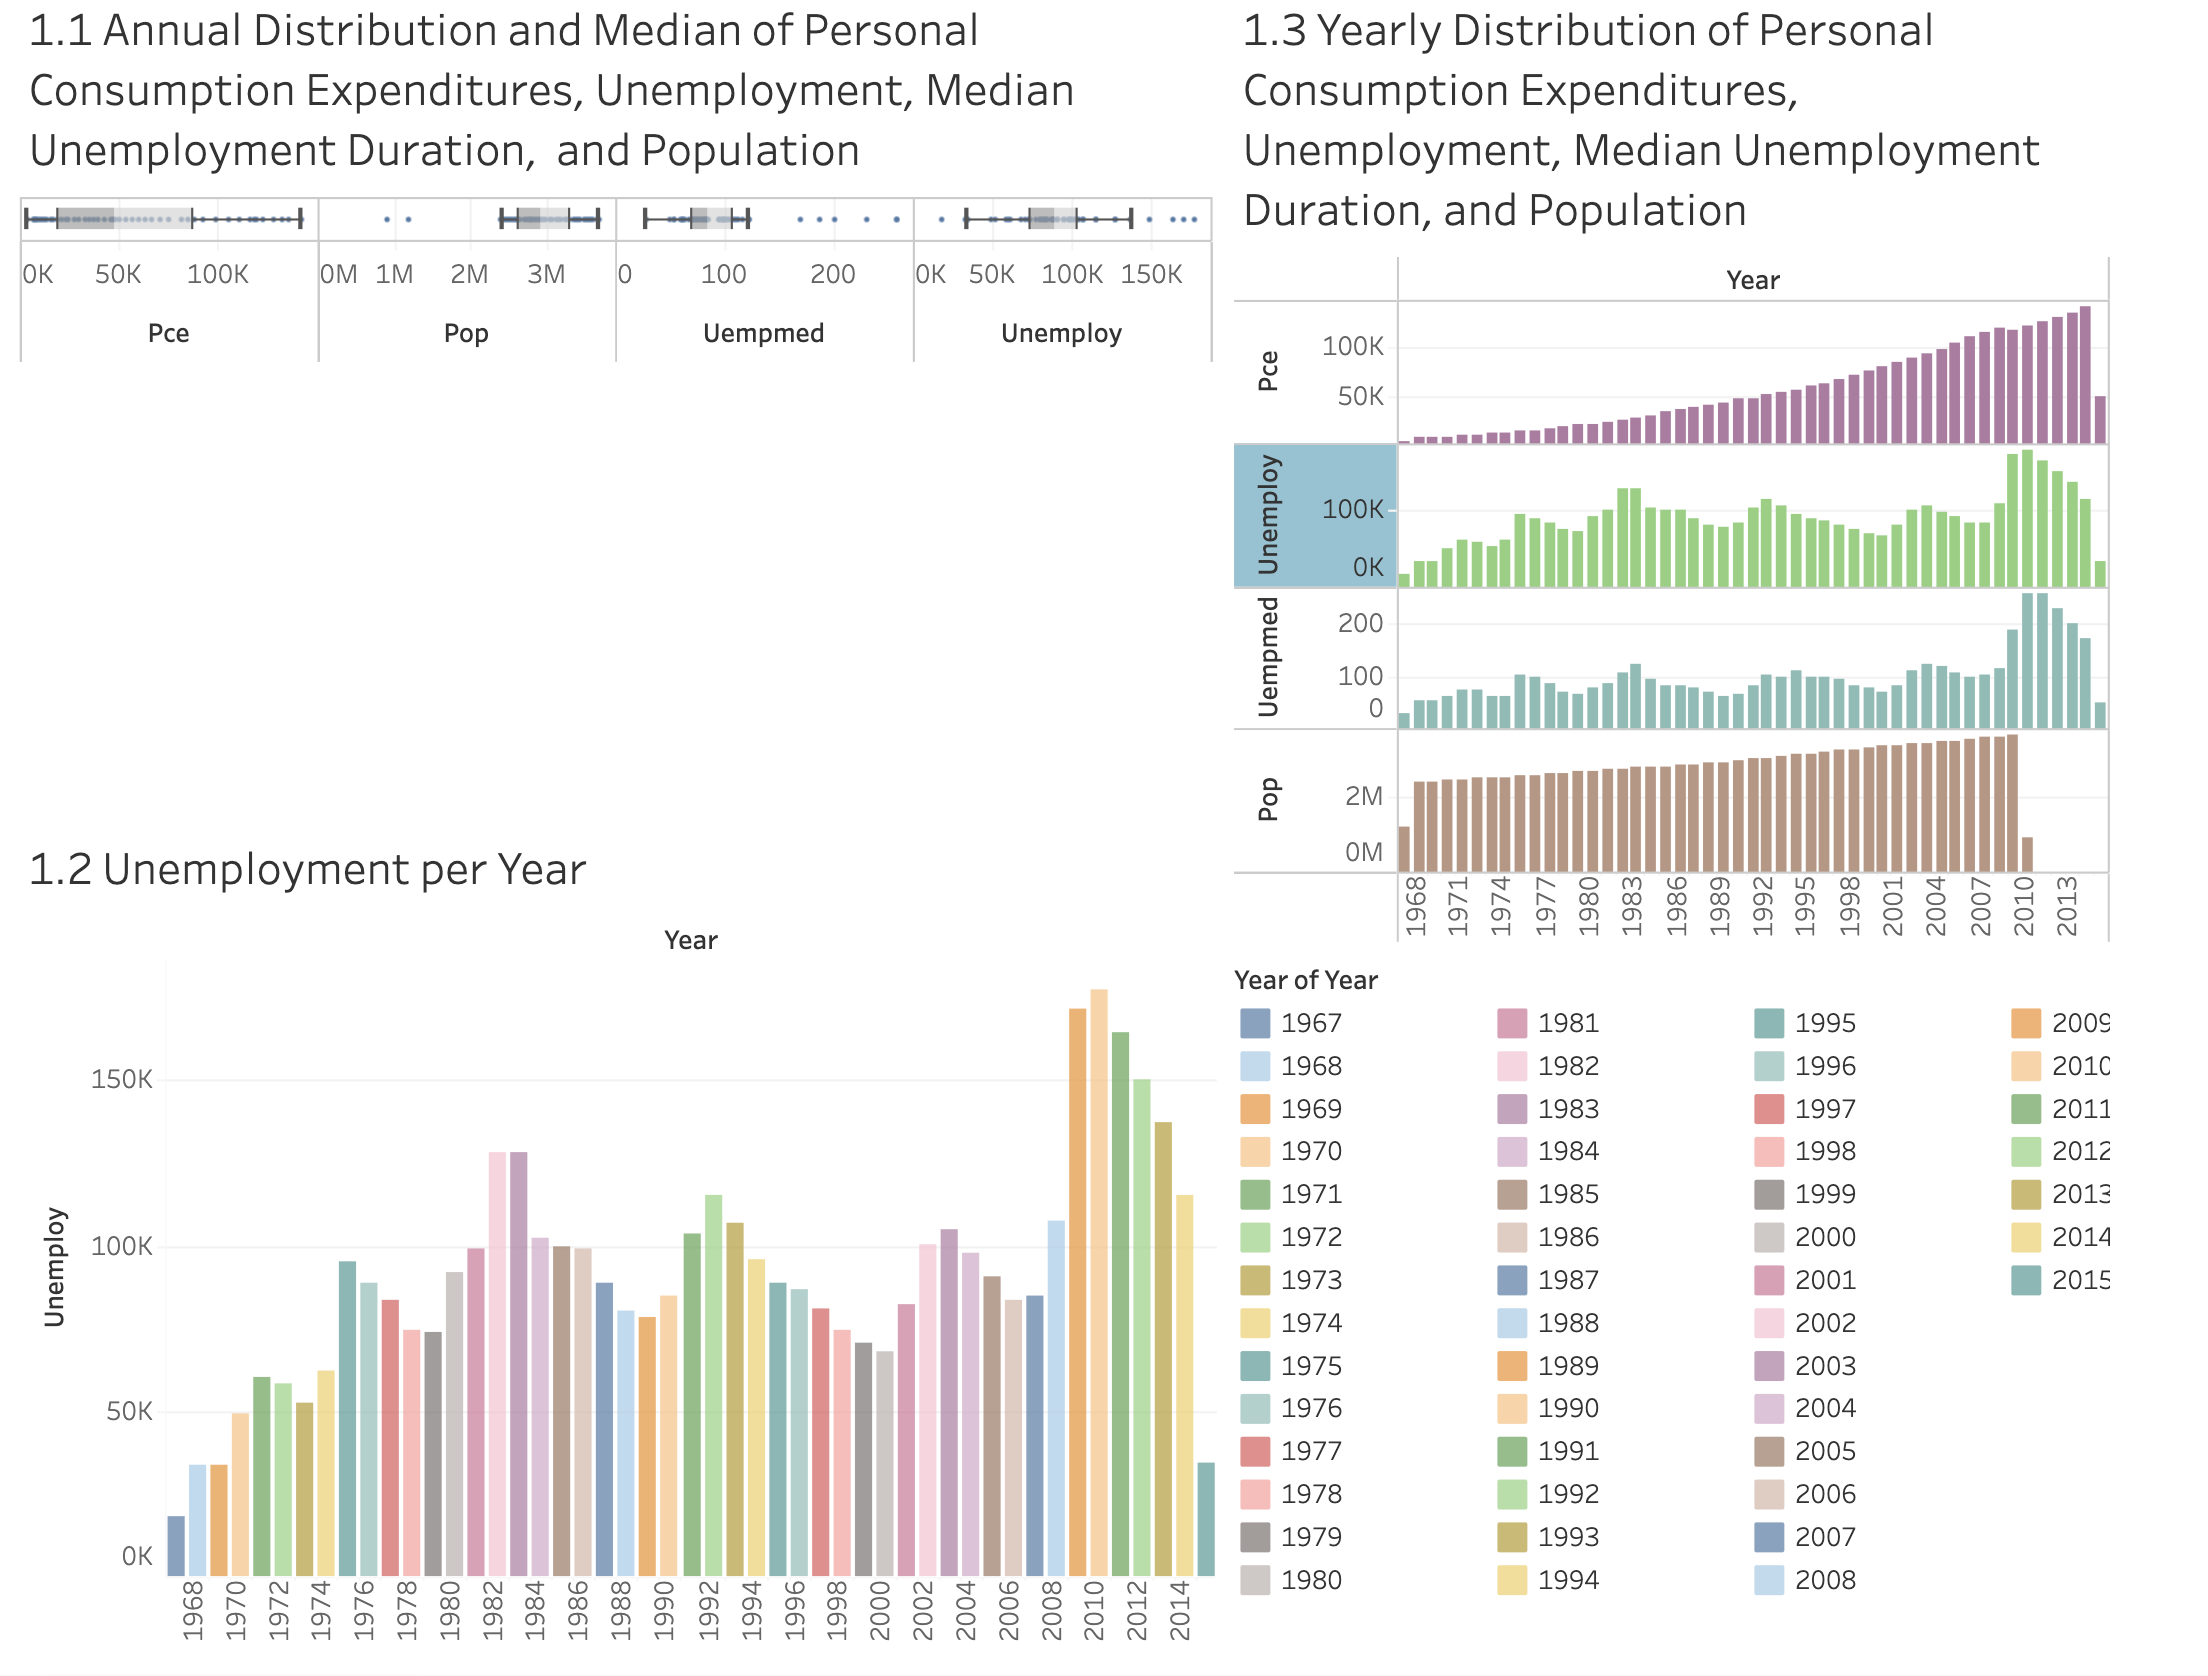
\includegraphics{./dashboard-economics.png}

\textbf{Description}

\textbf{Figure 1.1}

Box plots showing the distribution of the four variables (Pce, Pop,
Uemmped, Unemploy) across multiple years. This gives insight into the
central tendency, spread, and outliers for each variable.

\textbf{Figure 1.2}

A bar chart showing the unemployment count for each year, with different
colors representing different years, emphasizing trends in unemployment
across time.

\textbf{Figure 1.3}

Stacked charts showing how Pce, Unemploy, Uempmed, and Pop have changed
over the years. This provides a timeline for comparing how these
variables behave in relation to one another, revealing patterns of
economic cycles.

\textbf{2nd Dashboard - Individual Project}

Click on this link to see and interact with the dashboard!
\url{https://public.tableau.com/views/IndividualProjectTableau_17262585364150/Dashboard1?:language=en-US&:sid=&:redirect=auth&:display_count=n&:origin=viz_share_link}

\textbf{Variables}

\begin{itemize}
\item
  Crashes

  Total number of traffic crashes reported
\item
  Fatalities

  Number of individuals killed in traffic-related incidents
\item
  Injured persons

  Total number of people injured in traffic accidents
\item
  Vehicles-miles traveled

  Total number of miles driven by all vehicles, measured in millions
\end{itemize}

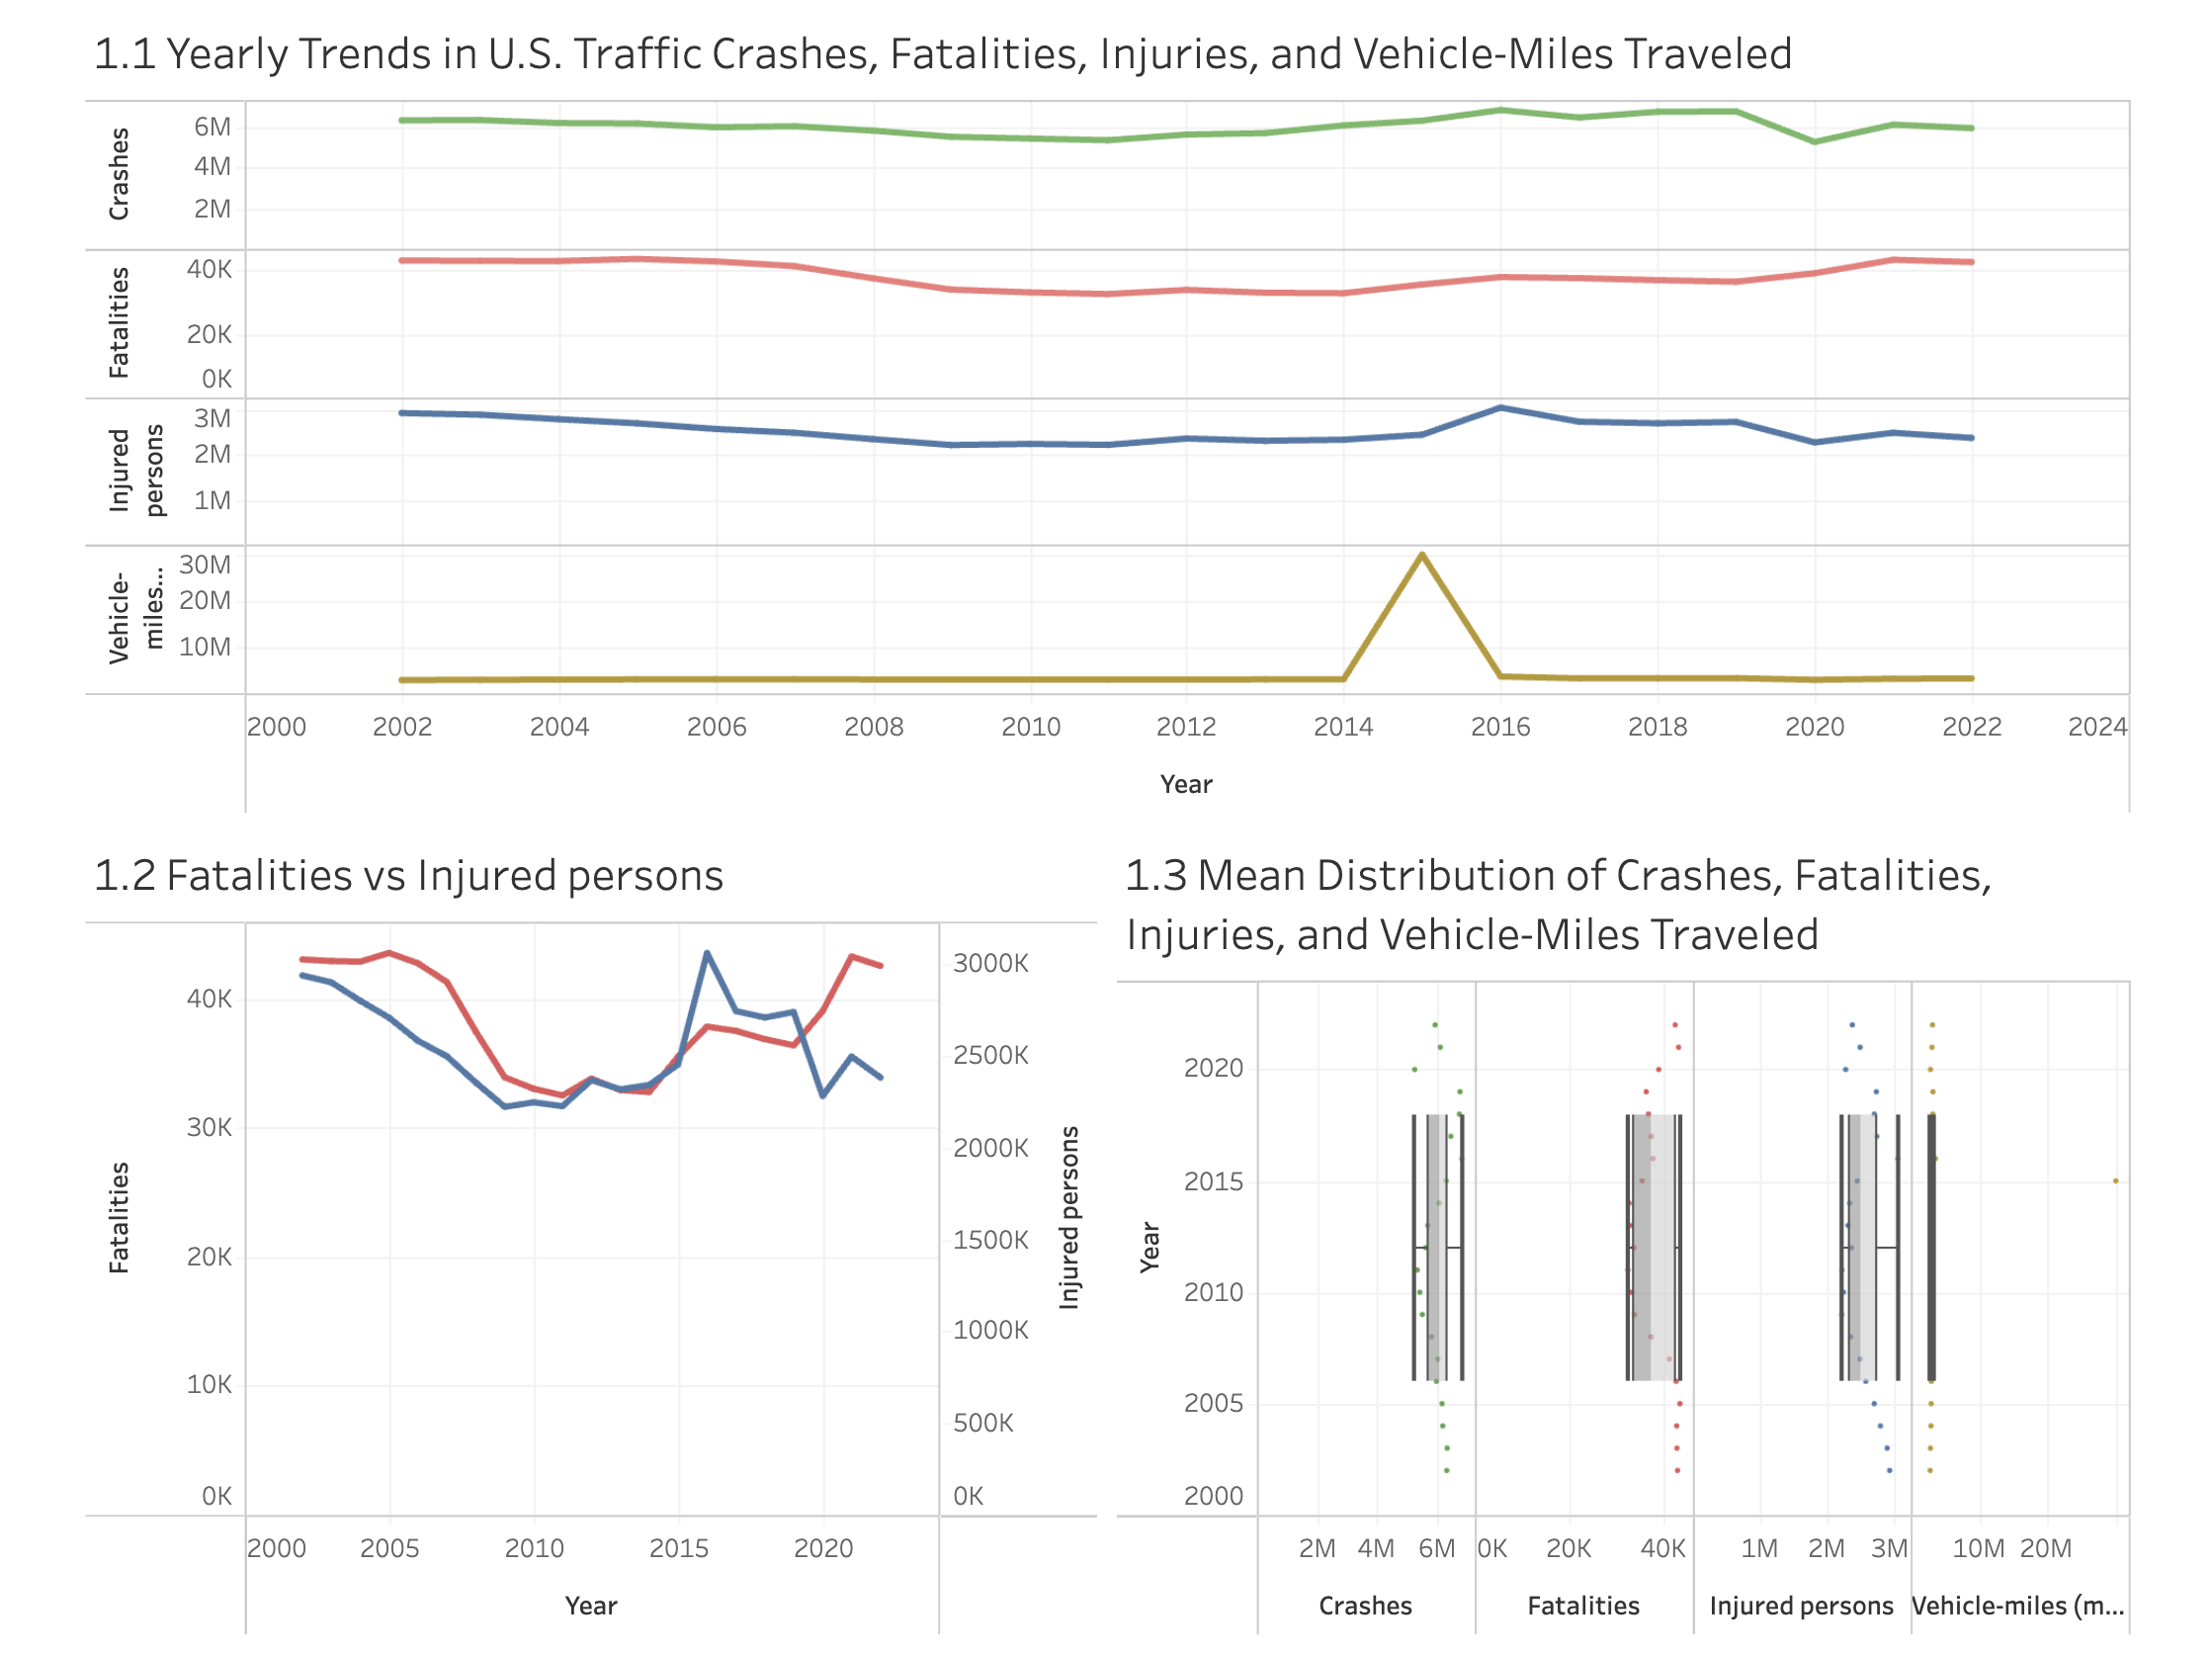
\includegraphics{./dashboard-indivproject.png}

\textbf{Description}

\textbf{Figure 1.1}

This line chart displays the overall trends in key traffic-related
variables over the years. Crashes (green line) have shown a slight
decline but remain relatively stable. Fatalities (red line) have stayed
consistent, fluctuating around 30,000 to 40,000 per year. Injured
persons (blue line) exhibit a gradual downward trend, with a noticeable
dip in 2015, possibly due to reporting changes or other factors.
Vehicle-miles traveled (brown line) show a sharp drop in 2015 but are
generally consistent, indicating steady road usage over the years. The
chart provides a high-level overview of the interactions between these
variables over time.

\textbf{Figure 1.2}

It shows a decreasing trend in injuries until around 2015, after which
it fluctuates. Fatalities also display minor fluctuations but generally
remain around the 30,000 to 40,000 range per year.

\textbf{Figure 1.3}

The boxes represent the interquartile range, while the whiskers capture
the spread of data, offering a clear view of central tendencies (mean)
and variability across the years 2000 to 2023. This chart highlights the
typical values and outliers for crashes, fatalities, injuries, and miles
traveled.

\section{Wednesday}\label{wednesday}

\subsection{Week 1}\label{week-1}

\subsection{Week 2}\label{week-2}

\textbf{Histogram}

In week 2, data sets that I am using is air quality data set. After
cleaning the data set explained below, select all the data and insert
the histogram chart to create the visualization of the data. The
variables for the histogram chart is only the ozone. From the histogram,
it shows the distribution of the ozone, most of the ozone are 1 to 25
ppm.

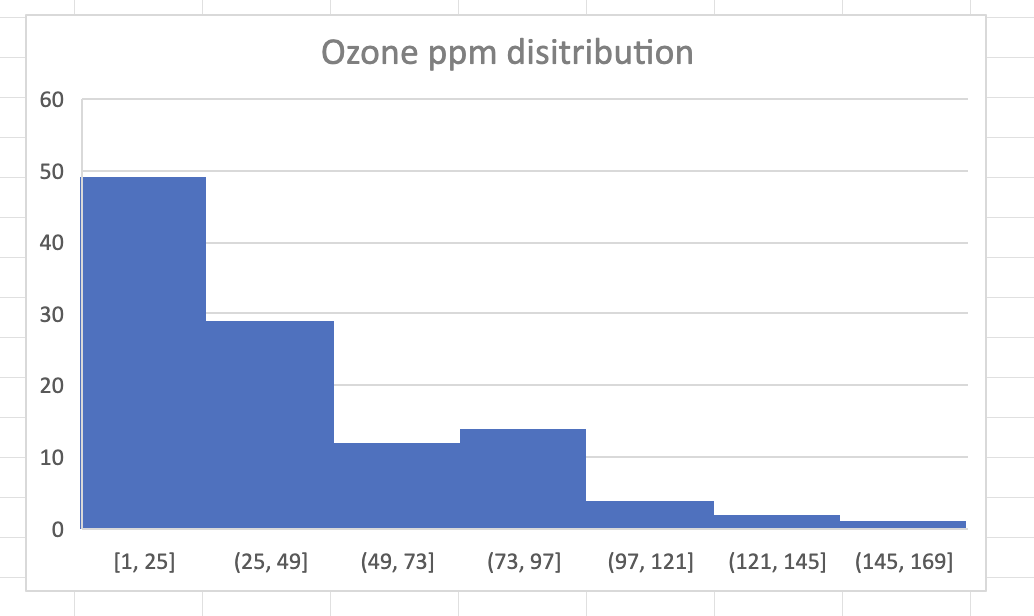
\includegraphics{./histogramozone.png}

\textbf{clean data}

First, from the data, we are going to clean the data, by removing those
that are have the value NA or not available.

1. Select all the data, and search for the filter.

2. Then, it will appear the drop down menu for each column, select the
drop down menu on the first column which is Ozone

3. Select NA. To remove it, select all from the row that has NA until
the bottom and select delete rows 6-151.

4. Select the drop down menu on column Ozone, select all and apply, it
will give back the table, however there's no NA anymore on the Ozone.

Looking at the data, there still some NA on the column B for Solar.R.
Repeat the way just like before. Next, to make it earlier to read the
data, sort the day and month to be in order. Select the column for
month, click the sort from smallest to largest, do the same for day.

\textbf{Scatter plot}

Using the air quality data sets, click on column A(ozone) and D
(temperature) to show the correlation between both of them. After
clicking on both column, I'm going to insert the scatter plot. The
scatter plot shows a relationship between Ozone levels (y-axis) and
Temperature (x-axis). The general trend indicates a positive
correlation: as the temperature increases, the ozone level tends to
increase as well.

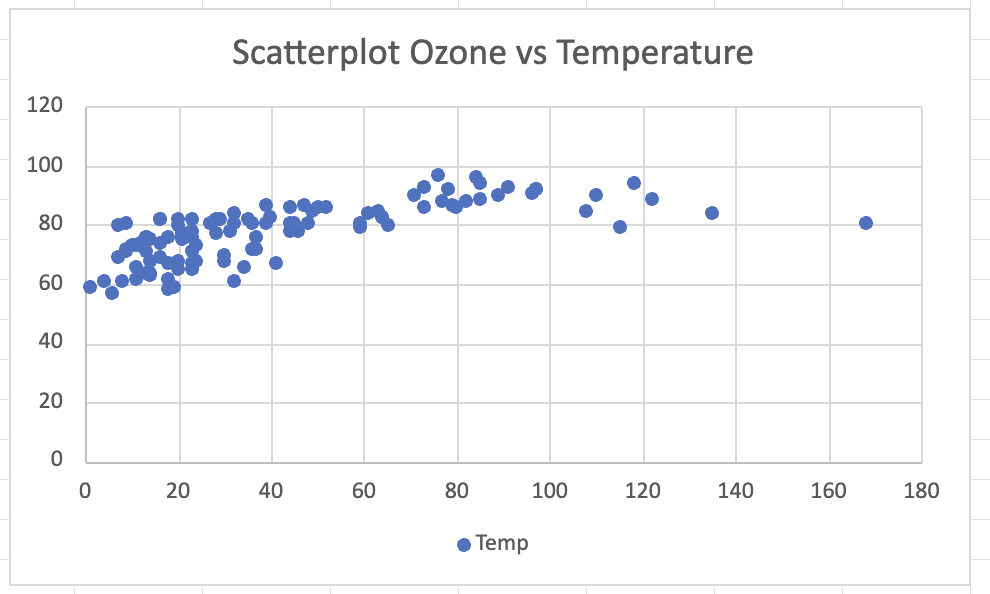
\includegraphics{./scatterplotozone.png}

\textbf{Pivot Table \& Chart}

To make a pivot table and chart, first select all the data, and click
insert. On the let corner, it will appear the pivot menu, press that and
select the create own pivot table. I select and drag ozone, temperature,
Solar. R, and Wind to the value, for the row I'll put only the month.
Then, I change the value field settings to average, this is to provide
the average of ozone, temperature, Solar. R, and Wind monthly. After
doing the pivot table, select that pivot table and insert the pivot
chart to create the visualization.

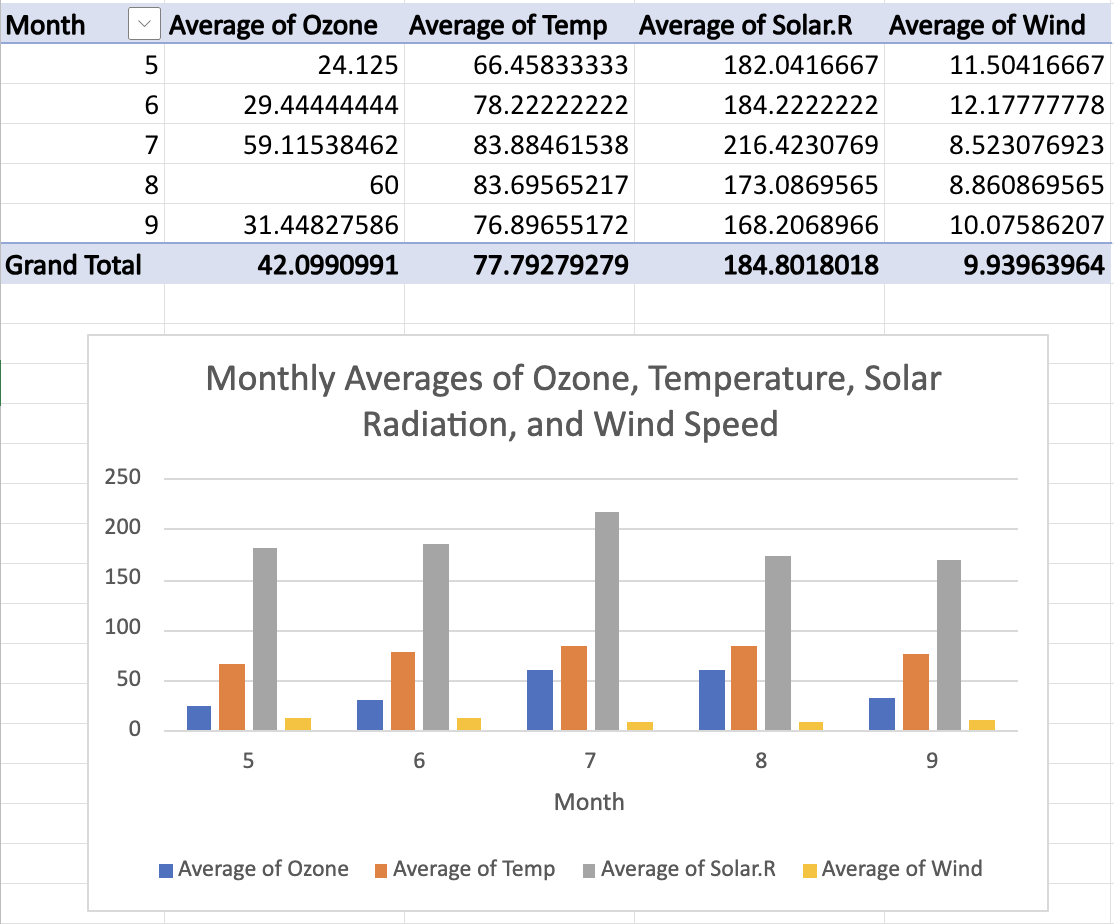
\includegraphics{./pivot1.png}

From the pivot table and chart above, it shows that ozone levels appear
to increase with higher temperature and solar radiation but decrease
with higher wind speeds.

Next, I'm going to provide another pivot table, that shows the average
of ozone, temperature, Solar. R, and Wind daily from day 1 to 31. To do
that, select again the first table, the one that was cleaned, then again
select the pivot table and choose the create own pivot table.

I select and drag ozone, temperature, Solar. R, and Wind to the value,
for the row I'll put only the day. Then, I change the value field
settings to average, this is to provide the average of ozone,
temperature, Solar. R, and Wind per day.

Now, I'm going to add the pivot chart from that new pivot table. I
choose two charts, from those two I can create conclusion and better
visualizations.

From the chart presented below, the average daily of Temperature and
Wind each have a positive correlation, however not with the average
daily of Solar. R and the Ozone. Also, on day 15 it shows the lowest
average of ozone and solar. r.

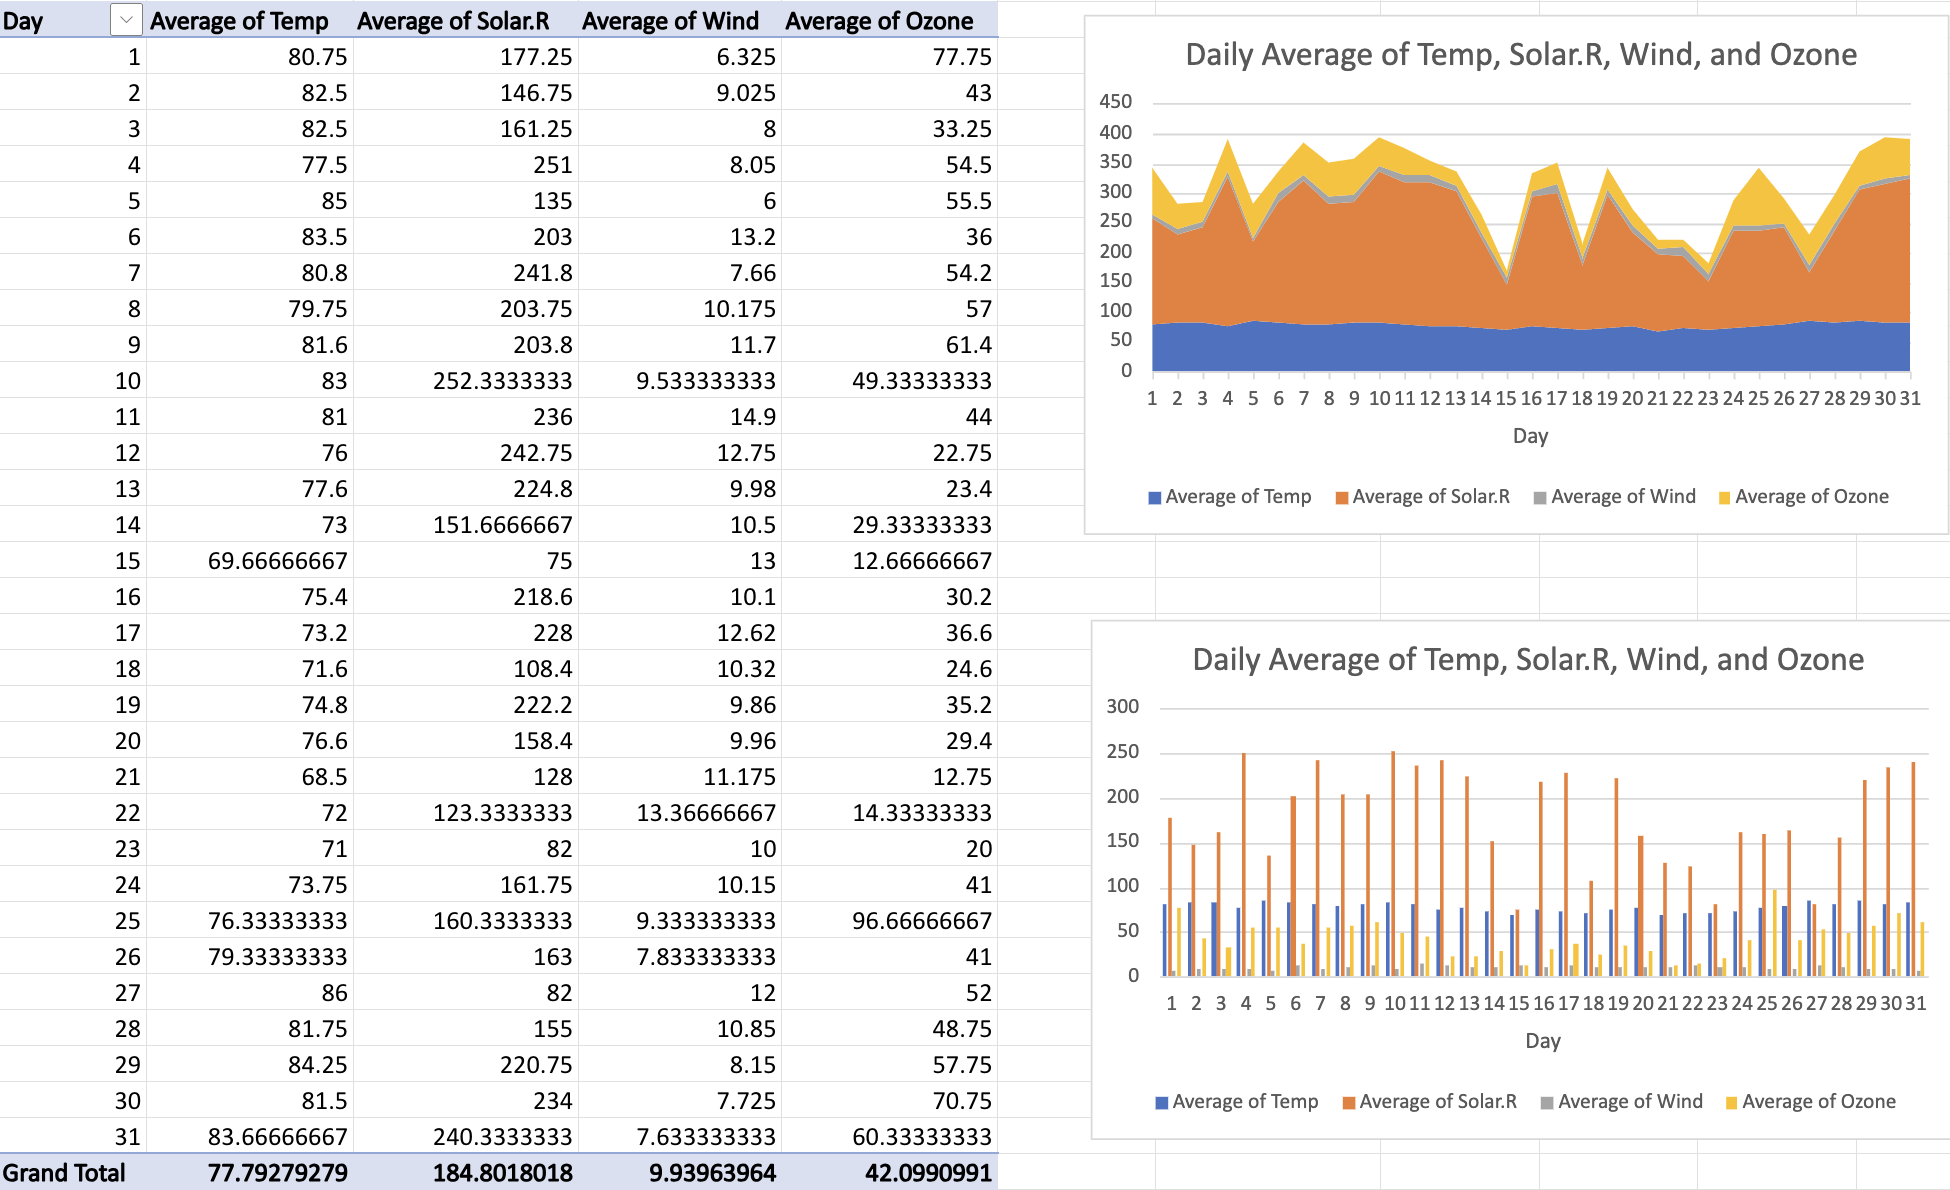
\includegraphics{./pivot2.png}

Third, I'm going to make another pivot table that can show more detailed
on each month per day.I'm going to choose to present the 5th month, so
I'm going to press the drop down menu from the column ``month'' and
select only the 5. Next, the table will only provide the information
from month 5, day 1-31 and the sum of ozone, wind, temp, and solar.r.

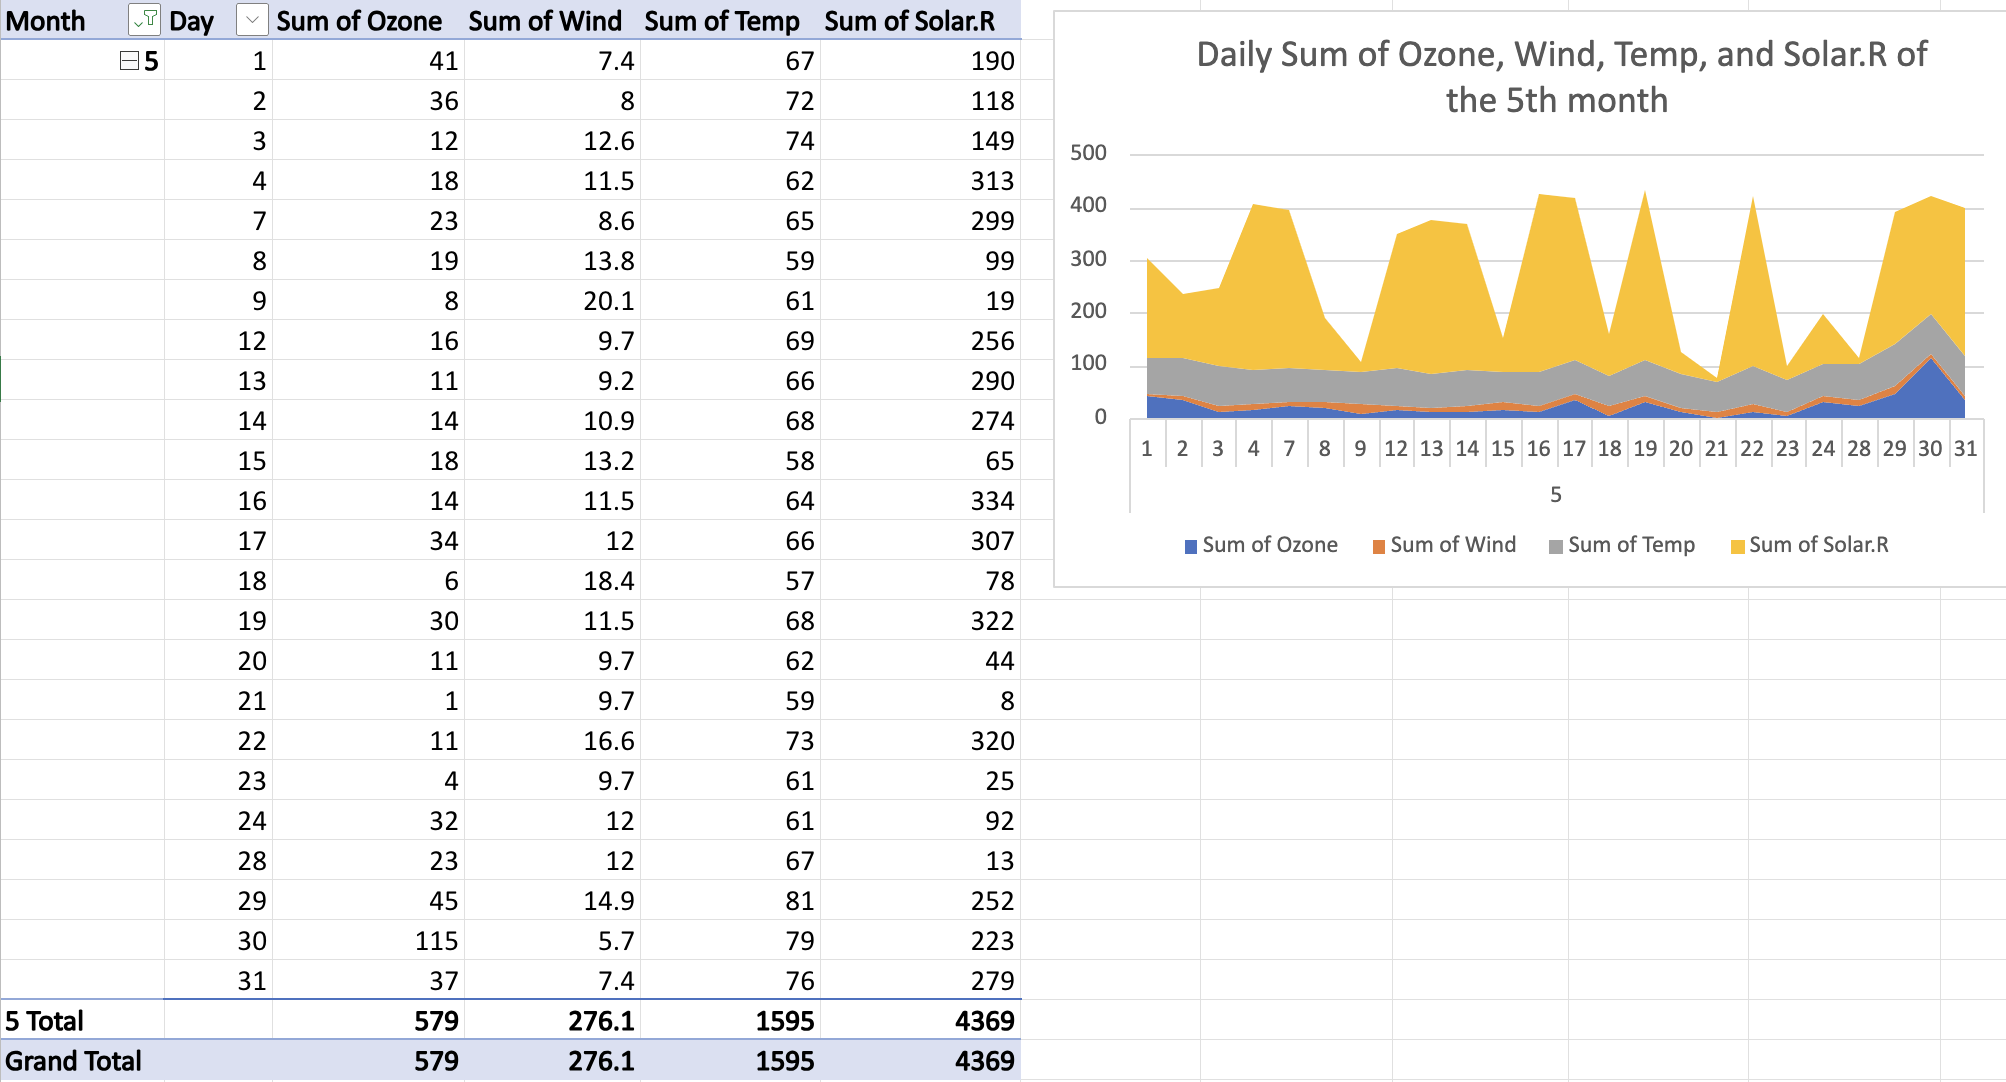
\includegraphics{./pivot3.png}

From the chart, we can see that, on day 30 from the 5th month, it shows
the highest sum of ozone.

\section{Friday - Midterm Projects}\label{friday---midterm-projects}

\subsection{Week 1}\label{week-1-1}

\subsection{Week 2}\label{week-2-1}

\textbf{Who collected the data}

The source that I chose is National Transportation Library (NTL) Data.
There are lots of data sets from NTL, which can be access through
\url{https://ntl.bts.gov/ntl}. Data set that I chose is motor vehicle
safety. This data set is collected by U.S. Department of Transportation,
National Highway Traffic Safety Administration, National Center for
Statistics and Analysis, and Fatality Analysis Reporting System (FARS)
Database. I'm interested in this one, because it is critical to
understand trends in road safety, which is a major public concern. The
data that I collect is from this link
\url{https://www.bts.gov/content/motor-vehicle-safety-data}.

\textbf{Purpose}

Monitoring the trends in motor vehicle safety in the U.S., including
fatalities, injuries, and crashes. It serves to assess the effectiveness
of safety regulations, technology advancements, and policy interventions
over time. From the visualizations, it can improve the safety measures
and highlight the effectiveness of road safety interventions over the
years, making it highly valuable for assessing long-term changes in
traffic-related fatalities and injuries.

\textbf{Variables}

\begin{itemize}
\item
  Fatalities - total number of deaths from motor vehicle crashes
\item
  Injured persons - total number of people injured in motor vehicle
  accidents
\item
  Crashes - total number of motor vehicle crashes
\item
  Vehicles miles traveled - total number of miles driven by vehicles
\end{itemize}

\subsection{Week 5}\label{week-5}

\textbf{Mid Term Project}

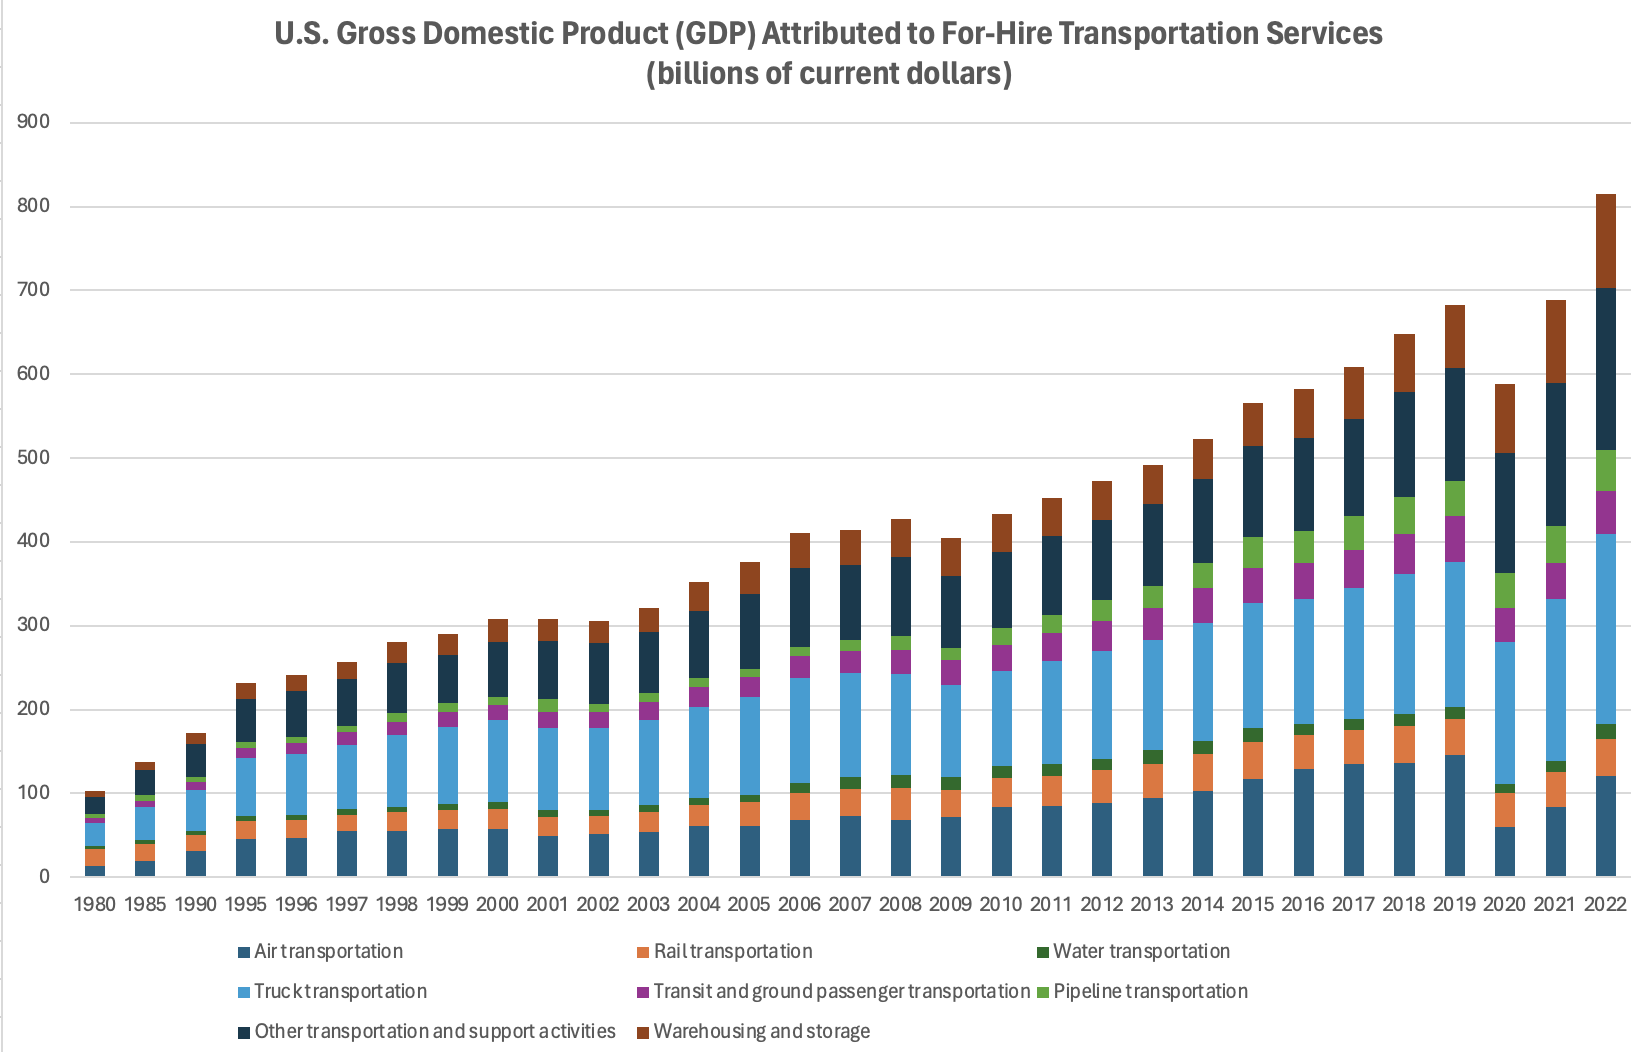
\includegraphics{./GDP-TransportationServices.png}

\textbf{Variables in the Graph:}

\begin{itemize}
\item
  Time (X-axis)

  Years from 1980 to 2022
\item
  GDP (Y-axis)

  U.S. Gross Domestic Product (GDP) attributed to for-hire
  transportation services, measured in billions of current dollars.
\end{itemize}

\textbf{Categories of Transportation Services (Stacked Bars)}

\begin{itemize}
\tightlist
\item
  Air transportation
\item
  Truck transportation
\item
  Rail transportation
\item
  Water transportation
\item
  Pipeline transportation
\item
  Transit and ground passenger transportation
\item
  Other transportation and support activities
\item
  Warehousing and storage
\end{itemize}

\textbf{Key Insights}

The graph illustrates the \textbf{consistent growth of the U.S. GDP from
for-hire transportation services between 1980 and 2022}. Truck and air
transportation sectors contribute the largest shares, with noticeable
growth across all categories post-2010. The overall upward trend
reflects the increasing economic importance of transportation services
in the U.S.

\subsection{Week 8}\label{week-8}

\textbf{Project Presentation}

\textbf{Brief explanation}

\begin{longtable}[]{@{}
  >{\raggedright\arraybackslash}p{(\columnwidth - 0\tabcolsep) * \real{1.0000}}@{}}
\toprule\noalign{}
\endhead
\bottomrule\noalign{}
\endlastfoot
The data set that we chose as a group is the \textbf{U.S. GDP attributed
to for-hire transportation services between 1980 and 2022}. \\
\end{longtable}

\textbf{Variables}

\begin{itemize}
\item
  \ul{Year}

  The year for which the GDP data is recorded from 1980 to 2022.
\item
  \ul{Air transportation}

  GDP attributed to for-hire \textbf{air transportation services}
  (billions of current dollars).
\item
  \ul{Rail transportation}

  GDP attributed to for-hire \textbf{rail transportation services}
  (billions of current dollars).
\item
  \ul{Water transportation}

  GDP attributed to for-hire \textbf{water transportation services}
  (billions of current dollars).
\item
  \ul{Truck transportation}

  GDP attributed to for-hire \textbf{truck transportation services}
  (billions of current dollars).
\item
  \ul{Transit and ground passenger transportation}

  GDP attributed to for-hire \textbf{transit and ground passenger
  transportation services}, such as buses, taxis, etc. (billions of
  current dollars).
\item
  \ul{Pipeline transportation}

  GDP attributed to \textbf{pipeline transportation services}, which
  typically include transportation of natural gas and oil (billions of
  current dollars).
\item
  \ul{Other transportation and support activities}

  GDP attributed to \textbf{other transportation-related services},
  including logistics support activities, courier services, etc.
  (billions of current dollars).
\item
  \ul{Warehousing and storage}

  GDP attributed to \textbf{warehousing and storage services}, which
  include storage of goods and inventory management (billions of current
  dollars).\\
\end{itemize}

\textbf{Purpose}

Analyzing this data as a group can help:

\begin{itemize}
\item
  improve the findings based on overall
\item
  to input necessary changes
\item
  make a solid and strong conclusion based on the findings from
  different perspectives of each of the member
\end{itemize}

\section{Jupyter Notebooks}\label{jupyter-notebooks}

\subsection{Week 4}\label{week-4}

\textbf{This is a markdown title}

in markdown we can create lists:

\begin{itemize}
\tightlist
\item
  item 1
\item
  item 2
\item
  item 3
\end{itemize}

also we can create enumerated list

\begin{enumerate}
\def\labelenumi{\arabic{enumi}.}
\tightlist
\item
  Hola
\item
  Hi
\item
  Namaste
\end{enumerate}

we can do \textbf{bold}, also \emph{italic}

\begin{Shaded}
\begin{Highlighting}[]
\CommentTok{\# List are native to Python}
\ImportTok{import}\NormalTok{ numpy }\ImportTok{as}\NormalTok{ np}
\BuiltInTok{print}\NormalTok{(np.absolute(}\OperatorTok{{-}}\DecValTok{1}\NormalTok{))}
\NormalTok{arr }\OperatorTok{=}\NormalTok{ np.array([}\DecValTok{1}\NormalTok{, }\DecValTok{2}\NormalTok{, }\DecValTok{3}\NormalTok{, }\DecValTok{4}\NormalTok{, }\DecValTok{5}\NormalTok{])}
\BuiltInTok{print}\NormalTok{(arr)}
\end{Highlighting}
\end{Shaded}

\begin{verbatim}
1
[1 2 3 4 5]
\end{verbatim}

\begin{Shaded}
\begin{Highlighting}[]
\CommentTok{\# List are native to Python}
\NormalTok{my\_list }\OperatorTok{=}\NormalTok{ [}\DecValTok{1}\NormalTok{, }\DecValTok{2}\NormalTok{, }\DecValTok{3}\NormalTok{, }\DecValTok{4}\NormalTok{, }\DecValTok{5}\NormalTok{]}
\BuiltInTok{print}\NormalTok{ (my\_list)}
\end{Highlighting}
\end{Shaded}

\begin{verbatim}
[1, 2, 3, 4, 5]
\end{verbatim}

\begin{Shaded}
\begin{Highlighting}[]
\CommentTok{\# We will be using a lot of data frames, so we need pandas library}
\CommentTok{\# Panda allows us to make small spreadsheets, there will be rows and columns}
\ImportTok{import}\NormalTok{ pandas }\ImportTok{as}\NormalTok{ pd}
\NormalTok{data }\OperatorTok{=}\NormalTok{ \{}\StringTok{\textquotesingle{}Ozone\textquotesingle{}}\NormalTok{: [}\DecValTok{41}\NormalTok{, }\DecValTok{36}\NormalTok{, }\DecValTok{12}\NormalTok{], }\StringTok{\textquotesingle{}Temp\textquotesingle{}}\NormalTok{: [}\DecValTok{67}\NormalTok{, }\DecValTok{72}\NormalTok{, }\DecValTok{74}\NormalTok{]\}}
\NormalTok{df }\OperatorTok{=}\NormalTok{ pd.DataFrame(data)}
\BuiltInTok{print}\NormalTok{(df)}
\end{Highlighting}
\end{Shaded}

\begin{verbatim}
   Ozone  Temp
0     41    67
1     36    72
2     12    74
\end{verbatim}

\textbf{4. Loading CSV files} To load files into a \texttt{DataFrame} ,
we use the pandas function \texttt{read\_csv};

\begin{Shaded}
\begin{Highlighting}[]
\CommentTok{\# Load and analyze data from a CSV file named airquality\_datasets.csv using the pandas library}
\NormalTok{df }\OperatorTok{=}\NormalTok{ pd.read\_csv(}\StringTok{\textquotesingle{}airquality\_datasets.csv\textquotesingle{}}\NormalTok{)}
\end{Highlighting}
\end{Shaded}

\begin{Shaded}
\begin{Highlighting}[]
\CommentTok{\# df.info () {-}\textgreater{} displays the structure and non{-}null counts of the DataFrame.}
\CommentTok{\# df.describe () {-}\textgreater{} provides summary statistics such as mean, standard deviation, minimum, and maximum values for each column.}
\BuiltInTok{print}\NormalTok{(df.info())}
\BuiltInTok{print}\NormalTok{(df.describe())}
\end{Highlighting}
\end{Shaded}

\begin{verbatim}
<class 'pandas.core.frame.DataFrame'>
RangeIndex: 153 entries, 0 to 152
Data columns (total 6 columns):
 #   Column   Non-Null Count  Dtype  
---  ------   --------------  -----  
 0   Ozone    116 non-null    float64
 1   Solar.R  146 non-null    float64
 2   Wind     153 non-null    float64
 3   Temp     153 non-null    int64  
 4   Month    153 non-null    int64  
 5   Day      153 non-null    int64  
dtypes: float64(3), int64(3)
memory usage: 7.3 KB
None
            Ozone     Solar.R        Wind        Temp       Month         Day
count  116.000000  146.000000  153.000000  153.000000  153.000000  153.000000
mean    42.129310  185.931507    9.957516   77.882353    6.993464   15.803922
std     32.987885   90.058422    3.523001    9.465270    1.416522    8.864520
min      1.000000    7.000000    1.700000   56.000000    5.000000    1.000000
25%     18.000000  115.750000    7.400000   72.000000    6.000000    8.000000
50%     31.500000  205.000000    9.700000   79.000000    7.000000   16.000000
75%     63.250000  258.750000   11.500000   85.000000    8.000000   23.000000
max    168.000000  334.000000   20.700000   97.000000    9.000000   31.000000
\end{verbatim}

\textbf{Instant data view} - JupyterLab allows us to instantly view the
structure and data types of the columns within the DataFrame by using
df.info(). This displays a concise summary of each column, including the
number of non-null entries and the type of data (e.g., float64, int64).
- This feature makes it easy to verify that the data types (like floats
for Temp, Ozone, Wind, etc.) align with the expected values from the CSV
file, ensuring the data is in the correct format for further analysis
and visualization.

\begin{Shaded}
\begin{Highlighting}[]
\ImportTok{import}\NormalTok{ matplotlib.pyplot }\ImportTok{as}\NormalTok{ plt}

\CommentTok{\# Ozone Histogram}
\NormalTok{plt.figure(figsize}\OperatorTok{=}\NormalTok{(}\DecValTok{8}\NormalTok{, }\DecValTok{6}\NormalTok{))}
\NormalTok{plt.hist(df[}\StringTok{\textquotesingle{}Ozone\textquotesingle{}}\NormalTok{].dropna(), bins}\OperatorTok{=}\DecValTok{20}\NormalTok{, color}\OperatorTok{=}\StringTok{\textquotesingle{}blue\textquotesingle{}}\NormalTok{, edgecolor}\OperatorTok{=}\StringTok{\textquotesingle{}black\textquotesingle{}}\NormalTok{)}
\NormalTok{plt.title(}\StringTok{\textquotesingle{}Distribution of Ozone Levels\textquotesingle{}}\NormalTok{)}
\NormalTok{plt.xlabel(}\StringTok{\textquotesingle{}Ozone (ppb)\textquotesingle{}}\NormalTok{)}
\NormalTok{plt.ylabel(}\StringTok{\textquotesingle{}Frequency\textquotesingle{}}\NormalTok{)}
\NormalTok{plt.show()}

\CommentTok{\# Temp Histogram}
\NormalTok{plt.figure(figsize}\OperatorTok{=}\NormalTok{(}\DecValTok{8}\NormalTok{, }\DecValTok{6}\NormalTok{))}
\NormalTok{plt.hist(df[}\StringTok{\textquotesingle{}Temp\textquotesingle{}}\NormalTok{].dropna(), bins}\OperatorTok{=}\DecValTok{20}\NormalTok{, color}\OperatorTok{=}\StringTok{\textquotesingle{}orange\textquotesingle{}}\NormalTok{, edgecolor}\OperatorTok{=}\StringTok{\textquotesingle{}black\textquotesingle{}}\NormalTok{)}
\NormalTok{plt.title(}\StringTok{\textquotesingle{}Distribution of Temperature\textquotesingle{}}\NormalTok{)}
\NormalTok{plt.xlabel(}\StringTok{\textquotesingle{}Temperature (°F)\textquotesingle{}}\NormalTok{)}
\NormalTok{plt.ylabel(}\StringTok{\textquotesingle{}Frequency\textquotesingle{}}\NormalTok{)}
\NormalTok{plt.show()}
\end{Highlighting}
\end{Shaded}

\begin{figure}[H]

{\centering 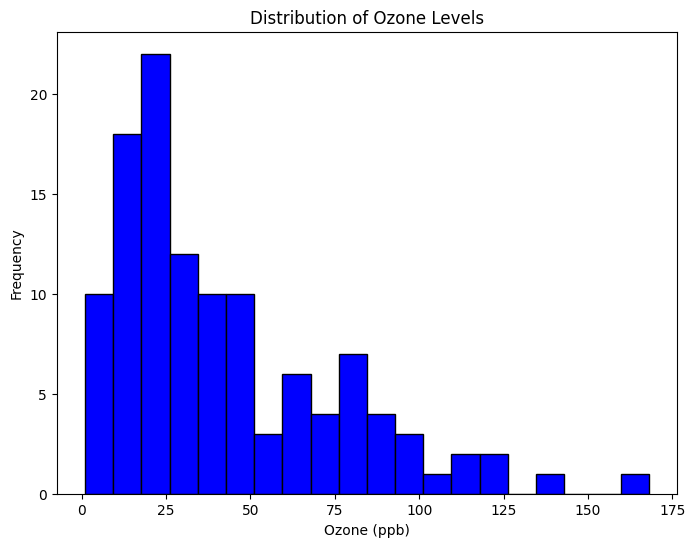
\includegraphics{Tut2_Python_Tako_092024_files/Tut2_Python_Tako_092024_8_0.png}

}

\caption{png}

\end{figure}%%
\begin{figure}[H]

{\centering 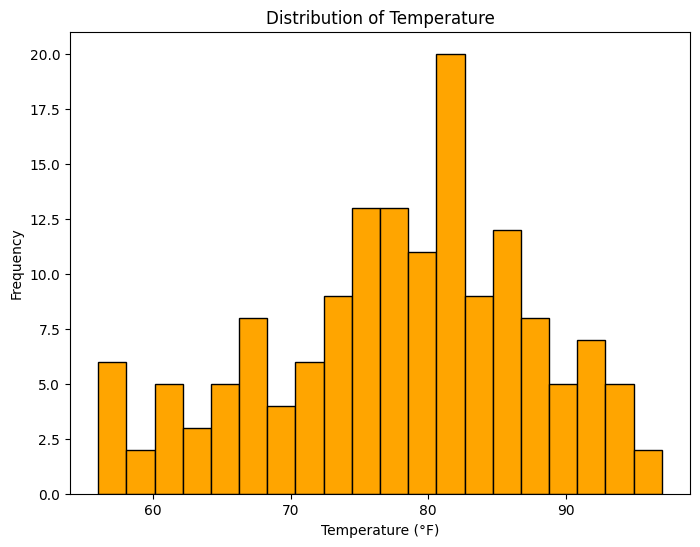
\includegraphics{Tut2_Python_Tako_092024_files/Tut2_Python_Tako_092024_8_1.png}

}

\caption{png}

\end{figure}%

\textbf{Visual Insights} - We can quickly identify trends and the spread
of values. - Peaks in the histograms indicate where data points are
densely clustered, revealing common or typical readings in the dataset.

\chapter{Caleb Pena}\label{caleb-pena}

This page contains all of Caleb Pena's submissions this semester
organized into different sections.

\section{Wednesday}\label{wednesday-1}

\subsection{Week 1}\label{week-1-2}

\subsection{Week 2}\label{week-2-2}

\textbf{Wednesday, September 4, 2024}

I am using the airquality dataset, which is a collection of data
collected from 153 observations based on 6 different variables. These
variables include:

Ozone (Numeric) - Mean ozone in parts per billion from 1300 to 1500
hours at Roosevelt Island

Solar R (Numeric) - Solar radiation in Langleys in the frequency band
4000--7700 Angstroms from 0800 to 1200 hours at Central Park

Wind (Numeric) - Average wind speed in miles per hour at 0700 and 1000
hours at LaGuardia Airport

Temp (Numeric) - Maximum daily temperature in degrees Fahrenheit at La
Guardia Airport

Month (Numeric) - Months from May to September

Day (Numeric) - Days of the months ranging from 1 to 31

I am using Excel to clean the data, which removes all the rows which
have N/A values, and I did an exploration analysis.

\textbf{Ozone vs Temperature Histogram}

This histogram represents the amount of temperature values calculated
within each border of values of ozone. For example, in the range of
ozone level between 1 and 25, there were 49 temperature values recorded.

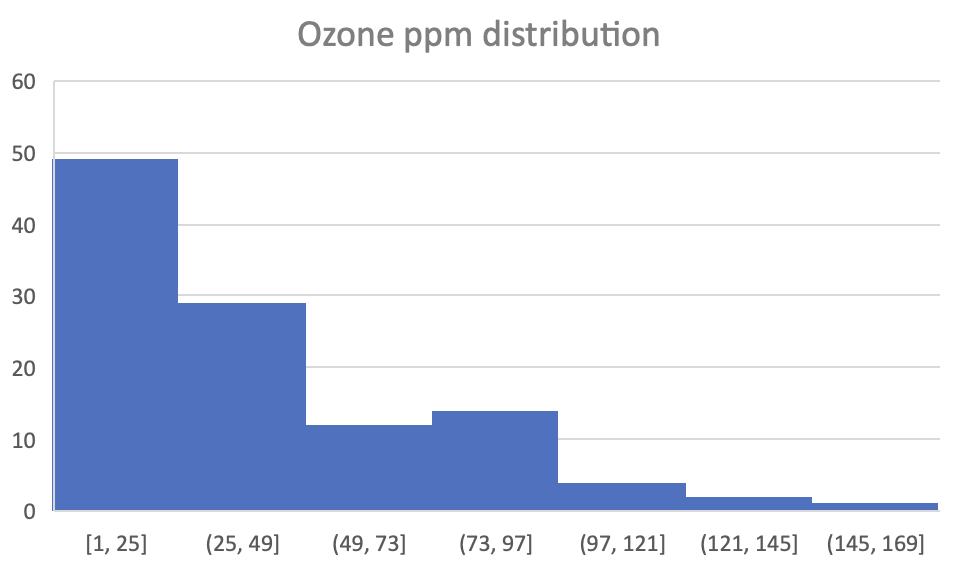
\includegraphics{Hist_Ozone_Pena.png}

\textbf{Ozone vs Temperature Scatter Plot}

This scatter plot displays the correlation between the ozone levels and
the temperature values recorded within these five months. As the ozone
level increased, so did the temperature value, with one outlier.

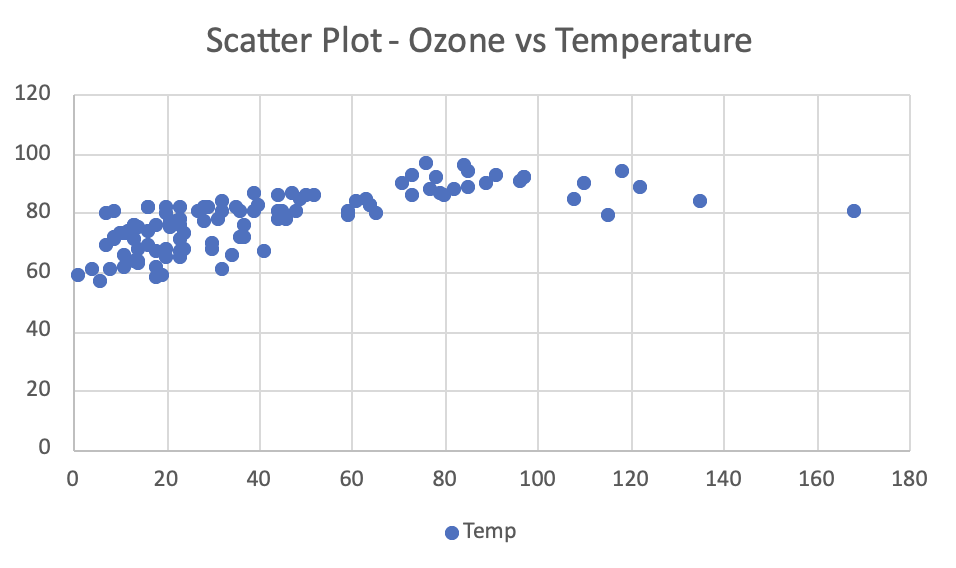
\includegraphics{Scat_Oz_Temp_Pena.png}

\textbf{My First PivotTable}

This PivotTable displays the average values of each variable for each of
the five months.

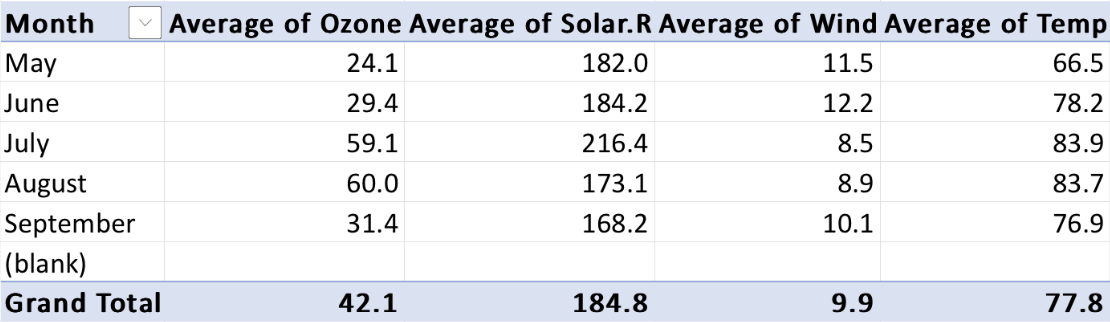
\includegraphics{PivotTable1_Summary_Variables_Pena.png}

\textbf{My Second PivotTable}

This PivotTable displays the average temperature values for each day of
each month.

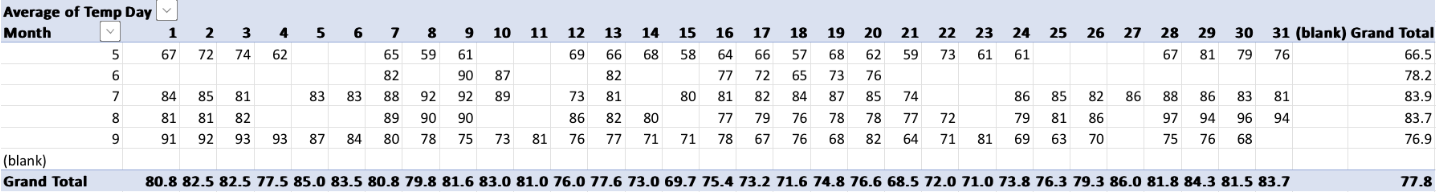
\includegraphics{PivotTable2_Average_Temp_Pena.png}

\subsection{Week 3}\label{week-3}

\textbf{Wednesday, September 11}

The data from the Cars dataset was recorded in the 1920s and focuses on
two different variables:

Speed (Numerical) - The speed in mph at which the car was traveling Stop
Distance (Numerical) - The distance in ft that it took for the car to
stop while traveling a specific speed

This is the dashboard: 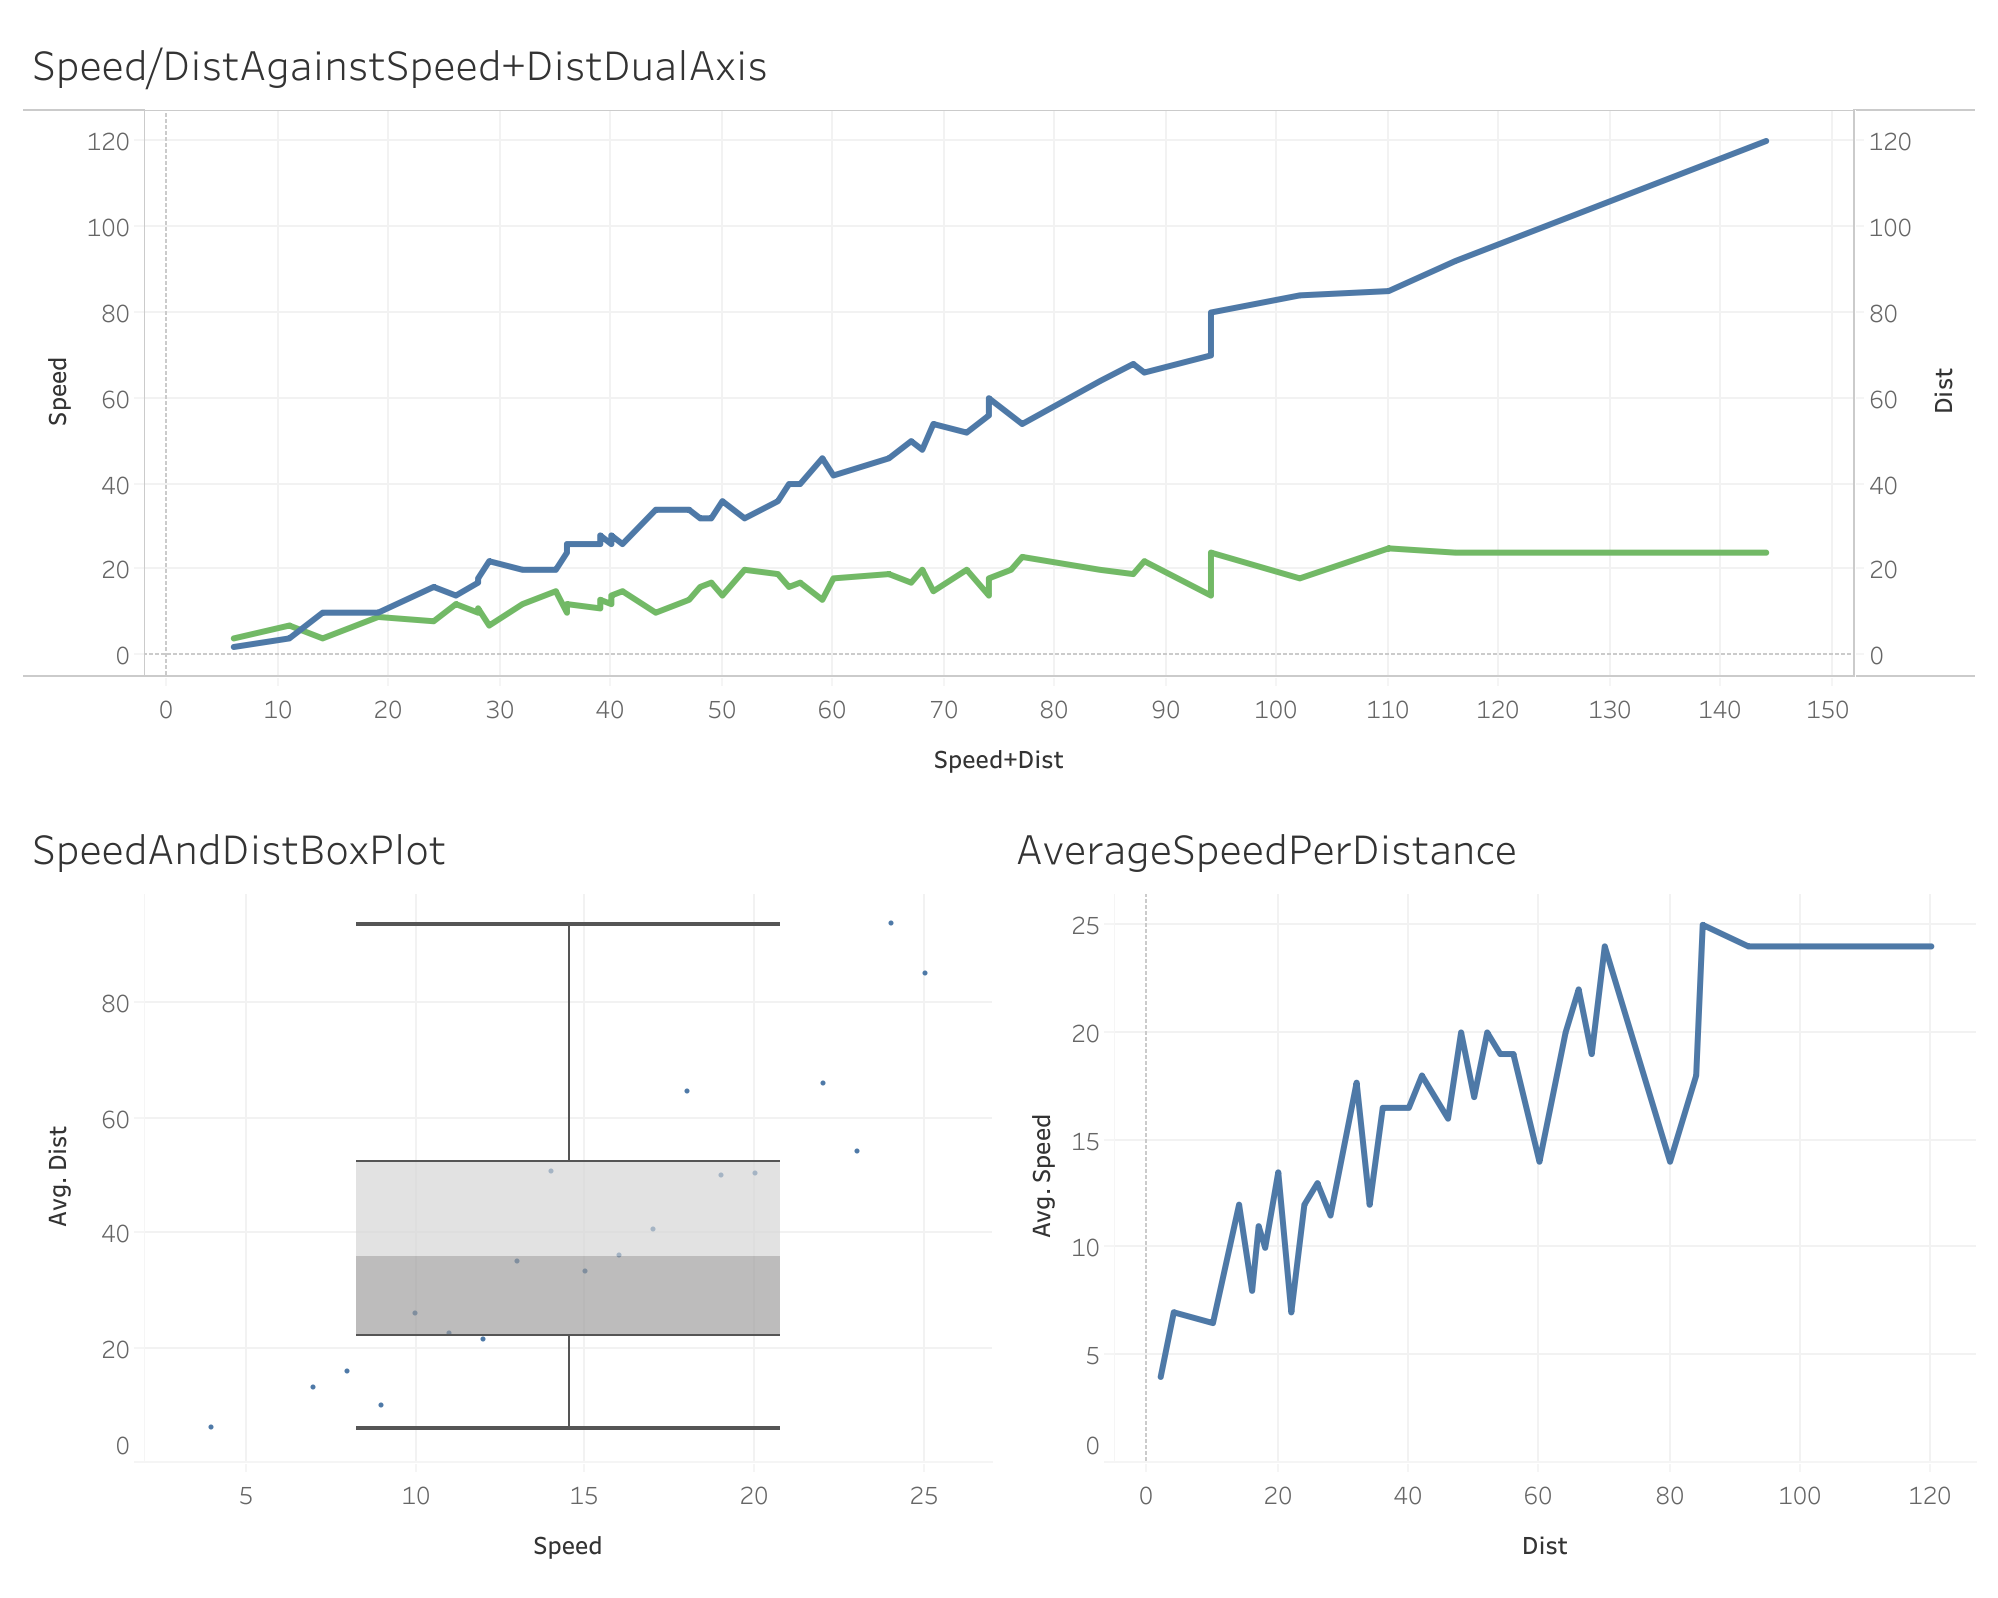
\includegraphics{CarsDatasetDashboard.png}

The graph ``Speed/DistAgainstSpeed+DistDualAxis'' was a dual axis plot
that measured the variables speed and stop distance against a new
calculated variable called speed+dist. This graph simply shows how the
distance values have a much greater numerical value than the speed
values.

The graph ``SpeedAndDistBoxPlot'' was a box plot that measured the
average distance per each speed value and calculated all the data into
one box plot. This plot shows the different values for average stopping
distance in comparison to all the speed values.

The graph ``AverageSpeedPerDistance'' is a line plot that calculates the
average speed per each distance value. There is a correlation between
the values of average speed and distance; as distance values increase,
the average speed of which the car was traveling also increases.

\section{Friday - Midterm Projects}\label{friday---midterm-projects-1}

\subsection{Week 1}\label{week-1-3}

\subsection{Week 2}\label{week-2-3}

\textbf{Friday, September 6, 2024}

Using the same airquality datasets, I worked on creating PivotCharts
from previous and new PivotTables comparing different values and
variables.

\textbf{PivotChart1 - Average Variable Values by `Month'}

This pivot table produced this chart. These are the average values of
each variables for each of the five months. The PivotChart shows the
comparison between each of the variables and how each one increases or
decreases throughout the five months.

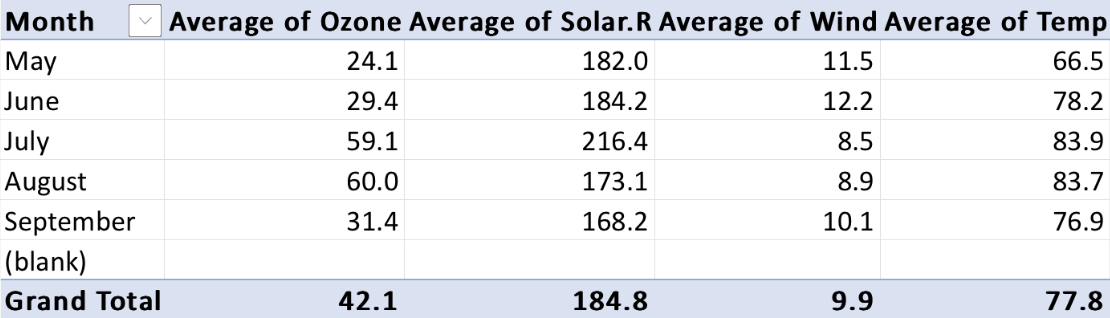
\includegraphics{PivotTable1_AverageVariableValues_Pena.png}

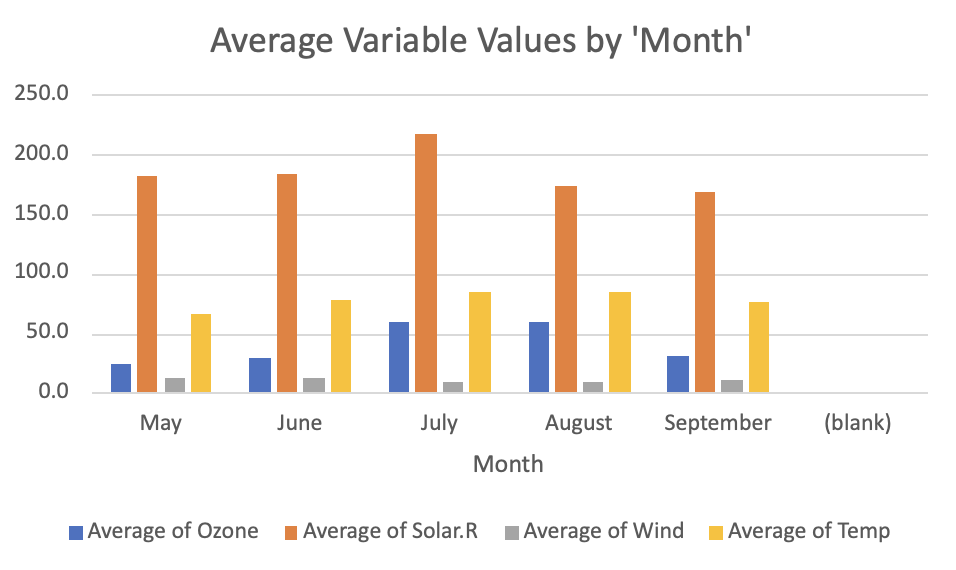
\includegraphics{PivotChart1_AverageVariableValues_Pena.png}

\textbf{PivotChart2 - Average Ozone Values by `Temp'}

This pivot table produced this chart. This PivotChart displays the
average ozone values for each temperature value that was recorded. As
the temperature values increase, the average values for the ozone can be
seen to also increase in a correlated way.

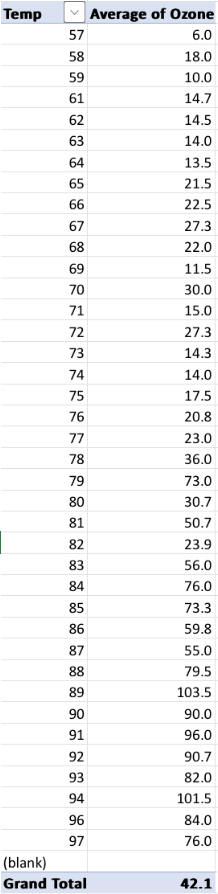
\includegraphics{PivotTable2_AverageOzoneByTemp_Pena.png}

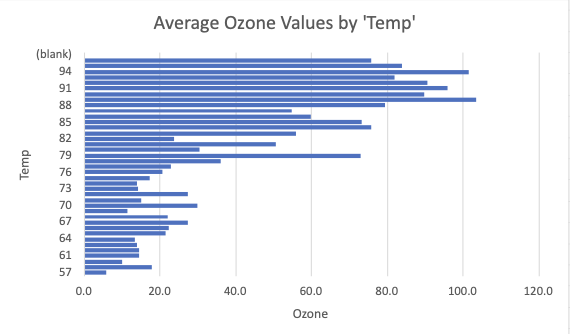
\includegraphics{PivotChart2_AverageOzoneByTemp_Pena.png}

\textbf{PivotChart3 - Average Temp and Ozone Values by `Wind'}

This pivot table produced this chart. This PivotChart displays the
average values of both temperature and ozone for each wind value
recorded. From the chart, it is evident that as the wind values
increase, the average values for temperature seem to slightly decrease
and the average values for the ozone levels seem to greatly decrease.

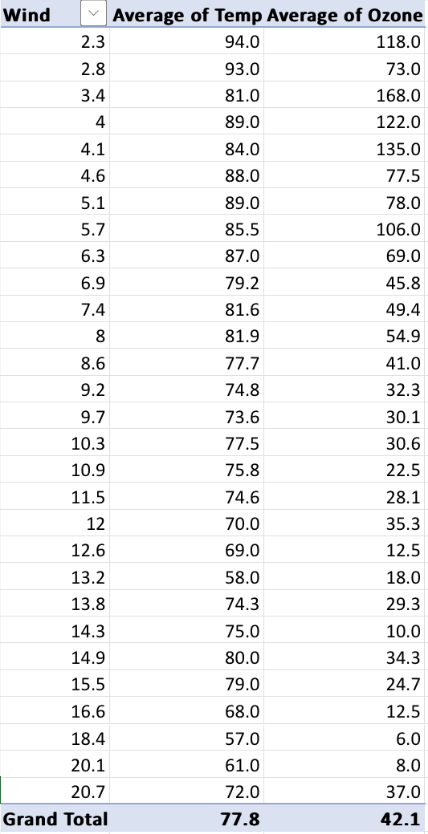
\includegraphics{PivotTable3_AverTempOzoneByWind_Pena.png}

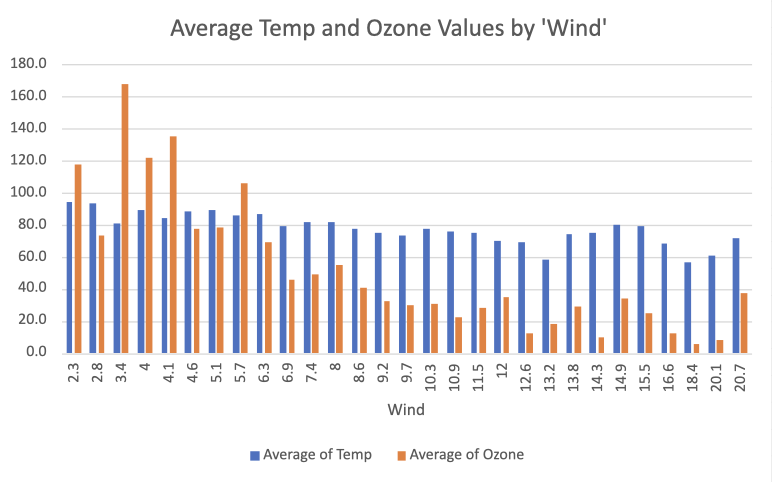
\includegraphics{PivotChart3_AverTempOzoneByWind_Pena.png}

\textbf{Newport Oregon Oceanographic Temperature Dataset}

Starting off in the year 1996, a group of NOAA Fisheries and Oregon
State University Scientists sampled the Newport Hydrographic Line
fortnightly to understand changing ocean conditions. The various
variable data was collected from a station located 5 miles off the coast
of Newport, Oregon. The scientists sampled and collected data regarding
seven different variables:

Day (Numerical) - The specific day of the month in which the data was
sampled.

Month (Numerical) - The specific month of the year in which the data was
sampled.

Year (Numerical) - The specific year in which the data was sampled.

Temperature (Numerical) - Oceanographic, temperature data collected from
a 50 m water depth.

Oxygen (Numerical) - Oceanographic, oxygen data collected from a 50 m
water depth.

Northern Copepod Biomass (Numerical) - Copepod community data collected
from from vertical net samples on the northern area

Southern Copepod Biomass (Numerical) - Copepod community data collected
from from vertical net samples on the southern area

\textbf{Visualizations}

The descriptive statistics of all the water temperatures sampled
throughout the 28 years. The average temperature of all collective 28
years is 8.75 ºC. The lowest temperature recorded of all 28 years is
6.92 ºC and the highest temperature recorded from all 28 years is 14.65
ºC.

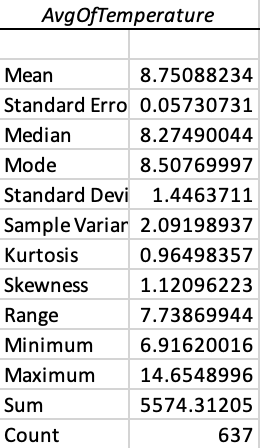
\includegraphics{TemperatureStats.png}

The peak temperatures of the water during the winter have a higher
average than the peak temperatures of the water during the summer.

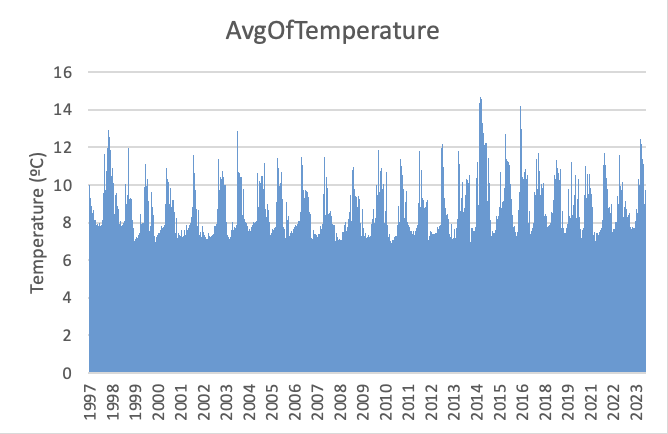
\includegraphics{TemperatureData.png}

Through the dot plot, the average of the temperatures is 8.75 ºC as most
of the dot population is visible there.

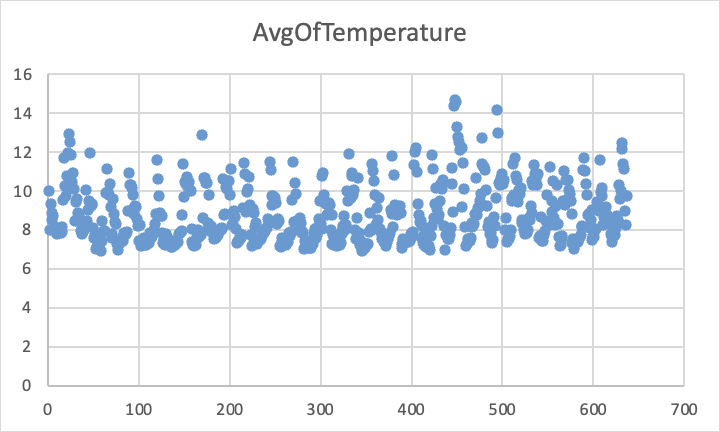
\includegraphics{TemperatureAverage.png}

The average temperatures of all collective 28 years gathered within each
month. During the summer months, the averages are lower. During the
winter months, the averages are higher.

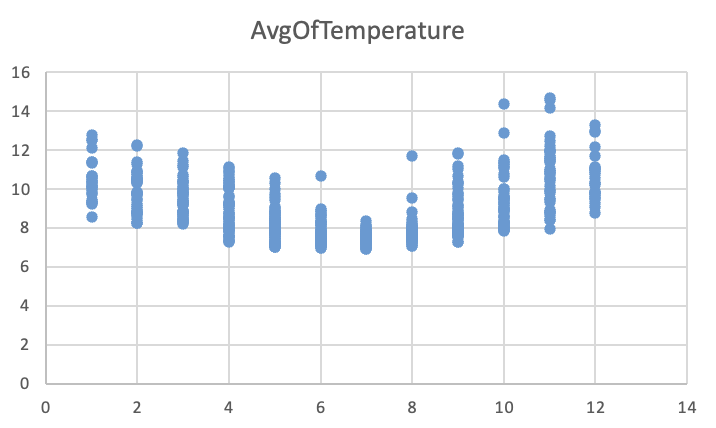
\includegraphics{TemperatureMonthAverage.png} \#\#\# Week 3

\subsection{Week 3}\label{week-3-1}

\textbf{Friday, September 13}

The Oceanographic data from the Newport Line along Oregon was gathered
from 1996 - present and focuses on seven different variables.

Sample Date (Date) - The exact date of which the rest of the variables
were sampled

Month (Categorical) - The month of which the variables were sampled

Year (Numerical) - The year of which the variables were sampled

Average Of Temperature (Numerical) - The average oceanographic
temperature sampled 50 meters deep during the date it was sampled

Average of Oxygen (Numerical) - The average oceanographic temperature
sampled 50 meters deep during the date it was sampled

Northern Copepod Biomass (Numerical) - The units of carbon biomass per
cubic meter of copepods in the northern section of the sample site

Southern Copepod Biomass (Numerical) - The units of carbon biomass per
cubic meter of copepods in the southern section of the sample site

This is the dashboard:
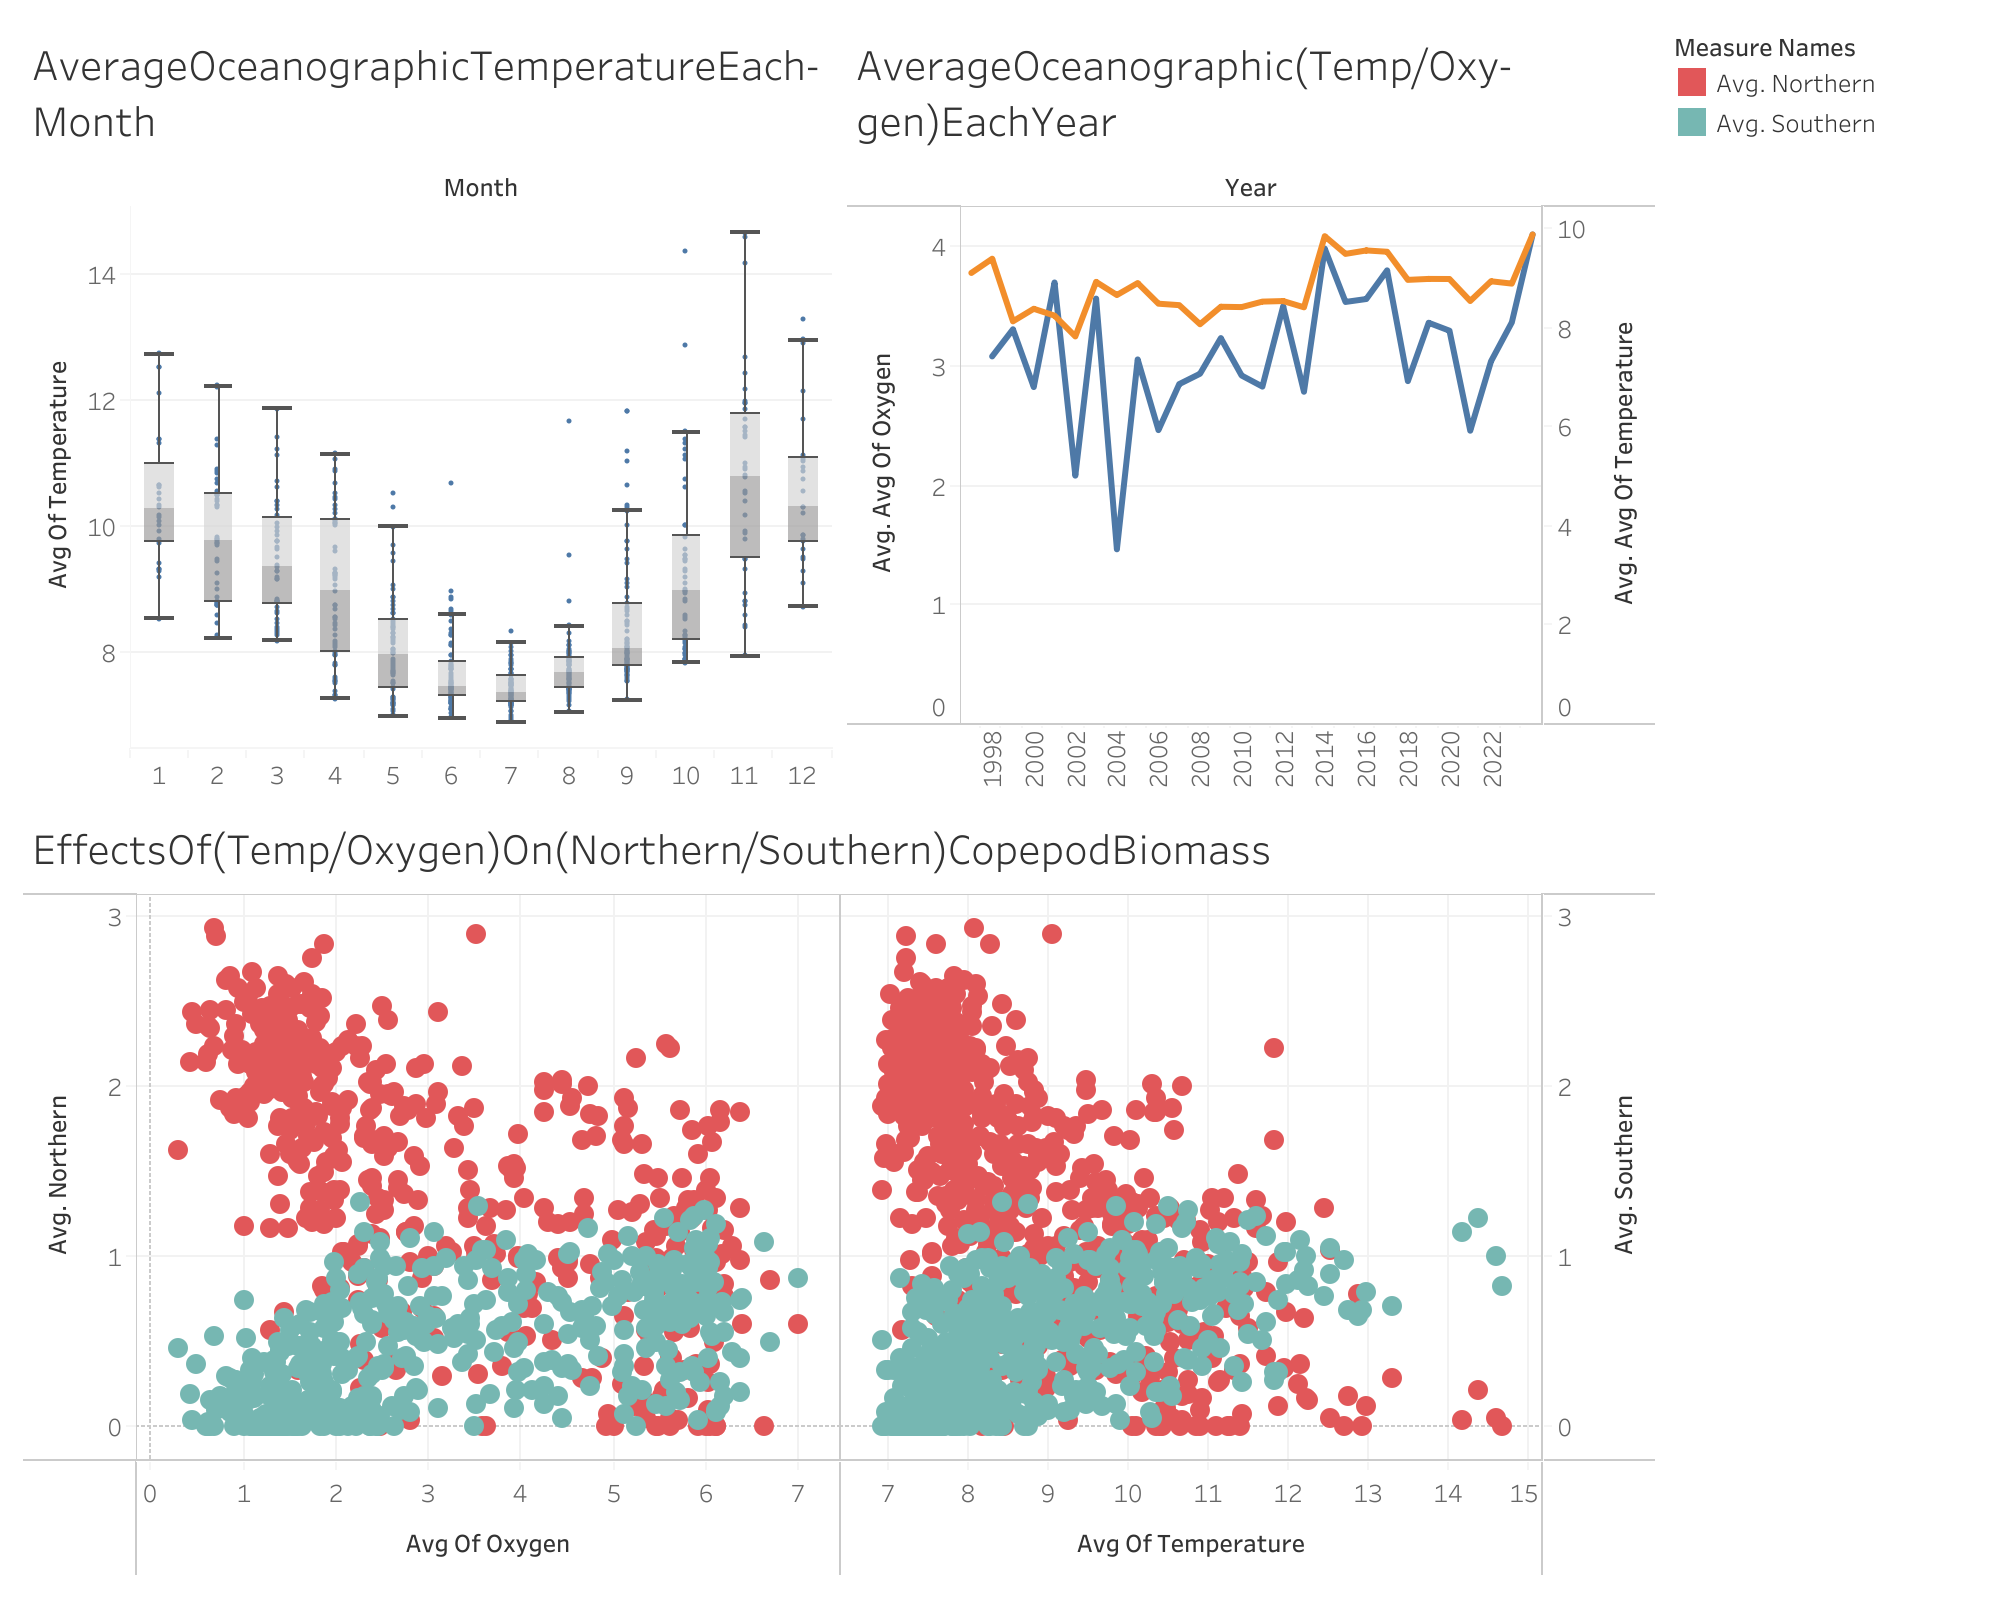
\includegraphics{NewportOceanographicDatasetDashboard.png}

The graph ``AverageOceanographicTemperatureEachMonth'' was a box plot
that measured the variables Avg of Temperature against the categorical
variable month. Each value of temperature that was sampled on its sample
date was recorded for each month. This graph shows how during the summer
months, the oceanographic temperature was lower than during the winter
months, differing from what would be commonly assumed.

The graph ``AverageOceanographic(Temp/Oxygen)EachYear'' was a dual axis
plot that measured the variables Avg of Temperature and Avg of Oxygen
against the categorical variable year. This plot shows the average
values of these two variables for each month so the viewer can see how
these values have changed throughout the years.

The graph ``EffectsOf(Temp/Oxygen)On(Northern/Southern)CopepodBiomass''
is a dual axis plot that measures four different variables. This plot
focuses on the effects that the oceanographic temperature and
oceanographic oxygen have on the population and copepod biomass recorded
on the sample dates and near the sample areas. From the graph, it is
visible that as oceanographic oxygen rises, the northern copepod biomass
greatly decreases and the southern copepod biomass slightly increases.
It is also evident that as oceanographic temperature rises, the northern
copepod biomass also greatly decreases and the southern copepod biomass
also slightly increases.

\subsection{Week 5}\label{week-5-1}

\section{Jupyter Notebooks}\label{jupyter-notebooks-1}

\subsection{Week 4}\label{week-4-1}

\begin{itemize}
\tightlist
\item
  \href{Tut2_Python_Pena_092024.ipynb}{Caleb's Notebook}: This notebook
  contains the data cleaning and exploration tasks.
\end{itemize}

\textbf{This is a markdown title}

In markdown, we can create lists:

\begin{itemize}
\tightlist
\item
  Item 1
\item
  Item 2
\item
  Item 3
\end{itemize}

We can also create enumerated lists:

\begin{enumerate}
\def\labelenumi{\arabic{enumi}.}
\tightlist
\item
  Hola
\item
  Hi
\item
  Namaste
\end{enumerate}

We can \textbf{bold} and \emph{italic}

\begin{Shaded}
\begin{Highlighting}[]
\CommentTok{\# Here we are importing numby with a nickname np}
\ImportTok{import}\NormalTok{ numpy }\ImportTok{as}\NormalTok{ np}
\BuiltInTok{print}\NormalTok{(np.absolute(}\OperatorTok{{-}}\DecValTok{1}\NormalTok{))}
\NormalTok{arr }\OperatorTok{=}\NormalTok{ np.array([}\DecValTok{1}\NormalTok{, }\DecValTok{2}\NormalTok{, }\DecValTok{3}\NormalTok{, }\DecValTok{4}\NormalTok{, }\DecValTok{5}\NormalTok{])}
\BuiltInTok{print}\NormalTok{(arr)}
\end{Highlighting}
\end{Shaded}

\begin{verbatim}
1
[1 2 3 4 5]
\end{verbatim}

\begin{Shaded}
\begin{Highlighting}[]
\CommentTok{\# Lists are native to Python}
\NormalTok{my\_list }\OperatorTok{=}\NormalTok{ [}\DecValTok{1}\NormalTok{, }\DecValTok{2}\NormalTok{, }\DecValTok{3}\NormalTok{, }\DecValTok{4}\NormalTok{, }\DecValTok{5}\NormalTok{]}
\BuiltInTok{print}\NormalTok{(my\_list)}
\end{Highlighting}
\end{Shaded}

\begin{verbatim}
[1, 2, 3, 4, 5]
\end{verbatim}

\begin{Shaded}
\begin{Highlighting}[]
\CommentTok{\# We will be using a lot of dataframes, so we need Pandas library}
\ImportTok{import}\NormalTok{ pandas }\ImportTok{as}\NormalTok{ pd}
\NormalTok{data }\OperatorTok{=}\NormalTok{ \{}\StringTok{\textquotesingle{}Ozone\textquotesingle{}}\NormalTok{: [}\DecValTok{41}\NormalTok{, }\DecValTok{36}\NormalTok{, }\DecValTok{12}\NormalTok{], }\StringTok{\textquotesingle{}Temp\textquotesingle{}}\NormalTok{: [}\DecValTok{67}\NormalTok{, }\DecValTok{72}\NormalTok{, }\DecValTok{74}\NormalTok{]\}}
\NormalTok{df }\OperatorTok{=}\NormalTok{ pd.DataFrame(data)}
\BuiltInTok{print}\NormalTok{(df)}
\end{Highlighting}
\end{Shaded}

\begin{verbatim}
   Ozone  Temp
0     41    67
1     36    72
2     12    74
\end{verbatim}

\textbf{4. Loading csv files}

To load .csv files into a \texttt{DataFrame}, we use the Pandas function
\texttt{read.csv}:

\begin{Shaded}
\begin{Highlighting}[]
\NormalTok{df }\OperatorTok{=}\NormalTok{ pd.read\_csv(}\StringTok{\textquotesingle{}airquality\_datasets.csv\textquotesingle{}}\NormalTok{)}
\end{Highlighting}
\end{Shaded}

\begin{Shaded}
\begin{Highlighting}[]
\BuiltInTok{print}\NormalTok{(df.info())}
\end{Highlighting}
\end{Shaded}

\begin{verbatim}
<class 'pandas.core.frame.DataFrame'>
RangeIndex: 153 entries, 0 to 152
Data columns (total 6 columns):
 #   Column   Non-Null Count  Dtype  
---  ------   --------------  -----  
 0   Ozone    116 non-null    float64
 1   Solar.R  146 non-null    float64
 2   Wind     153 non-null    float64
 3   Temp     153 non-null    int64  
 4   Month    153 non-null    int64  
 5   Day      153 non-null    int64  
dtypes: float64(3), int64(3)
memory usage: 7.3 KB
None
\end{verbatim}

\begin{Shaded}
\begin{Highlighting}[]
\BuiltInTok{print}\NormalTok{(df.describe())}
\end{Highlighting}
\end{Shaded}

\begin{verbatim}
            Ozone     Solar.R        Wind        Temp       Month         Day
count  116.000000  146.000000  153.000000  153.000000  153.000000  153.000000
mean    42.129310  185.931507    9.957516   77.882353    6.993464   15.803922
std     32.987885   90.058422    3.523001    9.465270    1.416522    8.864520
min      1.000000    7.000000    1.700000   56.000000    5.000000    1.000000
25%     18.000000  115.750000    7.400000   72.000000    6.000000    8.000000
50%     31.500000  205.000000    9.700000   79.000000    7.000000   16.000000
75%     63.250000  258.750000   11.500000   85.000000    8.000000   23.000000
max    168.000000  334.000000   20.700000   97.000000    9.000000   31.000000
\end{verbatim}

\textbf{5. Visualizing the Dataset}

Let's dive into visualizations using matplotlib. We'll start with simple
histograms and boxplots, then move on to correlation plots.

\textbf{Histograms} Histograms help us understand the distribution of
the variables. We'll create histograms for Ozone and Temp.

\begin{Shaded}
\begin{Highlighting}[]
\ImportTok{import}\NormalTok{ matplotlib.pyplot }\ImportTok{as}\NormalTok{ plt}

\CommentTok{\# Ozone Histogram}
\NormalTok{plt.figure(figsize}\OperatorTok{=}\NormalTok{(}\DecValTok{8}\NormalTok{, }\DecValTok{6}\NormalTok{))}
\NormalTok{plt.hist(df[}\StringTok{\textquotesingle{}Ozone\textquotesingle{}}\NormalTok{].dropna(), bins}\OperatorTok{=}\DecValTok{20}\NormalTok{, color}\OperatorTok{=}\StringTok{\textquotesingle{}blue\textquotesingle{}}\NormalTok{, edgecolor}\OperatorTok{=}\StringTok{\textquotesingle{}black\textquotesingle{}}\NormalTok{)}
\NormalTok{plt.title(}\StringTok{\textquotesingle{}Distribution of Ozone Levels\textquotesingle{}}\NormalTok{)}
\NormalTok{plt.xlabel(}\StringTok{\textquotesingle{}Ozone (ppb)\textquotesingle{}}\NormalTok{)}
\NormalTok{plt.ylabel(}\StringTok{\textquotesingle{}Frequency\textquotesingle{}}\NormalTok{)}
\NormalTok{plt.show()}
\end{Highlighting}
\end{Shaded}

\begin{verbatim}
Matplotlib is building the font cache; this may take a moment.
\end{verbatim}

\begin{figure}[H]

{\centering 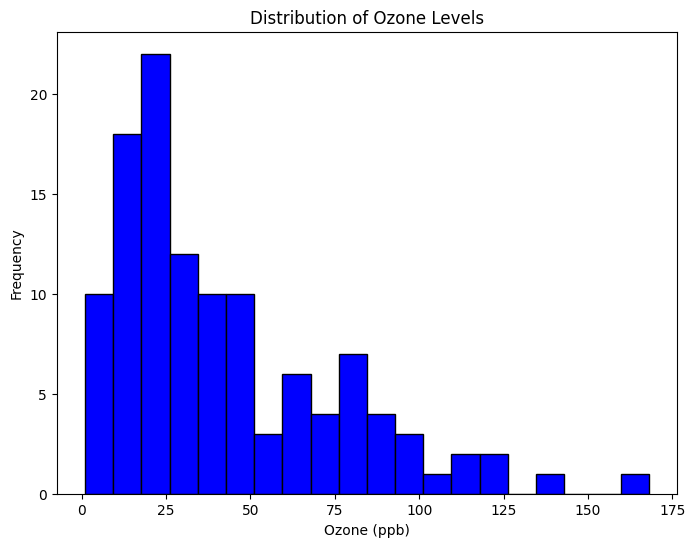
\includegraphics{Tut2_Python_Pena_092024_files/Tut2_Python_Pena_092024_9_1.png}

}

\caption{png}

\end{figure}%

\begin{Shaded}
\begin{Highlighting}[]
\CommentTok{\# Temp Histogram}
\NormalTok{plt.figure(figsize}\OperatorTok{=}\NormalTok{(}\DecValTok{8}\NormalTok{, }\DecValTok{6}\NormalTok{))}
\NormalTok{plt.hist(df[}\StringTok{\textquotesingle{}Temp\textquotesingle{}}\NormalTok{].dropna(), bins}\OperatorTok{=}\DecValTok{20}\NormalTok{, color}\OperatorTok{=}\StringTok{\textquotesingle{}orange\textquotesingle{}}\NormalTok{, edgecolor}\OperatorTok{=}\StringTok{\textquotesingle{}black\textquotesingle{}}\NormalTok{)}
\NormalTok{plt.title(}\StringTok{\textquotesingle{}Distribution of Temperature\textquotesingle{}}\NormalTok{)}
\NormalTok{plt.xlabel(}\StringTok{\textquotesingle{}Temperature (°F)\textquotesingle{}}\NormalTok{)}
\NormalTok{plt.ylabel(}\StringTok{\textquotesingle{}Frequency\textquotesingle{}}\NormalTok{)}
\NormalTok{plt.show()}
\end{Highlighting}
\end{Shaded}

\begin{figure}[H]

{\centering 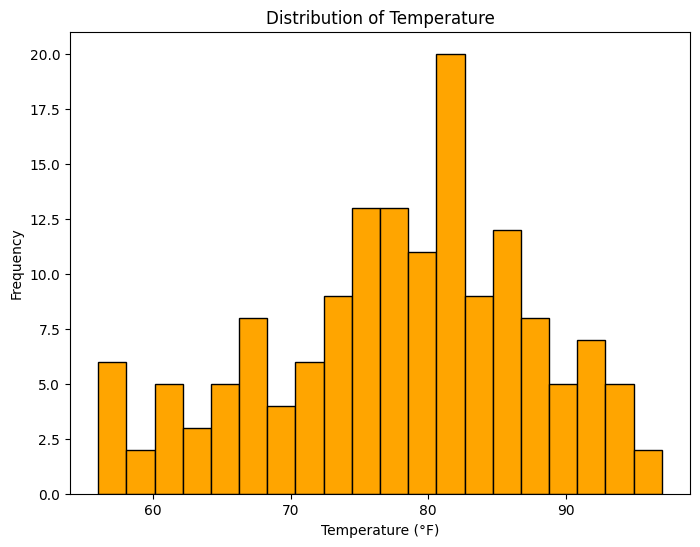
\includegraphics{Tut2_Python_Pena_092024_files/Tut2_Python_Pena_092024_10_0.png}

}

\caption{png}

\end{figure}%

\begin{Shaded}
\begin{Highlighting}[]

\end{Highlighting}
\end{Shaded}

\chapter{Derrick Baruga}\label{derrick-baruga}

This page contains all of Derrick Baruga's submissions this semester
organized into different sections.

\section{Wednesday}\label{wednesday-2}

\subsection{Week 1}\label{week-1-4}

\subsection{Week 2}\label{week-2-4}

I am using the air-quality dataset, which contains air quality
measurements collected over several months, specifically from May to
September. The dataset includes the following variables: \textbf{Ozone},
\textbf{Solar.R} (solar radiation), \textbf{Wind} (wind speed in miles
per hour), \textbf{Temp} (temperature in degrees Fahrenheit),
\textbf{Month} (ranging from 5 for May to 9 for September), and
\textbf{Day} (ranging from 1 to 31).

\textbf{Cleaning The Data}

I used Excel to clean the data by removing all rows with NA values and
performed an exploratory analysis to identify patterns, trends, and
potential relationships between these variables over the specified
months and days.

\textbf{Ozone Histogram}

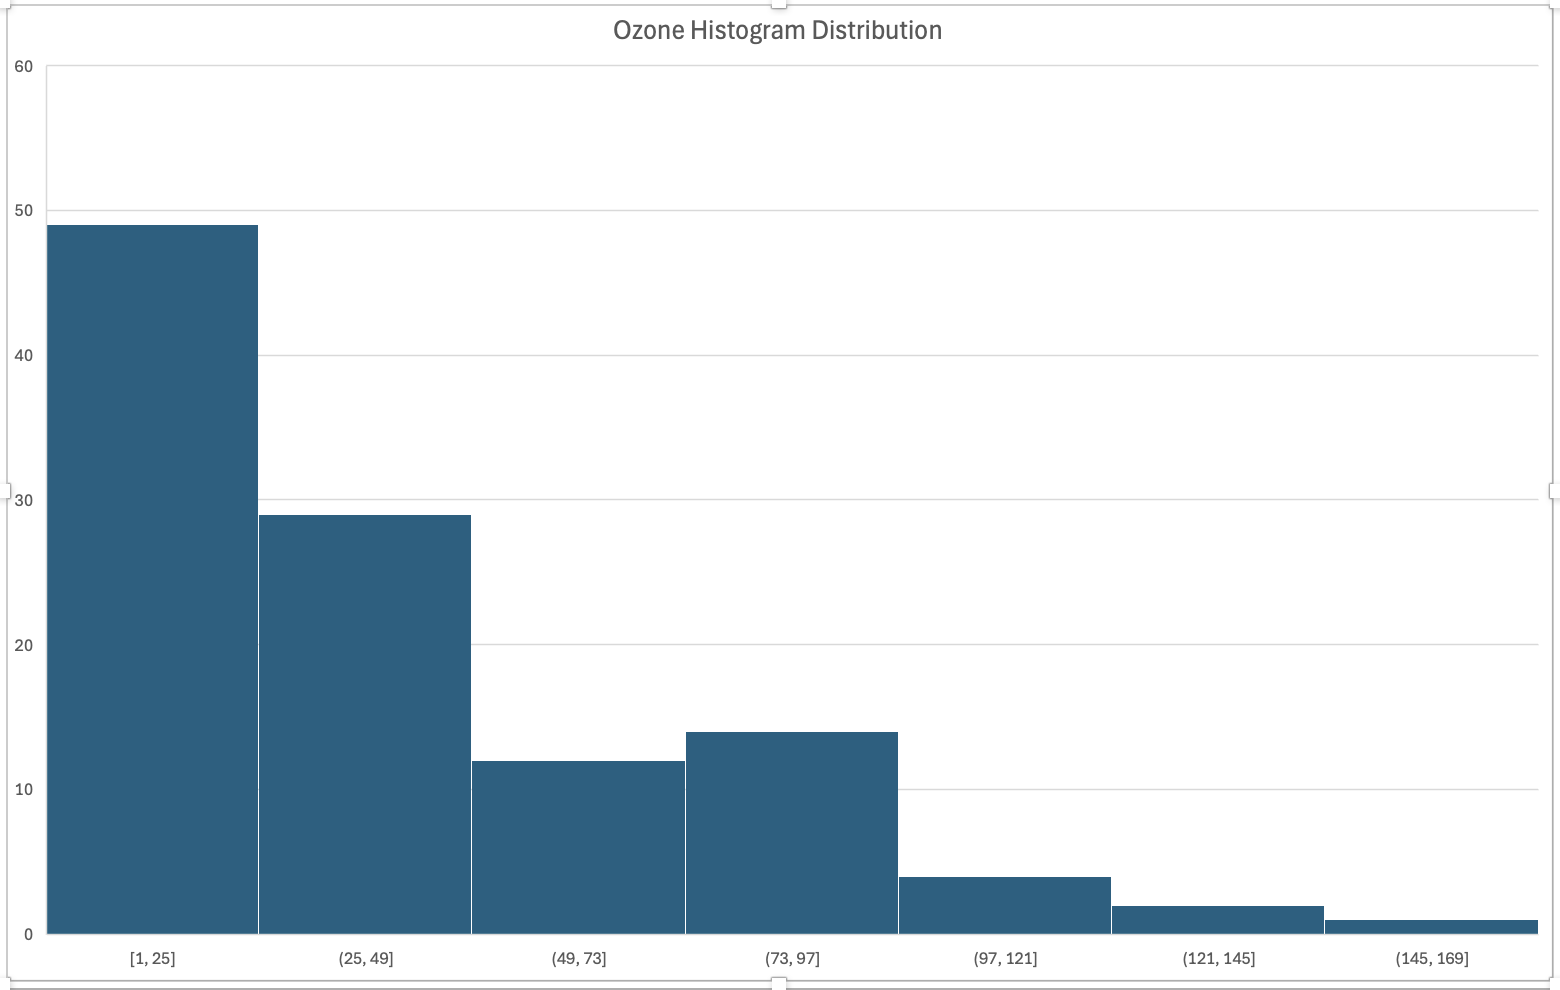
\includegraphics{hist_ozone_baruga.png}

The Ozone histogram has its highest values on the left and then curbs
off to the right, it indicates a right-skewed distribution.

This means:

\begin{itemize}
\tightlist
\item
  Most ozone values are low, with a few much higher values creating a
  long tail on the right.
\item
  The skewness could result from natural variability, pollution events,
  or weather conditions affecting ozone levels.
\end{itemize}

\textbf{Scatter Plot Ozone vs Temperature}

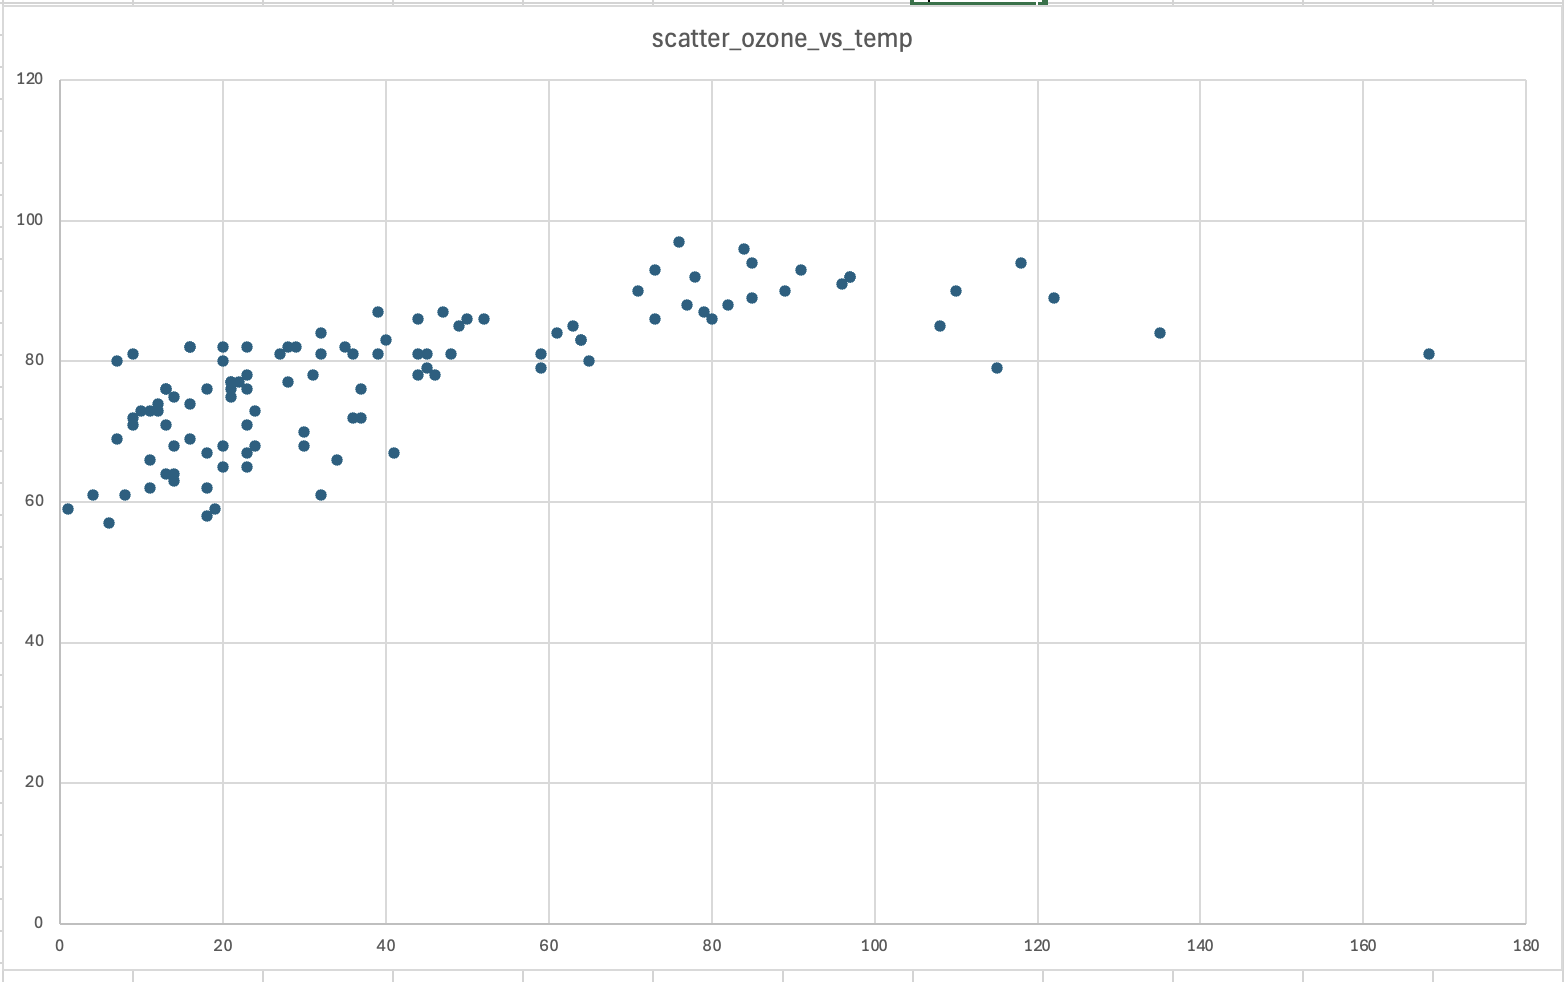
\includegraphics{scatter_ozone_vs_temp_baruga.png}

\begin{itemize}
\tightlist
\item
  A scatter plot of ozone (x-axis) vs.~temperature (y-axis) with a
  slight positive correlation means that higher ozone levels tend to be
  associated with higher temperatures. However, the relationship is
  weak, suggesting other factors (like wind, humidity, or pollution)
  also affect ozone levels and temperature.
\end{itemize}

\textbf{Pivot Table Average Ozones Per Day \& Month (Redacted)}

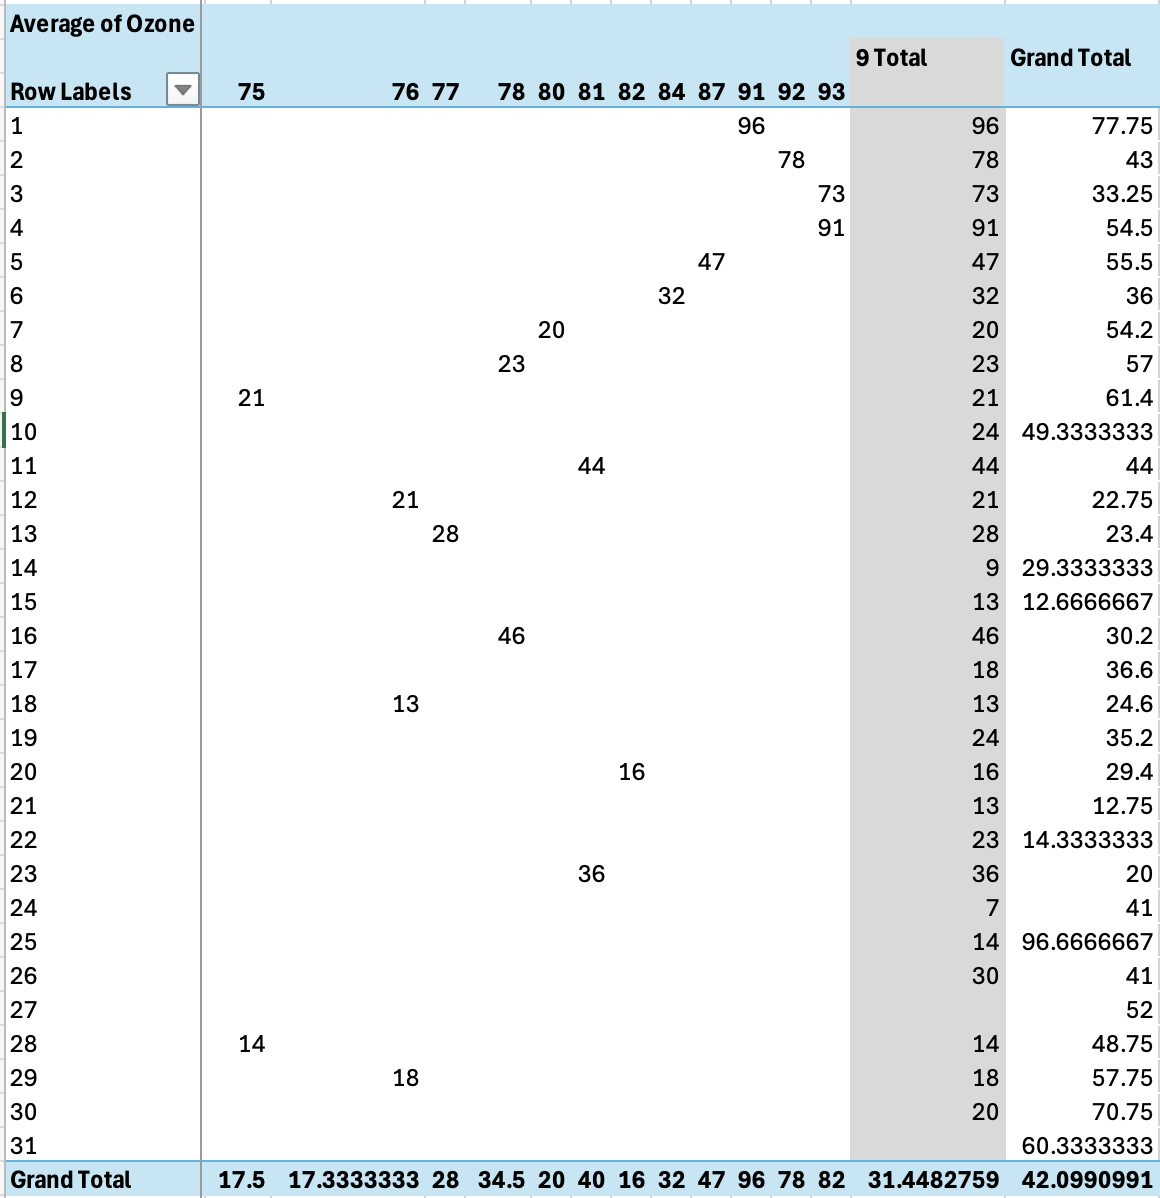
\includegraphics{pivot4_table_baruga.png}

\begin{itemize}
\tightlist
\item
  The pivot table presents daily sums for multiple variables
  (Temperature, Wind, Solar Radiation, and Ozone) over several months
  (May to September). The days with the highest ozone averages are Day
  25 in May (with an Ozone value of 5-65) and July (with an Ozone value
  of 7-74), with other notable days being Day 29 and Day 30 in May. The
  months with the highest ozone levels are May, which shows several days
  with high averages, and July, particularly on Days 25 and 29.
\end{itemize}

\textbf{Pivot Chart Average Ozones Per Day \& Month}

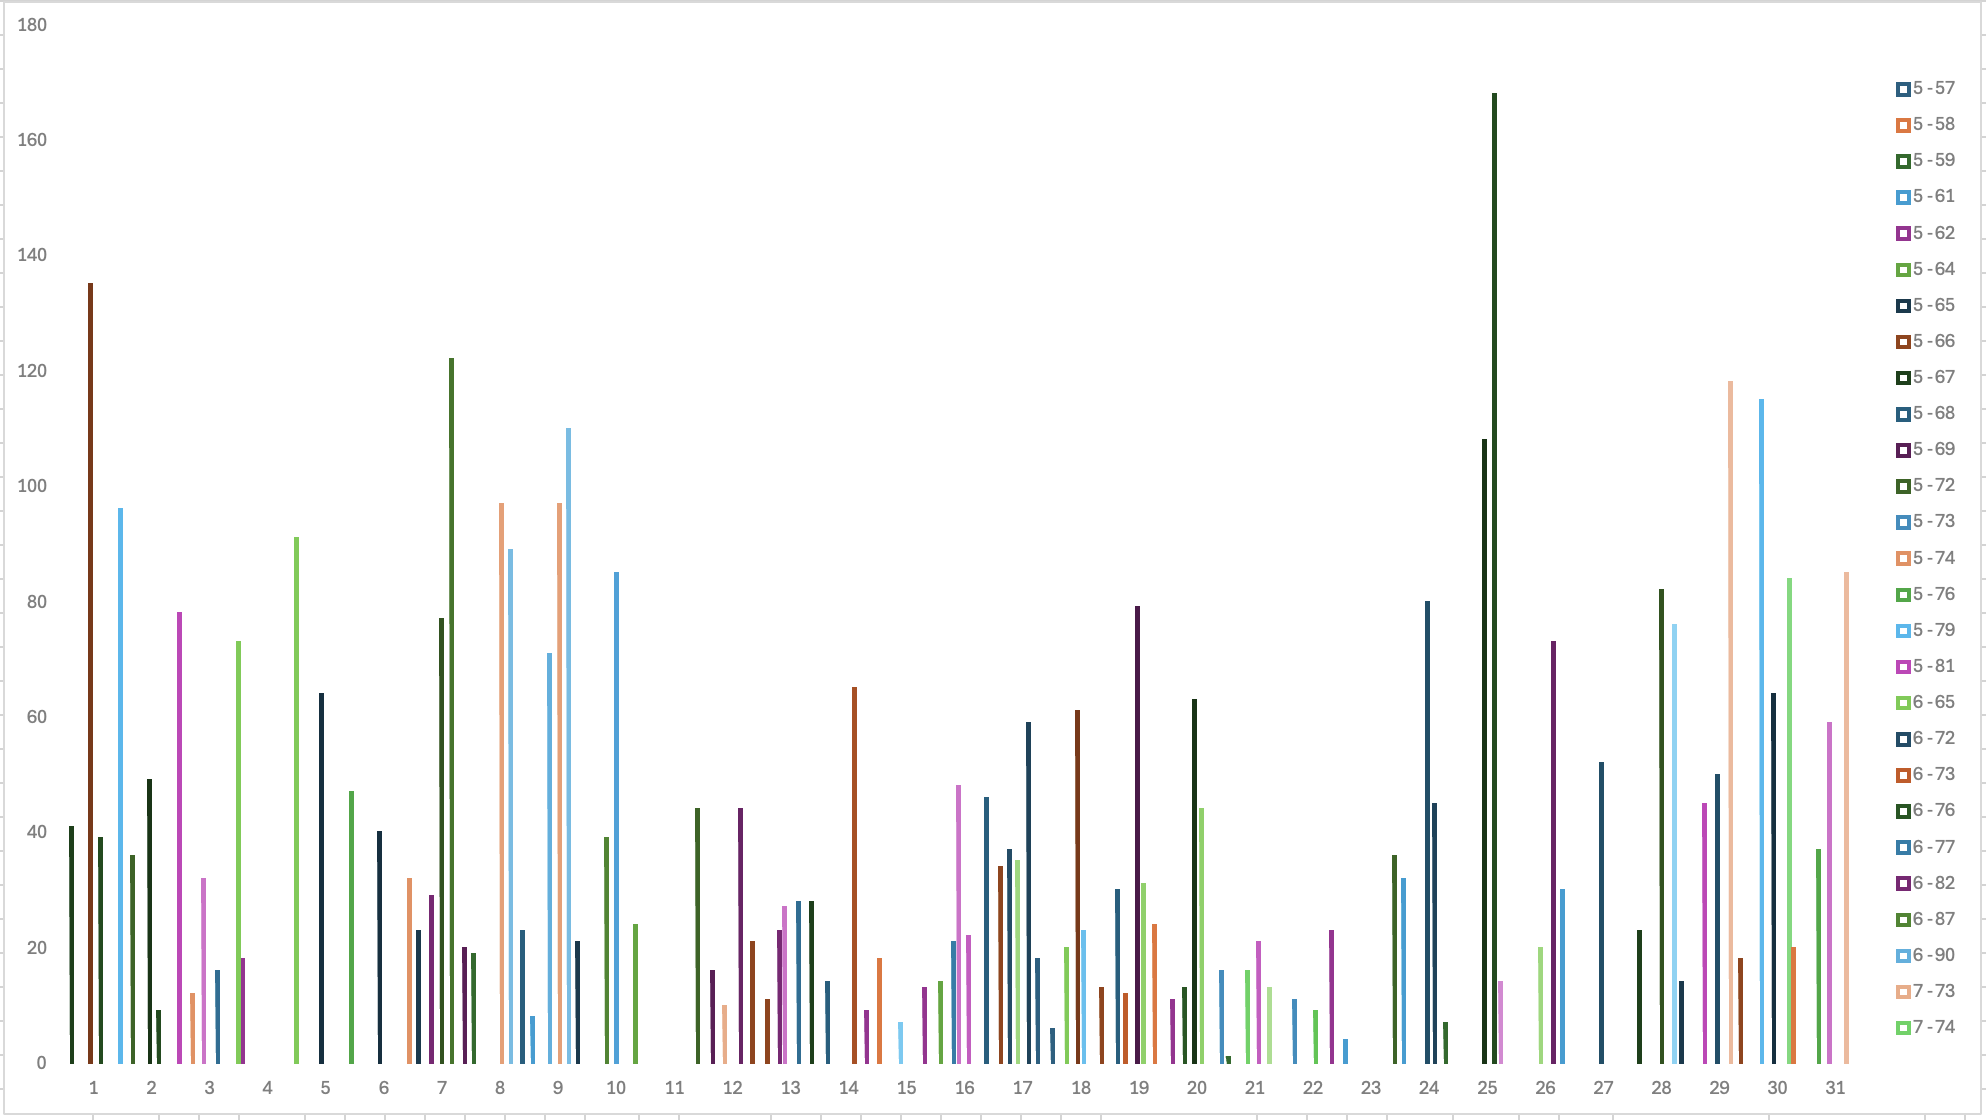
\includegraphics{pivot4_chart_baruga.png}

\textbf{Pivot Table of Variation in Solar Radiation and Temperature}

\begin{itemize}
\tightlist
\item
  The pivot chart provide a visual representation of how these variables
  change over time. The histogram shows day-to-day variations in ozone
  levels, with the highest concentrations occurring in the summer
  months. Notably, there is a pronounced peak around July 25th,
  indicating exceptionally high ozone levels on that day. May and July
  both have elevated levels, with smaller peaks around May 29th and
  30th, but July 25th stands out as the most significant. Overall, the
  chart confirms that ozone levels are highest in July, particularly
  around the 25th.
\end{itemize}

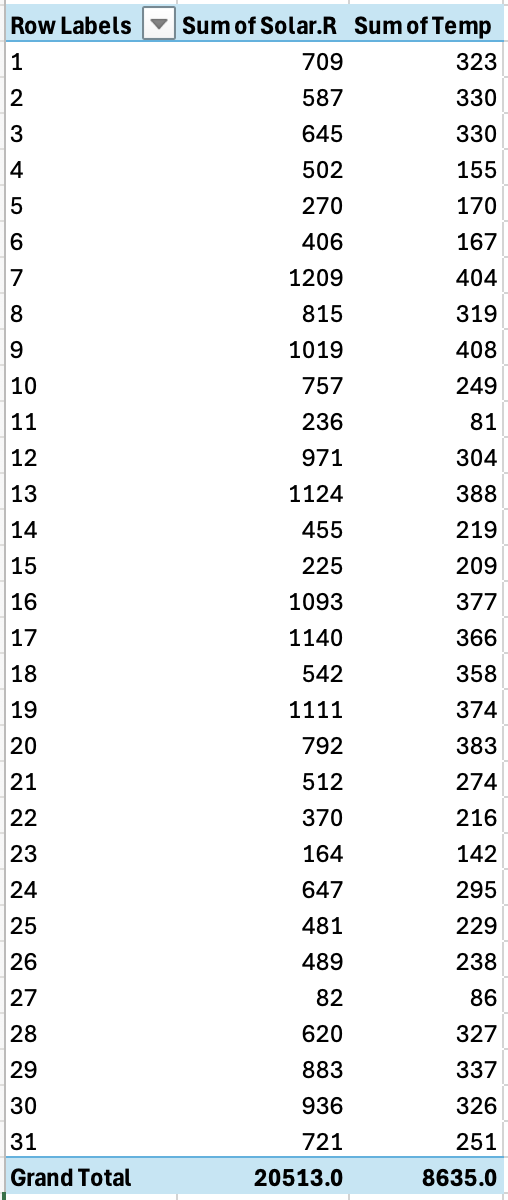
\includegraphics{pivot1_table_baruga.png}

\begin{itemize}
\tightlist
\item
  The pivot table shows daily sums for Solar Radiation and Temperature
  over a month. There is noticeable daily variation, with high values on
  days like 18, 19, and 29, indicating intense sunlight and warmer
  temperatures, and lower values on days like 23 and 27, reflecting
  cooler conditions. The grand totals summarize the entire month, with
  20,513 for Solar Radiation and 8,635 for Temperature. Overall, the
  table captures daily fluctuations in weather conditions.
\end{itemize}

** Pivot Chart of Pivot Chart of Variation in Solar Radiation and
Temperature**

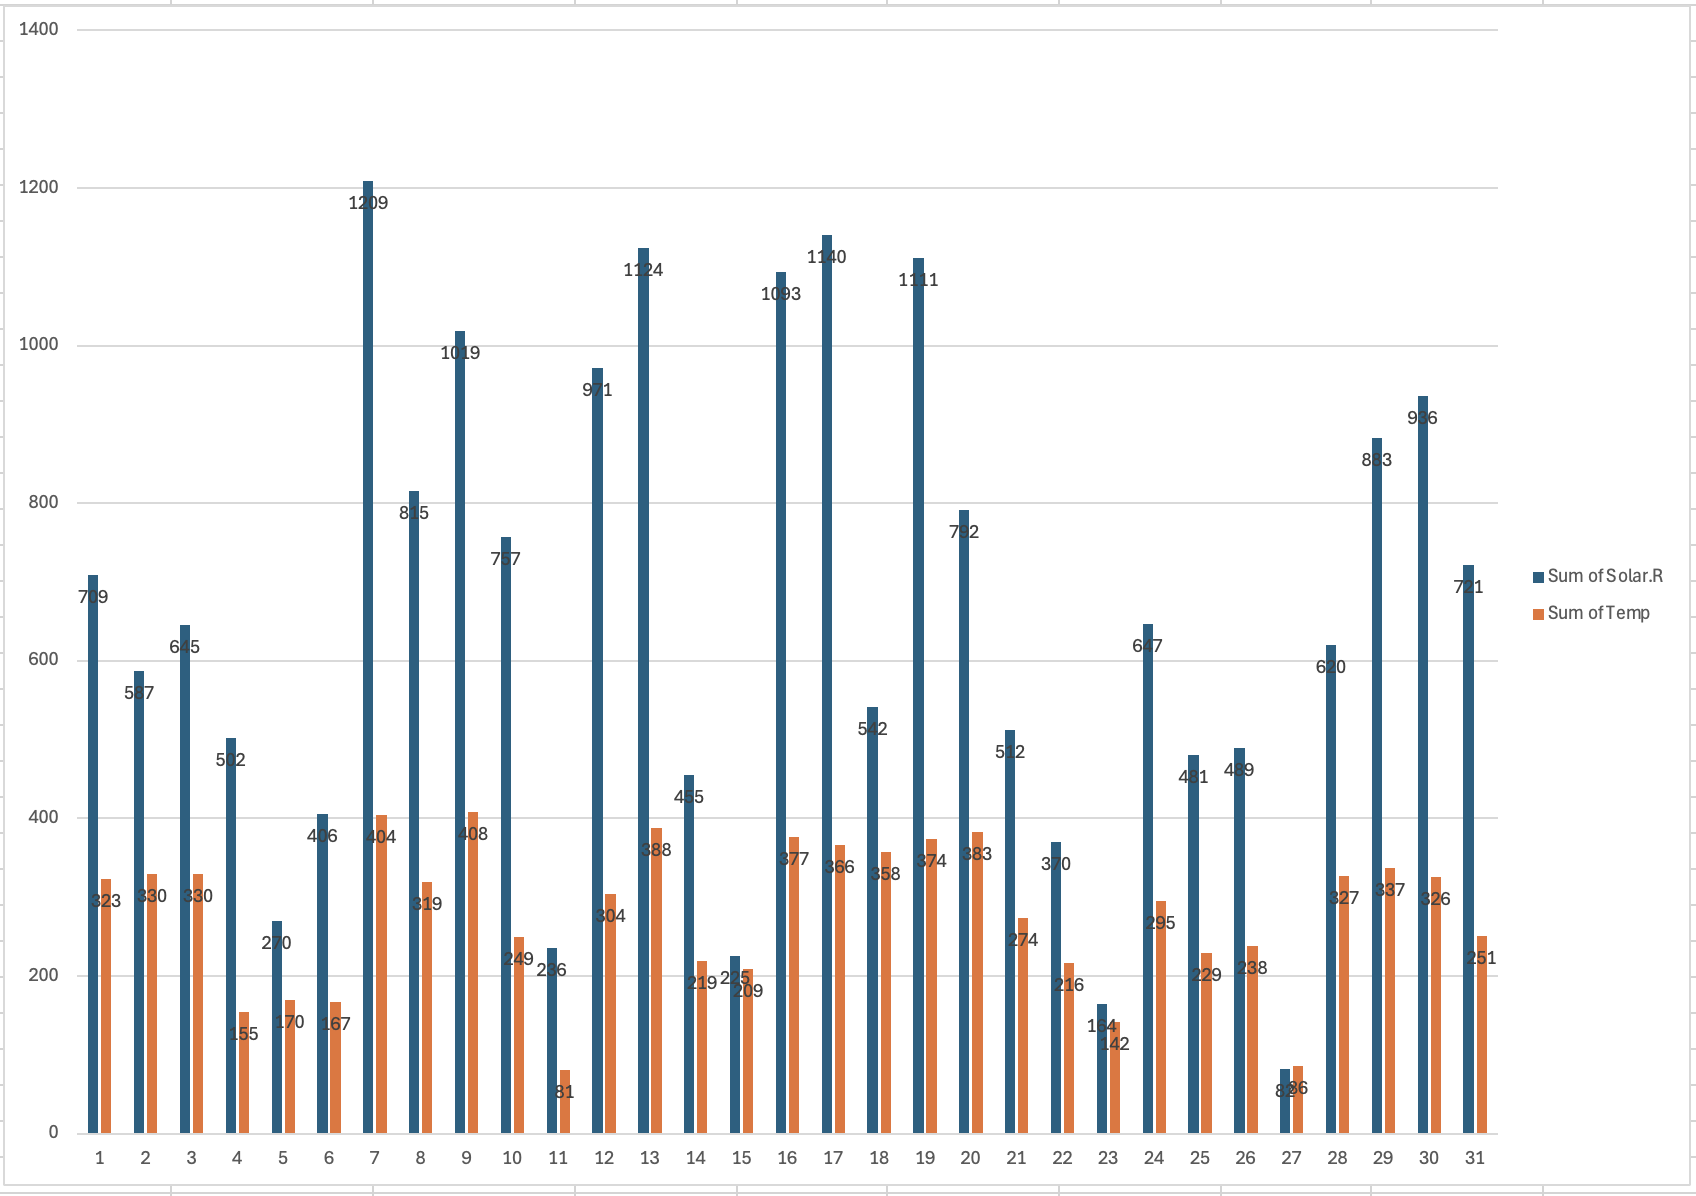
\includegraphics{pivot1_chart_baruga.png}

\begin{itemize}
\tightlist
\item
  The bar chart shows daily sums of Solar Radiation (blue) and
  Temperature (orange) over 31 days. High Solar Radiation is notable on
  days like 9, 13, 16, 18, 19, and 29, with values exceeding 1,000.
  Temperature values are generally lower, mostly below 400, with higher
  values on days like 9 and 18. There are significant day-to-day
  variations, with some days showing high Solar Radiation but lower
  temperatures (e.g., Day 13). The chart captures daily fluctuations and
  highlights days with extreme values.
\end{itemize}

\textbf{Pivot Table}

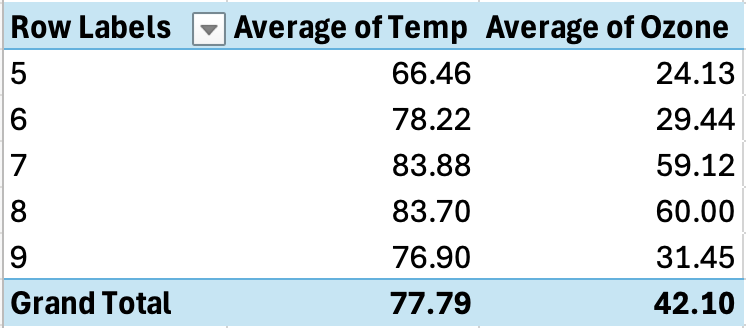
\includegraphics{pivot2_table_baruga.png}

\begin{itemize}
\tightlist
\item
  The pivot table displays the average temperature
  (\texttt{Average\ of\ Temp}) and ozone levels
  (\texttt{Average\ of\ Ozone}) for days labeled 5 to 9, showing average
  temperatures ranging from 66.46 to 83.88, with the highest
  temperatures recorded on days 7 and 8. Ozone levels vary
  significantly, from a low of 24.13 on Day 5 to a high of 60.00 on Day
  8. Overall, the average temperature for the period is 77.79, and the
  average ozone level is 42.10, reflecting moderate temperatures with
  variable ozone levels across these days and highlighting daily
  fluctuations in both metrics.
\end{itemize}

\textbf{Pivot Chart}

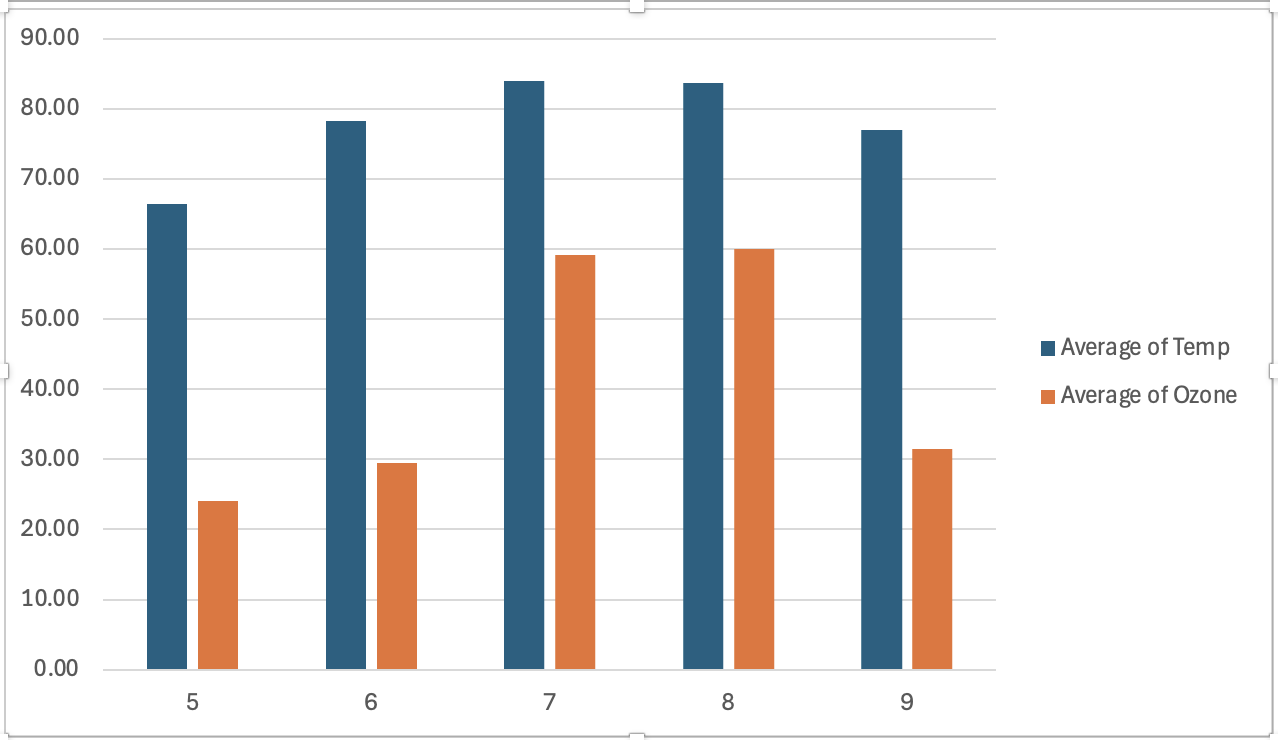
\includegraphics{pivot2_chart_baruga.png}

\begin{itemize}
\tightlist
\item
  The bar chart illustrates the average temperature (in blue) and
  average ozone levels (in orange) for days 5 to 9, showing that
  temperatures remain relatively high throughout, ranging from around 66
  on Day 5 to approximately 84 on Days 7 and 8. Ozone levels start low
  on Day 5 (around 24), rise significantly by Days 7 and 8 (around
  59-60), and then decrease slightly on Day 9 (around 31). The chart
  suggests a potential correlation between higher temperatures and
  elevated ozone levels, as Days 7 and 8, which have the highest
  temperatures, also show the highest average ozone levels, indicating
  noticeable variability over the period.
\end{itemize}

\subsection{Week 3}\label{week-3-2}

\href{https://public.tableau.com/views/Book1_17262574551960/Dashboard1?:language=en-US&publish=yes&:sid=&:redirect=auth&:display_count=n&:origin=viz_share_link}{Wednesday
Dashboard}

\begin{enumerate}
\def\labelenumi{\arabic{enumi}.}
\tightlist
\item
  \textbf{Histogram of Avg REM Sleep}:
\end{enumerate}

\begin{itemize}
\item
  This bar chart shows the average REM sleep time categorized by both
  conservation status (like ``cd,'' ``en,'' ``lc'') and dietary habits
  (carnivore, herbivore, omnivore, etc.).
\item
  The distribution indicates variations in REM sleep depending on these
  factors. For example, certain categories, such as carnivores with an
  ``lc'' (least concern) conservation status, seem to have higher
  average REM sleep.
\end{itemize}

\begin{enumerate}
\def\labelenumi{\arabic{enumi}.}
\setcounter{enumi}{1}
\tightlist
\item
  \textbf{Stacked Bar Chart of Vore vs.~REM Sleep}:
\end{enumerate}

\begin{itemize}
\item
  This chart displays the breakdown of average REM sleep across
  different dietary categories and their conservation statuses, further
  subdivided by animal order.
\item
  It provides detailed insights into how sleep patterns differ based on
  dietary habits and animal groups. For instance, ``Carnivora'' under
  different conservation statuses like ``lc'' and ``domesticated'' shows
  varying REM sleep levels.
\end{itemize}

\begin{enumerate}
\def\labelenumi{\arabic{enumi}.}
\setcounter{enumi}{2}
\tightlist
\item
  \textbf{Packed Bubble Chart of Order}:
\end{enumerate}

\begin{itemize}
\item
  The chart uses bubbles to represent different orders of animals, with
  the size of each bubble possibly corresponding to the number of
  species or the average REM sleep within that order.
\item
  Colors differentiate various dietary habits (``vore''), showing how
  different animal orders fall into categories such as carnivores,
  herbivores, omnivores, etc.
\end{itemize}

\begin{enumerate}
\def\labelenumi{\arabic{enumi}.}
\setcounter{enumi}{3}
\tightlist
\item
  \textbf{Treemap of Order}:
\end{enumerate}

\begin{itemize}
\item
  This chart breaks down the animal orders into smaller rectangles,
  where the size of each rectangle may indicate the average REM sleep,
  the number of species, or another quantitative measure.
\item
  The colors correspond to different orders, offering a visual overview
  of how these orders compare in the measured metric.
\end{itemize}

\section{Friday - Midterm Projects}\label{friday---midterm-projects-2}

\subsection{Week 1}\label{week-1-5}

\subsection{Week 2}\label{week-2-5}

title: ``Midterm\_Project\_Baruga'' subtitle: ``Data.gov: Warehouse and
Retail Sales'' format: html ---

\textbf{Context of the Dataset}

\begin{itemize}
\tightlist
\item
  \textbf{Title}: Warehouse and Retail Sales
\item
  \textbf{Link}:
  \href{https://data.montgomerycountymd.gov/api/views/v76h-r7br/rows.csv?accessType=DOWNLOAD}{Download
  the CSV dataset}
\end{itemize}

The \emph{Warehouse and Retail Sales} dataset provides a comprehensive
view of sales activities in Montgomery County, Maryland, by capturing
data from various warehouse and retail operations. This dataset was
collected through a combination of direct reporting from businesses,
automated sales tracking systems, and regional sales surveys. The data
encompasses a range of sales metrics, including volume and product
categories, to offer insights into business performance across different
types of establishments.

The dataset includes the following variables:

\begin{itemize}
\tightlist
\item
  Row Labels: Categories or identifiers used to organize and classify
  the sales data.
\item
  BEER: Sales volume for beer products.
\item
  DUNNAGE: Sales volume for dunnage products, which are materials used
  to protect goods during transportation.
\item
  KEGS: Sales volume for kegs, typically used for storing and
  transporting beverages.
\item
  LIQUOR: Sales volume for liquor products.
\item
  NON-ALCOHOL: Sales volume for non-alcoholic beverages.
\item
  REF: Sales volume for refrigeration supplies or products.
\item
  STR\_SUPPLIES: Sales volume for store supplies, which may include
  various retail essentials.
\item
  WINE: Sales volume for wine products.
\item
  Grand Total: The total sales volume across all categories combined.
\end{itemize}

** Data Cleaning and Preparation**

\begin{enumerate}
\def\labelenumi{\arabic{enumi}.}
\tightlist
\item
  \textbf{Import the Data}: I downloaded and loaded the CSV file into
  Excel.
\item
  \textbf{Check for Missing Values}: My preferred method for handling
  NAs is by highlighting them and deselecting them using the filter tool
  for each column as I feel most thorough by doing that. Using the
  following steps ``Select the entire dataset, go to Home \textgreater{}
  Conditional Formatting \textgreater{} Highlight Cells Rules
  \textgreater{} Blanks to highlight all blank cells.''
\item
  \textbf{Data Formatting}: Formated any columns that need specific data
  types (such as dates as date format, numbers as currency or
  percentage).
\end{enumerate}

\begin{itemize}
\tightlist
\item
  Specifically I used the =TEXTJOIN(``-'', TRUE, A2, B2) function to
  join column one (YYYY) and column two (MM) into a new column called
  TIME
\end{itemize}

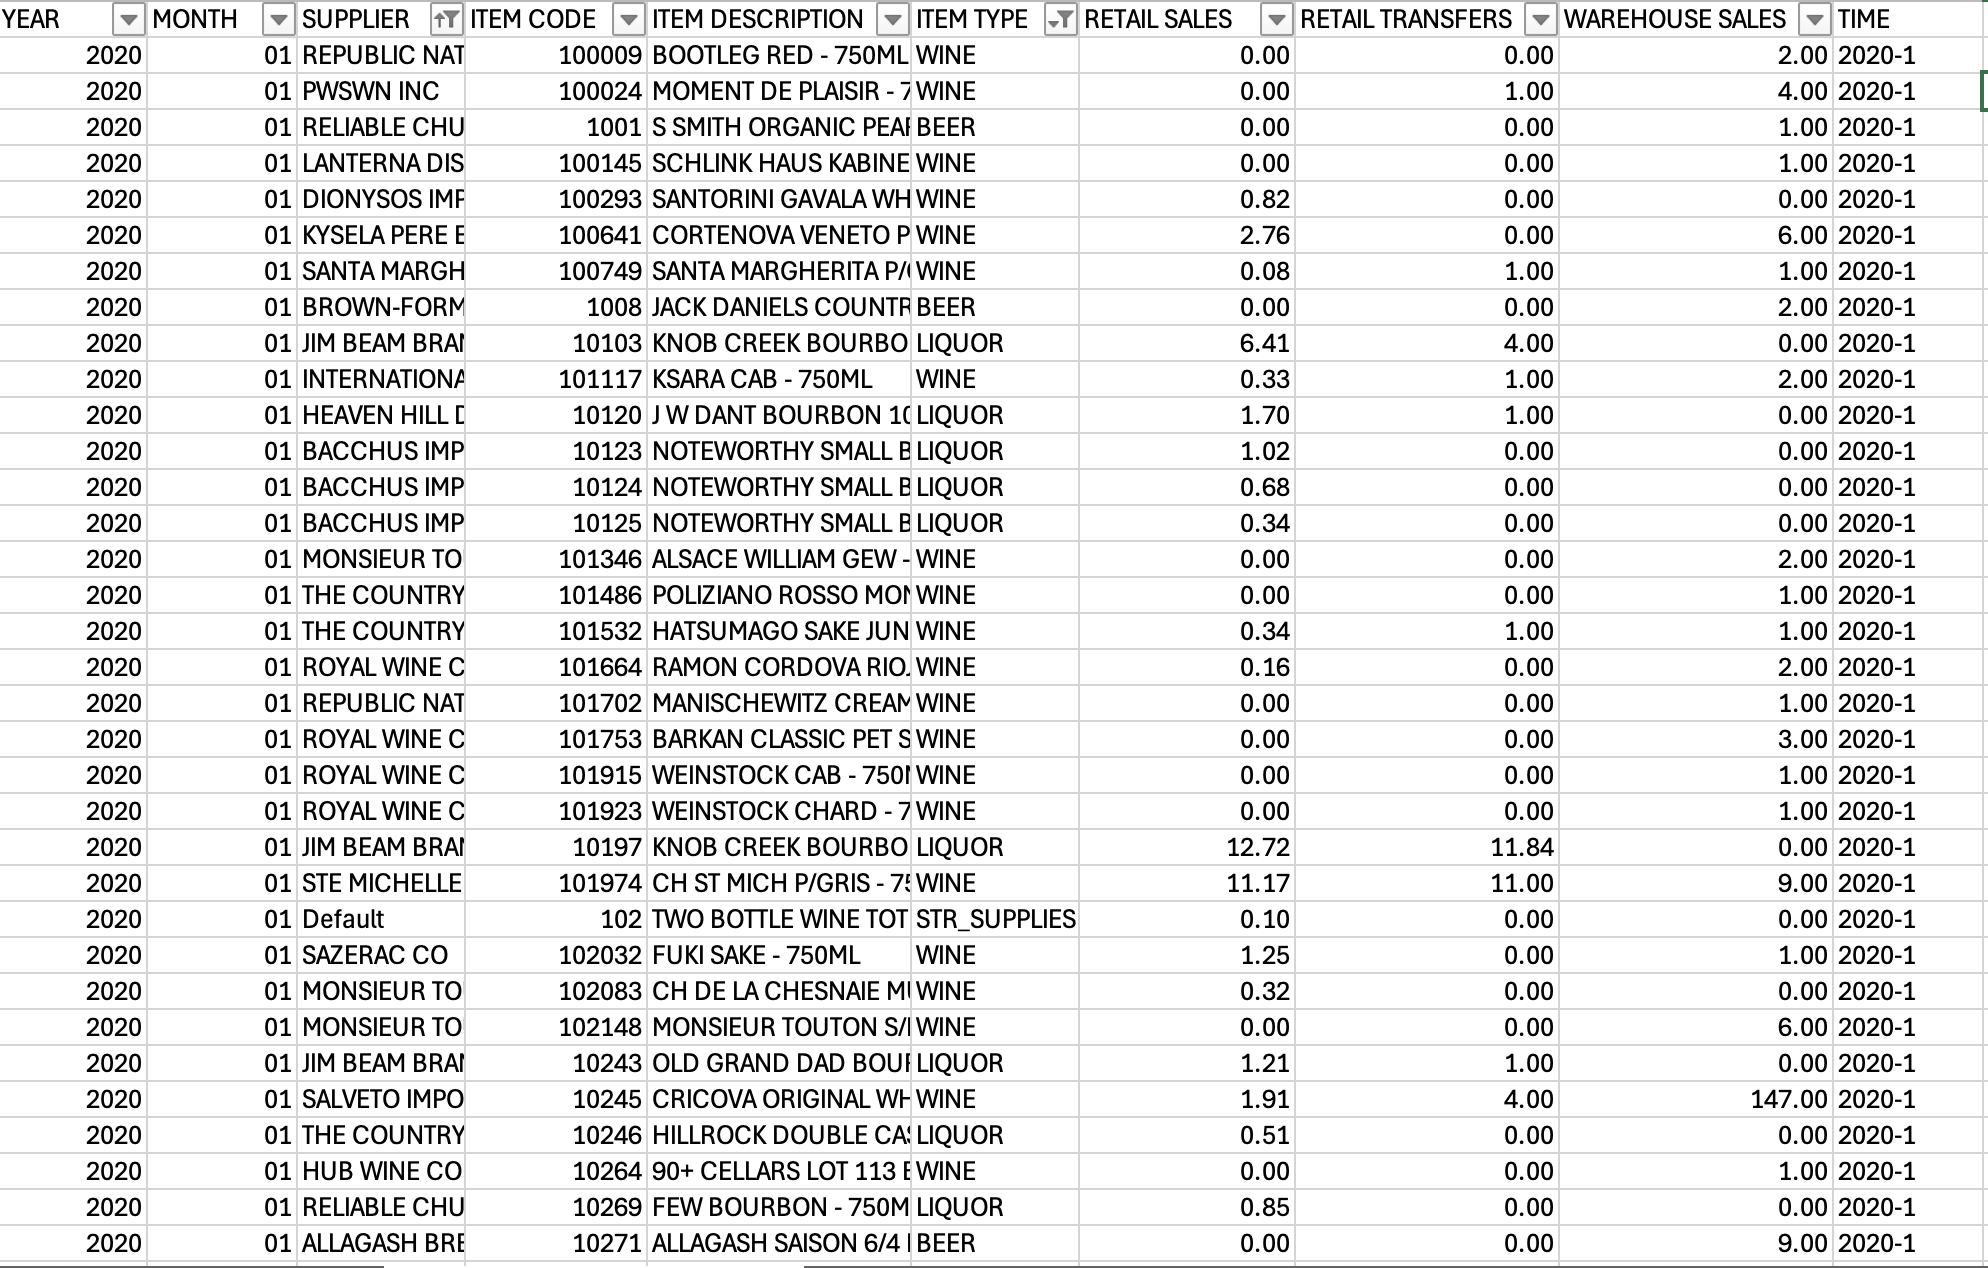
\includegraphics{summary_screenshot.png}

\textbf{Visualization}

\textbf{Pivot Tables YT link:}
https://www.youtube.com/watch?v=qu-AK0Hv0b4

\begin{itemize}
\tightlist
\item
  Pivot tables are a powerful and user friendly (drag and drop) summary
  statistic/visualisation tool that I used to get an intial feel of my
  data.
\end{itemize}

Here are the findings:

\textbf{Warehouse Sales/Expenses of Beverages Over Time (2017 - 2020)}

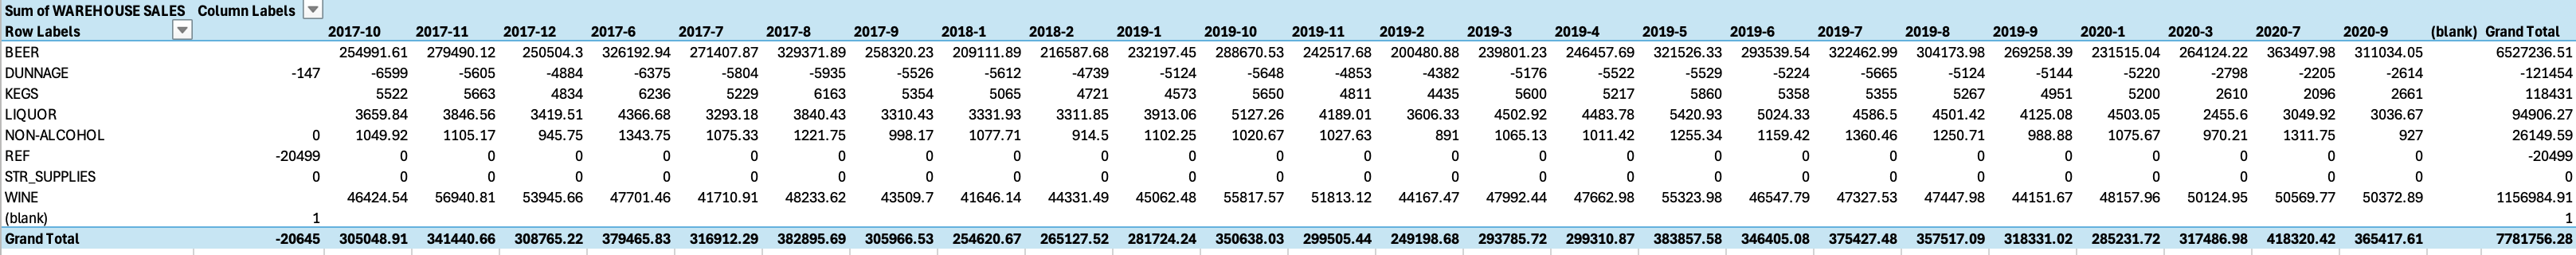
\includegraphics{pivot_table_baruga.png}

\begin{itemize}
\tightlist
\item
  \textbf{Overall Sales}: \textbf{\emph{BEER}} has the highest sales,
  followed by \textbf{\emph{WINE}}, while \textbf{\emph{DUNNAGE}},
  \textbf{\emph{REF}}, and \textbf{\emph{STR\_SUPPLIES}} have negative
  or minimal sales, which makes sense as refers to materials used to
  protect goods during shipping and handling, such as packing materials
  or cushioning, and as such is an expense to the business leading to
  its negative output on revenue.
\item
  \textbf{Monthly Trends}: \textbf{\emph{BEER}} sales vary
  significantly, with large peaks and drops. \textbf{\emph{WINE}} sales
  are more stable but still show some fluctuation. \textbf{\emph{KEGS}}
  and \textbf{\emph{LIQUOR}} show positive but lower sales.
\end{itemize}

\textbf{Histogram of Warehouse Sales/Expenses of Beverages Over Time}

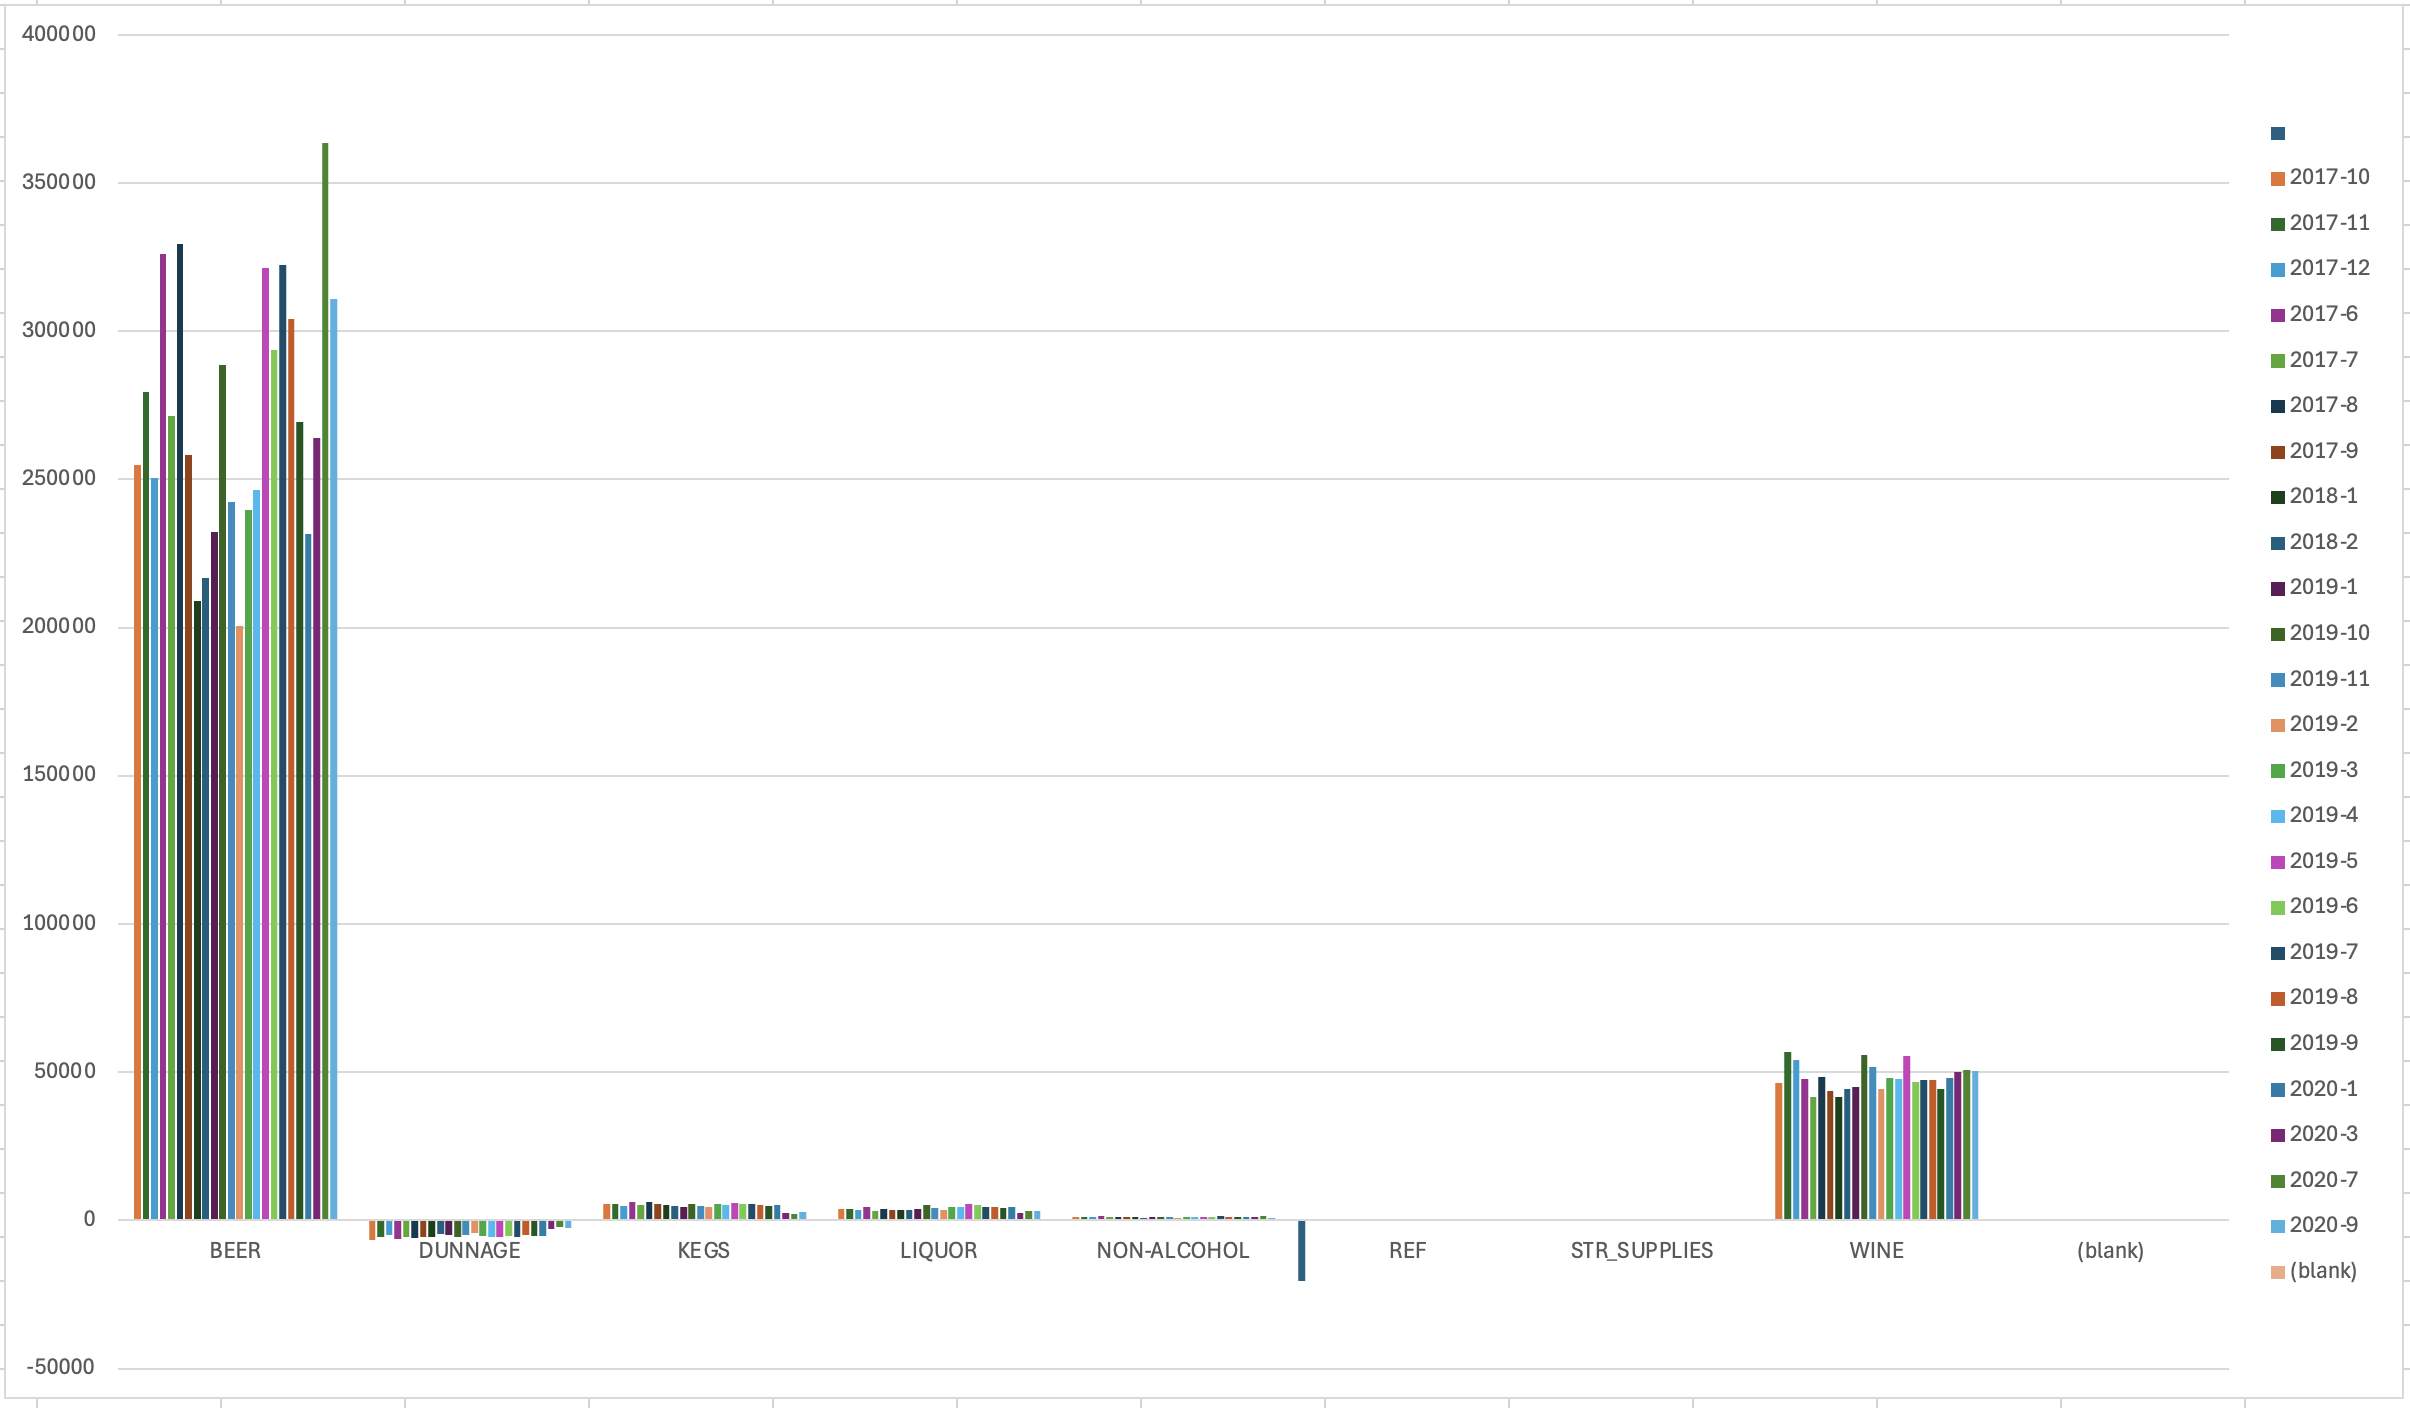
\includegraphics{pivot_chart.png}

\begin{itemize}
\tightlist
\item
  Here is a histogram representation of the aforementioned summary pivot
  tables. There appears to be a disporportionate amount of
  \textbf{\emph{BEER}} bought for warehouses. But that could be due to
  the fact that beers are sold in packs and so single unit quantity has
  skyrocketed in order to make a ``12 pack'' that will later count as
  one unit sold at retail.
\end{itemize}

\textbf{Retail Sales of Beverages Over Time (2017 - 2020)}

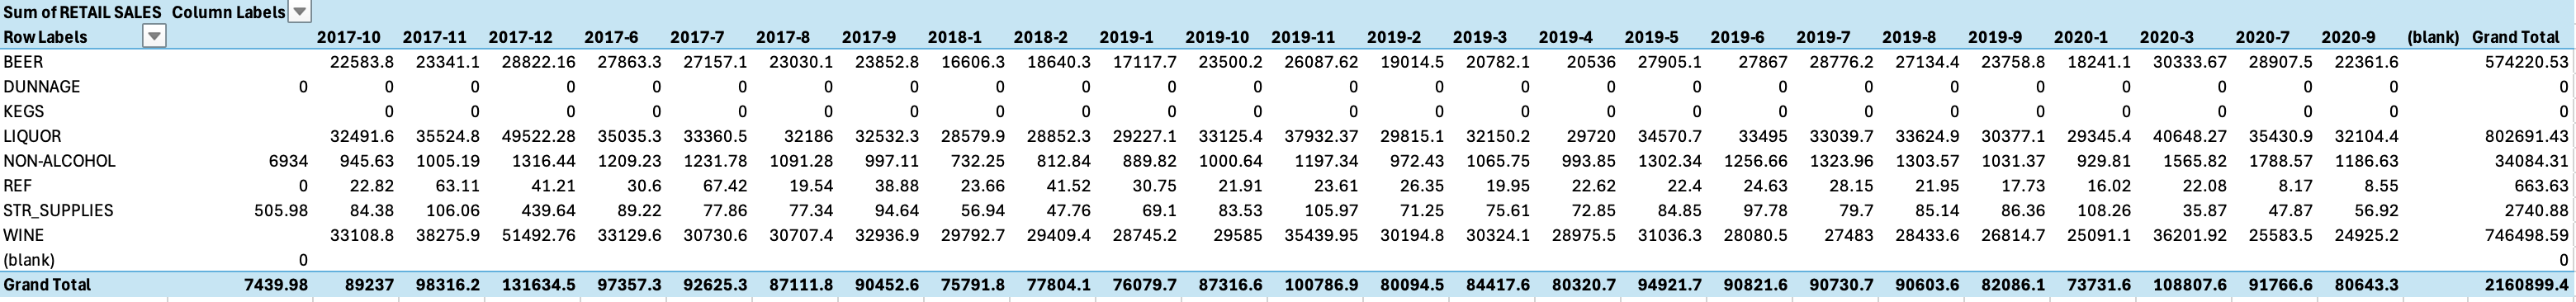
\includegraphics{pivot2_table.png}

\begin{itemize}
\tightlist
\item
  \textbf{Product Types}: Includes Beer, Liquor, Wine, Non-Alcoholic
  beverages, and others, with substantial sales figures for Beer,
  Liquor, and Wine.
\item
  \textbf{Sales Trends}: Liquor leads with \$802,691.43 in total sales,
  followed by Wine (\$746,498.59) and Beer (\$574,220.53). Recent months
  show higher sales for Beer and Wine.
\item
  \textbf{Low Sales Categories}: Items like Dunnage and Kegs have
  negligible or zero sales.
\item
  \textbf{Overall Total}: Total sales across all products amount to
  \$2,160,899.37, highlighting overall retail activity.
\end{itemize}

\textbf{Histogram of Retail Sales of Beverages Over Time}

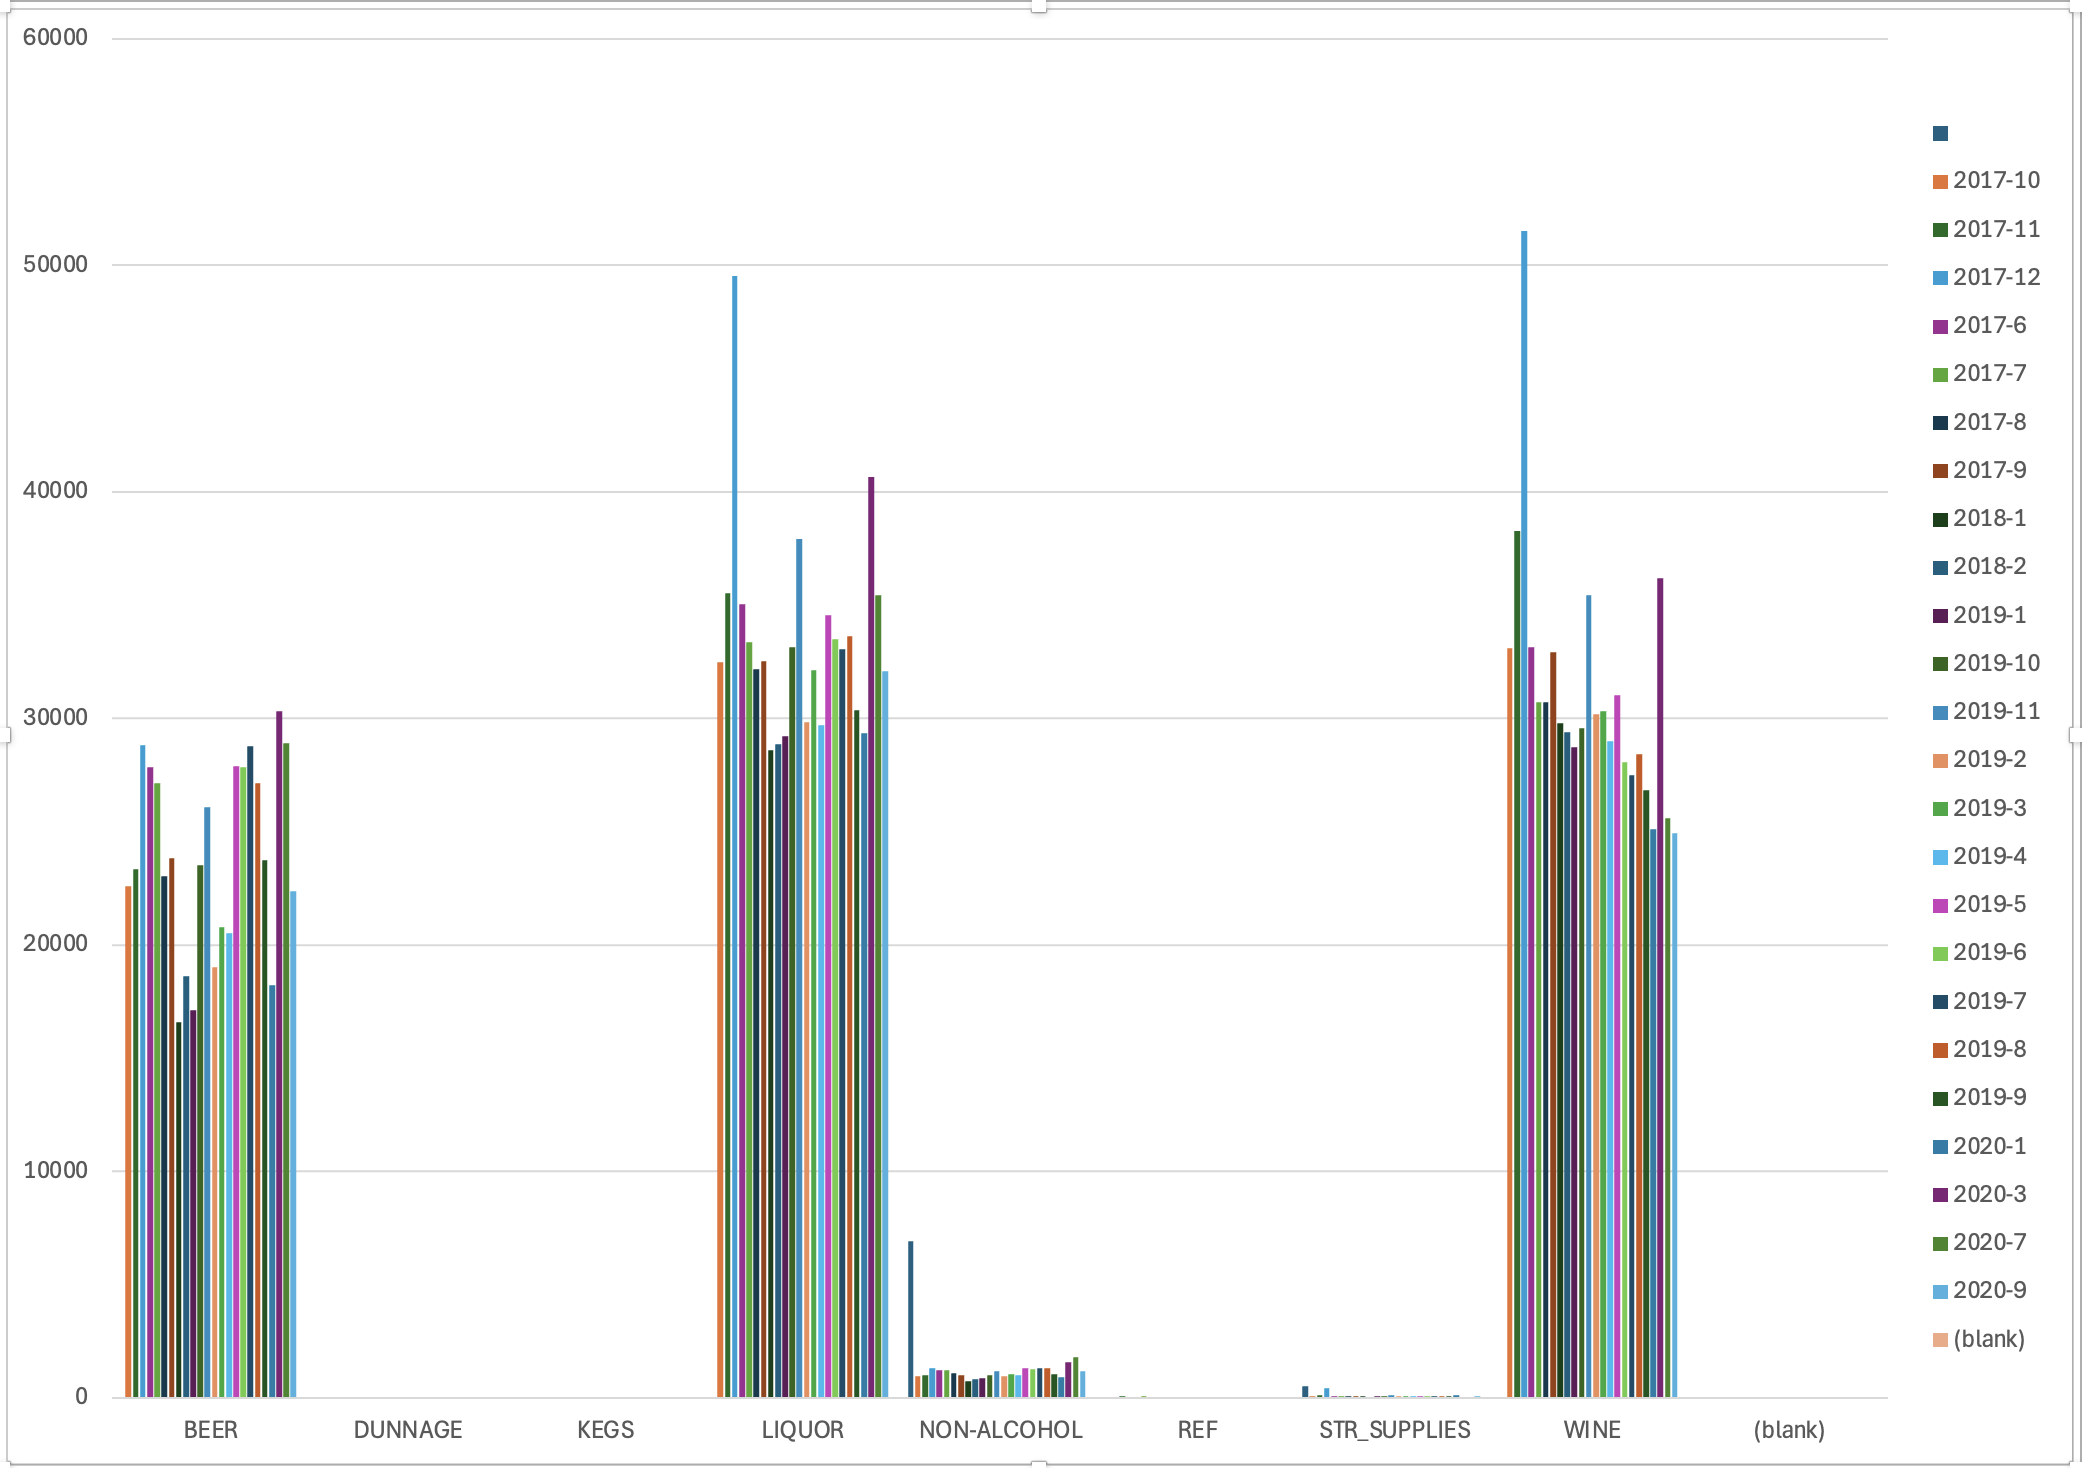
\includegraphics{pivot_chart_2.png}

\begin{itemize}
\tightlist
\item
  Once we come to the retail side of things we see that
  \textbf{\emph{WINE}} and \textbf{\emph{LIQUOR}} are clear best
  sellers. It is shown hower that \textbf{\emph{LIQUOR}} has begun to
  overtake \textbf{\emph{WINE}} in retail sales.
\end{itemize}

\textbf{Summary}

From the ``Warehouse and Retail Sales'' dataset, I found that Beer leads
in warehouse sales, with notable fluctuations due to bulk packaging,
while Wine and Liquor have more stable sales. Retail sales show Liquor
as the top seller, recently surpassing Wine, with Beer also performing
strongly but declining. The histograms illustrate high Beer volume in
warehouses and a shift in retail dominance from Wine to Liquor. Next, I
will analyze seasonal trends, create advanced visualizations for deeper
insights, and finalize the report with comprehensive findings and
recommendations. \#\#\# Week 2 \#\#\# Week 3

\subsection{Week 3}\label{week-3-3}

\href{https://public.tableau.com/views/Book1_17262574551960/Dashboard2?:language=en-US&publish=yes&:sid=&:redirect=auth&:display_count=n&:origin=viz_share_link}{Wednesday
Dashboard}

\textbf{1.Histogram of Avg Sales Over Time:}

\begin{itemize}
\item
  This stacked bar chart displays the average retail sales from June
  2017 to September 2020, broken down by different item types such as
  ``BEER,'' ``WINE,'' ``LIQUOR,'' ``NON-ALCOHOL,'' and others.
\item
  The chart shows monthly fluctuations in sales, with noticeable peaks
  around December 2017 and July 2020. This suggests seasonal effects or
  particular periods of high demand for certain items.
\item
  The different colors represent various item types, indicating the
  contribution of each category to the total sales in each month. For
  example, ``LIQUOR'' and ``NON-ALCOHOL'' seem to contribute
  significantly to the total sales during peak months.
\end{itemize}

\textbf{2. Area Chart: Avg Sales vs.~Transfers:}

\begin{itemize}
\item
  This plot consists of two layered area charts: the top one shows
  average retail transfers, and the bottom one shows average retail
  sales over the same period (June 2017 to September 2020).
\item
  Both charts use colors to represent different item types, revealing
  how each type contributes to overall sales and transfers.
\item
  The charts indicate that the trends in transfers often align with the
  sales trends, which suggests a correlation between the quantity of
  goods transferred and the sales performance.
\item
  Peaks and troughs in the charts could indicate seasonal variations,
  inventory management strategies, or market demand shifts for various
  items.
\end{itemize}

\textbf{3. Packed Bubble Chart of Avg Sales Over Time:}

\begin{itemize}
\item
  This chart visualizes average sales using bubbles, where the size of
  each bubble reflects the volume of sales, and the color represents
  different item types.
\item
  Larger bubbles correspond to higher sales, indicating which item types
  have the greatest impact on sales over time.
\item
  The variety of bubble sizes and colors reveals the diversity in item
  types and their varying sales performance.
\end{itemize}

\textbf{4. Treemap of Retail Transfers vs.~Retail Sales:}

\begin{itemize}
\item
  The treemap displays retail sales data, with each rectangle
  representing different categories (``NON-ALCOHOL,'' ``BEER,''
  ``LIQUOR,'' ``REF,'' etc.) and specific years (2017, 2019, 2020).
\item
  The size of each rectangle corresponds to the magnitude of sales, and
  the color shading indicates the average retail sales, with darker
  shades representing higher sales.
\item
  This visualization shows how different item types and their sales vary
  in significance. For example, ``NON-ALCOHOL'' items appear to have a
  prominent share, especially in 2020.
\end{itemize}

\subsection{Week 8}\label{week-8-1}

This contains Derrick Week 8 Submissions

I chose the dataset ``Federal, State, and Local Government
Transportation-Related Revenues and Expenditures, Fiscal Year'' provides
financial data on transportation-related revenues and expenditures
across federal, state, and local governments in the United States,
measured in millions of current dollars. It includes detailed
information on government revenues from user charges and taxes
specifically allocated for transportation programs, as well as
expenditures in this sector over multiple fiscal years. The dataset
excludes general fund revenues and borrowing proceeds, focusing on
own-source revenues.

The data is sourced from the U.S. Department of Transportation's Bureau
of Transportation Statistics (BTS) and is published under the National
Transportation Statistics Table 3-29, available on the BTS website. This
dataset is instrumental for analyzing transportation funding and
government spending trends at various governmental levels.

\textbf{Dataset Exploration}

\begin{Shaded}
\begin{Highlighting}[]
\CommentTok{\# Load necessary libraries}
\FunctionTok{library}\NormalTok{(readxl)  }\CommentTok{\# To read Excel files}
\FunctionTok{library}\NormalTok{(dplyr)   }\CommentTok{\# For data manipulation}
\end{Highlighting}
\end{Shaded}

\begin{verbatim}

Attaching package: 'dplyr'
\end{verbatim}

\begin{verbatim}
The following objects are masked from 'package:stats':

    filter, lag
\end{verbatim}

\begin{verbatim}
The following objects are masked from 'package:base':

    intersect, setdiff, setequal, union
\end{verbatim}

\begin{Shaded}
\begin{Highlighting}[]
\FunctionTok{library}\NormalTok{(ggplot2) }\CommentTok{\# For visualization}
\end{Highlighting}
\end{Shaded}

\begin{verbatim}
Warning: package 'ggplot2' was built under R version 4.3.2
\end{verbatim}

\begin{Shaded}
\begin{Highlighting}[]
\CommentTok{\# Task 1: Load the dataset}
\NormalTok{file\_path }\OtherTok{\textless{}{-}}  \StringTok{"C:/Users/toluf/OneDrive/Desktop/Dynamic 2/Archive 2/table\_03\_29\_061324.xlsx"} 


\NormalTok{dataset }\OtherTok{\textless{}{-}} \FunctionTok{read\_excel}\NormalTok{(file\_path, }\AttributeTok{sheet =} \DecValTok{2}\NormalTok{)}
\end{Highlighting}
\end{Shaded}

\begin{verbatim}
New names:
* `` -> `...2`
* `` -> `...3`
* `` -> `...4`
* `` -> `...5`
* `` -> `...6`
* `` -> `...7`
* `` -> `...8`
* `` -> `...9`
* `` -> `...10`
* `` -> `...11`
* `` -> `...12`
* `` -> `...13`
* `` -> `...14`
* `` -> `...15`
* `` -> `...16`
\end{verbatim}

\begin{Shaded}
\begin{Highlighting}[]
\CommentTok{\# Explore the structure of the dataset}
\FunctionTok{str}\NormalTok{(dataset)}
\end{Highlighting}
\end{Shaded}

\begin{verbatim}
tibble [17 x 16] (S3: tbl_df/tbl/data.frame)
 $ Table 3-29:  Federal, State, and Local Government Transportation-Related Revenues and Expenditures, Fiscal Year (millions of current dollars): chr [1:17] NA "Total government revenues" "Federal" "State and local" ...
 $ ...2                                                                                                                                         : num [1:17] 2007 163884 53967 109917 268843 ...
 $ ...3                                                                                                                                         : num [1:17] 2008 163222 52102 111120 284343 ...
 $ ...4                                                                                                                                         : num [1:17] 2009 157684 47287 110397 300267 ...
 $ ...5                                                                                                                                         : num [1:17] 2010 160472 47244 113227 303516 ...
 $ ...6                                                                                                                                         : num [1:17] 2011 171324 50310 121014 303784 ...
 $ ...7                                                                                                                                         : num [1:17] 2012 179173 54473 124699 314024 ...
 $ ...8                                                                                                                                         : num [1:17] 2013 174527 50686 123841 309276 ...
 $ ...9                                                                                                                                         : num [1:17] 2014 183537 54161 129376 324000 ...
 $ ...10                                                                                                                                        : num [1:17] 2015 194195 56714 137481 329551 ...
 $ ...11                                                                                                                                        : num [1:17] 2016 194420 57279 137141 339439 ...
 $ ...12                                                                                                                                        : num [1:17] 2017 203528 57628 145900 355374 ...
 $ ...13                                                                                                                                        : num [1:17] 2018 213373 60035 153338 370884 ...
 $ ...14                                                                                                                                        : num [1:17] 2019 228293 62142 166150 384211 ...
 $ ...15                                                                                                                                        : num [1:17] 2020 200560 53719 146842 404177 ...
 $ ...16                                                                                                                                        : num [1:17] 2021 196163 53503 142660 398764 ...
\end{verbatim}

\begin{Shaded}
\begin{Highlighting}[]
\CommentTok{\# Check for missing values}
\FunctionTok{summary}\NormalTok{(dataset)}
\end{Highlighting}
\end{Shaded}

\begin{verbatim}
 Table 3-29:  Federal, State, and Local Government Transportation-Related Revenues and Expenditures, Fiscal Year (millions of current dollars)
 Length:17                                                                                                                                    
 Class :character                                                                                                                             
 Mode  :character                                                                                                                             
                                                                                                                                              
                                                                                                                                              
                                                                                                                                              
                                                                                                                                              
      ...2             ...3             ...4             ...5       
 Min.   :  2007   Min.   :  2008   Min.   :  2009   Min.   :  2010  
 1st Qu.: 42052   1st Qu.: 45088   1st Qu.: 42913   1st Qu.: 43445  
 Median : 81942   Median : 81611   Median : 82167   Median : 85120  
 Mean   :114380   Mean   :118497   Mean   :121481   Mean   :123375  
 3rd Qu.:183756   3rd Qu.:186542   3rd Qu.:185882   3rd Qu.:188221  
 Max.   :268843   Max.   :284343   Max.   :300267   Max.   :303516  
 NA's   :9        NA's   :9        NA's   :9        NA's   :9       
      ...6             ...7             ...8             ...9       
 Min.   :  2011   Min.   :  2012   Min.   :  2013   Min.   :  2014  
 1st Qu.: 46028   1st Qu.: 49049   1st Qu.: 46068   1st Qu.: 48811  
 Median : 87711   Median : 91481   Median : 90561   Median : 94066  
 Mean   :125829   Mean   :130834   Mean   :128363   Mean   :134480  
 3rd Qu.:196144   3rd Qu.:204692   3rd Qu.:200162   3rd Qu.:210463  
 Max.   :303784   Max.   :314024   Max.   :309276   Max.   :324000  
 NA's   :9        NA's   :9        NA's   :9        NA's   :9       
     ...10            ...11            ...12            ...13       
 Min.   :  2015   Min.   :  2016   Min.   :  2017   Min.   :  2018  
 1st Qu.: 50609   1st Qu.: 51743   1st Qu.: 52507   1st Qu.: 53460  
 Median : 97294   Median : 98386   Median :101765   Median :107654  
 Mean   :138327   Mean   :141171   Mean   :147181   Mean   :154063  
 3rd Qu.:219960   3rd Qu.:221892   3rd Qu.:232204   3rd Qu.:244318  
 Max.   :329551   Max.   :339439   Max.   :355374   Max.   :370884  
 NA's   :9        NA's   :9        NA's   :9        NA's   :9       
     ...14            ...15            ...16       
 Min.   :  2019   Min.   :  2020   Min.   :  2021  
 1st Qu.: 55380   1st Qu.: 50734   1st Qu.: 50281  
 Median :115440   Median :113377   Median :113880  
 Mean   :161470   Mean   :161426   Mean   :159622  
 3rd Qu.:258499   3rd Qu.:241019   3rd Qu.:236660  
 Max.   :384211   Max.   :404177   Max.   :398764  
 NA's   :9        NA's   :9        NA's   :9       
\end{verbatim}

\begin{Shaded}
\begin{Highlighting}[]
\CommentTok{\# Check for duplicates}
\NormalTok{duplicated\_rows }\OtherTok{\textless{}{-}}\NormalTok{ dataset[}\FunctionTok{duplicated}\NormalTok{(dataset), ]}

\CommentTok{\# Rename columns for easier access}
\FunctionTok{colnames}\NormalTok{(dataset) }\OtherTok{\textless{}{-}} \FunctionTok{c}\NormalTok{(}\StringTok{"Description"}\NormalTok{, }\StringTok{"2007"}\NormalTok{, }\StringTok{"2008"}\NormalTok{, }\StringTok{"2009"}\NormalTok{, }\StringTok{"2010"}\NormalTok{, }\StringTok{"2011"}\NormalTok{, }
                       \StringTok{"2012"}\NormalTok{, }\StringTok{"2013"}\NormalTok{, }\StringTok{"2014"}\NormalTok{, }\StringTok{"2015"}\NormalTok{, }\StringTok{"2016"}\NormalTok{, }\StringTok{"2017"}\NormalTok{, }\StringTok{"2018"}\NormalTok{, }
                       \StringTok{"2019"}\NormalTok{, }\StringTok{"2020"}\NormalTok{, }\StringTok{"2021"}\NormalTok{)}

\CommentTok{\# Get an overview of the data}
\FunctionTok{head}\NormalTok{(dataset)}
\end{Highlighting}
\end{Shaded}

\begin{verbatim}
# A tibble: 6 x 16
  Description     `2007` `2008` `2009` `2010` `2011` `2012` `2013` `2014` `2015`
  <chr>            <dbl>  <dbl>  <dbl>  <dbl>  <dbl>  <dbl>  <dbl>  <dbl>  <dbl>
1 <NA>            2.01e3 2.01e3 2.01e3 2.01e3 2.01e3 2.01e3 2.01e3 2.01e3 2.02e3
2 Total governme~ 1.64e5 1.63e5 1.58e5 1.60e5 1.71e5 1.79e5 1.75e5 1.84e5 1.94e5
3 Federal         5.40e4 5.21e4 4.73e4 4.72e4 5.03e4 5.45e4 5.07e4 5.42e4 5.67e4
4 State and local 1.10e5 1.11e5 1.10e5 1.13e5 1.21e5 1.25e5 1.24e5 1.29e5 1.37e5
5 Total governme~ 2.69e5 2.84e5 3.00e5 3.04e5 3.04e5 3.14e5 3.09e5 3.24e5 3.30e5
6 State and loca~ 2.43e5 2.57e5 2.70e5 2.71e5 2.71e5 2.81e5 2.77e5 2.91e5 2.97e5
# i 6 more variables: `2016` <dbl>, `2017` <dbl>, `2018` <dbl>, `2019` <dbl>,
#   `2020` <dbl>, `2021` <dbl>
\end{verbatim}

\textbf{Data Cleaning}

\begin{Shaded}
\begin{Highlighting}[]
\CommentTok{\# Task 2: Data Cleaning}

\CommentTok{\# Remove duplicates (if any)}
\NormalTok{dataset }\OtherTok{\textless{}{-}}\NormalTok{ dataset }\SpecialCharTok{\%\textgreater{}\%} \FunctionTok{distinct}\NormalTok{()}

\CommentTok{\# Handle missing values (remove rows with missing values or impute with mean/median if necessary)}
\CommentTok{\# Option 1: Remove rows with missing values}
\NormalTok{cleaned\_dataset }\OtherTok{\textless{}{-}} \FunctionTok{na.omit}\NormalTok{(dataset)}

\CommentTok{\# Option 2: Impute missing values with median (can also use mean if more appropriate)}
\NormalTok{cleaned\_dataset }\OtherTok{\textless{}{-}}\NormalTok{ dataset }\SpecialCharTok{\%\textgreater{}\%} 
  \FunctionTok{mutate}\NormalTok{(}\FunctionTok{across}\NormalTok{(}\FunctionTok{where}\NormalTok{(is.numeric), }\SpecialCharTok{\textasciitilde{}} \FunctionTok{ifelse}\NormalTok{(}\FunctionTok{is.na}\NormalTok{(.), }\FunctionTok{median}\NormalTok{(., }\AttributeTok{na.rm =} \ConstantTok{TRUE}\NormalTok{), .)))}

\CommentTok{\# Check for inconsistencies or outliers using boxplots (visual inspection)}
\FunctionTok{boxplot}\NormalTok{(cleaned\_dataset[, }\FunctionTok{sapply}\NormalTok{(cleaned\_dataset, is.numeric)], }\AttributeTok{main =} \StringTok{"Boxplots for Numeric Variables"}\NormalTok{)}
\end{Highlighting}
\end{Shaded}

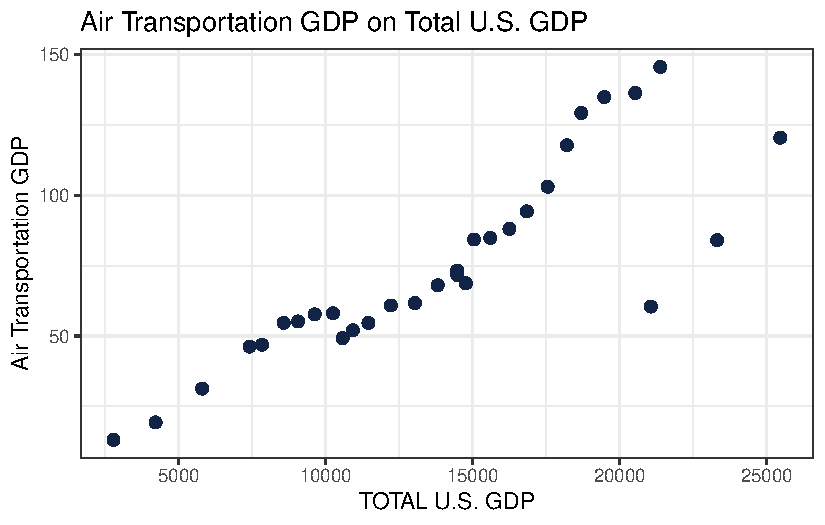
\includegraphics{Baruga_Main_files/figure-pdf/unnamed-chunk-2-1.pdf}

\begin{Shaded}
\begin{Highlighting}[]
\CommentTok{\# Remove rows where the Description column is NA}
\NormalTok{cleaned\_dataset }\OtherTok{\textless{}{-}}\NormalTok{ dataset }\SpecialCharTok{\%\textgreater{}\%} \FunctionTok{filter}\NormalTok{(}\SpecialCharTok{!}\FunctionTok{is.na}\NormalTok{(Description))}

\CommentTok{\# Convert year columns to numeric}
\NormalTok{cleaned\_dataset[, }\SpecialCharTok{{-}}\DecValTok{1}\NormalTok{] }\OtherTok{\textless{}{-}} \FunctionTok{lapply}\NormalTok{(cleaned\_dataset[, }\SpecialCharTok{{-}}\DecValTok{1}\NormalTok{], as.numeric)}

\CommentTok{\# Check if the conversion was successful}
\FunctionTok{str}\NormalTok{(cleaned\_dataset)}
\end{Highlighting}
\end{Shaded}

\begin{verbatim}
tibble [14 x 16] (S3: tbl_df/tbl/data.frame)
 $ Description: chr [1:14] "Total government revenues" "Federal" "State and local" "Total government expenditures" ...
 $ 2007       : num [1:14] 163884 53967 109917 268843 243373 ...
 $ 2008       : num [1:14] 163222 52102 111120 284343 256501 ...
 $ 2009       : num [1:14] 157684 47287 110397 300267 270478 ...
 $ 2010       : num [1:14] 160472 47244 113227 303516 271470 ...
 $ 2011       : num [1:14] 171324 50310 121014 303784 270602 ...
 $ 2012       : num [1:14] 179173 54473 124699 314024 281248 ...
 $ 2013       : num [1:14] 174527 50686 123841 309276 277065 ...
 $ 2014       : num [1:14] 183537 54161 129376 324000 291241 ...
 $ 2015       : num [1:14] 194195 56714 137481 329551 297255 ...
 $ 2016       : num [1:14] 194420 57279 137141 339439 304305 ...
 $ 2017       : num [1:14] 203528 57628 145900 355374 318231 ...
 $ 2018       : num [1:14] 213373 60035 153338 370884 337150 ...
 $ 2019       : num [1:14] 228293 62142 166150 384211 349118 ...
 $ 2020       : num [1:14] 200560 53719 146842 404177 362396 ...
 $ 2021       : num [1:14] 196163 53503 142660 398764 358148 ...
\end{verbatim}

\textbf{Descriptive Statistics}

\begin{Shaded}
\begin{Highlighting}[]
\CommentTok{\# Calculate summary statistics for numeric columns}
\NormalTok{descriptive\_stats }\OtherTok{\textless{}{-}}\NormalTok{ cleaned\_dataset }\SpecialCharTok{\%\textgreater{}\%}
  \FunctionTok{summarise}\NormalTok{(}\FunctionTok{across}\NormalTok{(}\FunctionTok{where}\NormalTok{(is.numeric), }\FunctionTok{list}\NormalTok{(}
    \AttributeTok{mean =} \SpecialCharTok{\textasciitilde{}} \FunctionTok{mean}\NormalTok{(., }\AttributeTok{na.rm =} \ConstantTok{TRUE}\NormalTok{),}
    \AttributeTok{median =} \SpecialCharTok{\textasciitilde{}} \FunctionTok{median}\NormalTok{(., }\AttributeTok{na.rm =} \ConstantTok{TRUE}\NormalTok{),}
    \AttributeTok{std\_dev =} \SpecialCharTok{\textasciitilde{}} \FunctionTok{sd}\NormalTok{(., }\AttributeTok{na.rm =} \ConstantTok{TRUE}\NormalTok{)}
\NormalTok{  )))}

\CommentTok{\# View the descriptive statistics}
\FunctionTok{print}\NormalTok{(descriptive\_stats)}
\end{Highlighting}
\end{Shaded}

\begin{verbatim}
# A tibble: 1 x 45
  `2007_mean` `2007_median` `2007_std_dev` `2008_mean` `2008_median`
        <dbl>         <dbl>          <dbl>       <dbl>         <dbl>
1     130433.       109917.         97623.     135138.       111120.
# i 40 more variables: `2008_std_dev` <dbl>, `2009_mean` <dbl>,
#   `2009_median` <dbl>, `2009_std_dev` <dbl>, `2010_mean` <dbl>,
#   `2010_median` <dbl>, `2010_std_dev` <dbl>, `2011_mean` <dbl>,
#   `2011_median` <dbl>, `2011_std_dev` <dbl>, `2012_mean` <dbl>,
#   `2012_median` <dbl>, `2012_std_dev` <dbl>, `2013_mean` <dbl>,
#   `2013_median` <dbl>, `2013_std_dev` <dbl>, `2014_mean` <dbl>,
#   `2014_median` <dbl>, `2014_std_dev` <dbl>, `2015_mean` <dbl>, ...
\end{verbatim}

\begin{Shaded}
\begin{Highlighting}[]
\CommentTok{\# Plot the distribution for one of the years, e.g., 2021}
\FunctionTok{hist}\NormalTok{(cleaned\_dataset}\SpecialCharTok{$}\StringTok{\textasciigrave{}}\AttributeTok{2021}\StringTok{\textasciigrave{}}\NormalTok{, }
     \AttributeTok{main =} \StringTok{"Distribution of Transportation{-}Related Revenues/Expenditures for 2021"}\NormalTok{, }
     \AttributeTok{xlab =} \StringTok{"Revenue/Expenditure (Millions)"}\NormalTok{, }
     \AttributeTok{breaks =} \DecValTok{20}\NormalTok{)}
\end{Highlighting}
\end{Shaded}

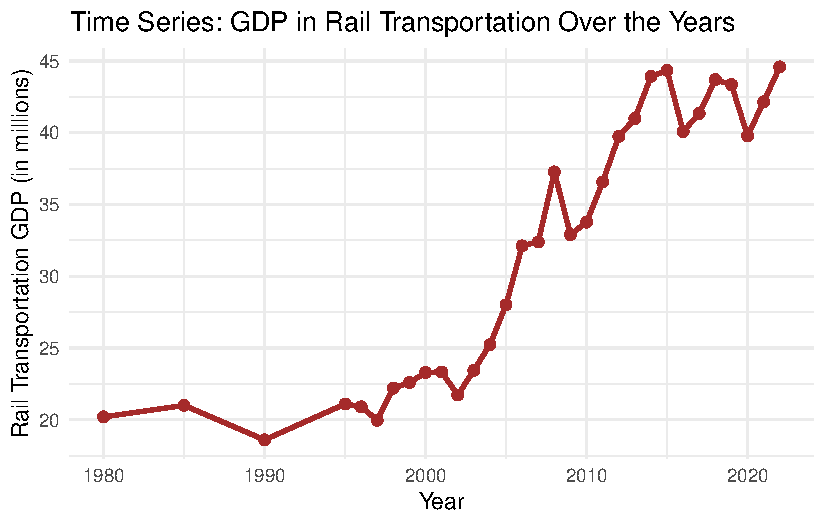
\includegraphics{Baruga_Main_files/figure-pdf/unnamed-chunk-3-1.pdf}

\begin{Shaded}
\begin{Highlighting}[]
\CommentTok{\# Example: Create a correlation matrix to identify relationships between variables}
\NormalTok{cor\_matrix }\OtherTok{\textless{}{-}} \FunctionTok{cor}\NormalTok{(cleaned\_dataset }\SpecialCharTok{\%\textgreater{}\%} \FunctionTok{select}\NormalTok{(}\FunctionTok{where}\NormalTok{(is.numeric)), }\AttributeTok{use =} \StringTok{"complete.obs"}\NormalTok{)}
\FunctionTok{print}\NormalTok{(cor\_matrix)}
\end{Highlighting}
\end{Shaded}

\begin{verbatim}
          2007      2008      2009      2010      2011      2012      2013
2007 1.0000000 0.9992200 0.9957372 0.9955944 0.9982996 0.9987699 0.9982597
2008 0.9992200 1.0000000 0.9985997 0.9984952 0.9995968 0.9998451 0.9995891
2009 0.9957372 0.9985997 1.0000000 0.9999387 0.9988945 0.9988467 0.9989537
2010 0.9955944 0.9984952 0.9999387 1.0000000 0.9990215 0.9989126 0.9990930
2011 0.9982996 0.9995968 0.9988945 0.9990215 1.0000000 0.9999100 0.9999483
2012 0.9987699 0.9998451 0.9988467 0.9989126 0.9999100 1.0000000 0.9999287
2013 0.9982597 0.9995891 0.9989537 0.9990930 0.9999483 0.9999287 1.0000000
2014 0.9985962 0.9997517 0.9988848 0.9989586 0.9999355 0.9999718 0.9999746
2015 0.9993482 0.9993916 0.9970608 0.9971437 0.9994229 0.9995078 0.9994220
2016 0.9988899 0.9997125 0.9983948 0.9984766 0.9999131 0.9999101 0.9998824
2017 0.9986660 0.9992946 0.9977322 0.9978360 0.9997184 0.9995628 0.9995986
2018 0.9989272 0.9994124 0.9977061 0.9977523 0.9995666 0.9995920 0.9996157
2019 0.9987879 0.9985028 0.9957926 0.9959504 0.9987484 0.9987679 0.9988146
2020 0.9911542 0.9955344 0.9990016 0.9991752 0.9966571 0.9963679 0.9968956
2021 0.9894631 0.9942597 0.9982861 0.9984816 0.9953152 0.9951339 0.9956841
          2014      2015      2016      2017      2018      2019      2020
2007 0.9985962 0.9993482 0.9988899 0.9986660 0.9989272 0.9987879 0.9911542
2008 0.9997517 0.9993916 0.9997125 0.9992946 0.9994124 0.9985028 0.9955344
2009 0.9988848 0.9970608 0.9983948 0.9977322 0.9977061 0.9957926 0.9990016
2010 0.9989586 0.9971437 0.9984766 0.9978360 0.9977523 0.9959504 0.9991752
2011 0.9999355 0.9994229 0.9999131 0.9997184 0.9995666 0.9987484 0.9966571
2012 0.9999718 0.9995078 0.9999101 0.9995628 0.9995920 0.9987679 0.9963679
2013 0.9999746 0.9994220 0.9998824 0.9995986 0.9996157 0.9988146 0.9968956
2014 1.0000000 0.9995464 0.9999361 0.9996537 0.9997081 0.9989196 0.9965499
2015 0.9995464 1.0000000 0.9997745 0.9997836 0.9998933 0.9997817 0.9937224
2016 0.9999361 0.9997745 1.0000000 0.9998653 0.9998327 0.9992473 0.9956970
2017 0.9996537 0.9997836 0.9998653 1.0000000 0.9998272 0.9994682 0.9948384
2018 0.9997081 0.9998933 0.9998327 0.9998272 1.0000000 0.9996941 0.9948117
2019 0.9989196 0.9997817 0.9992473 0.9994682 0.9996941 1.0000000 0.9924318
2020 0.9965499 0.9937224 0.9956970 0.9948384 0.9948117 0.9924318 1.0000000
2021 0.9952895 0.9920435 0.9942353 0.9930950 0.9932298 0.9905877 0.9998203
          2021
2007 0.9894631
2008 0.9942597
2009 0.9982861
2010 0.9984816
2011 0.9953152
2012 0.9951339
2013 0.9956841
2014 0.9952895
2015 0.9920435
2016 0.9942353
2017 0.9930950
2018 0.9932298
2019 0.9905877
2020 0.9998203
2021 1.0000000
\end{verbatim}

\begin{Shaded}
\begin{Highlighting}[]
\CommentTok{\# Visualize correlations (optional)}
\FunctionTok{library}\NormalTok{(corrplot)}
\end{Highlighting}
\end{Shaded}

\begin{verbatim}
corrplot 0.92 loaded
\end{verbatim}

\begin{Shaded}
\begin{Highlighting}[]
\FunctionTok{corrplot}\NormalTok{(cor\_matrix, }\AttributeTok{method =} \StringTok{"circle"}\NormalTok{)}
\end{Highlighting}
\end{Shaded}

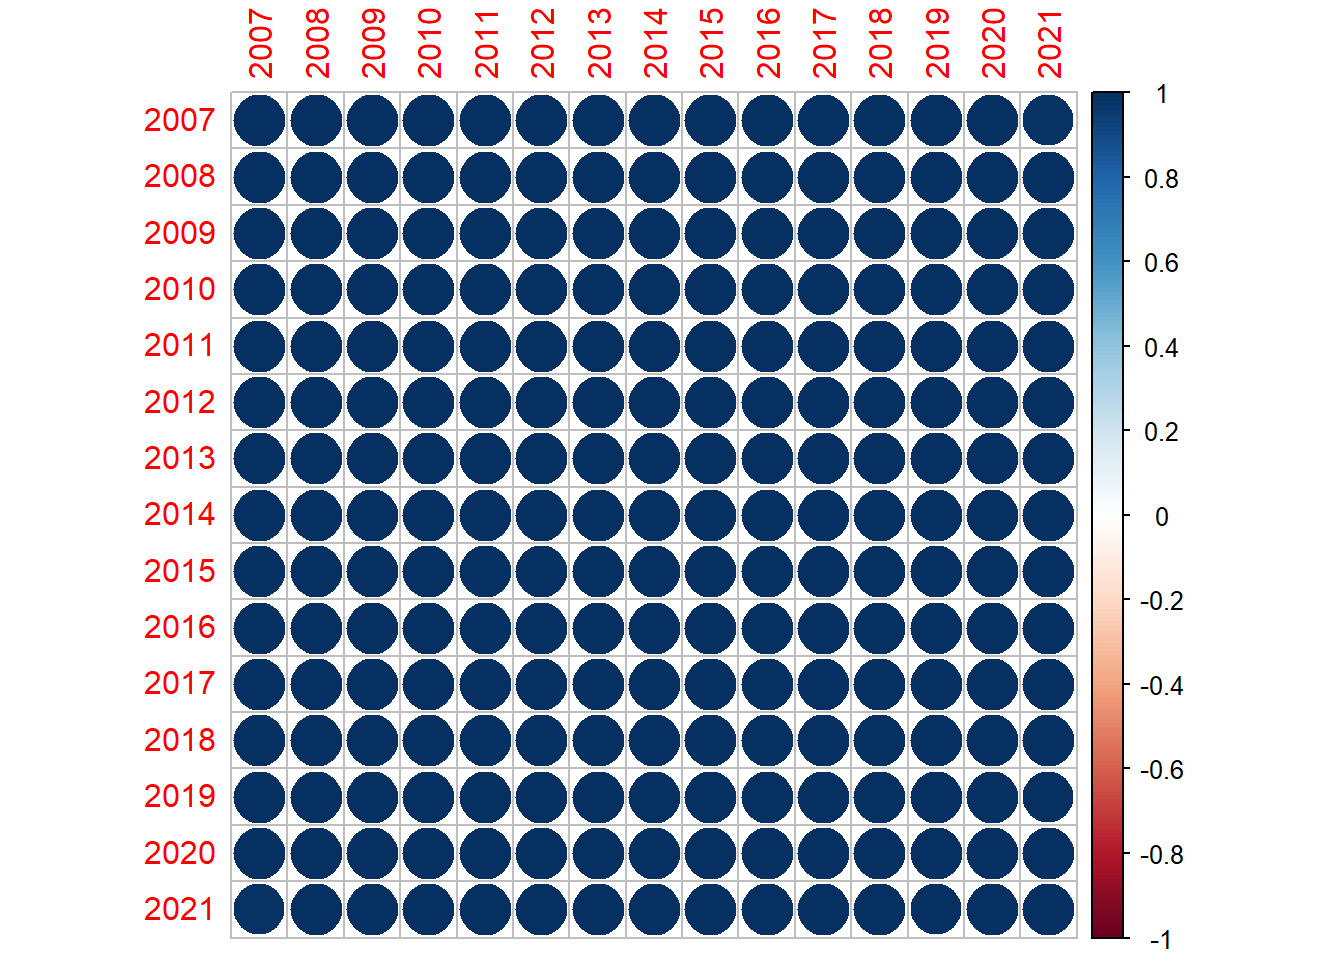
\includegraphics{Baruga_Main_files/figure-pdf/unnamed-chunk-3-2.pdf}

\section{Jupyter Notebooks}\label{jupyter-notebooks-2}

\subsection{Week 4}\label{week-4-2}

\textbf{Markdown title}

Markdown Lists:

\begin{itemize}
\tightlist
\item
  Item 1
\item
  Item 2
\item
  Item 3
\end{itemize}

Enumarated list

\begin{enumerate}
\def\labelenumi{\arabic{enumi}.}
\tightlist
\item
  Hola
\item
  Hi
\item
  Namaste
\end{enumerate}

We can do \textbf{bold}, or \emph{italic}

\begin{Shaded}
\begin{Highlighting}[]
\CommentTok{\# Importing Numpy with nickname np}
\ImportTok{import}\NormalTok{ numpy }\ImportTok{as}\NormalTok{ np}
\NormalTok{np.absolute(}\OperatorTok{{-}}\DecValTok{1}\NormalTok{)}
\NormalTok{arr }\OperatorTok{=}\NormalTok{ np.array([}\DecValTok{1}\NormalTok{, }\DecValTok{2}\NormalTok{, }\DecValTok{3}\NormalTok{, }\DecValTok{4}\NormalTok{, }\DecValTok{5}\NormalTok{])}
\BuiltInTok{print}\NormalTok{(arr)}
\end{Highlighting}
\end{Shaded}

\begin{verbatim}
[1 2 3 4 5]
\end{verbatim}

\begin{Shaded}
\begin{Highlighting}[]
\CommentTok{\# Lists are native to python}
\NormalTok{my\_list }\OperatorTok{=}\NormalTok{ [}\DecValTok{1}\NormalTok{, }\DecValTok{2}\NormalTok{, }\DecValTok{3}\NormalTok{, }\DecValTok{4}\NormalTok{, }\DecValTok{5}\NormalTok{]}
\BuiltInTok{print}\NormalTok{(my\_list)}
\end{Highlighting}
\end{Shaded}

\begin{verbatim}
[1, 2, 3, 4, 5]
\end{verbatim}

\begin{Shaded}
\begin{Highlighting}[]
\CommentTok{\# Dataframes, so we need pandas library}
\ImportTok{import}\NormalTok{ pandas }\ImportTok{as}\NormalTok{ pd}
\NormalTok{data }\OperatorTok{=}\NormalTok{ \{}\StringTok{\textquotesingle{}Ozone\textquotesingle{}}\NormalTok{: [}\DecValTok{41}\NormalTok{, }\DecValTok{36}\NormalTok{, }\DecValTok{12}\NormalTok{], }\StringTok{\textquotesingle{}Temp\textquotesingle{}}\NormalTok{: [}\DecValTok{67}\NormalTok{, }\DecValTok{72}\NormalTok{, }\DecValTok{74}\NormalTok{]\}}
\NormalTok{df }\OperatorTok{=}\NormalTok{ pd.DataFrame(data)}
\BuiltInTok{print}\NormalTok{(df)}
\end{Highlighting}
\end{Shaded}

\begin{verbatim}
   Ozone  Temp
0     41    67
1     36    72
2     12    74
\end{verbatim}

\textbf{4. Loading csv files}

To load .csv files into a `DataFrame', we use pandas function read\_csv

\begin{Shaded}
\begin{Highlighting}[]
\NormalTok{df }\OperatorTok{=}\NormalTok{ pd.read\_csv(}\StringTok{\textquotesingle{}/Users/derrickmarkbavaudbaruga/Documents/fall 2024/CSC 477/Week 2/airquality\_datasets.csv\textquotesingle{}}\NormalTok{)}
\CommentTok{\# Summary of the dataset}
\BuiltInTok{print}\NormalTok{(df.info())}
\BuiltInTok{print}\NormalTok{(df.describe())}
\end{Highlighting}
\end{Shaded}

\begin{verbatim}
<class 'pandas.core.frame.DataFrame'>
RangeIndex: 153 entries, 0 to 152
Data columns (total 6 columns):
 #   Column   Non-Null Count  Dtype  
---  ------   --------------  -----  
 0   Ozone    116 non-null    float64
 1   Solar.R  146 non-null    float64
 2   Wind     153 non-null    float64
 3   Temp     153 non-null    int64  
 4   Month    153 non-null    int64  
 5   Day      153 non-null    int64  
dtypes: float64(3), int64(3)
memory usage: 7.3 KB
None
            Ozone     Solar.R        Wind        Temp       Month         Day
count  116.000000  146.000000  153.000000  153.000000  153.000000  153.000000
mean    42.129310  185.931507    9.957516   77.882353    6.993464   15.803922
std     32.987885   90.058422    3.523001    9.465270    1.416522    8.864520
min      1.000000    7.000000    1.700000   56.000000    5.000000    1.000000
25%     18.000000  115.750000    7.400000   72.000000    6.000000    8.000000
50%     31.500000  205.000000    9.700000   79.000000    7.000000   16.000000
75%     63.250000  258.750000   11.500000   85.000000    8.000000   23.000000
max    168.000000  334.000000   20.700000   97.000000    9.000000   31.000000
\end{verbatim}

\begin{Shaded}
\begin{Highlighting}[]
\ImportTok{import}\NormalTok{ matplotlib.pyplot }\ImportTok{as}\NormalTok{ plt}

\CommentTok{\# Ozone Histogram}
\NormalTok{plt.figure(figsize}\OperatorTok{=}\NormalTok{(}\DecValTok{8}\NormalTok{, }\DecValTok{6}\NormalTok{))}
\NormalTok{plt.hist(df[}\StringTok{\textquotesingle{}Ozone\textquotesingle{}}\NormalTok{].dropna(), bins}\OperatorTok{=}\DecValTok{20}\NormalTok{, color}\OperatorTok{=}\StringTok{\textquotesingle{}blue\textquotesingle{}}\NormalTok{, edgecolor}\OperatorTok{=}\StringTok{\textquotesingle{}black\textquotesingle{}}\NormalTok{)}
\NormalTok{plt.title(}\StringTok{\textquotesingle{}Distribution of Ozone Levels\textquotesingle{}}\NormalTok{)}
\NormalTok{plt.xlabel(}\StringTok{\textquotesingle{}Ozone (ppb)\textquotesingle{}}\NormalTok{)}
\NormalTok{plt.ylabel(}\StringTok{\textquotesingle{}Frequency\textquotesingle{}}\NormalTok{)}
\NormalTok{plt.show()}
\end{Highlighting}
\end{Shaded}

\begin{figure}[H]

{\centering 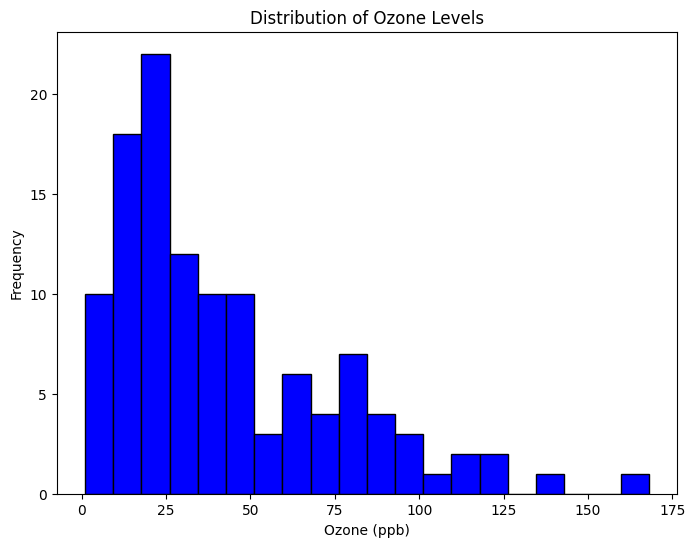
\includegraphics{week4_baruga_python_files/week4_baruga_python_6_0.png}

}

\caption{png}

\end{figure}%

\begin{Shaded}
\begin{Highlighting}[]
\CommentTok{\# Temp Histogram}
\NormalTok{plt.figure(figsize}\OperatorTok{=}\NormalTok{(}\DecValTok{8}\NormalTok{, }\DecValTok{6}\NormalTok{))}
\NormalTok{plt.hist(df[}\StringTok{\textquotesingle{}Temp\textquotesingle{}}\NormalTok{].dropna(), bins}\OperatorTok{=}\DecValTok{20}\NormalTok{, color}\OperatorTok{=}\StringTok{\textquotesingle{}orange\textquotesingle{}}\NormalTok{, edgecolor}\OperatorTok{=}\StringTok{\textquotesingle{}black\textquotesingle{}}\NormalTok{)}
\NormalTok{plt.title(}\StringTok{\textquotesingle{}Distribution of Temperature\textquotesingle{}}\NormalTok{)}
\NormalTok{plt.xlabel(}\StringTok{\textquotesingle{}Temperature (°F)\textquotesingle{}}\NormalTok{)}
\NormalTok{plt.ylabel(}\StringTok{\textquotesingle{}Frequency\textquotesingle{}}\NormalTok{)}
\NormalTok{plt.show()}
\end{Highlighting}
\end{Shaded}

\begin{figure}[H]

{\centering 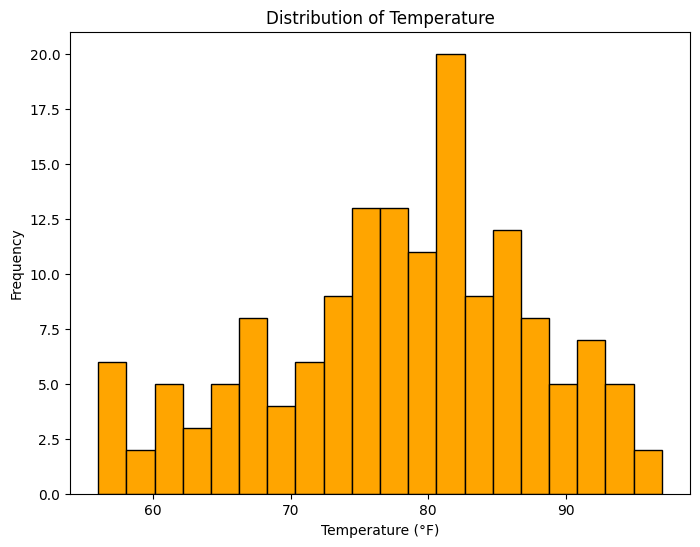
\includegraphics{week4_baruga_python_files/week4_baruga_python_7_0.png}

}

\caption{png}

\end{figure}%

\begin{Shaded}
\begin{Highlighting}[]
\CommentTok{\# Boxplot for Ozone}
\NormalTok{plt.figure(figsize}\OperatorTok{=}\NormalTok{(}\DecValTok{8}\NormalTok{, }\DecValTok{6}\NormalTok{))}
\NormalTok{plt.boxplot(df[}\StringTok{\textquotesingle{}Ozone\textquotesingle{}}\NormalTok{].dropna())}
\NormalTok{plt.title(}\StringTok{\textquotesingle{}Boxplot of Ozone Levels\textquotesingle{}}\NormalTok{)}
\NormalTok{plt.ylabel(}\StringTok{\textquotesingle{}Ozone (ppb)\textquotesingle{}}\NormalTok{)}
\NormalTok{plt.show()}
\end{Highlighting}
\end{Shaded}

\begin{figure}[H]

{\centering 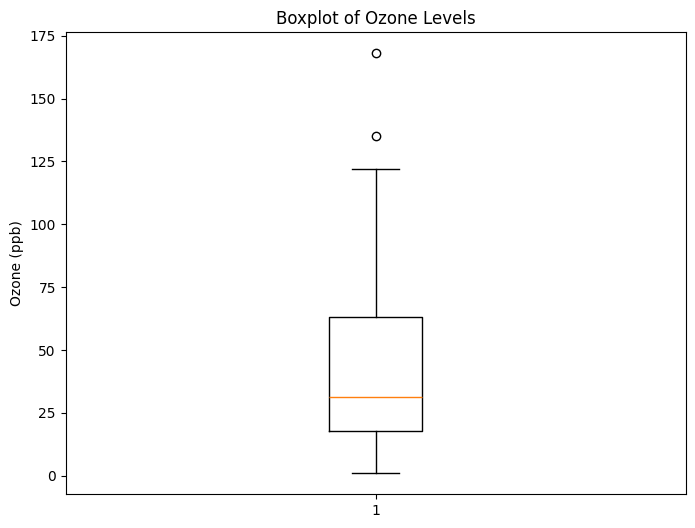
\includegraphics{week4_baruga_python_files/week4_baruga_python_8_0.png}

}

\caption{png}

\end{figure}%

\begin{Shaded}
\begin{Highlighting}[]
\CommentTok{\# Boxplot for Temp}
\NormalTok{plt.figure(figsize}\OperatorTok{=}\NormalTok{(}\DecValTok{8}\NormalTok{, }\DecValTok{6}\NormalTok{))}
\NormalTok{plt.boxplot(df[}\StringTok{\textquotesingle{}Temp\textquotesingle{}}\NormalTok{].dropna())}
\NormalTok{plt.title(}\StringTok{\textquotesingle{}Boxplot of Temperature\textquotesingle{}}\NormalTok{)}
\NormalTok{plt.ylabel(}\StringTok{\textquotesingle{}Temperature (°F)\textquotesingle{}}\NormalTok{)}
\NormalTok{plt.show()}
\end{Highlighting}
\end{Shaded}

\begin{figure}[H]

{\centering 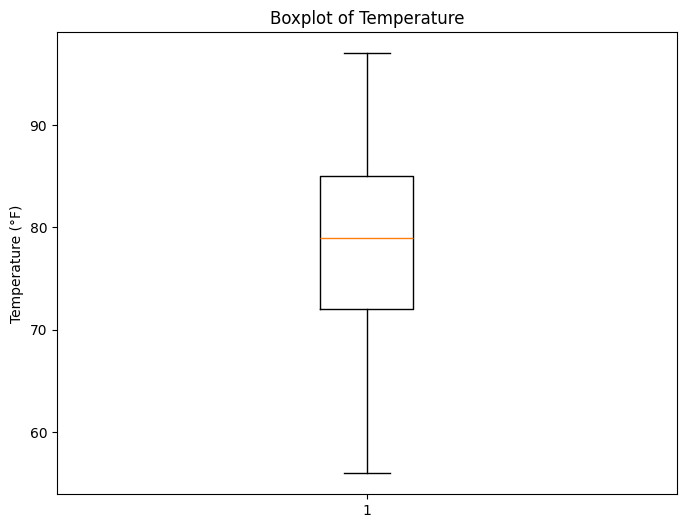
\includegraphics{week4_baruga_python_files/week4_baruga_python_9_0.png}

}

\caption{png}

\end{figure}%

\subsection{Week 5}\label{week-5-2}

\textbf{1. Introduction to Plotnine}

plotnine is a data visualization package for Python based on the Grammar
of Graphics, which is a system for understanding and building plots. The
grammar describes how plots are constructed by combining data, aesthetic
mappings, geometric objects, and other components.

To begin, you'll need to install the plotnine package if you don't have
it installed:

\begin{Shaded}
\begin{Highlighting}[]
\CommentTok{\# !pip install plotnine}
\end{Highlighting}
\end{Shaded}

\textbf{2. The Grammar of Graphics}

The Grammar of Graphics consists of the following key components:

\begin{itemize}
\tightlist
\item
  Data: The data you want to visualize.
\item
  Aesthetics (aes): How the data is mapped to visual properties, such as
  x and y coordinates, color, size, etc.
\item
  Geometries (geom): The type of plot, like points, lines, bars, etc.
\item
  Facets: Subplots based on the data.
\item
  Scales: Control the mapping from data to aesthetic properties.
\item
  Coordinate systems: Adjust how data is projected on the plane
  (Cartesian, rotations, polar, etc.).
\item
  Themes: Adjust the non-data elements like background, labels,
  gridlines, etc.
\end{itemize}

\textbf{3. Creating Your First Plot} Let's begin by creating a simple
scatter plot using the famous mtcars dataset. We'll show how to set up
the basic structure and gradually build complexity.

\begin{Shaded}
\begin{Highlighting}[]
\CommentTok{\# Import required libraries}
\ImportTok{import}\NormalTok{ pandas }\ImportTok{as}\NormalTok{ pd}
\ImportTok{from}\NormalTok{ plotnine }\ImportTok{import}\NormalTok{ ggplot, aes, geom\_point, labs}

\CommentTok{\# Load the mtcars dataset}
\NormalTok{mtcars }\OperatorTok{=}\NormalTok{ pd.read\_csv(}\StringTok{\textquotesingle{}https://raw.githubusercontent.com/selva86/datasets/master/mtcars.csv\textquotesingle{}}\NormalTok{)}

\CommentTok{\# Create a basic scatter plot}
\NormalTok{(ggplot(mtcars, aes(x}\OperatorTok{=}\StringTok{\textquotesingle{}wt\textquotesingle{}}\NormalTok{, y}\OperatorTok{=}\StringTok{\textquotesingle{}mpg\textquotesingle{}}\NormalTok{)) }\OperatorTok{+}
\NormalTok{ geom\_point() }\OperatorTok{+}
\NormalTok{ labs(title}\OperatorTok{=}\StringTok{\textquotesingle{}Scatter Plot of MPG vs Weight\textquotesingle{}}\NormalTok{,}
\NormalTok{      x}\OperatorTok{=}\StringTok{\textquotesingle{}Weight (1000 lbs)\textquotesingle{}}\NormalTok{,}
\NormalTok{      y}\OperatorTok{=}\StringTok{\textquotesingle{}Miles per Gallon\textquotesingle{}}\NormalTok{))}
\end{Highlighting}
\end{Shaded}

\begin{verbatim}
<string>:3: FutureWarning: Using repr(plot) to draw and show the plot figure is deprecated and will be removed in a future version. Use plot.show().
<Figure Size: (640 x 480)>
\end{verbatim}

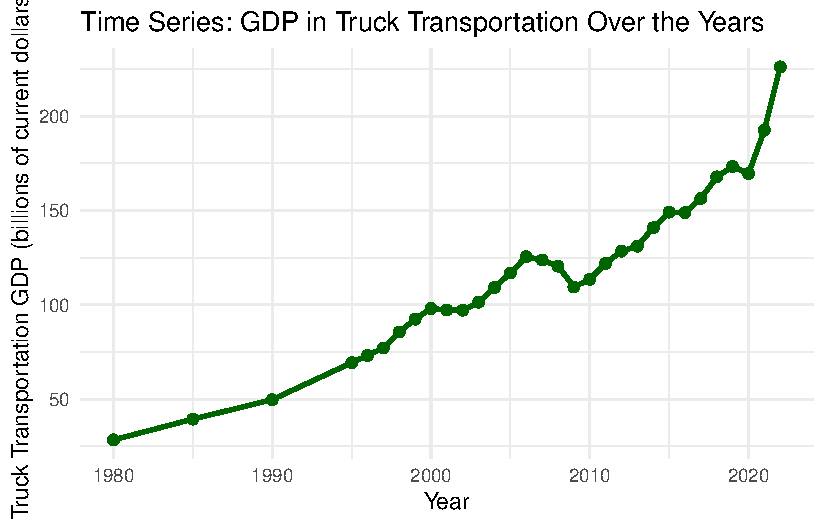
\includegraphics{Baruga_Main_files/figure-pdf/unnamed-chunk-5-1.pdf}

** 4. Adding Aesthetic Mappings**

In the Grammar of Graphics, aesthetics control how data points are
represented visually. You can map variables to size, color, shape, and
more.

Example: Color by cyl (number of cylinders)

\begin{Shaded}
\begin{Highlighting}[]
\NormalTok{(ggplot(mtcars, aes(x}\OperatorTok{=}\StringTok{\textquotesingle{}wt\textquotesingle{}}\NormalTok{, y}\OperatorTok{=}\StringTok{\textquotesingle{}mpg\textquotesingle{}}\NormalTok{, color}\OperatorTok{=}\StringTok{\textquotesingle{}factor(cyl)\textquotesingle{}}\NormalTok{)) }\OperatorTok{+}
\NormalTok{ geom\_point() }\OperatorTok{+}
\NormalTok{ labs(title}\OperatorTok{=}\StringTok{\textquotesingle{}MPG vs Weight by Cylinder\textquotesingle{}}\NormalTok{,}
\NormalTok{      x}\OperatorTok{=}\StringTok{\textquotesingle{}Weight (1000 lbs)\textquotesingle{}}\NormalTok{,}
\NormalTok{      y}\OperatorTok{=}\StringTok{\textquotesingle{}Miles per Gallon\textquotesingle{}}\NormalTok{,}
\NormalTok{      color}\OperatorTok{=}\StringTok{\textquotesingle{}Cylinders\textquotesingle{}}\NormalTok{))}
\end{Highlighting}
\end{Shaded}

\begin{verbatim}
<string>:1: FutureWarning: Using repr(plot) to draw and show the plot figure is deprecated and will be removed in a future version. Use plot.show().
<Figure Size: (640 x 480)>
\end{verbatim}

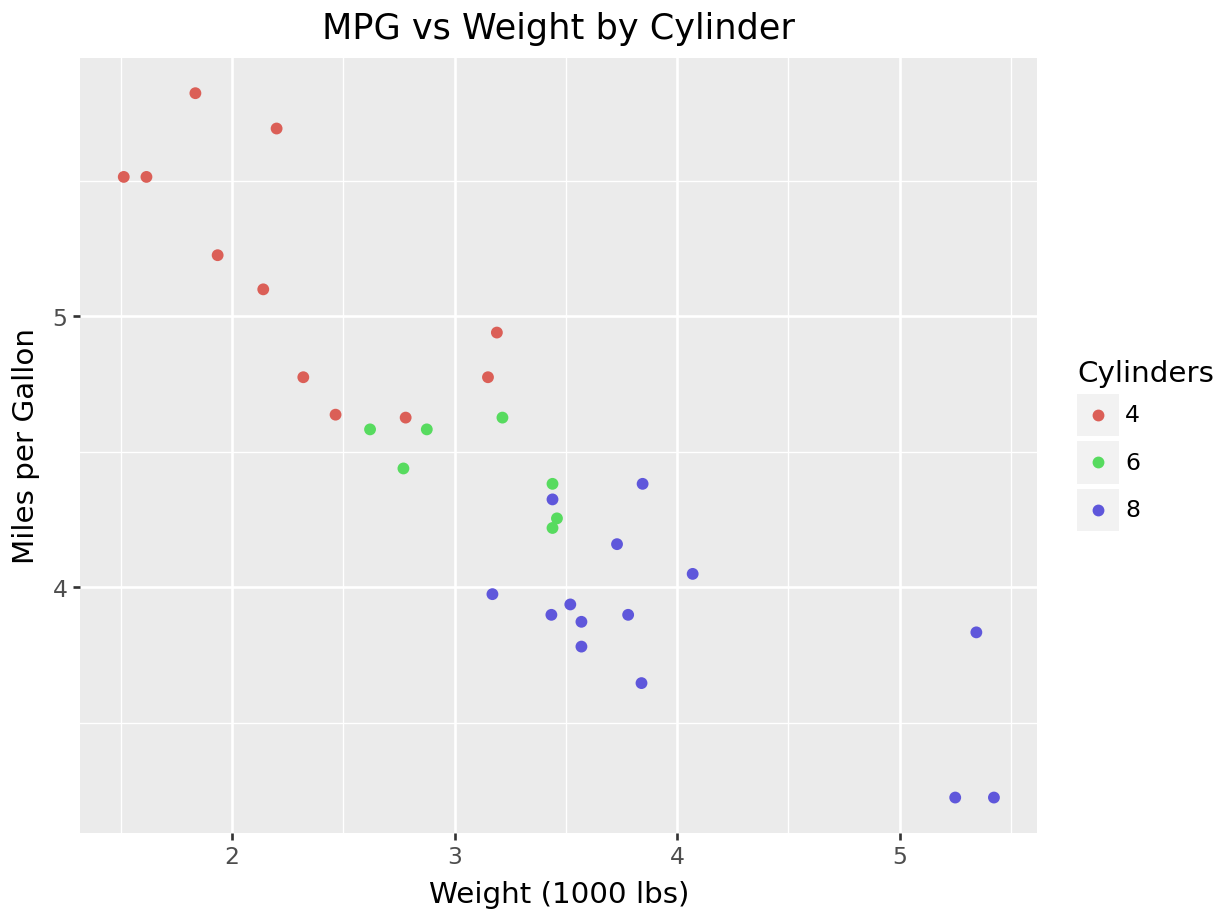
\includegraphics{Baruga_Main_files/figure-pdf/unnamed-chunk-6-3.pdf}

Example: Size by horsepower (hp)

\begin{Shaded}
\begin{Highlighting}[]
\NormalTok{(ggplot(mtcars, aes(x}\OperatorTok{=}\StringTok{\textquotesingle{}wt\textquotesingle{}}\NormalTok{, y}\OperatorTok{=}\StringTok{\textquotesingle{}mpg\textquotesingle{}}\NormalTok{, color}\OperatorTok{=}\StringTok{\textquotesingle{}factor(cyl)\textquotesingle{}}\NormalTok{, size}\OperatorTok{=}\StringTok{\textquotesingle{}hp\textquotesingle{}}\NormalTok{)) }\OperatorTok{+}
\NormalTok{ geom\_point() }\OperatorTok{+}
\NormalTok{ labs(title}\OperatorTok{=}\StringTok{\textquotesingle{}MPG vs Weight by Cylinder and Horsepower\textquotesingle{}}\NormalTok{,}
\NormalTok{      x}\OperatorTok{=}\StringTok{\textquotesingle{}Weight (1000 lbs)\textquotesingle{}}\NormalTok{,}
\NormalTok{      y}\OperatorTok{=}\StringTok{\textquotesingle{}Miles per Gallon\textquotesingle{}}\NormalTok{,}
\NormalTok{      color}\OperatorTok{=}\StringTok{\textquotesingle{}Cylinders\textquotesingle{}}\NormalTok{,}
\NormalTok{      size}\OperatorTok{=}\StringTok{\textquotesingle{}Horsepower\textquotesingle{}}\NormalTok{))}
\end{Highlighting}
\end{Shaded}

\begin{verbatim}
<string>:1: FutureWarning: Using repr(plot) to draw and show the plot figure is deprecated and will be removed in a future version. Use plot.show().
<Figure Size: (640 x 480)>
\end{verbatim}

\includegraphics{Baruga_Main_files/figure-pdf/unnamed-chunk-7-5.pdf}

\textbf{5. Geometric Objects}

geom\_* specifies the type of plot. You can create scatter plots, line
charts, bar plots, histograms, etc.

Example: Adding a smooth line (geom\_smooth)

\begin{Shaded}
\begin{Highlighting}[]
\ImportTok{from}\NormalTok{ plotnine }\ImportTok{import}\NormalTok{ geom\_smooth}

\NormalTok{(ggplot(mtcars, aes(x}\OperatorTok{=}\StringTok{\textquotesingle{}wt\textquotesingle{}}\NormalTok{, y}\OperatorTok{=}\StringTok{\textquotesingle{}mpg\textquotesingle{}}\NormalTok{)) }\OperatorTok{+}
\NormalTok{ geom\_point() }\OperatorTok{+}
\NormalTok{ geom\_smooth(method}\OperatorTok{=}\StringTok{\textquotesingle{}lm\textquotesingle{}}\NormalTok{) }\OperatorTok{+}  \CommentTok{\# Linear regression line}
\NormalTok{ labs(title}\OperatorTok{=}\StringTok{\textquotesingle{}MPG vs Weight with Regression Line\textquotesingle{}}\NormalTok{,}
\NormalTok{      x}\OperatorTok{=}\StringTok{\textquotesingle{}Weight (1000 lbs)\textquotesingle{}}\NormalTok{,}
\NormalTok{      y}\OperatorTok{=}\StringTok{\textquotesingle{}Miles per Gallon\textquotesingle{}}\NormalTok{))}
\end{Highlighting}
\end{Shaded}

\begin{verbatim}
<string>:2: FutureWarning: Using repr(plot) to draw and show the plot figure is deprecated and will be removed in a future version. Use plot.show().
<Figure Size: (640 x 480)>
\end{verbatim}

\includegraphics{Baruga_Main_files/figure-pdf/unnamed-chunk-8-7.pdf}

\textbf{6. Faceting}

Faceting allows you to split your plot into multiple panels based on a
factor.

Example: Facet by cyl

\begin{Shaded}
\begin{Highlighting}[]
\ImportTok{from}\NormalTok{ plotnine }\ImportTok{import}\NormalTok{ facet\_wrap}

\NormalTok{(ggplot(mtcars, aes(x}\OperatorTok{=}\StringTok{\textquotesingle{}wt\textquotesingle{}}\NormalTok{, y}\OperatorTok{=}\StringTok{\textquotesingle{}mpg\textquotesingle{}}\NormalTok{)) }\OperatorTok{+}
\NormalTok{ geom\_point() }\OperatorTok{+}
\NormalTok{ facet\_wrap(}\StringTok{\textquotesingle{}\textasciitilde{}cyl\textquotesingle{}}\NormalTok{) }\OperatorTok{+}  \CommentTok{\# Split into subplots by cylinders}
\NormalTok{ labs(title}\OperatorTok{=}\StringTok{\textquotesingle{}MPG vs Weight Faceted by Cylinder\textquotesingle{}}\NormalTok{,}
\NormalTok{      x}\OperatorTok{=}\StringTok{\textquotesingle{}Weight (1000 lbs)\textquotesingle{}}\NormalTok{,}
\NormalTok{      y}\OperatorTok{=}\StringTok{\textquotesingle{}Miles per Gallon\textquotesingle{}}\NormalTok{))}
\end{Highlighting}
\end{Shaded}

\begin{verbatim}
<string>:2: FutureWarning: Using repr(plot) to draw and show the plot figure is deprecated and will be removed in a future version. Use plot.show().
<Figure Size: (640 x 480)>
\end{verbatim}

\includegraphics{Baruga_Main_files/figure-pdf/unnamed-chunk-9-9.pdf}

\textbf{7. Customizing Scales}

Scales control the mapping from data to aesthetic attributes. You can
customize scales for color, size, and more.

Example: Custom Color Scale

\begin{Shaded}
\begin{Highlighting}[]
\ImportTok{from}\NormalTok{ plotnine }\ImportTok{import}\NormalTok{ scale\_color\_manual}

\NormalTok{(ggplot(mtcars, aes(x}\OperatorTok{=}\StringTok{\textquotesingle{}wt\textquotesingle{}}\NormalTok{, y}\OperatorTok{=}\StringTok{\textquotesingle{}mpg\textquotesingle{}}\NormalTok{, color}\OperatorTok{=}\StringTok{\textquotesingle{}factor(cyl)\textquotesingle{}}\NormalTok{)) }\OperatorTok{+}
\NormalTok{ geom\_point() }\OperatorTok{+}
\NormalTok{ scale\_color\_manual(values}\OperatorTok{=}\NormalTok{[}\StringTok{\textquotesingle{}\#1f77b4\textquotesingle{}}\NormalTok{, }\StringTok{\textquotesingle{}\#ff7f0e\textquotesingle{}}\NormalTok{, }\StringTok{\textquotesingle{}\#2ca02c\textquotesingle{}}\NormalTok{]) }\OperatorTok{+}  \CommentTok{\# Custom colors}
\NormalTok{ labs(title}\OperatorTok{=}\StringTok{\textquotesingle{}MPG vs Weight with Custom Colors\textquotesingle{}}\NormalTok{,}
\NormalTok{      x}\OperatorTok{=}\StringTok{\textquotesingle{}Weight (1000 lbs)\textquotesingle{}}\NormalTok{,}
\NormalTok{      y}\OperatorTok{=}\StringTok{\textquotesingle{}Miles per Gallon\textquotesingle{}}\NormalTok{,}
\NormalTok{      color}\OperatorTok{=}\StringTok{\textquotesingle{}Cylinders\textquotesingle{}}\NormalTok{))}
\end{Highlighting}
\end{Shaded}

\begin{verbatim}
<string>:2: FutureWarning: Using repr(plot) to draw and show the plot figure is deprecated and will be removed in a future version. Use plot.show().
<Figure Size: (640 x 480)>
\end{verbatim}

\includegraphics{Baruga_Main_files/figure-pdf/unnamed-chunk-10-11.pdf}

\textbf{8. Flip Coordinates} Create a bar plot showing distribution of
cylinders

Example: Fliping coordinates axis

\begin{Shaded}
\begin{Highlighting}[]
\ImportTok{import}\NormalTok{ pandas }\ImportTok{as}\NormalTok{ pd}

\ImportTok{from}\NormalTok{ plotnine }\ImportTok{import}\NormalTok{ ggplot, aes, geom\_bar, coord\_flip, labs}

\CommentTok{\# Load the mtcars dataset}
\NormalTok{mtcars }\OperatorTok{=}\NormalTok{ pd.read\_csv(}\StringTok{\textquotesingle{}https://raw.githubusercontent.com/selva86/datasets/master/mtcars.csv\textquotesingle{}}\NormalTok{)}

\CommentTok{\# Create a bar plot showing distribution of cylinders}
\NormalTok{(ggplot(mtcars, aes(x}\OperatorTok{=}\StringTok{\textquotesingle{}factor(cyl)\textquotesingle{}}\NormalTok{, fill}\OperatorTok{=}\StringTok{\textquotesingle{}factor(cyl)\textquotesingle{}}\NormalTok{)) }\OperatorTok{+}
\NormalTok{ geom\_bar(width}\OperatorTok{=}\DecValTok{1}\NormalTok{) }\OperatorTok{+}
\NormalTok{ coord\_flip() }\OperatorTok{+}  \CommentTok{\# Flip coordinates as a simple workaround}
\NormalTok{ labs(title}\OperatorTok{=}\StringTok{\textquotesingle{}Distribution of Cylinders\textquotesingle{}}\NormalTok{,}
\NormalTok{      x}\OperatorTok{=}\StringTok{\textquotesingle{}Cylinders\textquotesingle{}}\NormalTok{,}
\NormalTok{      fill}\OperatorTok{=}\StringTok{\textquotesingle{}Cylinders\textquotesingle{}}\NormalTok{))}
\end{Highlighting}
\end{Shaded}

\begin{verbatim}
<string>:3: FutureWarning: Using repr(plot) to draw and show the plot figure is deprecated and will be removed in a future version. Use plot.show().
<Figure Size: (640 x 480)>
\end{verbatim}

\includegraphics{Baruga_Main_files/figure-pdf/unnamed-chunk-11-13.pdf}

\textbf{9. Themes}

Themes allow you to adjust the non-data aspects of the plot, such as
background, axis labels, and gridlines.

Example: Apply a Minimal Theme

\begin{Shaded}
\begin{Highlighting}[]
\ImportTok{from}\NormalTok{ plotnine }\ImportTok{import}\NormalTok{ theme\_minimal}

\NormalTok{(ggplot(mtcars, aes(x}\OperatorTok{=}\StringTok{\textquotesingle{}wt\textquotesingle{}}\NormalTok{, y}\OperatorTok{=}\StringTok{\textquotesingle{}mpg\textquotesingle{}}\NormalTok{)) }\OperatorTok{+}
\NormalTok{ geom\_point() }\OperatorTok{+}
\NormalTok{ theme\_minimal() }\OperatorTok{+}  \CommentTok{\# Minimalistic theme}
\NormalTok{ labs(title}\OperatorTok{=}\StringTok{\textquotesingle{}MPG vs Weight with Minimal Theme\textquotesingle{}}\NormalTok{,}
\NormalTok{      x}\OperatorTok{=}\StringTok{\textquotesingle{}Weight (1000 lbs)\textquotesingle{}}\NormalTok{,}
\NormalTok{      y}\OperatorTok{=}\StringTok{\textquotesingle{}Miles per Gallon\textquotesingle{}}\NormalTok{))}
\end{Highlighting}
\end{Shaded}

\begin{verbatim}
<string>:2: FutureWarning: Using repr(plot) to draw and show the plot figure is deprecated and will be removed in a future version. Use plot.show().
<Figure Size: (640 x 480)>
\end{verbatim}

\includegraphics{Baruga_Main_files/figure-pdf/unnamed-chunk-12-15.pdf}

\textbf{10. Saving the Plot}

You can save your plot using the save method.

Example: Save the plot

\begin{Shaded}
\begin{Highlighting}[]
\CommentTok{\# Save the plot to a file}
\NormalTok{p }\OperatorTok{=}\NormalTok{ (ggplot(mtcars, aes(x}\OperatorTok{=}\StringTok{\textquotesingle{}wt\textquotesingle{}}\NormalTok{, y}\OperatorTok{=}\StringTok{\textquotesingle{}mpg\textquotesingle{}}\NormalTok{)) }\OperatorTok{+}
\NormalTok{     geom\_point() }\OperatorTok{+}
\NormalTok{     labs(title}\OperatorTok{=}\StringTok{\textquotesingle{}MPG vs Weight\textquotesingle{}}\NormalTok{,}
\NormalTok{          x}\OperatorTok{=}\StringTok{\textquotesingle{}Weight (1000 lbs)\textquotesingle{}}\NormalTok{,}
\NormalTok{          y}\OperatorTok{=}\StringTok{\textquotesingle{}Miles per Gallon\textquotesingle{}}\NormalTok{))}

\NormalTok{p.save(}\StringTok{"mpg\_vs\_weight.png"}\NormalTok{)}
\end{Highlighting}
\end{Shaded}

\begin{verbatim}
C:\Users\toluf\AppData\Roaming\Python\Python312\site-packages\plotnine\ggplot.py:606: PlotnineWarning: Saving 6.4 x 4.8 in image.
C:\Users\toluf\AppData\Roaming\Python\Python312\site-packages\plotnine\ggplot.py:607: PlotnineWarning: Filename: mpg_vs_weight.png
\end{verbatim}

\textbf{Week 5 Midterm Report}

\textbf{Data Analysis}

\textbf{Load libraries}

\begin{Shaded}
\begin{Highlighting}[]
\ImportTok{import}\NormalTok{ torch }\ImportTok{as}\NormalTok{ tch}
\ImportTok{import}\NormalTok{ pandas }\ImportTok{as}\NormalTok{ pd}
\ImportTok{import}\NormalTok{ scipy }\ImportTok{as}\NormalTok{ sci}
\ImportTok{import}\NormalTok{ openpyxl }\ImportTok{as}\NormalTok{ opxl}
\ImportTok{import}\NormalTok{ seaborn }\ImportTok{as}\NormalTok{ sns}
\end{Highlighting}
\end{Shaded}

\textbf{Load CSV}

\begin{Shaded}
\begin{Highlighting}[]
\NormalTok{df }\OperatorTok{=}\NormalTok{ pd.read\_csv(}\StringTok{\textquotesingle{}data.csv\textquotesingle{}}\NormalTok{, low\_memory}\OperatorTok{=}\VariableTok{False}\NormalTok{)}
\end{Highlighting}
\end{Shaded}

\textbf{Summary Stats}

\begin{Shaded}
\begin{Highlighting}[]
\NormalTok{df.head()}
\end{Highlighting}
\end{Shaded}

SCRMCTRL

PPCSWGT

SEQNUM

SEX

AGE

INTTYPE

NONINT

HISP

MODE

PSSTRATA

\ldots{}

V352A

V352B

V352C

V352D

V352E

V352F

CHECK\_ITEM\_J

CHECK\_ITEM\_K

CHECK\_ITEM\_L

V353

0

2.030020e+18

4150.904836

1.0

\begin{enumerate}
\def\labelenumi{(\arabic{enumi})}
\tightlist
\item
  Male

  \begin{enumerate}
  \def\labelenumii{(\arabic{enumii})}
  \setcounter{enumii}{3}
  \tightlist
  \item
    45-64

    \begin{enumerate}
    \def\labelenumiii{(\arabic{enumiii})}
    \setcounter{enumiii}{1}
    \tightlist
    \item
      PPCS Interview - Telephone

      NaN

      \begin{enumerate}
      \def\labelenumiv{(\arabic{enumiv})}
      \tightlist
      \item
        White Only

        \begin{enumerate}
        \def\labelenumv{(\arabic{enumv})}
        \tightlist
        \item
          Computer-assisted personal interviewing

          54

          \ldots{}

          NaN

          NaN

          NaN

          NaN

          NaN

          NaN

          NaN

          NaN

          NaN

          NaN

          1

          2.030030e+18

          1601.829088

          2.0

          \begin{enumerate}
          \def\labelenumvi{(\arabic{enumvi})}
          \tightlist
          \item
            Female

            \begin{enumerate}
            \def\labelenumvii{(\arabic{enumvii})}
            \tightlist
            \item
              25-44

              \begin{enumerate}
              \def\labelenumviii{(\arabic{enumviii})}
              \tightlist
              \item
                PPCS Interview - Telephone

                NaN

                \begin{enumerate}
                \def\labelenumix{(\arabic{enumix})}
                \tightlist
                \item
                  White Only

                  \begin{enumerate}
                  \def\labelenumx{(\arabic{enumx})}
                  \tightlist
                  \item
                    Computer-assisted personal interviewing

                    8

                    \ldots{}

                    NaN

                    NaN

                    NaN

                    NaN

                    NaN

                    NaN

                    NaN

                    NaN

                    NaN

                    NaN

                    2

                    2.030030e+18

                    0.000000

                    3.0

                    \begin{enumerate}
                    \def\labelenumxi{(\arabic{enumxi})}
                    \tightlist
                    \item
                      Male

                      \begin{enumerate}
                      \def\labelenumxii{(\arabic{enumxii})}
                      \tightlist
                      \item
                        16-17

                        \begin{enumerate}
                        \def\labelenumxiii{(\arabic{enumxiii})}
                        \tightlist
                        \item
                          PPCS Noninterview

                          \begin{enumerate}
                          \def\labelenumxiv{(\arabic{enumxiv})}
                          \tightlist
                          \item
                            NCVS Interview Completed by Proxy

                            \begin{enumerate}
                            \def\labelenumxv{(\arabic{enumxv})}
                            \tightlist
                            \item
                              Black Only

                              \begin{enumerate}
                              \def\labelenumxvi{(\arabic{enumxvi})}
                              \tightlist
                              \item
                                Computer-assisted personal interviewing

                                8

                                \ldots{}

                                NaN

                                NaN

                                NaN

                                NaN

                                NaN

                                NaN

                                NaN

                                NaN

                                NaN

                                NaN

                                3

                                2.030030e+18

                                0.000000

                                4.0

                                \begin{enumerate}
                                \def\labelenumxvii{(\arabic{enumxvii})}
                                \tightlist
                                \item
                                  Male

                                  \begin{enumerate}
                                  \def\labelenumxviii{(\arabic{enumxviii})}
                                  \tightlist
                                  \item
                                    25-44

                                    \begin{enumerate}
                                    \def\labelenumxix{(\arabic{enumxix})}
                                    \tightlist
                                    \item
                                      PPCS Noninterview

                                      \begin{enumerate}
                                      \def\labelenumxx{(\arabic{enumxx})}
                                      \tightlist
                                      \item
                                        NCVS Interview Completed by
                                        Proxy

                                        \begin{enumerate}
                                        \def\labelenumxxi{(\arabic{enumxxi})}
                                        \tightlist
                                        \item
                                          White Only

                                          \begin{enumerate}
                                          \def\labelenumxxii{(\arabic{enumxxii})}
                                          \tightlist
                                          \item
                                            Computer-assisted personal
                                            interviewing

                                            8

                                            \ldots{}

                                            NaN

                                            NaN

                                            NaN

                                            NaN

                                            NaN

                                            NaN

                                            NaN

                                            NaN

                                            NaN

                                            NaN

                                            4

                                            2.030030e+18

                                            1672.290183

                                            5.0

                                            \begin{enumerate}
                                            \def\labelenumxxiii{(\arabic{enumxxiii})}
                                            \tightlist
                                            \item
                                              Male

                                              \begin{enumerate}
                                              \def\labelenumxxiv{(\arabic{enumxxiv})}
                                              \tightlist
                                              \item
                                                25-44

                                                \begin{enumerate}
                                                \def\labelenumxxv{(\arabic{enumxxv})}
                                                \tightlist
                                                \item
                                                  PPCS Interview -
                                                  Telephone

                                                  NaN

                                                  \begin{enumerate}
                                                  \def\labelenumxxvi{(\arabic{enumxxvi})}
                                                  \tightlist
                                                  \item
                                                    Black Only

                                                    \begin{enumerate}
                                                    \def\labelenumxxvii{(\arabic{enumxxvii})}
                                                    \tightlist
                                                    \item
                                                      Computer-assisted
                                                      personal
                                                      interviewing

                                                      37

                                                      \ldots{}

                                                      NaN

                                                      NaN

                                                      NaN

                                                      NaN

                                                      NaN

                                                      NaN

                                                      NaN

                                                      NaN

                                                      NaN

                                                      NaN

                                                      5 rows × 266
                                                      columns
                                                    \end{enumerate}
                                                  \end{enumerate}
                                                \end{enumerate}
                                              \end{enumerate}
                                            \end{enumerate}
                                          \end{enumerate}
                                        \end{enumerate}
                                      \end{enumerate}
                                    \end{enumerate}
                                  \end{enumerate}
                                \end{enumerate}
                              \end{enumerate}
                            \end{enumerate}
                          \end{enumerate}
                        \end{enumerate}
                      \end{enumerate}
                    \end{enumerate}
                  \end{enumerate}
                \end{enumerate}
              \end{enumerate}
            \end{enumerate}
          \end{enumerate}
        \end{enumerate}
      \end{enumerate}
    \end{enumerate}
  \end{enumerate}
\end{enumerate}

\textbf{TRace (HISP) and CHECK\_ITEM\_L}

CHECK\_ITEM\_L is the survey question asked to participants on whether
or not they have been arrested before

\begin{Shaded}
\begin{Highlighting}[]
\ImportTok{import}\NormalTok{ matplotlib.pyplot }\ImportTok{as}\NormalTok{ plt}

\NormalTok{df }\OperatorTok{=}\NormalTok{ pd.read\_csv(}\StringTok{\textquotesingle{}data.csv\textquotesingle{}}\NormalTok{, low\_memory}\OperatorTok{=}\VariableTok{False}\NormalTok{)}

\CommentTok{\# Mapping CHECK\_ITEM\_L}
\NormalTok{CHECK\_ITEM\_L\_mapping }\OperatorTok{=}\NormalTok{ \{}
    \StringTok{\textquotesingle{}(1) Yes\textquotesingle{}}\NormalTok{: }\DecValTok{1}\NormalTok{,}
    \StringTok{\textquotesingle{}(2) 2\textquotesingle{}}\NormalTok{: }\DecValTok{2}\NormalTok{,}
    \StringTok{\textquotesingle{}(9) Out of universe\textquotesingle{}}\NormalTok{: }\DecValTok{9}
\NormalTok{\}}

\NormalTok{df[}\StringTok{\textquotesingle{}CHECK\_ITEM\_L\textquotesingle{}}\NormalTok{] }\OperatorTok{=}\NormalTok{ df[}\StringTok{\textquotesingle{}CHECK\_ITEM\_L\textquotesingle{}}\NormalTok{].astype(}\BuiltInTok{str}\NormalTok{).}\BuiltInTok{map}\NormalTok{(CHECK\_ITEM\_L\_mapping)}
\NormalTok{df[}\StringTok{\textquotesingle{}CHECK\_ITEM\_L\textquotesingle{}}\NormalTok{] }\OperatorTok{=}\NormalTok{ pd.to\_numeric(df[}\StringTok{\textquotesingle{}CHECK\_ITEM\_L\textquotesingle{}}\NormalTok{], errors}\OperatorTok{=}\StringTok{\textquotesingle{}coerce\textquotesingle{}}\NormalTok{)}

\CommentTok{\# Mapping HISP}
\NormalTok{race\_mapping }\OperatorTok{=}\NormalTok{ \{}
    \StringTok{\textquotesingle{}(1) White Only\textquotesingle{}}\NormalTok{: }\DecValTok{1}\NormalTok{,}
    \StringTok{\textquotesingle{}(2) Black Only\textquotesingle{}}\NormalTok{: }\DecValTok{2}\NormalTok{,}
    \StringTok{\textquotesingle{}(3) Hispanic\textquotesingle{}}\NormalTok{: }\DecValTok{3}\NormalTok{,}
    \StringTok{\textquotesingle{}(4) Asian Only\textquotesingle{}}\NormalTok{: }\DecValTok{4}\NormalTok{,}
    \StringTok{\textquotesingle{}(5) Other\textquotesingle{}}\NormalTok{: }\DecValTok{5}
\NormalTok{\}}

\NormalTok{df[}\StringTok{\textquotesingle{}HISP\textquotesingle{}}\NormalTok{] }\OperatorTok{=}\NormalTok{ df[}\StringTok{\textquotesingle{}HISP\textquotesingle{}}\NormalTok{].astype(}\BuiltInTok{str}\NormalTok{).}\BuiltInTok{map}\NormalTok{(race\_mapping)}
\NormalTok{df[}\StringTok{\textquotesingle{}HISP\textquotesingle{}}\NormalTok{] }\OperatorTok{=}\NormalTok{ pd.to\_numeric(df[}\StringTok{\textquotesingle{}HISP\textquotesingle{}}\NormalTok{], errors}\OperatorTok{=}\StringTok{\textquotesingle{}coerce\textquotesingle{}}\NormalTok{)}

\CommentTok{\# Drop NaN values for the plot}
\NormalTok{df\_filtered }\OperatorTok{=}\NormalTok{ df.dropna(subset}\OperatorTok{=}\NormalTok{[}\StringTok{\textquotesingle{}CHECK\_ITEM\_L\textquotesingle{}}\NormalTok{, }\StringTok{\textquotesingle{}HISP\textquotesingle{}}\NormalTok{])}

\CommentTok{\# Create a count plot}
\NormalTok{plt.figure(figsize}\OperatorTok{=}\NormalTok{(}\DecValTok{12}\NormalTok{, }\DecValTok{6}\NormalTok{))}
\NormalTok{sns.countplot(data}\OperatorTok{=}\NormalTok{df\_filtered, x}\OperatorTok{=}\StringTok{\textquotesingle{}HISP\textquotesingle{}}\NormalTok{, hue}\OperatorTok{=}\StringTok{\textquotesingle{}CHECK\_ITEM\_L\textquotesingle{}}\NormalTok{, palette}\OperatorTok{=}\StringTok{\textquotesingle{}viridis\textquotesingle{}}\NormalTok{)}

\CommentTok{\# Add titles and labels}
\NormalTok{plt.title(}\StringTok{\textquotesingle{}Count of CHECK\_ITEM\_L by HISP\textquotesingle{}}\NormalTok{, fontsize}\OperatorTok{=}\DecValTok{16}\NormalTok{)}
\NormalTok{plt.xlabel(}\StringTok{\textquotesingle{}HISP\textquotesingle{}}\NormalTok{, fontsize}\OperatorTok{=}\DecValTok{14}\NormalTok{)}
\NormalTok{plt.ylabel(}\StringTok{\textquotesingle{}Count\textquotesingle{}}\NormalTok{, fontsize}\OperatorTok{=}\DecValTok{14}\NormalTok{)}
\NormalTok{plt.xticks(ticks}\OperatorTok{=}\BuiltInTok{range}\NormalTok{(}\BuiltInTok{len}\NormalTok{(race\_mapping)), labels}\OperatorTok{=}\NormalTok{race\_mapping.keys(), rotation}\OperatorTok{=}\DecValTok{45}\NormalTok{)}

\CommentTok{\# Add the legend explicitly with unique labels}
\NormalTok{unique\_labels }\OperatorTok{=}\NormalTok{ df\_filtered[}\StringTok{\textquotesingle{}CHECK\_ITEM\_L\textquotesingle{}}\NormalTok{].dropna().unique()}
\NormalTok{label\_names }\OperatorTok{=}\NormalTok{ \{}\DecValTok{1}\NormalTok{: }\StringTok{\textquotesingle{}Yes\textquotesingle{}}\NormalTok{, }\DecValTok{2}\NormalTok{: }\StringTok{\textquotesingle{}2\textquotesingle{}}\NormalTok{, }\DecValTok{9}\NormalTok{: }\StringTok{\textquotesingle{}Out of universe\textquotesingle{}}\NormalTok{\}}
\NormalTok{plt.legend(title}\OperatorTok{=}\StringTok{\textquotesingle{}CHECK\_ITEM\_L\textquotesingle{}}\NormalTok{, labels}\OperatorTok{=}\NormalTok{[label\_names.get(label, }\BuiltInTok{str}\NormalTok{(label)) }\ControlFlowTok{for}\NormalTok{ label }\KeywordTok{in}\NormalTok{ unique\_labels])}

\NormalTok{plt.grid(axis}\OperatorTok{=}\StringTok{\textquotesingle{}y\textquotesingle{}}\NormalTok{)}
\NormalTok{plt.show()}
\end{Highlighting}
\end{Shaded}

\begin{figure}[H]

{\centering \includegraphics{output_8_0.png}

}

\caption{png}

\end{figure}%

This plot, generated from the 2018 Police-Public Contact Survey,
displays the count of interactions where respondents answered ``Yes'' to
a specific question (CHECK\_ITEM\_L), categorized by race (HISP). The
survey investigates civilian experiences with law enforcement. The
highest count is observed among White individuals, which is consistent
with their larger representation in the dataset. In contrast, racial
groups such as Asians and others have significantly fewer ``Yes''
responses. This chart highlights racial differences in certain law
enforcement-related interactions, suggesting possible disparities in how
different groups experience or report these encounters.

\section{Race arrests by SEX with SCRMCTRL as Count
Variable}\label{race-arrests-by-sex-with-scrmctrl-as-count-variable}

\begin{Shaded}
\begin{Highlighting}[]
\NormalTok{df }\OperatorTok{=}\NormalTok{ pd.read\_csv(}\StringTok{\textquotesingle{}data.csv\textquotesingle{}}\NormalTok{, low\_memory}\OperatorTok{=}\VariableTok{False}\NormalTok{)}

\CommentTok{\# Mapping CHECK\_ITEM\_L}
\NormalTok{CHECK\_ITEM\_L\_mapping }\OperatorTok{=}\NormalTok{ \{}
    \StringTok{\textquotesingle{}(1) Yes\textquotesingle{}}\NormalTok{: }\DecValTok{1}\NormalTok{,}
    \StringTok{\textquotesingle{}(2) 2\textquotesingle{}}\NormalTok{: }\DecValTok{2}\NormalTok{,}
    \StringTok{\textquotesingle{}(9) Out of universe\textquotesingle{}}\NormalTok{: }\DecValTok{9}
\NormalTok{\}}

\NormalTok{df[}\StringTok{\textquotesingle{}CHECK\_ITEM\_L\textquotesingle{}}\NormalTok{] }\OperatorTok{=}\NormalTok{ df[}\StringTok{\textquotesingle{}CHECK\_ITEM\_L\textquotesingle{}}\NormalTok{].astype(}\BuiltInTok{str}\NormalTok{).}\BuiltInTok{map}\NormalTok{(CHECK\_ITEM\_L\_mapping)}
\NormalTok{df[}\StringTok{\textquotesingle{}CHECK\_ITEM\_L\textquotesingle{}}\NormalTok{] }\OperatorTok{=}\NormalTok{ pd.to\_numeric(df[}\StringTok{\textquotesingle{}CHECK\_ITEM\_L\textquotesingle{}}\NormalTok{], errors}\OperatorTok{=}\StringTok{\textquotesingle{}coerce\textquotesingle{}}\NormalTok{)}

\CommentTok{\# Mapping HISP}
\NormalTok{race\_mapping }\OperatorTok{=}\NormalTok{ \{}
    \StringTok{\textquotesingle{}(1) White Only\textquotesingle{}}\NormalTok{: }\DecValTok{1}\NormalTok{,}
    \StringTok{\textquotesingle{}(2) Black Only\textquotesingle{}}\NormalTok{: }\DecValTok{2}\NormalTok{,}
    \StringTok{\textquotesingle{}(3) Hispanic\textquotesingle{}}\NormalTok{: }\DecValTok{3}\NormalTok{,}
    \StringTok{\textquotesingle{}(4) Asian Only\textquotesingle{}}\NormalTok{: }\DecValTok{4}\NormalTok{,}
    \StringTok{\textquotesingle{}(5) Other\textquotesingle{}}\NormalTok{: }\DecValTok{5}
\NormalTok{\}}

\NormalTok{df[}\StringTok{\textquotesingle{}HISP\textquotesingle{}}\NormalTok{] }\OperatorTok{=}\NormalTok{ df[}\StringTok{\textquotesingle{}HISP\textquotesingle{}}\NormalTok{].astype(}\BuiltInTok{str}\NormalTok{).}\BuiltInTok{map}\NormalTok{(race\_mapping)}
\NormalTok{df[}\StringTok{\textquotesingle{}HISP\textquotesingle{}}\NormalTok{] }\OperatorTok{=}\NormalTok{ pd.to\_numeric(df[}\StringTok{\textquotesingle{}HISP\textquotesingle{}}\NormalTok{], errors}\OperatorTok{=}\StringTok{\textquotesingle{}coerce\textquotesingle{}}\NormalTok{)}

\CommentTok{\# SEX Mapping}
\NormalTok{sex\_mapping }\OperatorTok{=}\NormalTok{ \{}
    \StringTok{\textquotesingle{}(1) Male\textquotesingle{}}\NormalTok{: }\DecValTok{1}\NormalTok{,   }\CommentTok{\# Male}
    \StringTok{\textquotesingle{}(2) Female\textquotesingle{}}\NormalTok{: }\DecValTok{2}\NormalTok{, }\CommentTok{\# Female}
\NormalTok{\}}

\NormalTok{df[}\StringTok{\textquotesingle{}SEX\textquotesingle{}}\NormalTok{] }\OperatorTok{=}\NormalTok{ df[}\StringTok{\textquotesingle{}SEX\textquotesingle{}}\NormalTok{].astype(}\BuiltInTok{str}\NormalTok{).}\BuiltInTok{map}\NormalTok{(sex\_mapping)}
\NormalTok{df[}\StringTok{\textquotesingle{}SEX\textquotesingle{}}\NormalTok{] }\OperatorTok{=}\NormalTok{ pd.to\_numeric(df[}\StringTok{\textquotesingle{}SEX\textquotesingle{}}\NormalTok{], errors}\OperatorTok{=}\StringTok{\textquotesingle{}coerce\textquotesingle{}}\NormalTok{)}

\CommentTok{\# Drop NaN values for the plot}
\NormalTok{df\_filtered }\OperatorTok{=}\NormalTok{ df.dropna(subset}\OperatorTok{=}\NormalTok{[}\StringTok{\textquotesingle{}CHECK\_ITEM\_L\textquotesingle{}}\NormalTok{, }\StringTok{\textquotesingle{}HISP\textquotesingle{}}\NormalTok{, }\StringTok{\textquotesingle{}SEX\textquotesingle{}}\NormalTok{, }\StringTok{\textquotesingle{}SCRMCTRL\textquotesingle{}}\NormalTok{])}

\CommentTok{\# Create a count plot with SCRMCTRL as the count variable}
\NormalTok{plt.figure(figsize}\OperatorTok{=}\NormalTok{(}\DecValTok{12}\NormalTok{, }\DecValTok{6}\NormalTok{))}

\CommentTok{\# Count the occurrences of SCRMCTRL and use it to plot}
\NormalTok{sns.countplot(data}\OperatorTok{=}\NormalTok{df\_filtered, x}\OperatorTok{=}\StringTok{\textquotesingle{}HISP\textquotesingle{}}\NormalTok{, hue}\OperatorTok{=}\StringTok{\textquotesingle{}SEX\textquotesingle{}}\NormalTok{, palette}\OperatorTok{=}\StringTok{\textquotesingle{}viridis\textquotesingle{}}\NormalTok{, dodge}\OperatorTok{=}\VariableTok{True}\NormalTok{)}

\CommentTok{\# Add titles and labels}
\NormalTok{plt.title(}\StringTok{\textquotesingle{}Count of Race arrests by SEX with SCRMCTRL as Count Variable\textquotesingle{}}\NormalTok{, fontsize}\OperatorTok{=}\DecValTok{16}\NormalTok{)}
\NormalTok{plt.xlabel(}\StringTok{\textquotesingle{}HISP\textquotesingle{}}\NormalTok{, fontsize}\OperatorTok{=}\DecValTok{14}\NormalTok{)}
\NormalTok{plt.ylabel(}\StringTok{\textquotesingle{}Count of SCRMCTRL\textquotesingle{}}\NormalTok{, fontsize}\OperatorTok{=}\DecValTok{14}\NormalTok{)}
\NormalTok{plt.xticks(ticks}\OperatorTok{=}\BuiltInTok{range}\NormalTok{(}\BuiltInTok{len}\NormalTok{(race\_mapping)), labels}\OperatorTok{=}\NormalTok{race\_mapping.keys(), rotation}\OperatorTok{=}\DecValTok{45}\NormalTok{)}

\CommentTok{\# Add the legend explicitly with unique labels for SEX}
\NormalTok{plt.legend(title}\OperatorTok{=}\StringTok{\textquotesingle{}SEX\textquotesingle{}}\NormalTok{, labels}\OperatorTok{=}\NormalTok{[}\StringTok{\textquotesingle{}Male\textquotesingle{}}\NormalTok{, }\StringTok{\textquotesingle{}Female\textquotesingle{}}\NormalTok{])}

\NormalTok{plt.grid(axis}\OperatorTok{=}\StringTok{\textquotesingle{}y\textquotesingle{}}\NormalTok{)}

\CommentTok{\# Save the plot as a PNG file}
\NormalTok{plt.savefig(}\StringTok{\textquotesingle{}arrests\_histogram\_baruga.png\textquotesingle{}}\NormalTok{, }\BuiltInTok{format}\OperatorTok{=}\StringTok{\textquotesingle{}png\textquotesingle{}}\NormalTok{, dpi}\OperatorTok{=}\DecValTok{300}\NormalTok{, bbox\_inches}\OperatorTok{=}\StringTok{\textquotesingle{}tight\textquotesingle{}}\NormalTok{)}

\CommentTok{\# Show the plot}
\NormalTok{plt.show()}
\end{Highlighting}
\end{Shaded}

\begin{figure}[H]

{\centering \includegraphics{output_11_0.png}

}

\caption{png}

\end{figure}%

This plot, based on the 2018 Police-Public Contact Survey dataset, shows
the count of arrests (SCRMCTRL) across different racial categories
(HISP), segmented by gender (SEX). The survey, conducted by the U.S.
Bureau of Justice Statistics, examines public interactions with law
enforcement, such as police stops and arrests. The higher arrest count
for White males can be attributed to the fact that White individuals
make up the largest racial group in the dataset. The data reveals
notable racial and gender disparities in arrests, with arrest counts for
females across all racial categories being lower than for males.

\chapter{Toluwanimi Olufawo}\label{toluwanimi-olufawo}

This page contains all of Toluwanimi Olufawo submissions this semester
organized into different sections.

\section{Monday}\label{monday-1}

\subsection{Week 1}\label{week-1-6}

\subsection{Week 2}\label{week-2-6}

\subsection{Week 3}\label{week-3-4}

\textbf{Monday Tableau Tutorial}

\textbf{Monday September 9, 2024}

In Monday's class, we learned how to use Tableau Public. We began by
downloading and installing the software or using the web version. We
then imported the dataset (airquality\_datasets.csv) and cleaned the
data by checking for missing values and renaming columns.

Importing the Dataset: After opening Tableau Public, I clicked on
``Connect to Data,'' selected ``Text File,'' and navigated to the
dataset (airquality\_datasets.csv). Then I clicked ``Open'' or dragged
and dropped the file.

\textbf{Visualization:}

\textbf{Bar Chart for Average Ozone Levels by Month:} We dragged `Month'
to Rows and `Ozone' to Columns, then aggregated Ozone as an average. If
Tableau didn't automatically create a bar chart, we changed the Marks
type to Bar and renamed the sheet tab. Line Chart for Ozone Levels Over
Days: In a new worksheet, we dragged `Day' to Columns and `Ozone' to
Rows, creating a line chart, and explored properties like color.
\textbf{Scatter Plot for Temperature vs.~Ozone}: We created a new
worksheet, dragged `Temp' to Columns and `Ozone' to Rows. If Tableau
defaulted to a Measure, we changed each pill to Dimension. If not
showing a scatter plot, we selected Shape in the Marks tab. Map
Visualization: Since our dataset didn't include geographical data like
Latitude and Longitude, we skipped this step.

\textbf{Creating a Pivot Table:} In a new worksheet, we dragged `Month'
to Rows, `Day' to Columns, `Ozone' to Color, and `Ozone' to Size. We
observed the resulting pivot table and experimented with the added
dimensions.

\textbf{Building a Dashboard:} We clicked on the New Dashboard button,
dragged and dropped our created sheets onto the dashboard area, arranged
them cohesively, and added interactivity using filters and actions. We
reviewed the ozone vs.~day line plot and considered improvements or
fixes.\\

\textbf{Conclusion}

In this class , we gained hands-on experience with Tableau Public, from
importing and cleaning data to creating a variety of visualizations,
including bar charts, line charts, scatter plots, and pivot tables. We
also learned how to build interactive dashboards to present our findings
in a cohesive way. These skills will be useful for analyzing and
visualizing complex datasets, making it easier to draw insights and
communicate results effectively.

\textbf{Monday Diamond Tableau Tutorial}

September 9, 2024

\textbf{Introduction} The Diamonds dataset is widely used for
statistical analysis and data visualization, providing information about
various attributes of over 50,000 diamonds, such as their carat weight,
cut quality, clarity, and price. The aim of this assignment is to clean
the dataset, check for any missing values, and create meaningful
visualizations using Tableau

\textbf{Importing the Dataset:}

Steps to Import the Dataset:

Opened Tableau and go to File \textgreater{} Open to upload the
``Diamonds Dataset (ggplot2).csv.''

Navigate to File \textgreater{} Open and select the
diamonds\_ggplot2.csv file to import the data.

\textbf{Cleaning the Dataset} The data set does not have any missing
values, but i ensured all the data types are correct. \textbf{Ensure
Data Types Are Correct:} Carat: Number (decimal) Cut: String Color:
String Clarity: String Depth, Table, Price, X, Y, Z: Numbers

\textbf{Creating Visualizations}

\textbf{1. Bar Chart: Average Price by Cut} To explore how diamond
prices vary based on their cut quality, I created a bar chart showing
the average price for each cut category This chart will show how the
average price varies based on the cut quality of the diamonds.

\textbf{Steps I Followed:} 1.I dragged Cut to the Rows shelf. 2.Then, I
dragged Price to the Columns shelf. 3.To see the average price instead
of the sum, I right-clicked on Price, selected Measure, and changed it
to Average.

This gave me a clear view of how diamonds with different cut qualities
(Ideal, Premium, etc.) are priced on average.

\includegraphics{Bar Chart_Average Price by Cut_Olufawo.png}

\textbf{2.Line Chart: Price Over Carat} Next, I wanted to see how the
price changes as the carat size increases, so I built a line chart for
this.

\textbf{Steps I Followed:} 1.I dragged Carat to the Columns shelf.
2.Then, I dragged Price to the Rows shelf. 3.To adjust the chart type to
a line, I switched the chart type to Line from the Marks card.

This line chart helped me visualize how diamonds with larger carat
weights tend to have higher prices, showing a clear upward trend.

\includegraphics{Line Chart_Price Over Carat.png}

\textbf{3. Scatter Plot: Price vs.~Carat} To get a more detailed look at
the relationship between carat weight and price, I created a scatter
plot. This allowed me to see the individual diamond data points more
clearly.

\textbf{Steps I Followed:} 1.I dragged Carat to the Columns shelf.
2.Then, I dragged Price to the Rows shelf.

This generated a scatter plot that gave me a more granular view of how
price is influenced by carat size. The scatter plot revealed the spread
of data, showing how prices vary widely for diamonds of similar carat
weights.

\includegraphics{ScatterPlot_Price Over Carat.png}

\textbf{Creating a Pivot Table} After visualizing the data, I wanted to
summarize the diamond prices across different cut and color
combinations, so I built a pivot table.

\textbf{Steps I Followed:} 1.I dragged Cut to the Rows shelf. 2.Then, I
dragged Color to the Columns shelf. 3.Finally, I dragged Price to Text
(or Label) to display the prices. 4.I right-clicked on Price and
summarized it by Average to show the average price for each combination
of cut and color This pivot table allowed me to easily compare prices
across various cut and color categories.

\includegraphics{Pivot_Table.png}

\textbf{Conclusion} Through this assignment, I was able to successfully
import, clean, and analyze the Diamonds dataset. By ensuring the data
was properly cleaned and validated, I created several visualizations,
including a bar chart, line chart, and scatter plot. Each provided
valuable insights into how different attributes like cut and carat size
influence diamond prices. Additionally, I summarized the data using a
pivot table, which made it easy to see price variations across different
cut and color combinations. Tableau's flexibility allowed me to explore
the dataset interactively, giving me a deeper understanding of the
relationships within the data

\section{Wednesday}\label{wednesday-3}

\subsection{Week 1}\label{week-1-7}

\subsection{Week 2}\label{week-2-7}

\textbf{September 4 2024}

During class today, we learnt about how to create pivot tables using
excel and how best to properly present our data to convey the
information we found accurately.

\textbf{Data Description/Selection} By using the air-quality dataset,
which contains air quality measurements collected from May to September
1973 in New York united states of America. This dataset includes:

\begin{itemize}
\tightlist
\item
  \textbf{Ozone}
\item
  \textbf{Solar.R} (solar radiation)
\item
  \textbf{Wind} (wind speed in mph)
\item
  \textbf{Temp} (temperature in Fahrenheit)
\item
  \textbf{Month} (May to September)
\item
  \textbf{Day} (1 to 31)
\end{itemize}

\textbf{Source}

\textbf{1.Open the Dataset:} The data were sourced from the New York
State Department of Conservation (for ozone data) and the National
Weather Service (for meteorological data). I obtained an updated version
of the airquality.csv file

\textbf{2.Identify and Address Missing Values:}

\textbf{Data Cleaning Process: Fill or Remove Missing Values:}

I cleaned the dataset using Excel by removing rows with missing values
(NA) and performed exploratory analysis to reveal patterns and trends in
ozone levels and other variables.

\textbf{Variables to be evaluated} In this dataset,i will be using the
Temperature and ozone

\textbf{Step 2:Creating a PivotTable}

I selected the entire dataset using Ctrl+A, then went to the Insert tab
and clicked on PivotTable. I chose to place the PivotTable in a New
Worksheet and clicked OK. To set it up, I dragged Month to the Rows
area, Day to the Columns area, and Ozone, Solar.R, Wind, and Temp to the
Values area. I made sure each value displayed as an Average by clicking
the dropdown next to each field in the Values area, selecting Value
Field Settings, and choosing Average. Finally, I customized the
PivotTable's design using the Design tab and adjusted the number
formatting by right-clicking on the data cells.

\includegraphics{PivotTable_Olufawo.png}

\textbf{Step 3:Creating Visualizations} \textbf{Insert a PivotChart and
Customize the Chart:} I clicked inside the PivotTable, then went to the
Insert tab and selected PivotChart. I chose the chart type that best
suited my data, like a Line Chart for trends or a Bar Chart for
comparisons, and clicked OK. To customize the chart, I used the Chart
Tools to adjust the design, layout, and format, and added essential
elements such as titles, axis labels, and legends to enhance
readability.

\includegraphics{pivot_chart_ Olufawo.png}

\textbf{Step 4: Experiment with Different Configurations}

I clicked inside the PivotTable, then went to the Insert tab and
selected PivotChart. I chose the chart type that best suited my data,
like a Line Chart for trends or a Bar Chart for comparisons, and clicked
OK. To customize the chart, I used the Chart Tools to adjust the design,
layout, and format, and added essential elements such as titles, axis
labels, and legends to enhance readability.

\includegraphics{pivotchart_Avg Temp&Ozone_ Olufawo.png}

\textbf{Ozone Histogram}

\includegraphics{hist_ozone_toluwanimi.png}

The Ozone distribution shows a right-skewed pattern, indicating that
most values are low, with a few high outliers. This could reflect
variations in weather or pollution.

\textbf{Scatter Plot: Ozone vs Temperature}

\includegraphics{scatter_ozone_vs_temp_toluwanimi.png}

There is a weak positive correlation between ozone and temperature,
suggesting that higher temperatures tend to coincide with higher ozone
levels, though other factors like wind or pollution likely contribute.

\textbf{Average Ozone Per Day \& Month}

\includegraphics{pivot4_table_toluwanimi.png}

The highest ozone averages occur on May 25th and July 25th, with notable
peaks also on May 29th and July 30th. July generally exhibits higher
ozone levels, especially around the end of the month.

\textbf{Solar Radiation and Temperature Variations}

\includegraphics{pivot1_chart_toluwanimi.png}

The chart reveals daily variations in solar radiation and temperature,
peaking around days 18, 19, and 29. Both solar radiation and temperature
are higher on these days, pointing to intense sunlight and warmth during
these periods.

\textbf{Conclusion}

After setting up the PivotTable by selecting the dataset and placing it
in a new worksheet, I configured it with Month in the Rows, Day in the
Columns, and used Ozone, Solar.R, Wind, and Temp, showing their averages
in the Values area. I tweaked the design and number formatting to make
it look cleaner. Then, I inserted a PivotChart based on the table, chose
the best chart type for my data, and added titles and labels for
clarity. To wrap it up, I explored different configurations by switching
variables around, like moving Temp to the Axis and Average Ozone to the
Values, to see which setup gave the best visual insight into my data.
This process helped me organize and present the information in a clear,
visually appealing way.

\subsection{Week 3}\label{week-3-5}

\textbf{Wednesday Advanced Tableau Public Tutorial}

\textbf{September 11,2024}

In Wednesday's class, we learned how to implement what was learnt in
Tableau Public on Monday at a more advanced level. We began by opening
the Tableau public website.

\textbf{Importing the Dataset}:We then imported the dataset
(diamonds\_ggplot2\_datasets.csv) and cleaned the data by checking for
missing values and renaming columns.There weren't any missing data and
NA in the dataset. After opening Tableau Public, I clicked on ``Connect
to Data,'' selected ``Text File,'' and navigated to the dataset
(diamonds\_ggplot2\_datasets.csv). Then I clicked ``Open'' or dragged
and dropped the file.

\textbf{Calculated Fields}

To enhance my analysis skills, I created a new calculated field in
Tableau Public. First, I navigated to Sheet 1, then from the top menu, I
selected Analysis and clicked on Create Calculated Field. In the dialog
box that appeared, I named the new field Price per Carat. To calculate
this, I used the formula {[}Price{]} / {[}Carat{]}. After entering the
formula, I clicked OK, and the new field was added to my dataset,
allowing me to view price per carat for each diamond

\includegraphics{Calculated field _ Price_Per_Carat _ Olufawo.png}

\textbf{2.Advanced Chart Types}

Next, I created an advanced chart type, a boxplot, to explore the
distribution of diamond prices based on their cut quality. To do this, I
first dragged Price to the Rows section and Cut to the Columns section.
Then, I opened the Show Me panel on the right side and selected Box
Plot. To ensure that the price was treated as a discrete variable, I
right-clicked on Price and chose Dimension. To visually distinguish
between the different cut categories, I also dragged Cut to the Color
shelf. This boxplot now allows me to hover over each category to see
details about the price distribution for each cut.

\includegraphics{Measure_ BarPlot_ Price_per_Cut_Olufawo.png}

\includegraphics{Measure_ Boxplot_Price_per_Cut_Olufawo.png}

\includegraphics{Dimension_ Boxplot_Price_per_Cut_Olufawo.png}

\textbf{3. Dual-Axis Charts}

To compare Price and Carat on a dual-axis chart, I began by dragging Cut
to the Columns section. Then, I added Price to the Rows, followed by
Carat just below it. Afterward, I right-clicked on the Carat axis and
chose Dual-Axis to overlay the two measures on the same chart. To ensure
both axes were aligned properly, I right-clicked the axis again and
selected Synchronize Axis. Finally, I adjusted the Marks card from
Automatic to Line, which allowed me to visualize the relationship
between diamond prices and carat weight in a more coherent manner.

\includegraphics{Step1_Dual_Axis_Chart_Price_Per_Carat _Olufawo.png}

\includegraphics{Step2_Dual_Axis_Chart_Price_Per_Carat _Olufawo.png}

\textbf{4. Using Parameters}

To dynamically filter my dataset based on price, I created a parameter
that allows for flexible threshold adjustments. First, I right-clicked
in the Data pane and selected Create Parameter. I named it Price
Threshold, set the data type to Float, and chose a default value of 500.
After clicking OK, I right-clicked the parameter again in the Data pane
and chose Show Parameter Control to make it visible on the dashboard.

\includegraphics{Step1_Creating_Parameters_Olufawo.png}

Next, I created a calculated field by right-clicking in the Data pane
and selecting Create Calculated Field. I named this field Price Greater
than Threshold, with the formula {[}Price{]} \textgreater{} {[}Price
Threshold{]}. After clicking OK, I applied this calculated field as a
filter by dragging it to the Filters shelf. In the Filter Field dialog,
I selected True to display only records where the price exceeded the
threshold. This setup allows the plot to dynamically update as I adjust
the price threshold using the parameter.

\includegraphics{Step1_Creating_Calculated_Field_Olufawo.png}

\includegraphics{Filters_Shelf_Olufawo.png}

\includegraphics{Filters_Step2_Shelf_Olufawo.png}

\textbf{Creating an Interactive Dashboard with Actions}

To make my dashboard both visually appealing and interactive, I began by
dragging and dropping the relevant sheets onto the dashboard to showcase
my visualizations. I arranged the sheets thoughtfully to ensure the data
story was clear and engaging.

Next, I added a Filter Action to make the dashboard responsive. I went
to the top menu, selected Dashboard, and clicked on Actions. From there,
I chose Add Action -\textgreater{} Filter. In the dialog box, I defined
the source sheet, which would act as the filter, and the target sheets,
which would be filtered based on the selection. I fine-tuned the
settings by choosing the filtering behavior---I opted for filtering
based on selection, and also ensured that clearing the selection would
reset all values.

To further enhance interactivity, I added a Highlight Action. Again, I
went to Dashboard -\textgreater{} Actions and selected Add Action
-\textgreater{} Highlight. I chose which sheets should act as the source
and target for the highlights, and customized the settings to highlight
specific dimensions that I wanted users to focus on.

To personalize the dashboard, I used various tools and techniques to
adjust the layout, added titles, and formatted the dashboard to align
with my data storytelling goals. I made sure the filters and highlights
interacted smoothly with the visualizations by testing the
interactivity.

Once everything was in place, I published the dashboard by selecting
Save to Tableau Public from the File menu. I then shared the link with
my class to showcase my work.

\includegraphics{Dashboard_Olufawo.png}

\section{Friday- Midterm Projects}\label{friday--midterm-projects}

\subsection{Week 1}\label{week-1-8}

\subsection{Week 2}\label{week-2-8}

\subsection{Week 3}\label{week-3-6}

\textbf{Week3 Friday\&Saturday Excel Project Dataset Olufawo\_09/13/24}

\textbf{Continuation of the Geoheritage Sites of the Nation Dataset}

This week, we are continuing to explore the Geoheritage Sites of the
Nation dataset, which offers a detailed inventory of important
geological sites across the United States and its territories. The
dataset emphasizes locations that are recognized for their scientific,
educational, cultural, economic, and aesthetic importance.

\textbf{Advanced Tableau Public Tutorial}

With the Geoheritage Site datasest anaylsing the dataset even futher we
would be doing some more exploartion on the dataset.

In this advanced tutorial on the Geoheritage Sites dataset, we will dive
deeper into Tableau's features by exploring calculated fields, advanced
chart types, parameters, table calculations, and creating complex,
interactive dashboards with action filters for enhanced analysis

\textbf{Create a Calculated Field} To begin, open the worksheet (Sheet
1) where the calculated field will be added. Next, navigate to the top
menu and select \textbf{Analysis}. From the dropdown menu, choose
\textbf{Create Calculated Field}.

A dialog box will appear where you can provide a name for the calculated
field. For instance, if you are calculating total geographical
coordinates, you might name it how you prefer , i named it ``Total Geo
Coordinates.''

\includegraphics{Calculated_Field_Picture.png}

In the formula box, input the desired calculation. For example, to
compute the sum of latitude and longitude, I used the formula:
\texttt{SUM(Lat\ DD)\ +\ SUM(Long\ DD)}.

Once you've entered the formula, click \textbf{OK} to save the
calculated field. The new field will now appear in the data pane and can
be used in your visualizations.

**Advanced Chart *Types**

\textbf{Steps for Advanced Chart Types using Geoheritage Dataset:}

To explore the geographical data distribution in the Geoheritage
dataset, I followed these steps to craft an interactive boxplot and gain
deeper insights into the data:

Step 1: Drag `Lat\_DD' (Latitude) to Rows I started by dragging the
Lat\_DD field into the Rows section. Since this field represents the
latitude of each geoheritage site, it forms the foundation of the
boxplot, showcasing the spread of geographical data.

\begin{figure}[H]

{\centering \includegraphics{Step1_ACT.png}

}

\caption{{[}Step 1: Drag `Lat\_DD' to Rows{]}}

\end{figure}%

Step 2: Select `TYPE' as the Categorical Field and Drag to Columns To
break down the geographical data, I dragged the TYPE field (representing
different site categories) into Columns. This step helped me visualize
how latitude varies across different geoheritage site types. You could
also use COUNTY or STATE depending on your analysis focus.

\includegraphics{Step2_ACT.png}

Step 3: Create the Boxplot from the `Show Me' Panel From the Show Me
panel, I selected the Box Plot option. The boxplot beautifully
summarized the latitude distribution across the categories, highlighting
key statistical insights.

\begin{figure}[H]

{\centering \includegraphics{Step3_ACT.png}

}

\caption{Step3}

\end{figure}%

Step 4: Converion of `Lat\_DD' from a Measure to a Dimension
Right-clicking Lat\_DD in the Rows shelf, I converted it from a measure
to a dimension. This allowed the latitude values to behave as discrete
data points within each category, enhancing the clarity of the
comparison.

Step 5: Enhance with Color Coding for Better Clarity After adding TYPE
to the Columns shelf, I dragged it to the Color shelf on the Marks card.
This color-coding brought the categories to life visually, making it
easy to distinguish between them at a glance.

\begin{figure}[H]

{\centering \includegraphics{Step4_ACT.png}

}

\caption{Step4}

\end{figure}%

Step 6: Dive into the Interactive Boxplot Hovering over each boxplot
allowed me to see a detailed breakdown of statistics, including the
minimum, quartiles, median, and maximum latitude values for each
category. The interactivity added a new dimension to my exploration, as
I could compare latitudinal variations between site types effortlessly.

This approach gave me a dynamic and visual understanding of how
geographical data varies across different categories within the
Geoheritage dataset.

\textbf{Dual-Axis Charts}

Dual-axis charts are a powerful tool for visualizing two different
measures on separate scales within the same graph. This allows for a
clear comparison of how these measures vary across categories in the
dataset. The following steps detail the creation of a dual-axis chart
using the Geoheritage dataset.

Step-by-Step Process: Drag `TYPE' to the Columns shelf Begin by dragging
the TYPE field into the Columns shelf. This field categorizes the data
by geoheritage site type, and it will be used to organize the chart
along the x-axis.

Drag `Lat\_DD' (Latitude) to the Rows shelf Next, drag the Lat\_DD field
into the Rows shelf. This will be the first numerical measure plotted on
the y-axis. Latitude provides geographic data, allowing us to analyze
the spatial spread of the geoheritage sites.

\begin{figure}[H]

{\centering \includegraphics{Step1_DAC.png}

}

\caption{Step1}

\end{figure}%

Drag `AESTHETIC' to the Rows shelf (below `Lat\_DD') Now, drag the
AESTHETIC field to the Rows shelf, placing it directly below the Lat\_DD
field. This step creates a second y-axis, which will represent the
aesthetic value assigned to each geoheritage site.

Right-click on the second axis (AESTHETIC) and select `Dual-Axis' To
overlay both y-axes on the same graph, right-click on the axis for
AESTHETIC and select Dual-Axis. This allows both Lat\_DD and AESTHETIC
to be displayed on the same chart, making it easier to compare the
geographical spread against the aesthetic value.

Change the aggregation to `Average' Right-click on each measure in the
Rows shelf (Lat\_DD and AESTHETIC), and from the options that appear,
choose Measure \textgreater{} Average. This ensures that the chart
displays the average values for each measure across the different
geoheritage site types.

\begin{figure}[H]

{\centering \includegraphics{Step2_DAC.png}

}

\caption{Step2}

\end{figure}%

Change the Marks type to `BAR' For a more interpretable visualization,
switch the Marks type to BAR. Click on the All section in the Marks
card, and from the drop-down menu, select Line. This step will represent
the trends of both latitude and aesthetic value using smooth, continuous
lines.

\includegraphics{Step3_DAC.png} \textbf{Creating Complex Dashboards}
Dashboards in Tableau allow you to combine multiple visualizations, and
dashboard actions add interactivity through filters, highlights, and
navigation.

Step-by-Step Process: Create a New Dashboard

Click the New Dashboard button at the bottom of the workbook. Drag and
drop your sheets (e.g., the dual-axis chart, boxplot) onto the
dashboard. Add Dashboard Actions

Go to the Dashboard menu and select Actions. Click Add Action and choose
from Filter, Highlight, or URL to add interactivity. Use the previously
created filters, or configure the action by selecting the source and
target sheets. Click OK to apply the action.

\includegraphics{dashboard.png} Here's a personalized conclusion for
your report:

\textbf{Conclusion}

With the use of advanced features like calculated fields, dual-axis
charts, parameters, table calculations, and dashboard actions, I have
developed a more interactive and insightful dashboard using the
\textbf{Geoheritage dataset}. These tools greatly enhanced my data
analysis, allowing for deeper exploration of geoheritage sites and their
characteristics. This approach provides a clearer understanding of the
data, enabling more engaging and informative visualizations. I'm excited
to continue exploring and analyzing data using Tableau Public!

\textbf{Below is the link to my DASHBOARD}

\href{https://public.tableau.com/views/ToluwanimiOlufawo_Week3/Dashboard1?:language=en-US&:sid=&:redirect=auth&:display_count=n&:origin=viz_share_link}{Visit
my Tableau Dashboard}

\begin{figure}[H]

{\centering \includegraphics{Final.png}

}

\caption{Dashboard}

\end{figure}%

\subsection{Week 5}\label{week-5-3}

\includegraphics{Dashboard2.png}

\subsection{Week 8}\label{week-8-2}

\textbf{Load libraries}

\begin{Shaded}
\begin{Highlighting}[]
\FunctionTok{library}\NormalTok{(readxl)}
\FunctionTok{library}\NormalTok{(dplyr)}
\end{Highlighting}
\end{Shaded}

\begin{verbatim}

Attaching package: 'dplyr'
\end{verbatim}

\begin{verbatim}
The following objects are masked from 'package:stats':

    filter, lag
\end{verbatim}

\begin{verbatim}
The following objects are masked from 'package:base':

    intersect, setdiff, setequal, union
\end{verbatim}

\begin{Shaded}
\begin{Highlighting}[]
\FunctionTok{library}\NormalTok{(ggplot2)}
\end{Highlighting}
\end{Shaded}

\begin{verbatim}
Warning: package 'ggplot2' was built under R version 4.3.2
\end{verbatim}

\begin{Shaded}
\begin{Highlighting}[]
\FunctionTok{library}\NormalTok{(tidyr)  }\CommentTok{\# New: for better reshaping of data}
\FunctionTok{library}\NormalTok{(janitor) }\CommentTok{\# New: for quick data cleaning}
\end{Highlighting}
\end{Shaded}

\begin{verbatim}
Warning: package 'janitor' was built under R version 4.3.3
\end{verbatim}

\begin{verbatim}

Attaching package: 'janitor'
\end{verbatim}

\begin{verbatim}
The following objects are masked from 'package:stats':

    chisq.test, fisher.test
\end{verbatim}

\textbf{Task 1: Load the dataset}

\begin{Shaded}
\begin{Highlighting}[]
\NormalTok{file\_path }\OtherTok{\textless{}{-}} \StringTok{"C:/Users/toluf/OneDrive/Desktop/Visualization/Group Project/Group\_Projectdata.xlsx"}

\NormalTok{dataset }\OtherTok{\textless{}{-}} \FunctionTok{read\_excel}\NormalTok{(file\_path, }\AttributeTok{sheet =} \StringTok{"3{-}1"}\NormalTok{) }\SpecialCharTok{\%\textgreater{}\%} 

  \FunctionTok{clean\_names}\NormalTok{()  }\CommentTok{\# Automatically cleans and standardizes column names}
\end{Highlighting}
\end{Shaded}

\begin{verbatim}
New names:
* `` -> `...2`
* `` -> `...3`
* `` -> `...4`
* `` -> `...5`
* `` -> `...6`
* `` -> `...7`
* `` -> `...8`
* `` -> `...9`
* `` -> `...10`
* `` -> `...11`
* `` -> `...12`
* `` -> `...13`
* `` -> `...14`
* `` -> `...15`
* `` -> `...16`
* `` -> `...17`
* `` -> `...18`
* `` -> `...19`
* `` -> `...20`
* `` -> `...21`
* `` -> `...22`
* `` -> `...23`
* `` -> `...24`
* `` -> `...25`
* `` -> `...26`
* `` -> `...27`
* `` -> `...28`
* `` -> `...29`
* `` -> `...30`
* `` -> `...31`
* `` -> `...32`
\end{verbatim}

\textbf{Explore the structure and check for basic issues}

\begin{Shaded}
\begin{Highlighting}[]
\FunctionTok{glimpse}\NormalTok{(dataset)  }\CommentTok{\# New: Offers a quick summary overview of data}
\end{Highlighting}
\end{Shaded}

\begin{verbatim}
Rows: 37
Columns: 32
$ table_3_1_u_s_gross_domestic_product_gdp_attributed_to_for_hire_transportation_services_billions_of_current_dollars <chr> ~
$ x2                                                                                                                  <dbl> ~
$ x3                                                                                                                  <dbl> ~
$ x4                                                                                                                  <dbl> ~
$ x5                                                                                                                  <dbl> ~
$ x6                                                                                                                  <dbl> ~
$ x7                                                                                                                  <dbl> ~
$ x8                                                                                                                  <dbl> ~
$ x9                                                                                                                  <dbl> ~
$ x10                                                                                                                 <dbl> ~
$ x11                                                                                                                 <dbl> ~
$ x12                                                                                                                 <dbl> ~
$ x13                                                                                                                 <dbl> ~
$ x14                                                                                                                 <dbl> ~
$ x15                                                                                                                 <dbl> ~
$ x16                                                                                                                 <dbl> ~
$ x17                                                                                                                 <dbl> ~
$ x18                                                                                                                 <dbl> ~
$ x19                                                                                                                 <dbl> ~
$ x20                                                                                                                 <dbl> ~
$ x21                                                                                                                 <dbl> ~
$ x22                                                                                                                 <dbl> ~
$ x23                                                                                                                 <dbl> ~
$ x24                                                                                                                 <dbl> ~
$ x25                                                                                                                 <dbl> ~
$ x26                                                                                                                 <dbl> ~
$ x27                                                                                                                 <chr> ~
$ x28                                                                                                                 <chr> ~
$ x29                                                                                                                 <chr> ~
$ x30                                                                                                                 <chr> ~
$ x31                                                                                                                 <chr> ~
$ x32                                                                                                                 <dbl> ~
\end{verbatim}

\textbf{Identifying missing values in a more detailed way}

\begin{Shaded}
\begin{Highlighting}[]
\NormalTok{missing\_vals }\OtherTok{\textless{}{-}}\NormalTok{ dataset }\SpecialCharTok{\%\textgreater{}\%}
  \FunctionTok{summarise}\NormalTok{(}\FunctionTok{across}\NormalTok{(}\FunctionTok{everything}\NormalTok{(), }\SpecialCharTok{\textasciitilde{}} \FunctionTok{sum}\NormalTok{(}\FunctionTok{is.na}\NormalTok{(.)))) }\SpecialCharTok{\%\textgreater{}\%}
  \FunctionTok{pivot\_longer}\NormalTok{(}\FunctionTok{everything}\NormalTok{(), }\AttributeTok{names\_to =} \StringTok{"column"}\NormalTok{, }\AttributeTok{values\_to =} \StringTok{"missing\_count"}\NormalTok{)}

\FunctionTok{print}\NormalTok{(missing\_vals)  }\CommentTok{\# Check where missing data exists}
\end{Highlighting}
\end{Shaded}

\begin{verbatim}
# A tibble: 32 x 2
   column                                                          missing_count
   <chr>                                                                   <int>
 1 table_3_1_u_s_gross_domestic_product_gdp_attributed_to_for_hir~             3
 2 x2                                                                          9
 3 x3                                                                          9
 4 x4                                                                          9
 5 x5                                                                          9
 6 x6                                                                          9
 7 x7                                                                          9
 8 x8                                                                          9
 9 x9                                                                          9
10 x10                                                                         9
# i 22 more rows
\end{verbatim}

\textbf{Visualize missing data using ggplot}

\begin{Shaded}
\begin{Highlighting}[]
\FunctionTok{ggplot}\NormalTok{(missing\_vals, }\FunctionTok{aes}\NormalTok{(}\AttributeTok{x =}\NormalTok{ column, }\AttributeTok{y =}\NormalTok{ missing\_count)) }\SpecialCharTok{+}
  \FunctionTok{geom\_bar}\NormalTok{(}\AttributeTok{stat =} \StringTok{"identity"}\NormalTok{) }\SpecialCharTok{+}
  \FunctionTok{theme\_minimal}\NormalTok{() }\SpecialCharTok{+}
  \FunctionTok{labs}\NormalTok{(}\AttributeTok{title =} \StringTok{"Missing Data Overview"}\NormalTok{, }\AttributeTok{x =} \StringTok{"Columns"}\NormalTok{, }\AttributeTok{y =} \StringTok{"Count of Missing Values"}\NormalTok{) }\SpecialCharTok{+}
  \FunctionTok{coord\_flip}\NormalTok{()}
\end{Highlighting}
\end{Shaded}

\includegraphics{Toluwanimi_Main_files/figure-pdf/unnamed-chunk-5-1.pdf}

\textbf{Task 2: Cleaning the data}

\textbf{Remove duplicated rows and filter out non-numeric columns}

\begin{Shaded}
\begin{Highlighting}[]
\FunctionTok{colnames}\NormalTok{(dataset)}
\end{Highlighting}
\end{Shaded}

\begin{verbatim}
 [1] "table_3_1_u_s_gross_domestic_product_gdp_attributed_to_for_hire_transportation_services_billions_of_current_dollars"
 [2] "x2"                                                                                                                 
 [3] "x3"                                                                                                                 
 [4] "x4"                                                                                                                 
 [5] "x5"                                                                                                                 
 [6] "x6"                                                                                                                 
 [7] "x7"                                                                                                                 
 [8] "x8"                                                                                                                 
 [9] "x9"                                                                                                                 
[10] "x10"                                                                                                                
[11] "x11"                                                                                                                
[12] "x12"                                                                                                                
[13] "x13"                                                                                                                
[14] "x14"                                                                                                                
[15] "x15"                                                                                                                
[16] "x16"                                                                                                                
[17] "x17"                                                                                                                
[18] "x18"                                                                                                                
[19] "x19"                                                                                                                
[20] "x20"                                                                                                                
[21] "x21"                                                                                                                
[22] "x22"                                                                                                                
[23] "x23"                                                                                                                
[24] "x24"                                                                                                                
[25] "x25"                                                                                                                
[26] "x26"                                                                                                                
[27] "x27"                                                                                                                
[28] "x28"                                                                                                                
[29] "x29"                                                                                                                
[30] "x30"                                                                                                                
[31] "x31"                                                                                                                
[32] "x32"                                                                                                                
\end{verbatim}

\begin{Shaded}
\begin{Highlighting}[]
\FunctionTok{str}\NormalTok{(dataset)}
\end{Highlighting}
\end{Shaded}

\begin{verbatim}
tibble [37 x 32] (S3: tbl_df/tbl/data.frame)
 $ table_3_1_u_s_gross_domestic_product_gdp_attributed_to_for_hire_transportation_services_billions_of_current_dollars: chr [1:37] NA "TOTAL U.S. GDP" "For-hire transportation services GDP, total" "Air transportation" ...
 $ x2                                                                                                                 : num [1:37] 1980 2788.1 102.6 13.1 20.2 ...
 $ x3                                                                                                                 : num [1:37] 1985 4217.5 137.1 19.3 21 ...
 $ x4                                                                                                                 : num [1:37] 1990 5800.5 172.8 31.3 18.6 ...
 $ x5                                                                                                                 : num [1:37] 1995 7414.7 231.7 46.2 21.1 ...
 $ x6                                                                                                                 : num [1:37] 1996 7838.5 241.3 46.9 20.9 ...
 $ x7                                                                                                                 : num [1:37] 1997 8577.6 257.3 54.7 20 ...
 $ x8                                                                                                                 : num [1:37] 1998 9062.8 280 55.2 22.2 ...
 $ x9                                                                                                                 : num [1:37] 1999 9631.2 290.1 57.7 22.6 ...
 $ x10                                                                                                                : num [1:37] 2000 10251 307.8 58.1 23.3 ...
 $ x11                                                                                                                : num [1:37] 2001 10581.9 308 49.2 23.3 ...
 $ x12                                                                                                                : num [1:37] 2002 10929.1 305.6 52 21.7 ...
 $ x13                                                                                                                : num [1:37] 2003 11456.5 321.4 54.6 23.4 ...
 $ x14                                                                                                                : num [1:37] 2004 12217.2 352 60.8 25.2 ...
 $ x15                                                                                                                : num [1:37] 2005 13039.2 375.6 61.7 28 ...
 $ x16                                                                                                                : num [1:37] 2006 13815.6 410.3 68 32.1 ...
 $ x17                                                                                                                : num [1:37] 2007 14474.2 414 73.2 32.4 ...
 $ x18                                                                                                                : num [1:37] 2008 14769.9 427 68.7 37.3 ...
 $ x19                                                                                                                : num [1:37] 2009 14478.1 404.4 71.6 32.9 ...
 $ x20                                                                                                                : num [1:37] 2010 15049 433.5 84.3 33.8 ...
 $ x21                                                                                                                : num [1:37] 2011 15599.7 452.5 84.8 36.6 ...
 $ x22                                                                                                                : num [1:37] 2012 16254 473.3 88.1 39.7 ...
 $ x23                                                                                                                : num [1:37] 2013 16843.2 492.1 94.2 41 ...
 $ x24                                                                                                                : num [1:37] 2014 17550.7 522.5 103 43.9 ...
 $ x25                                                                                                                : num [1:37] 2015 18206 566.1 117.7 44.3 ...
 $ x26                                                                                                                : num [1:37] 2016 18695.1 582.4 129.2 40.1 ...
 $ x27                                                                                                                : chr [1:37] "(R) 2017" "19477.337" "609.08299999999997" "134.81700000000001" ...
 $ x28                                                                                                                : chr [1:37] "(R) 2018" "20533.058000000001" "648.67700000000002" "136.26300000000001" ...
 $ x29                                                                                                                : chr [1:37] "(R) 2019" "21380.975999999999" "682.71199999999999" "145.55000000000001" ...
 $ x30                                                                                                                : chr [1:37] "(R) 2020" "21060.473999999998" "588.34" "60.442" ...
 $ x31                                                                                                                : chr [1:37] "(R) 2021" "23315.080999999998" "688.23699999999997" "84.025000000000006" ...
 $ x32                                                                                                                : num [1:37] 2022 25462.7 815 120.4 44.6 ...
\end{verbatim}

\begin{Shaded}
\begin{Highlighting}[]
\CommentTok{\# Identify missing values}
\FunctionTok{sum}\NormalTok{(}\FunctionTok{is.na}\NormalTok{(dataset))}
\end{Highlighting}
\end{Shaded}

\begin{verbatim}
[1] 282
\end{verbatim}

\begin{Shaded}
\begin{Highlighting}[]
\CommentTok{\# Remove rows with missing values}
\NormalTok{dataset }\OtherTok{\textless{}{-}} \FunctionTok{na.omit}\NormalTok{(dataset)}
\end{Highlighting}
\end{Shaded}

\section{Jupyter Notebook}\label{jupyter-notebook}

\subsection{Week 4}\label{week-4-3}

\begin{itemize}
\tightlist
\item
  \href{Tut2_Python_Olufawo_09_21_24.ipynb}{Toluwanimi's Notebook}: This
  notebook contains the data cleaning and exploration tasks.
\end{itemize}

\#This is a markdown title

In Markdown, we can create lists: - item 1 - item 2 - item 3

Also, we can create enumerated lists: 1. Hola 2. Hi 3. Namaste

We can \textbf{bold} text, and also \emph{italicize} text.

\begin{Shaded}
\begin{Highlighting}[]
\CommentTok{\# Here we are importing numpy with a nickname np}
\ImportTok{import}\NormalTok{ numpy }\ImportTok{as}\NormalTok{ np}
\BuiltInTok{print}\NormalTok{(np.absolute(}\OperatorTok{{-}}\DecValTok{1}\NormalTok{))}
\NormalTok{arr }\OperatorTok{=}\NormalTok{ np.array([}\DecValTok{1}\NormalTok{, }\DecValTok{2}\NormalTok{, }\DecValTok{3}\NormalTok{, }\DecValTok{4}\NormalTok{, }\DecValTok{5}\NormalTok{])}
\BuiltInTok{print}\NormalTok{ (arr)}
\end{Highlighting}
\end{Shaded}

\begin{verbatim}
1
[1 2 3 4 5]
\end{verbatim}

\begin{Shaded}
\begin{Highlighting}[]
\CommentTok{\# lists are native to python }
\NormalTok{my\_list }\OperatorTok{=}\NormalTok{ [}\DecValTok{1}\NormalTok{, }\DecValTok{2}\NormalTok{, }\DecValTok{3}\NormalTok{, }\DecValTok{4}\NormalTok{, }\DecValTok{5}\NormalTok{]}
\BuiltInTok{print}\NormalTok{ (my\_list)}
\end{Highlighting}
\end{Shaded}

\begin{verbatim}
[1, 2, 3, 4, 5]
\end{verbatim}

\begin{Shaded}
\begin{Highlighting}[]
\CommentTok{\#We will be using a lot of dataframes , so we need pandas libary }
\ImportTok{import}\NormalTok{ pandas }\ImportTok{as}\NormalTok{ pd}
\NormalTok{data }\OperatorTok{=}\NormalTok{ \{}\StringTok{\textquotesingle{}Ozone\textquotesingle{}}\NormalTok{: [}\DecValTok{41}\NormalTok{, }\DecValTok{36}\NormalTok{, }\DecValTok{12}\NormalTok{], }\StringTok{\textquotesingle{}Temp\textquotesingle{}}\NormalTok{: [}\DecValTok{67}\NormalTok{, }\DecValTok{72}\NormalTok{, }\DecValTok{74}\NormalTok{]\}}
\NormalTok{df }\OperatorTok{=}\NormalTok{ pd.DataFrame(data)}
\end{Highlighting}
\end{Shaded}

\begin{Shaded}
\begin{Highlighting}[]
\BuiltInTok{print}\NormalTok{(df)}
\end{Highlighting}
\end{Shaded}

\begin{verbatim}
   Ozone  Temp
0     41    67
1     36    72
2     12    74
\end{verbatim}

\begin{Shaded}
\begin{Highlighting}[]
\CommentTok{\#load .csv files into **DataFrame**, we use pandas function **read\_csv**}
\NormalTok{df }\OperatorTok{=}\NormalTok{ pd.read\_csv(}\VerbatimStringTok{r\textquotesingle{}C:\textbackslash{}Users\textbackslash{}toluf\textbackslash{}venv477\textbackslash{}Scripts\textbackslash{}airquality\_datasets.csv\textquotesingle{}}\NormalTok{)}
\end{Highlighting}
\end{Shaded}

\begin{Shaded}
\begin{Highlighting}[]
\BuiltInTok{print}\NormalTok{(df.info())}
\BuiltInTok{print}\NormalTok{(df.describe())}
\end{Highlighting}
\end{Shaded}

\begin{verbatim}
<class 'pandas.core.frame.DataFrame'>
RangeIndex: 153 entries, 0 to 152
Data columns (total 6 columns):
 #   Column   Non-Null Count  Dtype  
---  ------   --------------  -----  
 0   Ozone    116 non-null    float64
 1   Solar.R  146 non-null    float64
 2   Wind     153 non-null    float64
 3   Temp     153 non-null    int64  
 4   Month    153 non-null    int64  
 5   Day      153 non-null    int64  
dtypes: float64(3), int64(3)
memory usage: 7.3 KB
None
            Ozone     Solar.R        Wind        Temp       Month         Day
count  116.000000  146.000000  153.000000  153.000000  153.000000  153.000000
mean    42.129310  185.931507    9.957516   77.882353    6.993464   15.803922
std     32.987885   90.058422    3.523001    9.465270    1.416522    8.864520
min      1.000000    7.000000    1.700000   56.000000    5.000000    1.000000
25%     18.000000  115.750000    7.400000   72.000000    6.000000    8.000000
50%     31.500000  205.000000    9.700000   79.000000    7.000000   16.000000
75%     63.250000  258.750000   11.500000   85.000000    8.000000   23.000000
max    168.000000  334.000000   20.700000   97.000000    9.000000   31.000000
\end{verbatim}

\begin{Shaded}
\begin{Highlighting}[]
\ImportTok{import}\NormalTok{ matplotlib.pyplot }\ImportTok{as}\NormalTok{ plt}

\CommentTok{\# Ozone Histogram}
\NormalTok{plt.figure(figsize}\OperatorTok{=}\NormalTok{(}\DecValTok{8}\NormalTok{, }\DecValTok{6}\NormalTok{))}
\NormalTok{plt.hist(df[}\StringTok{\textquotesingle{}Ozone\textquotesingle{}}\NormalTok{].dropna(), bins}\OperatorTok{=}\DecValTok{20}\NormalTok{, color}\OperatorTok{=}\StringTok{\textquotesingle{}blue\textquotesingle{}}\NormalTok{, edgecolor}\OperatorTok{=}\StringTok{\textquotesingle{}black\textquotesingle{}}\NormalTok{)}
\NormalTok{plt.title(}\StringTok{\textquotesingle{}Distribution of Ozone Levels\textquotesingle{}}\NormalTok{)}
\NormalTok{plt.xlabel(}\StringTok{\textquotesingle{}Ozone (ppb)\textquotesingle{}}\NormalTok{)}
\NormalTok{plt.ylabel(}\StringTok{\textquotesingle{}Frequency\textquotesingle{}}\NormalTok{)}
\NormalTok{plt.show()}

\end{Highlighting}
\end{Shaded}

\begin{figure}[H]

{\centering \includegraphics{Tut2_Python_Olufawo_09_21_24_files/Tut2_Python_Olufawo_09_21_24_7_0.png}

}

\caption{png}

\end{figure}%

\begin{Shaded}
\begin{Highlighting}[]
\CommentTok{\# Temp Histogram}
\NormalTok{plt.figure(figsize}\OperatorTok{=}\NormalTok{(}\DecValTok{8}\NormalTok{, }\DecValTok{6}\NormalTok{))}
\NormalTok{plt.hist(df[}\StringTok{\textquotesingle{}Temp\textquotesingle{}}\NormalTok{].dropna(), bins}\OperatorTok{=}\DecValTok{20}\NormalTok{, color}\OperatorTok{=}\StringTok{\textquotesingle{}orange\textquotesingle{}}\NormalTok{, edgecolor}\OperatorTok{=}\StringTok{\textquotesingle{}black\textquotesingle{}}\NormalTok{)}
\NormalTok{plt.title(}\StringTok{\textquotesingle{}Distribution of Temperature\textquotesingle{}}\NormalTok{)}
\NormalTok{plt.xlabel(}\StringTok{\textquotesingle{}Temperature (°F)\textquotesingle{}}\NormalTok{)}
\NormalTok{plt.ylabel(}\StringTok{\textquotesingle{}Frequency\textquotesingle{}}\NormalTok{)}
\NormalTok{plt.show()}
\end{Highlighting}
\end{Shaded}

\begin{figure}[H]

{\centering \includegraphics{Tut2_Python_Olufawo_09_21_24_files/Tut2_Python_Olufawo_09_21_24_8_0.png}

}

\caption{png}

\end{figure}%

\begin{Shaded}
\begin{Highlighting}[]
\CommentTok{\# Boxplot for Ozone}
\NormalTok{plt.figure(figsize}\OperatorTok{=}\NormalTok{(}\DecValTok{8}\NormalTok{, }\DecValTok{6}\NormalTok{))}
\NormalTok{plt.boxplot(df[}\StringTok{\textquotesingle{}Ozone\textquotesingle{}}\NormalTok{].dropna())}
\NormalTok{plt.title(}\StringTok{\textquotesingle{}Boxplot of Ozone Levels\textquotesingle{}}\NormalTok{)}
\NormalTok{plt.ylabel(}\StringTok{\textquotesingle{}Ozone (ppb)\textquotesingle{}}\NormalTok{)}
\NormalTok{plt.show()}

\end{Highlighting}
\end{Shaded}

\begin{figure}[H]

{\centering \includegraphics{Tut2_Python_Olufawo_09_21_24_files/Tut2_Python_Olufawo_09_21_24_9_0.png}

}

\caption{png}

\end{figure}%

\begin{Shaded}
\begin{Highlighting}[]
\CommentTok{\# Boxplot for Temp}
\NormalTok{plt.figure(figsize}\OperatorTok{=}\NormalTok{(}\DecValTok{8}\NormalTok{, }\DecValTok{6}\NormalTok{))}
\NormalTok{plt.boxplot(df[}\StringTok{\textquotesingle{}Temp\textquotesingle{}}\NormalTok{].dropna())}
\NormalTok{plt.title(}\StringTok{\textquotesingle{}Boxplot of Temperature\textquotesingle{}}\NormalTok{)}
\NormalTok{plt.ylabel(}\StringTok{\textquotesingle{}Temperature (°F)\textquotesingle{}}\NormalTok{)}
\NormalTok{plt.show()}
\end{Highlighting}
\end{Shaded}

\begin{figure}[H]

{\centering \includegraphics{Tut2_Python_Olufawo_09_21_24_files/Tut2_Python_Olufawo_09_21_24_10_0.png}

}

\caption{png}

\end{figure}%

\begin{Shaded}
\begin{Highlighting}[]

\end{Highlighting}
\end{Shaded}

\begin{Shaded}
\begin{Highlighting}[]
\ImportTok{import}\NormalTok{ matplotlib.pyplot }\ImportTok{as}\NormalTok{ plt}

\CommentTok{\# Ozone Histogram}
\NormalTok{plt.figure(figsize}\OperatorTok{=}\NormalTok{(}\DecValTok{8}\NormalTok{, }\DecValTok{6}\NormalTok{))}
\NormalTok{plt.hist(df[}\StringTok{\textquotesingle{}Ozone\textquotesingle{}}\NormalTok{].dropna(), bins}\OperatorTok{=}\DecValTok{20}\NormalTok{, color}\OperatorTok{=}\StringTok{\textquotesingle{}blue\textquotesingle{}}\NormalTok{, edgecolor}\OperatorTok{=}\StringTok{\textquotesingle{}black\textquotesingle{}}\NormalTok{)}
\NormalTok{plt.title(}\StringTok{\textquotesingle{}Distribution of Ozone Levels\textquotesingle{}}\NormalTok{)}
\NormalTok{plt.xlabel(}\StringTok{\textquotesingle{}Ozone (ppb)\textquotesingle{}}\NormalTok{)}
\NormalTok{plt.ylabel(}\StringTok{\textquotesingle{}Frequency\textquotesingle{}}\NormalTok{)}
\NormalTok{plt.show()}

\CommentTok{\# Temp Histogram}
\NormalTok{plt.figure(figsize}\OperatorTok{=}\NormalTok{(}\DecValTok{8}\NormalTok{, }\DecValTok{6}\NormalTok{))}
\NormalTok{plt.hist(df[}\StringTok{\textquotesingle{}Temp\textquotesingle{}}\NormalTok{].dropna(), bins}\OperatorTok{=}\DecValTok{20}\NormalTok{, color}\OperatorTok{=}\StringTok{\textquotesingle{}orange\textquotesingle{}}\NormalTok{, edgecolor}\OperatorTok{=}\StringTok{\textquotesingle{}black\textquotesingle{}}\NormalTok{)}
\NormalTok{plt.title(}\StringTok{\textquotesingle{}Distribution of Temperature\textquotesingle{}}\NormalTok{)}
\NormalTok{plt.xlabel(}\StringTok{\textquotesingle{}Temperature (°F)\textquotesingle{}}\NormalTok{)}
\NormalTok{plt.ylabel(}\StringTok{\textquotesingle{}Frequency\textquotesingle{}}\NormalTok{)}
\NormalTok{plt.show()}
\end{Highlighting}
\end{Shaded}

\begin{figure}[H]

{\centering \includegraphics{Tut2_Python_Olufawo_09_21_24_files/Tut2_Python_Olufawo_09_21_24_12_0.png}

}

\caption{png}

\end{figure}%%
\begin{figure}[H]

{\centering \includegraphics{Tut2_Python_Olufawo_09_21_24_files/Tut2_Python_Olufawo_09_21_24_12_1.png}

}

\caption{png}

\end{figure}%

\begin{Shaded}
\begin{Highlighting}[]

\end{Highlighting}
\end{Shaded}

\begin{Shaded}
\begin{Highlighting}[]

\end{Highlighting}
\end{Shaded}

\subsection{Week 5}\label{week-5-4}

\textbf{Introduction to Plotnine}

\textbf{1. Introduction to Plotnine} plotnine is a data visualization
package for Python based on the Grammar of Graphics, which is a system
for understanding and building plots. The grammar describes how plots
are constructed by combining data, aesthetic mappings, geometric
objects, and other components.

To begin, you'll need to install the plotnine package if you don't have
it installed:

\begin{Shaded}
\begin{Highlighting}[]
\CommentTok{\#pip install plotnine}
\end{Highlighting}
\end{Shaded}

\textbf{2. The Grammar of Graphics} The Grammar of Graphics consists of
the following key components: - \textbf{Data}: The data you want to
visualize. - \textbf{Aesthetics (aes)}: How the data is mapped to visual
properties, such as x and y coordinates, color, size, etc. -
\textbf{Geometries (geom)}: The type of plot, like points, lines, bars,
etc. - \textbf{Facets:} Subplots based on the data. - \textbf{Scales:}
Control the mapping from data to aesthetic properties. -
\textbf{Coordinate systems:} Adjust how data is projected on the plane
-(Cartesian, rotations, polar, etc.). - \textbf{Themes:} Adjust the
non-data elements like background, labels, gridlines, etc

\textbf{3. Creating Your First Plot} Let's begin by creating a simple
scatter plot using the famous mtcars dataset. We'll show how to set up
the basic structure and gradually build complexity

\begin{Shaded}
\begin{Highlighting}[]
\CommentTok{\# Import required libraries}
\ImportTok{import}\NormalTok{ pandas }\ImportTok{as}\NormalTok{ pd}
\ImportTok{from}\NormalTok{ plotnine }\ImportTok{import}\NormalTok{ ggplot, aes, geom\_point, labs}

\CommentTok{\# Load the mtcars dataset}
\NormalTok{mtcars }\OperatorTok{=}\NormalTok{ pd.read\_csv(}\StringTok{\textquotesingle{}https://raw.githubusercontent.com/selva86/datasets/master/mtcars.csv\textquotesingle{}}\NormalTok{)}

\CommentTok{\# Create a basic scatter plot}
\NormalTok{image1 }\OperatorTok{=}\NormalTok{ (ggplot(mtcars, aes(x}\OperatorTok{=}\StringTok{\textquotesingle{}wt\textquotesingle{}}\NormalTok{, y}\OperatorTok{=}\StringTok{\textquotesingle{}mpg\textquotesingle{}}\NormalTok{)) }\OperatorTok{+}
\NormalTok{ geom\_point() }\OperatorTok{+}
\NormalTok{ labs(title}\OperatorTok{=}\StringTok{\textquotesingle{}Scatter Plot of MPG vs Weight\textquotesingle{}}\NormalTok{,}
\NormalTok{      x}\OperatorTok{=}\StringTok{\textquotesingle{}Weight (1000 lbs)\textquotesingle{}}\NormalTok{,}
\NormalTok{      y}\OperatorTok{=}\StringTok{\textquotesingle{}Miles per Gallon\textquotesingle{}}\NormalTok{))}
\NormalTok{image1.save ( }\StringTok{"Scatter Plot of MPG vs Weight.png"}\NormalTok{)}
\end{Highlighting}
\end{Shaded}

\begin{verbatim}
C:\Users\toluf\AppData\Roaming\Python\Python312\site-packages\plotnine\ggplot.py:606: PlotnineWarning: Saving 6.4 x 4.8 in image.
C:\Users\toluf\AppData\Roaming\Python\Python312\site-packages\plotnine\ggplot.py:607: PlotnineWarning: Filename: Scatter Plot of MPG vs Weight.png
\end{verbatim}

\textbf{4. Adding Aesthetic Mappings} In the Grammar of Graphics,
aesthetics control how data points are represented visually. You can map
variables to size, color, shape, and more. \textbf{Example: Color by cyl
(number of cylinders)}

\begin{Shaded}
\begin{Highlighting}[]
\NormalTok{image2 }\OperatorTok{=}\NormalTok{ (ggplot(mtcars, aes(x}\OperatorTok{=}\StringTok{\textquotesingle{}wt\textquotesingle{}}\NormalTok{, y}\OperatorTok{=}\StringTok{\textquotesingle{}mpg\textquotesingle{}}\NormalTok{, color}\OperatorTok{=}\StringTok{\textquotesingle{}factor(cyl)\textquotesingle{}}\NormalTok{)) }\OperatorTok{+}
\NormalTok{ geom\_point() }\OperatorTok{+}
\NormalTok{ labs(title}\OperatorTok{=}\StringTok{\textquotesingle{}MPG vs Weight by Cylinder\textquotesingle{}}\NormalTok{,}
\NormalTok{      x}\OperatorTok{=}\StringTok{\textquotesingle{}Weight (1000 lbs)\textquotesingle{}}\NormalTok{,}
\NormalTok{      y}\OperatorTok{=}\StringTok{\textquotesingle{}Miles per Gallon\textquotesingle{}}\NormalTok{,}
\NormalTok{      color}\OperatorTok{=}\StringTok{\textquotesingle{}Cylinders\textquotesingle{}}\NormalTok{))}
\NormalTok{image2.save (}\StringTok{"MPG vs Weight by Cylinder.png"}\NormalTok{)}
\end{Highlighting}
\end{Shaded}

\begin{verbatim}
C:\Users\toluf\AppData\Roaming\Python\Python312\site-packages\plotnine\ggplot.py:606: PlotnineWarning: Saving 6.4 x 4.8 in image.
C:\Users\toluf\AppData\Roaming\Python\Python312\site-packages\plotnine\ggplot.py:607: PlotnineWarning: Filename: MPG vs Weight by Cylinder.png
\end{verbatim}

\textbf{Example}: Size by horsepower (hp)

\begin{Shaded}
\begin{Highlighting}[]
\NormalTok{(ggplot(mtcars, aes(x}\OperatorTok{=}\StringTok{\textquotesingle{}wt\textquotesingle{}}\NormalTok{, y}\OperatorTok{=}\StringTok{\textquotesingle{}mpg\textquotesingle{}}\NormalTok{, color}\OperatorTok{=}\StringTok{\textquotesingle{}factor(cyl)\textquotesingle{}}\NormalTok{, size}\OperatorTok{=}\StringTok{\textquotesingle{}hp\textquotesingle{}}\NormalTok{)) }\OperatorTok{+}
\NormalTok{ geom\_point() }\OperatorTok{+}
\NormalTok{ labs(title}\OperatorTok{=}\StringTok{\textquotesingle{}MPG vs Weight by Cylinder and Horsepower\textquotesingle{}}\NormalTok{,}
\NormalTok{      x}\OperatorTok{=}\StringTok{\textquotesingle{}Weight (1000 lbs)\textquotesingle{}}\NormalTok{,}
\NormalTok{      y}\OperatorTok{=}\StringTok{\textquotesingle{}Miles per Gallon\textquotesingle{}}\NormalTok{,}
\NormalTok{      color}\OperatorTok{=}\StringTok{\textquotesingle{}Cylinders\textquotesingle{}}\NormalTok{,}
\NormalTok{      size}\OperatorTok{=}\StringTok{\textquotesingle{}Horsepower\textquotesingle{}}\NormalTok{))}
\end{Highlighting}
\end{Shaded}

\begin{verbatim}
<string>:1: FutureWarning: Using repr(plot) to draw and show the plot figure is deprecated and will be removed in a future version. Use plot.show().
<Figure Size: (640 x 480)>
\end{verbatim}

\includegraphics{Toluwanimi_Main_files/figure-pdf/unnamed-chunk-10-1.pdf}

\begin{Shaded}
\begin{Highlighting}[]
\NormalTok{image3 }\OperatorTok{=}\NormalTok{ (ggplot(mtcars, aes(x}\OperatorTok{=}\StringTok{\textquotesingle{}wt\textquotesingle{}}\NormalTok{, y}\OperatorTok{=}\StringTok{\textquotesingle{}mpg\textquotesingle{}}\NormalTok{, color}\OperatorTok{=}\StringTok{\textquotesingle{}factor(cyl)\textquotesingle{}}\NormalTok{, size}\OperatorTok{=}\StringTok{\textquotesingle{}hp\textquotesingle{}}\NormalTok{)) }\OperatorTok{+}
\NormalTok{ geom\_point() }\OperatorTok{+}
\NormalTok{ labs(title}\OperatorTok{=}\StringTok{\textquotesingle{}MPG vs Weight by Cylinder and Horsepower\textquotesingle{}}\NormalTok{,}
\NormalTok{      x}\OperatorTok{=}\StringTok{\textquotesingle{}Weight (1000 lbs)\textquotesingle{}}\NormalTok{,}
\NormalTok{      y}\OperatorTok{=}\StringTok{\textquotesingle{}Miles per Gallon\textquotesingle{}}\NormalTok{,}
\NormalTok{      color}\OperatorTok{=}\StringTok{\textquotesingle{}Cylinders\textquotesingle{}}\NormalTok{,}
\NormalTok{      size}\OperatorTok{=}\StringTok{\textquotesingle{}Horsepower\textquotesingle{}}\NormalTok{))}
\NormalTok{image3.save (}\StringTok{"MPG vs Weight by Cylinder and Horsepower.png"}\NormalTok{)}
\end{Highlighting}
\end{Shaded}

\begin{verbatim}
C:\Users\toluf\AppData\Roaming\Python\Python312\site-packages\plotnine\ggplot.py:606: PlotnineWarning: Saving 6.4 x 4.8 in image.
C:\Users\toluf\AppData\Roaming\Python\Python312\site-packages\plotnine\ggplot.py:607: PlotnineWarning: Filename: MPG vs Weight by Cylinder and Horsepower.png
\end{verbatim}

\textbf{5. Geometric Objects}

geom\_* specifies the type of plot. You can create scatter plots, line
charts, bar plots, histograms, etc.

\textbf{Example:} Adding a smooth line (geom\_smooth)

\begin{Shaded}
\begin{Highlighting}[]
\ImportTok{from}\NormalTok{ plotnine }\ImportTok{import}\NormalTok{ geom\_smooth}

\NormalTok{(ggplot(mtcars, aes(x}\OperatorTok{=}\StringTok{\textquotesingle{}wt\textquotesingle{}}\NormalTok{, y}\OperatorTok{=}\StringTok{\textquotesingle{}mpg\textquotesingle{}}\NormalTok{)) }\OperatorTok{+}
\NormalTok{ geom\_point() }\OperatorTok{+}
\NormalTok{ geom\_smooth(method}\OperatorTok{=}\StringTok{\textquotesingle{}lm\textquotesingle{}}\NormalTok{) }\OperatorTok{+}  \CommentTok{\# Linear regression line}
\NormalTok{ labs(title}\OperatorTok{=}\StringTok{\textquotesingle{}MPG vs Weight with Regression Line\textquotesingle{}}\NormalTok{,}
\NormalTok{      x}\OperatorTok{=}\StringTok{\textquotesingle{}Weight (1000 lbs)\textquotesingle{}}\NormalTok{,}
\NormalTok{      y}\OperatorTok{=}\StringTok{\textquotesingle{}Miles per Gallon\textquotesingle{}}\NormalTok{))}
\end{Highlighting}
\end{Shaded}

\begin{verbatim}
<string>:2: FutureWarning: Using repr(plot) to draw and show the plot figure is deprecated and will be removed in a future version. Use plot.show().
<Figure Size: (640 x 480)>
\end{verbatim}

\includegraphics{Toluwanimi_Main_files/figure-pdf/unnamed-chunk-12-3.pdf}

\begin{Shaded}
\begin{Highlighting}[]
\ImportTok{from}\NormalTok{ plotnine }\ImportTok{import}\NormalTok{ geom\_smooth}

\NormalTok{image4}\OperatorTok{=}\NormalTok{ (ggplot(mtcars, aes(x}\OperatorTok{=}\StringTok{\textquotesingle{}wt\textquotesingle{}}\NormalTok{, y}\OperatorTok{=}\StringTok{\textquotesingle{}mpg\textquotesingle{}}\NormalTok{)) }\OperatorTok{+}
\NormalTok{ geom\_point() }\OperatorTok{+}
\NormalTok{ geom\_smooth(method}\OperatorTok{=}\StringTok{\textquotesingle{}lm\textquotesingle{}}\NormalTok{) }\OperatorTok{+}  \CommentTok{\# Linear regression line}
\NormalTok{ labs(title}\OperatorTok{=}\StringTok{\textquotesingle{}MPG vs Weight with Regression Line\textquotesingle{}}\NormalTok{,}
\NormalTok{      x}\OperatorTok{=}\StringTok{\textquotesingle{}Weight (1000 lbs)\textquotesingle{}}\NormalTok{,}
\NormalTok{      y}\OperatorTok{=}\StringTok{\textquotesingle{}Miles per Gallon\textquotesingle{}}\NormalTok{))}
\NormalTok{image4.save (}\StringTok{"MPG vs Weight with Regression Line.png"}\NormalTok{)}
\end{Highlighting}
\end{Shaded}

\begin{verbatim}
C:\Users\toluf\AppData\Roaming\Python\Python312\site-packages\plotnine\ggplot.py:606: PlotnineWarning: Saving 6.4 x 4.8 in image.
C:\Users\toluf\AppData\Roaming\Python\Python312\site-packages\plotnine\ggplot.py:607: PlotnineWarning: Filename: MPG vs Weight with Regression Line.png
\end{verbatim}

\begin{Shaded}
\begin{Highlighting}[]
\ImportTok{from}\NormalTok{ plotnine }\ImportTok{import}\NormalTok{ geom\_smooth}

\NormalTok{(ggplot(mtcars, aes(x}\OperatorTok{=}\StringTok{\textquotesingle{}wt\textquotesingle{}}\NormalTok{, y}\OperatorTok{=}\StringTok{\textquotesingle{}mpg\textquotesingle{}}\NormalTok{)) }\OperatorTok{+}
\NormalTok{ geom\_point() }\OperatorTok{+}
\NormalTok{ geom\_smooth(method}\OperatorTok{=}\StringTok{\textquotesingle{}lm\textquotesingle{}}\NormalTok{) }\OperatorTok{+}  \CommentTok{\# Linear regression line}
\NormalTok{ labs(title}\OperatorTok{=}\StringTok{\textquotesingle{}MPG vs Weight with Regression Line\textquotesingle{}}\NormalTok{,}
\NormalTok{      x}\OperatorTok{=}\StringTok{\textquotesingle{}Weight (1000 lbs)\textquotesingle{}}\NormalTok{,}
\NormalTok{      y}\OperatorTok{=}\StringTok{\textquotesingle{}Miles per Gallon\textquotesingle{}}\NormalTok{))}
\end{Highlighting}
\end{Shaded}

\begin{verbatim}
<string>:2: FutureWarning: Using repr(plot) to draw and show the plot figure is deprecated and will be removed in a future version. Use plot.show().
<Figure Size: (640 x 480)>
\end{verbatim}

\includegraphics{Toluwanimi_Main_files/figure-pdf/unnamed-chunk-14-5.pdf}

\begin{Shaded}
\begin{Highlighting}[]
\ImportTok{from}\NormalTok{ plotnine }\ImportTok{import}\NormalTok{ geom\_smooth}

\NormalTok{image5 }\OperatorTok{=}\NormalTok{ (ggplot(mtcars, aes(x}\OperatorTok{=}\StringTok{\textquotesingle{}wt\textquotesingle{}}\NormalTok{, y}\OperatorTok{=}\StringTok{\textquotesingle{}mpg\textquotesingle{}}\NormalTok{)) }\OperatorTok{+}
\NormalTok{ geom\_point() }\OperatorTok{+}
\NormalTok{ geom\_smooth(method}\OperatorTok{=}\StringTok{\textquotesingle{}lm\textquotesingle{}}\NormalTok{) }\OperatorTok{+}  \CommentTok{\# Linear regression line}
\NormalTok{ labs(title}\OperatorTok{=}\StringTok{\textquotesingle{}MPG vs Weight with Regression Line\textquotesingle{}}\NormalTok{,}
\NormalTok{      x}\OperatorTok{=}\StringTok{\textquotesingle{}Weight (1000 lbs)\textquotesingle{}}\NormalTok{,}
\NormalTok{      y}\OperatorTok{=}\StringTok{\textquotesingle{}Miles per Gallon\textquotesingle{}}\NormalTok{))}
\NormalTok{image5.save (}\StringTok{"MPG vs Weight with Regression Line.png"}\NormalTok{)}
\end{Highlighting}
\end{Shaded}

\begin{verbatim}
C:\Users\toluf\AppData\Roaming\Python\Python312\site-packages\plotnine\ggplot.py:606: PlotnineWarning: Saving 6.4 x 4.8 in image.
C:\Users\toluf\AppData\Roaming\Python\Python312\site-packages\plotnine\ggplot.py:607: PlotnineWarning: Filename: MPG vs Weight with Regression Line.png
\end{verbatim}

\begin{Shaded}
\begin{Highlighting}[]
\ImportTok{from}\NormalTok{ plotnine }\ImportTok{import}\NormalTok{ ggplot, aes, geom\_point, geom\_smooth, labs}
\ImportTok{from}\NormalTok{ plotnine.data }\ImportTok{import}\NormalTok{ mtcars}

\CommentTok{\# Create the plot}
\NormalTok{(}
\NormalTok{    ggplot(mtcars, aes(x}\OperatorTok{=}\StringTok{\textquotesingle{}wt\textquotesingle{}}\NormalTok{, y}\OperatorTok{=}\StringTok{\textquotesingle{}mpg\textquotesingle{}}\NormalTok{, color}\OperatorTok{=}\StringTok{\textquotesingle{}factor(cyl)\textquotesingle{}}\NormalTok{)) }\OperatorTok{+}  \CommentTok{\# Corrected parentheses here}
\NormalTok{    geom\_point() }\OperatorTok{+}
\NormalTok{    geom\_smooth(method}\OperatorTok{=}\StringTok{\textquotesingle{}lm\textquotesingle{}}\NormalTok{) }\OperatorTok{+}  \CommentTok{\# Linear regression line}
\NormalTok{    labs(}
\NormalTok{        title}\OperatorTok{=}\StringTok{\textquotesingle{}MPG vs Weight with Regression Line\textquotesingle{}}\NormalTok{,}
\NormalTok{        x}\OperatorTok{=}\StringTok{\textquotesingle{}Weight (1000 lbs)\textquotesingle{}}\NormalTok{,}
\NormalTok{        y}\OperatorTok{=}\StringTok{\textquotesingle{}Miles per Gallon\textquotesingle{}}
\NormalTok{    )}
\NormalTok{)}
\end{Highlighting}
\end{Shaded}

\begin{verbatim}
<string>:3: FutureWarning: Using repr(plot) to draw and show the plot figure is deprecated and will be removed in a future version. Use plot.show().
<Figure Size: (640 x 480)>
\end{verbatim}

\includegraphics{Toluwanimi_Main_files/figure-pdf/unnamed-chunk-16-7.pdf}

\begin{Shaded}
\begin{Highlighting}[]
\ImportTok{from}\NormalTok{ plotnine }\ImportTok{import}\NormalTok{ ggplot, aes, geom\_point, geom\_smooth, labs}
\ImportTok{from}\NormalTok{ plotnine.data }\ImportTok{import}\NormalTok{ mtcars}

\CommentTok{\# Create the plot}
\NormalTok{image6 }\OperatorTok{=}\NormalTok{ (}
\NormalTok{    ggplot(mtcars, aes(x}\OperatorTok{=}\StringTok{\textquotesingle{}wt\textquotesingle{}}\NormalTok{, y}\OperatorTok{=}\StringTok{\textquotesingle{}mpg\textquotesingle{}}\NormalTok{, color}\OperatorTok{=}\StringTok{\textquotesingle{}factor(cyl)\textquotesingle{}}\NormalTok{)) }\OperatorTok{+}  \CommentTok{\# Corrected parentheses here}
\NormalTok{    geom\_point() }\OperatorTok{+}
\NormalTok{    geom\_smooth(method}\OperatorTok{=}\StringTok{\textquotesingle{}lm\textquotesingle{}}\NormalTok{) }\OperatorTok{+}  \CommentTok{\# Linear regression line}
\NormalTok{    labs(}
\NormalTok{        title}\OperatorTok{=}\StringTok{\textquotesingle{}MPG vs Weight with Regression Line\textquotesingle{}}\NormalTok{,}
\NormalTok{        x}\OperatorTok{=}\StringTok{\textquotesingle{}Weight (1000 lbs)\textquotesingle{}}\NormalTok{,}
\NormalTok{        y}\OperatorTok{=}\StringTok{\textquotesingle{}Miles per Gallon\textquotesingle{}}
\NormalTok{    )}
\NormalTok{)}
\NormalTok{image6.save (}\StringTok{"MPG vs Weight with Regression Line color.png"}\NormalTok{)}
\end{Highlighting}
\end{Shaded}

\begin{verbatim}
C:\Users\toluf\AppData\Roaming\Python\Python312\site-packages\plotnine\ggplot.py:606: PlotnineWarning: Saving 6.4 x 4.8 in image.
C:\Users\toluf\AppData\Roaming\Python\Python312\site-packages\plotnine\ggplot.py:607: PlotnineWarning: Filename: MPG vs Weight with Regression Line color.png
\end{verbatim}

\textbf{6. Faceting} Faceting allows you to split your plot into
multiple panels based on a factor.

\textbf{Example:} Facet by cyl

\textbf{Example:} Facet by cyl

\begin{Shaded}
\begin{Highlighting}[]
\ImportTok{from}\NormalTok{ plotnine }\ImportTok{import}\NormalTok{ facet\_wrap}

\NormalTok{(ggplot(mtcars, aes(x}\OperatorTok{=}\StringTok{\textquotesingle{}wt\textquotesingle{}}\NormalTok{, y}\OperatorTok{=}\StringTok{\textquotesingle{}mpg\textquotesingle{}}\NormalTok{)) }\OperatorTok{+}
\NormalTok{ geom\_point() }\OperatorTok{+}
\NormalTok{ facet\_wrap(}\StringTok{\textquotesingle{}\textasciitilde{}cyl\textquotesingle{}}\NormalTok{) }\OperatorTok{+}  \CommentTok{\# Split into subplots by cylinders}
\NormalTok{ labs(title}\OperatorTok{=}\StringTok{\textquotesingle{}MPG vs Weight Faceted by Cylinder\textquotesingle{}}\NormalTok{,}
\NormalTok{      x}\OperatorTok{=}\StringTok{\textquotesingle{}Weight (1000 lbs)\textquotesingle{}}\NormalTok{,}
\NormalTok{      y}\OperatorTok{=}\StringTok{\textquotesingle{}Miles per Gallon\textquotesingle{}}\NormalTok{))}
\end{Highlighting}
\end{Shaded}

\begin{verbatim}
<string>:2: FutureWarning: Using repr(plot) to draw and show the plot figure is deprecated and will be removed in a future version. Use plot.show().
<Figure Size: (640 x 480)>
\end{verbatim}

\includegraphics{Toluwanimi_Main_files/figure-pdf/unnamed-chunk-18-9.pdf}

\begin{Shaded}
\begin{Highlighting}[]
\ImportTok{from}\NormalTok{ plotnine }\ImportTok{import}\NormalTok{ facet\_wrap}

\NormalTok{image7}\OperatorTok{=}\NormalTok{ (ggplot(mtcars, aes(x}\OperatorTok{=}\StringTok{\textquotesingle{}wt\textquotesingle{}}\NormalTok{, y}\OperatorTok{=}\StringTok{\textquotesingle{}mpg\textquotesingle{}}\NormalTok{)) }\OperatorTok{+}
\NormalTok{ geom\_point() }\OperatorTok{+}
\NormalTok{ facet\_wrap(}\StringTok{\textquotesingle{}\textasciitilde{}cyl\textquotesingle{}}\NormalTok{) }\OperatorTok{+}  \CommentTok{\# Split into subplots by cylinders}
\NormalTok{ labs(title}\OperatorTok{=}\StringTok{\textquotesingle{}MPG vs Weight Faceted by Cylinder\textquotesingle{}}\NormalTok{,}
\NormalTok{      x}\OperatorTok{=}\StringTok{\textquotesingle{}Weight (1000 lbs)\textquotesingle{}}\NormalTok{,}
\NormalTok{      y}\OperatorTok{=}\StringTok{\textquotesingle{}Miles per Gallon\textquotesingle{}}\NormalTok{))}
\NormalTok{image7.save (}\StringTok{"MPG vs Weight Faceted by Cylinder.png"}\NormalTok{)}
\end{Highlighting}
\end{Shaded}

\begin{verbatim}
C:\Users\toluf\AppData\Roaming\Python\Python312\site-packages\plotnine\ggplot.py:606: PlotnineWarning: Saving 6.4 x 4.8 in image.
C:\Users\toluf\AppData\Roaming\Python\Python312\site-packages\plotnine\ggplot.py:607: PlotnineWarning: Filename: MPG vs Weight Faceted by Cylinder.png
\end{verbatim}

\textbf{8. Flip Coordinates} Create a bar plot showing distribution of
cylinders

\textbf{Example:} Fliping coordinates axis

\begin{Shaded}
\begin{Highlighting}[]
\ImportTok{import}\NormalTok{ pandas }\ImportTok{as}\NormalTok{ pd}
\ImportTok{from}\NormalTok{ plotnine }\ImportTok{import}\NormalTok{ ggplot, aes, geom\_bar, coord\_flip, labs}

\CommentTok{\# Load the mtcars dataset}
\NormalTok{mtcars }\OperatorTok{=}\NormalTok{ pd.read\_csv(}\StringTok{\textquotesingle{}https://raw.githubusercontent.com/selva86/datasets/master/mtcars.csv\textquotesingle{}}\NormalTok{)}

\CommentTok{\# Create a bar plot showing distribution of cylinders}
\NormalTok{(ggplot(mtcars, aes(x}\OperatorTok{=}\StringTok{\textquotesingle{}factor(cyl)\textquotesingle{}}\NormalTok{, fill}\OperatorTok{=}\StringTok{\textquotesingle{}factor(cyl)\textquotesingle{}}\NormalTok{)) }\OperatorTok{+}
\NormalTok{ geom\_bar(width}\OperatorTok{=}\DecValTok{1}\NormalTok{) }\OperatorTok{+}
\NormalTok{ coord\_flip() }\OperatorTok{+}  \CommentTok{\# Flip coordinates as a simple workaround}
\NormalTok{ labs(title}\OperatorTok{=}\StringTok{\textquotesingle{}Distribution of Cylinders\textquotesingle{}}\NormalTok{,}
\NormalTok{      x}\OperatorTok{=}\StringTok{\textquotesingle{}Cylinders\textquotesingle{}}\NormalTok{,}
\NormalTok{      fill}\OperatorTok{=}\StringTok{\textquotesingle{}Cylinders\textquotesingle{}}\NormalTok{))}
\end{Highlighting}
\end{Shaded}

\begin{verbatim}
<string>:3: FutureWarning: Using repr(plot) to draw and show the plot figure is deprecated and will be removed in a future version. Use plot.show().
<Figure Size: (640 x 480)>
\end{verbatim}

\includegraphics{Toluwanimi_Main_files/figure-pdf/unnamed-chunk-20-11.pdf}

\begin{Shaded}
\begin{Highlighting}[]
\ImportTok{import}\NormalTok{ pandas }\ImportTok{as}\NormalTok{ pd}
\ImportTok{from}\NormalTok{ plotnine }\ImportTok{import}\NormalTok{ ggplot, aes, geom\_bar, coord\_flip, labs}

\CommentTok{\# Load the mtcars dataset}
\NormalTok{mtcars }\OperatorTok{=}\NormalTok{ pd.read\_csv(}\StringTok{\textquotesingle{}https://raw.githubusercontent.com/selva86/datasets/master/mtcars.csv\textquotesingle{}}\NormalTok{)}

\CommentTok{\# Create a bar plot showing distribution of cylinders}
\NormalTok{image8 }\OperatorTok{=}\NormalTok{ (ggplot(mtcars, aes(x}\OperatorTok{=}\StringTok{\textquotesingle{}factor(cyl)\textquotesingle{}}\NormalTok{, fill}\OperatorTok{=}\StringTok{\textquotesingle{}factor(cyl)\textquotesingle{}}\NormalTok{)) }\OperatorTok{+}
\NormalTok{ geom\_bar(width}\OperatorTok{=}\DecValTok{1}\NormalTok{) }\OperatorTok{+}
\NormalTok{ coord\_flip() }\OperatorTok{+}  \CommentTok{\# Flip coordinates as a simple workaround}
\NormalTok{ labs(title}\OperatorTok{=}\StringTok{\textquotesingle{}Distribution of Cylinders\textquotesingle{}}\NormalTok{,}
\NormalTok{      x}\OperatorTok{=}\StringTok{\textquotesingle{}Cylinders\textquotesingle{}}\NormalTok{,}
\NormalTok{      fill}\OperatorTok{=}\StringTok{\textquotesingle{}Cylinders\textquotesingle{}}\NormalTok{))}
\NormalTok{image8.save (}\StringTok{"Distribution of Cylinders.png"}\NormalTok{)}
\end{Highlighting}
\end{Shaded}

\begin{verbatim}
C:\Users\toluf\AppData\Roaming\Python\Python312\site-packages\plotnine\ggplot.py:606: PlotnineWarning: Saving 6.4 x 4.8 in image.
C:\Users\toluf\AppData\Roaming\Python\Python312\site-packages\plotnine\ggplot.py:607: PlotnineWarning: Filename: Distribution of Cylinders.png
\end{verbatim}

\textbf{9. Themes} Themes allow you to adjust the non-data aspects of
the plot, such as background, axis labels, and gridlines.

\textbf{Example: Apply a Minimal Theme}

\begin{Shaded}
\begin{Highlighting}[]
\ImportTok{from}\NormalTok{ plotnine }\ImportTok{import}\NormalTok{ theme\_minimal}

\NormalTok{(ggplot(mtcars, aes(x}\OperatorTok{=}\StringTok{\textquotesingle{}wt\textquotesingle{}}\NormalTok{, y}\OperatorTok{=}\StringTok{\textquotesingle{}mpg\textquotesingle{}}\NormalTok{)) }\OperatorTok{+}
\NormalTok{ geom\_point() }\OperatorTok{+}
\NormalTok{ theme\_minimal() }\OperatorTok{+}  \CommentTok{\# Minimalistic theme}
\NormalTok{ labs(title}\OperatorTok{=}\StringTok{\textquotesingle{}MPG vs Weight with Minimal Theme\textquotesingle{}}\NormalTok{,}
\NormalTok{      x}\OperatorTok{=}\StringTok{\textquotesingle{}Weight (1000 lbs)\textquotesingle{}}\NormalTok{,}
\NormalTok{      y}\OperatorTok{=}\StringTok{\textquotesingle{}Miles per Gallon\textquotesingle{}}\NormalTok{))}
\end{Highlighting}
\end{Shaded}

\begin{verbatim}
<string>:2: FutureWarning: Using repr(plot) to draw and show the plot figure is deprecated and will be removed in a future version. Use plot.show().
<Figure Size: (640 x 480)>
\end{verbatim}

\includegraphics{Toluwanimi_Main_files/figure-pdf/unnamed-chunk-22-13.pdf}

\begin{Shaded}
\begin{Highlighting}[]
\ImportTok{from}\NormalTok{ plotnine }\ImportTok{import}\NormalTok{ theme\_minimal}

\NormalTok{image9 }\OperatorTok{=}\NormalTok{ (ggplot(mtcars, aes(x}\OperatorTok{=}\StringTok{\textquotesingle{}wt\textquotesingle{}}\NormalTok{, y}\OperatorTok{=}\StringTok{\textquotesingle{}mpg\textquotesingle{}}\NormalTok{)) }\OperatorTok{+}
\NormalTok{ geom\_point() }\OperatorTok{+}
\NormalTok{ theme\_minimal() }\OperatorTok{+}  \CommentTok{\# Minimalistic theme}
\NormalTok{ labs(title}\OperatorTok{=}\StringTok{\textquotesingle{}MPG vs Weight with Minimal Theme\textquotesingle{}}\NormalTok{,}
\NormalTok{      x}\OperatorTok{=}\StringTok{\textquotesingle{}Weight (1000 lbs)\textquotesingle{}}\NormalTok{,}
\NormalTok{      y}\OperatorTok{=}\StringTok{\textquotesingle{}Miles per Gallon\textquotesingle{}}\NormalTok{))}
\NormalTok{image9.save (}\StringTok{"MPG vs Weight with Minimal Theme.png"}\NormalTok{)}
\end{Highlighting}
\end{Shaded}

\begin{verbatim}
C:\Users\toluf\AppData\Roaming\Python\Python312\site-packages\plotnine\ggplot.py:606: PlotnineWarning: Saving 6.4 x 4.8 in image.
C:\Users\toluf\AppData\Roaming\Python\Python312\site-packages\plotnine\ggplot.py:607: PlotnineWarning: Filename: MPG vs Weight with Minimal Theme.png
\end{verbatim}

\textbf{10. Saving the Plot} You can save your plot using the save
method.

\textbf{Example: Save the plot}

\begin{Shaded}
\begin{Highlighting}[]
\CommentTok{\# Save the plot to a file}
\NormalTok{p }\OperatorTok{=}\NormalTok{ (ggplot(mtcars, aes(x}\OperatorTok{=}\StringTok{\textquotesingle{}wt\textquotesingle{}}\NormalTok{, y}\OperatorTok{=}\StringTok{\textquotesingle{}mpg\textquotesingle{}}\NormalTok{)) }\OperatorTok{+}
\NormalTok{     geom\_point() }\OperatorTok{+}
\NormalTok{     labs(title}\OperatorTok{=}\StringTok{\textquotesingle{}MPG vs Weight\textquotesingle{}}\NormalTok{,}
\NormalTok{          x}\OperatorTok{=}\StringTok{\textquotesingle{}Weight (1000 lbs)\textquotesingle{}}\NormalTok{,}
\NormalTok{          y}\OperatorTok{=}\StringTok{\textquotesingle{}Miles per Gallon\textquotesingle{}}\NormalTok{))}

\NormalTok{p.save(}\StringTok{"mpg\_vs\_weight.png"}\NormalTok{)}
\end{Highlighting}
\end{Shaded}

\begin{verbatim}
C:\Users\toluf\AppData\Roaming\Python\Python312\site-packages\plotnine\ggplot.py:606: PlotnineWarning: Saving 6.4 x 4.8 in image.
C:\Users\toluf\AppData\Roaming\Python\Python312\site-packages\plotnine\ggplot.py:607: PlotnineWarning: Filename: mpg_vs_weight.png
\end{verbatim}

\subsection{Week 6}\label{week-6}

\textbf{05\_VIZ\_python\_scikit-learn}

Here's a structured tutorial to showcase the power of
\textbf{scikit-learn} using the Iris dataset, incorporating statistical
summaries, visualizations, simple linear regression, correlation plots,
and multiple linear regression.

\textbf{1. Statistical Summary} with Pandas Start by loading the Iris
dataset and generating summary statistics using \textbf{Pandas}.

\begin{Shaded}
\begin{Highlighting}[]
\ImportTok{import}\NormalTok{ pandas }\ImportTok{as}\NormalTok{ pd}
\ImportTok{from}\NormalTok{ sklearn }\ImportTok{import}\NormalTok{ datasets}

\CommentTok{\# Load the Iris dataset}
\NormalTok{iris }\OperatorTok{=}\NormalTok{ datasets.load\_iris()}

\CommentTok{\# Convert it into a Pandas DataFrame}
\NormalTok{iris\_df }\OperatorTok{=}\NormalTok{ pd.DataFrame(data}\OperatorTok{=}\NormalTok{iris.data, columns}\OperatorTok{=}\NormalTok{iris.feature\_names)}

\CommentTok{\# Describe the statistics}
\NormalTok{iris\_df.describe()}
\end{Highlighting}
\end{Shaded}

\begin{verbatim}
       sepal length (cm)  sepal width (cm)  petal length (cm)  petal width (cm)
count         150.000000        150.000000         150.000000        150.000000
mean            5.843333          3.057333           3.758000          1.199333
std             0.828066          0.435866           1.765298          0.762238
min             4.300000          2.000000           1.000000          0.100000
25%             5.100000          2.800000           1.600000          0.300000
50%             5.800000          3.000000           4.350000          1.300000
75%             6.400000          3.300000           5.100000          1.800000
max             7.900000          4.400000           6.900000          2.500000
\end{verbatim}

The .describe() function gives you important statistics, such as count,
mean, standard deviation, min, max, and quartiles for each feature

\begin{enumerate}
\def\labelenumi{\arabic{enumi}.}
\setcounter{enumi}{1}
\tightlist
\item
  \textbf{Visualizations} Using Matplotlib and Seaborn
\end{enumerate}

Now, visualize the data to understand relationships between features.
Seaborn is great for quick visualizations.

\begin{Shaded}
\begin{Highlighting}[]
\ImportTok{import}\NormalTok{ seaborn }\ImportTok{as}\NormalTok{ sns}
\ImportTok{import}\NormalTok{ matplotlib.pyplot }\ImportTok{as}\NormalTok{ plt}

\CommentTok{\# Pairplot to visualize relationships between features}
\NormalTok{sns.pairplot(iris\_df)}
\end{Highlighting}
\end{Shaded}

\includegraphics{Toluwanimi_Main_files/figure-pdf/unnamed-chunk-26-15.pdf}

\begin{Shaded}
\begin{Highlighting}[]
\NormalTok{plt.show()}
\end{Highlighting}
\end{Shaded}

\includegraphics{Toluwanimi_Main_files/figure-pdf/unnamed-chunk-26-16.pdf}

\begin{Shaded}
\begin{Highlighting}[]
\CommentTok{\# Add the target (species) to the DataFrame for visualization}
\NormalTok{iris\_df[}\StringTok{\textquotesingle{}species\textquotesingle{}}\NormalTok{] }\OperatorTok{=}\NormalTok{ iris.target}

\CommentTok{\# Visualize the distribution of each feature using a boxplot}
\NormalTok{plt.figure(figsize}\OperatorTok{=}\NormalTok{(}\DecValTok{12}\NormalTok{,}\DecValTok{6}\NormalTok{))}
\NormalTok{sns.boxplot(data}\OperatorTok{=}\NormalTok{iris\_df.drop(columns}\OperatorTok{=}\StringTok{\textquotesingle{}species\textquotesingle{}}\NormalTok{))}
\NormalTok{plt.title(}\StringTok{\textquotesingle{}Feature Distribution\textquotesingle{}}\NormalTok{)}
\NormalTok{plt.show()}
\end{Highlighting}
\end{Shaded}

\includegraphics{Toluwanimi_Main_files/figure-pdf/unnamed-chunk-26-17.pdf}

\begin{itemize}
\tightlist
\item
  \textbf{Pairplot} helps identify relationships between features.
\item
  \textbf{Boxplots} help visualize the distribution and potential
  outliers in each feature.
\end{itemize}

\textbf{3. Simple Linear Regression} We can now build a simple linear
regression model. For example, predicting sepal length based on sepal
width

\begin{Shaded}
\begin{Highlighting}[]
\ImportTok{from}\NormalTok{ sklearn.model\_selection }\ImportTok{import}\NormalTok{ train\_test\_split}
\ImportTok{from}\NormalTok{ sklearn.linear\_model }\ImportTok{import}\NormalTok{ LinearRegression}

\CommentTok{\# Selecting only Sepal Length and Sepal Width for simple linear regression}
\NormalTok{X }\OperatorTok{=}\NormalTok{ iris\_df[[}\StringTok{\textquotesingle{}sepal width (cm)\textquotesingle{}}\NormalTok{]]  }\CommentTok{\# Predictor}
\NormalTok{y }\OperatorTok{=}\NormalTok{ iris\_df[}\StringTok{\textquotesingle{}sepal length (cm)\textquotesingle{}}\NormalTok{]    }\CommentTok{\# Response}

\CommentTok{\# Split the data into training and test sets}
\NormalTok{X\_train, X\_test, y\_train, y\_test }\OperatorTok{=}\NormalTok{ train\_test\_split(X, y, test\_size}\OperatorTok{=}\FloatTok{0.3}\NormalTok{, random\_state}\OperatorTok{=}\DecValTok{42}\NormalTok{)}

\CommentTok{\# Train the linear regression model}
\NormalTok{lin\_reg }\OperatorTok{=}\NormalTok{ LinearRegression()}
\NormalTok{lin\_reg.fit(X\_train, y\_train)}
\end{Highlighting}
\end{Shaded}

\begin{verbatim}
LinearRegression()
\end{verbatim}

\begin{Shaded}
\begin{Highlighting}[]
\CommentTok{\# Predict on the test set}
\NormalTok{y\_pred }\OperatorTok{=}\NormalTok{ lin\_reg.predict(X\_test)}

\CommentTok{\# Visualize the linear regression fit}
\NormalTok{plt.scatter(X\_test, y\_test, color}\OperatorTok{=}\StringTok{\textquotesingle{}blue\textquotesingle{}}\NormalTok{, label}\OperatorTok{=}\StringTok{\textquotesingle{}Actual\textquotesingle{}}\NormalTok{)}
\NormalTok{plt.plot(X\_test, y\_pred, color}\OperatorTok{=}\StringTok{\textquotesingle{}red\textquotesingle{}}\NormalTok{, label}\OperatorTok{=}\StringTok{\textquotesingle{}Predicted\textquotesingle{}}\NormalTok{)}
\NormalTok{plt.title(}\StringTok{\textquotesingle{}Simple Linear Regression: Sepal Width vs. Sepal Length\textquotesingle{}}\NormalTok{)}
\NormalTok{plt.xlabel(}\StringTok{\textquotesingle{}Sepal Width (cm)\textquotesingle{}}\NormalTok{)}
\NormalTok{plt.ylabel(}\StringTok{\textquotesingle{}Sepal Length (cm)\textquotesingle{}}\NormalTok{)}
\NormalTok{plt.legend()}
\NormalTok{plt.show()}
\end{Highlighting}
\end{Shaded}

\includegraphics{Toluwanimi_Main_files/figure-pdf/unnamed-chunk-27-21.pdf}

Here we've modeled \textbf{sepal length} based on sepal width, split the
data into training and test sets, and plotted the predicted vs actual
values.

\textbf{4. Correlation Plot} Next, explore the correlation between
features using a heatmap to see how strongly they are related.

\begin{Shaded}
\begin{Highlighting}[]
\CommentTok{\# Correlation matrix}
\NormalTok{corr\_matrix }\OperatorTok{=}\NormalTok{ iris\_df.drop(columns}\OperatorTok{=}\StringTok{\textquotesingle{}species\textquotesingle{}}\NormalTok{).corr()}

\CommentTok{\# Visualize the correlation matrix with a heatmap}
\NormalTok{plt.figure(figsize}\OperatorTok{=}\NormalTok{(}\DecValTok{8}\NormalTok{,}\DecValTok{6}\NormalTok{))}
\NormalTok{sns.heatmap(corr\_matrix, annot}\OperatorTok{=}\VariableTok{True}\NormalTok{, cmap}\OperatorTok{=}\StringTok{\textquotesingle{}coolwarm\textquotesingle{}}\NormalTok{, linewidths}\OperatorTok{=}\FloatTok{0.5}\NormalTok{)}
\NormalTok{plt.title(}\StringTok{\textquotesingle{}Correlation Matrix of Iris Features\textquotesingle{}}\NormalTok{)}
\NormalTok{plt.show()}
\end{Highlighting}
\end{Shaded}

\includegraphics{Toluwanimi_Main_files/figure-pdf/unnamed-chunk-28-23.pdf}

This heatmap will help you understand which features are highly
correlated, which can be helpful for model building.

\textbf{5. Multiple Linear Regression} Finally, let's perform a multiple
linear regression using all the features to predict a response variable
(e.g., sepal length).

\begin{Shaded}
\begin{Highlighting}[]
\CommentTok{\# All features (excluding target/species) as predictors}
\NormalTok{X }\OperatorTok{=}\NormalTok{ iris\_df.drop(columns}\OperatorTok{=}\NormalTok{[}\StringTok{\textquotesingle{}species\textquotesingle{}}\NormalTok{, }\StringTok{\textquotesingle{}sepal length (cm)\textquotesingle{}}\NormalTok{])}
\NormalTok{y }\OperatorTok{=}\NormalTok{ iris\_df[}\StringTok{\textquotesingle{}sepal length (cm)\textquotesingle{}}\NormalTok{]}

\CommentTok{\# Split the data}
\NormalTok{X\_train, X\_test, y\_train, y\_test }\OperatorTok{=}\NormalTok{ train\_test\_split(X, y, test\_size}\OperatorTok{=}\FloatTok{0.3}\NormalTok{, random\_state}\OperatorTok{=}\DecValTok{42}\NormalTok{)}

\CommentTok{\# Train the multiple linear regression model}
\NormalTok{mlr }\OperatorTok{=}\NormalTok{ LinearRegression()}
\NormalTok{mlr.fit(X\_train, y\_train)}
\end{Highlighting}
\end{Shaded}

\begin{verbatim}
LinearRegression()
\end{verbatim}

\begin{Shaded}
\begin{Highlighting}[]
\CommentTok{\# Predict on the test set}
\NormalTok{y\_pred }\OperatorTok{=}\NormalTok{ mlr.predict(X\_test)}

\CommentTok{\# Calculate performance metrics (optional)}
\ImportTok{from}\NormalTok{ sklearn.metrics }\ImportTok{import}\NormalTok{ mean\_squared\_error, r2\_score}
\BuiltInTok{print}\NormalTok{(}\SpecialStringTok{f"Mean Squared Error: }\SpecialCharTok{\{}\NormalTok{mean\_squared\_error(y\_test, y\_pred)}\SpecialCharTok{\}}\SpecialStringTok{"}\NormalTok{)}
\end{Highlighting}
\end{Shaded}

\begin{verbatim}
Mean Squared Error: 0.09811742166101398
\end{verbatim}

\begin{Shaded}
\begin{Highlighting}[]
\BuiltInTok{print}\NormalTok{(}\SpecialStringTok{f"R{-}squared: }\SpecialCharTok{\{}\NormalTok{r2\_score(y\_test, y\_pred)}\SpecialCharTok{\}}\SpecialStringTok{"}\NormalTok{)}
\end{Highlighting}
\end{Shaded}

\begin{verbatim}
R-squared: 0.8525836334296236
\end{verbatim}

\begin{Shaded}
\begin{Highlighting}[]
\CommentTok{\# Visualize actual vs predicted}
\NormalTok{plt.scatter(y\_test, y\_pred)}
\NormalTok{plt.title(}\StringTok{\textquotesingle{}Multiple Linear Regression: Actual vs Predicted Sepal Length\textquotesingle{}}\NormalTok{)}
\NormalTok{plt.xlabel(}\StringTok{\textquotesingle{}Actual Sepal Length (cm)\textquotesingle{}}\NormalTok{)}
\NormalTok{plt.ylabel(}\StringTok{\textquotesingle{}Predicted Sepal Length (cm)\textquotesingle{}}\NormalTok{)}
\NormalTok{plt.show()}
\end{Highlighting}
\end{Shaded}

\includegraphics{Toluwanimi_Main_files/figure-pdf/unnamed-chunk-29-25.pdf}

\begin{Shaded}
\begin{Highlighting}[]
\CommentTok{\# Print the equation of the multiple linear regression model}
\NormalTok{intercept }\OperatorTok{=}\NormalTok{ mlr.intercept\_}
\NormalTok{coefficients }\OperatorTok{=}\NormalTok{ mlr.coef\_}

\CommentTok{\# Feature names (excluding the response variable and species)}
\NormalTok{features }\OperatorTok{=}\NormalTok{ iris\_df.columns.drop([}\StringTok{\textquotesingle{}species\textquotesingle{}}\NormalTok{, }\StringTok{\textquotesingle{}sepal length (cm)\textquotesingle{}}\NormalTok{])}

\CommentTok{\# Construct the regression equation as a string}
\NormalTok{equation }\OperatorTok{=} \SpecialStringTok{f"Sepal Length = }\SpecialCharTok{\{}\NormalTok{intercept}\SpecialCharTok{:.2f\}}\SpecialStringTok{"}
\ControlFlowTok{for}\NormalTok{ feature, coef }\KeywordTok{in} \BuiltInTok{zip}\NormalTok{(features, coefficients):}
\NormalTok{    equation }\OperatorTok{+=} \SpecialStringTok{f" + (}\SpecialCharTok{\{}\NormalTok{coef}\SpecialCharTok{:.2f\}}\SpecialStringTok{ * }\SpecialCharTok{\{}\NormalTok{feature}\SpecialCharTok{\}}\SpecialStringTok{)"}

\CommentTok{\# Print the regression equation}
\BuiltInTok{print}\NormalTok{(}\StringTok{"The equation for multiple linear regression:"}\NormalTok{)}
\end{Highlighting}
\end{Shaded}

\begin{verbatim}
The equation for multiple linear regression:
\end{verbatim}

\begin{Shaded}
\begin{Highlighting}[]
\BuiltInTok{print}\NormalTok{(equation)}
\end{Highlighting}
\end{Shaded}

\begin{verbatim}
Sepal Length = 1.76 + (0.66 * sepal width (cm)) + (0.76 * petal length (cm)) + (-0.69 * petal width (cm))
\end{verbatim}

\textbf{Conclusion} This tutorial has shown how to: 1. Get a statistical
summary of the Iris dataset. 2. Visualize relationships between features
using pairplots and boxplots. 3. Perform simple linear regression. 4.
Generate a correlation heatmap. 5. Conduct multiple linear regression.

These steps give a comprehensive introduction to using scikit-learn
along with Pandas, Seaborn, and Matplotlib for exploratory data analysis
and modeling.

\part{Final-Project}

\chapter{Abigail Tako}\label{abigail-tako-1}

\section{Week 1}\label{week-1-9}

\textbf{Time series for each of the transportation}

\begin{Shaded}
\begin{Highlighting}[]
\FunctionTok{library}\NormalTok{(readxl)}
\FunctionTok{library}\NormalTok{(ggplot2)}
\end{Highlighting}
\end{Shaded}

\begin{verbatim}
Warning: package 'ggplot2' was built under R version 4.3.2
\end{verbatim}

\begin{Shaded}
\begin{Highlighting}[]
\FunctionTok{library}\NormalTok{(dplyr)}
\end{Highlighting}
\end{Shaded}

\begin{verbatim}

Attaching package: 'dplyr'
\end{verbatim}

\begin{verbatim}
The following objects are masked from 'package:stats':

    filter, lag
\end{verbatim}

\begin{verbatim}
The following objects are masked from 'package:base':

    intersect, setdiff, setequal, union
\end{verbatim}

\begin{Shaded}
\begin{Highlighting}[]
\NormalTok{mydata }\OtherTok{\textless{}{-}} \FunctionTok{read\_excel}\NormalTok{(}\StringTok{"C:/Users/toluf/OneDrive/Desktop/Dynamic 2/at\_finalmain/Table\_Project.xlsx"}\NormalTok{, }\AttributeTok{sheet =} \StringTok{"Sheet2"}\NormalTok{)}

\FunctionTok{str}\NormalTok{(mydata)}
\end{Highlighting}
\end{Shaded}

\begin{verbatim}
tibble [31 x 11] (S3: tbl_df/tbl/data.frame)
 $ Year                                       : num [1:31] 1980 1985 1990 1995 1996 ...
 $ TOTAL U.S. GDP                             : num [1:31] 2788 4218 5800 7415 7838 ...
 $ For-hire transportation services GDP, total: num [1:31] 103 137 173 232 241 ...
 $ Air transportation                         : num [1:31] 13.1 19.3 31.3 46.2 46.9 ...
 $ Rail transportation                        : num [1:31] 20.2 21 18.6 21.1 20.9 ...
 $ Water transportation                       : num [1:31] 3.5 4 5.1 6.3 6.6 ...
 $ Truck transportation                       : num [1:31] 28.4 39.4 49.7 69.3 73.1 ...
 $ Transit and ground passenger transportation: num [1:31] 5.8 7.3 9 11.8 12.8 ...
 $ Pipeline transportation                    : num [1:31] 5.1 7.3 6 6.7 7.1 ...
 $ Other transportation and support activities: num [1:31] 20.2 29.3 39.9 51.6 54.3 ...
 $ Warehousing and storage                    : num [1:31] 6.4 9.5 13 18.8 19.6 ...
\end{verbatim}

\textbf{Highlights the event on 2007-2008 and 2019-2022} In 2007, an
economic crisis has shown that is called as the great recession. Then in
2019, the Covid-19 pandemic has started and spreading all around the
world. In this analysis using the time series, we will see the impact
they will cause to the U.S. Gross Domestic Product (GDP) Attributed to
For-Hire Transportation Services.

\begin{Shaded}
\begin{Highlighting}[]
\NormalTok{mydata }\OtherTok{\textless{}{-}}\NormalTok{ mydata }\SpecialCharTok{\%\textgreater{}\%}
  \FunctionTok{mutate}\NormalTok{(}\AttributeTok{Year =} \FunctionTok{as.numeric}\NormalTok{(Year),}
         \StringTok{\textasciigrave{}}\AttributeTok{Air transportation}\StringTok{\textasciigrave{}} \OtherTok{=} \FunctionTok{as.numeric}\NormalTok{(}\FunctionTok{gsub}\NormalTok{(}\StringTok{","}\NormalTok{, }\StringTok{"."}\NormalTok{, }\StringTok{\textasciigrave{}}\AttributeTok{Air transportation}\StringTok{\textasciigrave{}}\NormalTok{)))}

\CommentTok{\# Plot with ggplot2}
\FunctionTok{ggplot}\NormalTok{(mydata, }\FunctionTok{aes}\NormalTok{(}\AttributeTok{x =}\NormalTok{ Year, }\AttributeTok{y =} \StringTok{\textasciigrave{}}\AttributeTok{Air transportation}\StringTok{\textasciigrave{}}\NormalTok{)) }\SpecialCharTok{+}
  \FunctionTok{geom\_line}\NormalTok{(}\AttributeTok{color =} \StringTok{"lightblue"}\NormalTok{, }\AttributeTok{size =} \DecValTok{1}\NormalTok{) }\SpecialCharTok{+}
  \FunctionTok{geom\_point}\NormalTok{(}\AttributeTok{color =} \StringTok{"lightblue"}\NormalTok{, }\AttributeTok{size =} \DecValTok{2}\NormalTok{) }\SpecialCharTok{+}
  \FunctionTok{labs}\NormalTok{(}
    \AttributeTok{title =} \StringTok{"Time Series: GDP in Air Transportation Over the Years"}\NormalTok{,}
    \AttributeTok{x =} \StringTok{"Year"}\NormalTok{,}
    \AttributeTok{y =} \StringTok{"Air Transportation GDP (in millions)"}
\NormalTok{  ) }\SpecialCharTok{+}
  \FunctionTok{theme\_minimal}\NormalTok{()}
\end{Highlighting}
\end{Shaded}

\begin{verbatim}
Warning: Using `size` aesthetic for lines was deprecated in ggplot2 3.4.0.
i Please use `linewidth` instead.
\end{verbatim}

\includegraphics{FinalProject_Abigail_files/figure-pdf/unnamed-chunk-2-1.pdf}

\textbf{Key Insights for \texttt{Air\ Transportation} Over the Years}
There has been a significant decrease from 2019 to 2020. Covid-19 would
be the reason of decrease in total GDP for air transportation. However
other than that, there has been a decrease in 2000 to 2001 and 2007 to
2008. In 2007, there has been a recession in US, that also has impacted
the other countries as well.

\begin{Shaded}
\begin{Highlighting}[]
\NormalTok{mydata }\OtherTok{\textless{}{-}}\NormalTok{ mydata }\SpecialCharTok{\%\textgreater{}\%}
  \FunctionTok{mutate}\NormalTok{(}\AttributeTok{Year =} \FunctionTok{as.numeric}\NormalTok{(Year),}
         \StringTok{\textasciigrave{}}\AttributeTok{Rail transportation}\StringTok{\textasciigrave{}} \OtherTok{=} \FunctionTok{as.numeric}\NormalTok{(}\FunctionTok{gsub}\NormalTok{(}\StringTok{","}\NormalTok{, }\StringTok{"."}\NormalTok{, }\StringTok{\textasciigrave{}}\AttributeTok{Rail transportation}\StringTok{\textasciigrave{}}\NormalTok{)))}

\CommentTok{\# Plot with ggplot2}
\FunctionTok{ggplot}\NormalTok{(mydata, }\FunctionTok{aes}\NormalTok{(}\AttributeTok{x =}\NormalTok{ Year, }\AttributeTok{y =} \StringTok{\textasciigrave{}}\AttributeTok{Rail transportation}\StringTok{\textasciigrave{}}\NormalTok{)) }\SpecialCharTok{+}
  \FunctionTok{geom\_line}\NormalTok{(}\AttributeTok{color =} \StringTok{"brown"}\NormalTok{, }\AttributeTok{size =} \DecValTok{1}\NormalTok{) }\SpecialCharTok{+}
  \FunctionTok{geom\_point}\NormalTok{(}\AttributeTok{color =} \StringTok{"brown"}\NormalTok{, }\AttributeTok{size =} \DecValTok{2}\NormalTok{) }\SpecialCharTok{+}
  \FunctionTok{labs}\NormalTok{(}
    \AttributeTok{title =} \StringTok{"Time Series: GDP in Rail Transportation Over the Years"}\NormalTok{,}
    \AttributeTok{x =} \StringTok{"Year"}\NormalTok{,}
    \AttributeTok{y =} \StringTok{"Rail Transportation GDP (in millions)"}
\NormalTok{  ) }\SpecialCharTok{+}
  \FunctionTok{theme\_minimal}\NormalTok{()}
\end{Highlighting}
\end{Shaded}

\includegraphics{FinalProject_Abigail_files/figure-pdf/unnamed-chunk-3-1.pdf}

\textbf{Key Insights for \texttt{Rail\ Transportation} Over the Years}
In the rail transportation, the decrease that is easily notice is both
2008 to 2009 and 2019 to 2020, however the impact of the recession makes
rail transportation to produce less GDP, rather than during Covid-19.

\begin{Shaded}
\begin{Highlighting}[]
\NormalTok{mydata }\OtherTok{\textless{}{-}}\NormalTok{ mydata }\SpecialCharTok{\%\textgreater{}\%}
  \FunctionTok{mutate}\NormalTok{(}\AttributeTok{Year =} \FunctionTok{as.numeric}\NormalTok{(Year),}
         \StringTok{\textasciigrave{}}\AttributeTok{Water transportation}\StringTok{\textasciigrave{}} \OtherTok{=} \FunctionTok{as.numeric}\NormalTok{(}\FunctionTok{gsub}\NormalTok{(}\StringTok{","}\NormalTok{, }\StringTok{"."}\NormalTok{, }\StringTok{\textasciigrave{}}\AttributeTok{Water transportation}\StringTok{\textasciigrave{}}\NormalTok{)))}

\CommentTok{\# Plot with ggplot2}
\FunctionTok{ggplot}\NormalTok{(mydata, }\FunctionTok{aes}\NormalTok{(}\AttributeTok{x =}\NormalTok{ Year, }\AttributeTok{y =} \StringTok{\textasciigrave{}}\AttributeTok{Water transportation}\StringTok{\textasciigrave{}}\NormalTok{)) }\SpecialCharTok{+}
  \FunctionTok{geom\_line}\NormalTok{(}\AttributeTok{color =} \StringTok{"purple"}\NormalTok{, }\AttributeTok{size =} \DecValTok{1}\NormalTok{) }\SpecialCharTok{+}
  \FunctionTok{geom\_point}\NormalTok{(}\AttributeTok{color =} \StringTok{"purple"}\NormalTok{, }\AttributeTok{size =} \DecValTok{2}\NormalTok{) }\SpecialCharTok{+}
  \FunctionTok{labs}\NormalTok{(}
    \AttributeTok{title =} \StringTok{"Time Series: GDP in Water Transportation Over the Years"}\NormalTok{,}
    \AttributeTok{x =} \StringTok{"Year"}\NormalTok{,}
    \AttributeTok{y =} \StringTok{"Water Transportation GDP (billions of current dollars)"}
\NormalTok{  ) }\SpecialCharTok{+}
  \FunctionTok{theme\_minimal}\NormalTok{()}
\end{Highlighting}
\end{Shaded}

\includegraphics{FinalProject_Abigail_files/figure-pdf/unnamed-chunk-4-1.pdf}

\textbf{Key Insights for \texttt{Water\ Transportation} Over the Years}
Looking at the time series analysis for water transportation, it shows
that from 2008 to 2012 there's a constant decreasing trends where they
produce less and less GDP. This decrease that happen might be the effect
of the recession that impacted the world.

\begin{Shaded}
\begin{Highlighting}[]
\NormalTok{mydata }\OtherTok{\textless{}{-}}\NormalTok{ mydata }\SpecialCharTok{\%\textgreater{}\%}
  \FunctionTok{mutate}\NormalTok{(}\AttributeTok{Year =} \FunctionTok{as.numeric}\NormalTok{(Year),}
         \StringTok{\textasciigrave{}}\AttributeTok{Truck transportation}\StringTok{\textasciigrave{}} \OtherTok{=} \FunctionTok{as.numeric}\NormalTok{(}\FunctionTok{gsub}\NormalTok{(}\StringTok{","}\NormalTok{, }\StringTok{"."}\NormalTok{, }\StringTok{\textasciigrave{}}\AttributeTok{Truck transportation}\StringTok{\textasciigrave{}}\NormalTok{)))}

\CommentTok{\# Plot with ggplot2}
\FunctionTok{ggplot}\NormalTok{(mydata, }\FunctionTok{aes}\NormalTok{(}\AttributeTok{x =}\NormalTok{ Year, }\AttributeTok{y =} \StringTok{\textasciigrave{}}\AttributeTok{Truck transportation}\StringTok{\textasciigrave{}}\NormalTok{)) }\SpecialCharTok{+}
  \FunctionTok{geom\_line}\NormalTok{(}\AttributeTok{color =} \StringTok{"darkgreen"}\NormalTok{, }\AttributeTok{size =} \DecValTok{1}\NormalTok{) }\SpecialCharTok{+}
  \FunctionTok{geom\_point}\NormalTok{(}\AttributeTok{color =} \StringTok{"darkgreen"}\NormalTok{, }\AttributeTok{size =} \DecValTok{2}\NormalTok{) }\SpecialCharTok{+}
  \FunctionTok{labs}\NormalTok{(}
    \AttributeTok{title =} \StringTok{"Time Series: GDP in Truck Transportation Over the Years"}\NormalTok{,}
    \AttributeTok{x =} \StringTok{"Year"}\NormalTok{,}
    \AttributeTok{y =} \StringTok{"Truck Transportation GDP (billions of current dollars)"}
\NormalTok{  ) }\SpecialCharTok{+}
  \FunctionTok{theme\_minimal}\NormalTok{()}
\end{Highlighting}
\end{Shaded}

\includegraphics{FinalProject_Abigail_files/figure-pdf/unnamed-chunk-5-1.pdf}

\textbf{Key Insights for \texttt{Truck\ Transportation} Over the Years}
From 2007 to 2009, a slight slowdown in GDP growth is noticeable,
reflecting the impact of the Great Recession. After 2009, there's a
gradual but steady recovery, with notable growth starting around 2015.
Covid-19 in 2020 results in a brief decline in GDP, followed by a strong
recovery as demand for goods transportation surges.

\begin{Shaded}
\begin{Highlighting}[]
\NormalTok{mydata }\OtherTok{\textless{}{-}}\NormalTok{ mydata }\SpecialCharTok{\%\textgreater{}\%}
  \FunctionTok{mutate}\NormalTok{(}\AttributeTok{Year =} \FunctionTok{as.numeric}\NormalTok{(Year),}
         \StringTok{\textasciigrave{}}\AttributeTok{Transit transportation}\StringTok{\textasciigrave{}} \OtherTok{=} \FunctionTok{as.numeric}\NormalTok{(}\FunctionTok{gsub}\NormalTok{(}\StringTok{","}\NormalTok{, }\StringTok{"."}\NormalTok{, }\StringTok{\textasciigrave{}}\AttributeTok{Transit and ground passenger transportation}\StringTok{\textasciigrave{}}\NormalTok{)))}

\CommentTok{\# Plot with ggplot2}
\FunctionTok{ggplot}\NormalTok{(mydata, }\FunctionTok{aes}\NormalTok{(}\AttributeTok{x =}\NormalTok{ Year, }\AttributeTok{y =} \StringTok{\textasciigrave{}}\AttributeTok{Transit and ground passenger transportation}\StringTok{\textasciigrave{}}\NormalTok{)) }\SpecialCharTok{+}
  \FunctionTok{geom\_line}\NormalTok{(}\AttributeTok{color =} \StringTok{"pink"}\NormalTok{, }\AttributeTok{size =} \DecValTok{1}\NormalTok{) }\SpecialCharTok{+}
  \FunctionTok{geom\_point}\NormalTok{(}\AttributeTok{color =} \StringTok{"pink"}\NormalTok{, }\AttributeTok{size =} \DecValTok{2}\NormalTok{) }\SpecialCharTok{+}
  \FunctionTok{labs}\NormalTok{(}
    \AttributeTok{title =} \StringTok{"Time Series: GDP in Transit \& Ground Passenger Transportation Over the Years"}\NormalTok{,}
    \AttributeTok{x =} \StringTok{"Year"}\NormalTok{,}
    \AttributeTok{y =} \StringTok{"Transit and ground passenger Transportation GDP (billions of current dollars)"}
\NormalTok{  ) }\SpecialCharTok{+}
  \FunctionTok{theme\_minimal}\NormalTok{()}
\end{Highlighting}
\end{Shaded}

\includegraphics{FinalProject_Abigail_files/figure-pdf/unnamed-chunk-6-1.pdf}

\textbf{Key Insights for
\texttt{Tranist\ \&\ Ground\ Passenger\ Transportation} Over the Years}
Transit and ground passenger transportation experiences some slowdown
during the Great Recession (2007-2009), indicating reduced passenger
demand. After 2009, the GDP growth picks up gradually until a sharp
decline in 2020 due to Covid-19 restrictions.The impact of Covid-19 is
significant, with a slow recovery afterward, reflecting lingering
effects on passenger transport demand.

\begin{Shaded}
\begin{Highlighting}[]
\NormalTok{mydata }\OtherTok{\textless{}{-}}\NormalTok{ mydata }\SpecialCharTok{\%\textgreater{}\%}
  \FunctionTok{mutate}\NormalTok{(}\AttributeTok{Year =} \FunctionTok{as.numeric}\NormalTok{(Year),}
         \StringTok{\textasciigrave{}}\AttributeTok{Pipeline transportation}\StringTok{\textasciigrave{}} \OtherTok{=} \FunctionTok{as.numeric}\NormalTok{(}\FunctionTok{gsub}\NormalTok{(}\StringTok{","}\NormalTok{, }\StringTok{"."}\NormalTok{, }\StringTok{\textasciigrave{}}\AttributeTok{Pipeline transportation}\StringTok{\textasciigrave{}}\NormalTok{)))}

\CommentTok{\# Plot with ggplot2}
\FunctionTok{ggplot}\NormalTok{(mydata, }\FunctionTok{aes}\NormalTok{(}\AttributeTok{x =}\NormalTok{ Year, }\AttributeTok{y =} \StringTok{\textasciigrave{}}\AttributeTok{Pipeline transportation}\StringTok{\textasciigrave{}}\NormalTok{)) }\SpecialCharTok{+}
  \FunctionTok{geom\_line}\NormalTok{(}\AttributeTok{color =} \StringTok{"peachpuff"}\NormalTok{, }\AttributeTok{size =} \DecValTok{1}\NormalTok{) }\SpecialCharTok{+}
  \FunctionTok{geom\_point}\NormalTok{(}\AttributeTok{color =} \StringTok{"peachpuff"}\NormalTok{, }\AttributeTok{size =} \DecValTok{2}\NormalTok{) }\SpecialCharTok{+}
  \FunctionTok{labs}\NormalTok{(}
    \AttributeTok{title =} \StringTok{"Time Series: GDP in Pipeline Transportation Over the Years"}\NormalTok{,}
    \AttributeTok{x =} \StringTok{"Year"}\NormalTok{,}
    \AttributeTok{y =} \StringTok{"Pipeline Transportation GDP (billions of current dollars)"}
\NormalTok{  ) }\SpecialCharTok{+}
  \FunctionTok{theme\_minimal}\NormalTok{()}
\end{Highlighting}
\end{Shaded}

\includegraphics{FinalProject_Abigail_files/figure-pdf/unnamed-chunk-7-1.pdf}

\textbf{Key Insights for \texttt{Pipeline\ Transportation} Over the
Years} The Great Recession in 2007 to 2009 shows only a mild impact on
GDP, with the sector maintaining a steady upward trend despite economic
challenges.After 2009, growth accelerates gradually, reflecting stable
demand and resilience in pipeline transportation.A brief decline around
2020 due to Covid-19 is observed, followed by a quick recovery and
continued growth.

\begin{Shaded}
\begin{Highlighting}[]
\NormalTok{mydata }\OtherTok{\textless{}{-}}\NormalTok{ mydata }\SpecialCharTok{\%\textgreater{}\%}
  \FunctionTok{mutate}\NormalTok{(}\AttributeTok{Year =} \FunctionTok{as.numeric}\NormalTok{(Year),}
         \StringTok{\textasciigrave{}}\AttributeTok{Other transportation and support activities}\StringTok{\textasciigrave{}} \OtherTok{=} \FunctionTok{as.numeric}\NormalTok{(}\FunctionTok{gsub}\NormalTok{(}\StringTok{","}\NormalTok{, }\StringTok{"."}\NormalTok{, }\StringTok{\textasciigrave{}}\AttributeTok{Other transportation and support activities}\StringTok{\textasciigrave{}}\NormalTok{)))}

\CommentTok{\# Plot with ggplot2}
\FunctionTok{ggplot}\NormalTok{(mydata, }\FunctionTok{aes}\NormalTok{(}\AttributeTok{x =}\NormalTok{ Year, }\AttributeTok{y =} \StringTok{\textasciigrave{}}\AttributeTok{Other transportation and support activities}\StringTok{\textasciigrave{}}\NormalTok{)) }\SpecialCharTok{+}
  \FunctionTok{geom\_line}\NormalTok{(}\AttributeTok{color =} \StringTok{"chartreuse"}\NormalTok{, }\AttributeTok{size =} \DecValTok{1}\NormalTok{) }\SpecialCharTok{+}
  \FunctionTok{geom\_point}\NormalTok{(}\AttributeTok{color =} \StringTok{"chartreuse"}\NormalTok{, }\AttributeTok{size =} \DecValTok{2}\NormalTok{) }\SpecialCharTok{+}
  \FunctionTok{labs}\NormalTok{(}
    \AttributeTok{title =} \StringTok{"Time Series: GDP in Other Transportation and Support Activities Over the Years"}\NormalTok{,}
    \AttributeTok{x =} \StringTok{"Year"}\NormalTok{,}
    \AttributeTok{y =} \StringTok{" Other Transportation and Support Activities GDP (billions of current dollars)"}
\NormalTok{  ) }\SpecialCharTok{+}
  \FunctionTok{theme\_minimal}\NormalTok{()}
\end{Highlighting}
\end{Shaded}

\includegraphics{FinalProject_Abigail_files/figure-pdf/unnamed-chunk-8-1.pdf}

\textbf{Key Insights for
\texttt{Other\ Transportation\ \&\ Support\ Activities} Over the Years}
From 2007 to 2009, GDP in this sector shows a slight dip, reflecting the
economic strain of the Great Recession. There is a steady increase in
GDP after 2009, with a significant acceleration in growth beginning
around 2015. A noticeable drop appears around 2020 due to Covid-19, but
the sector quickly recovers and continues to rise afterward.

\begin{Shaded}
\begin{Highlighting}[]
\NormalTok{mydata }\OtherTok{\textless{}{-}}\NormalTok{ mydata }\SpecialCharTok{\%\textgreater{}\%}
  \FunctionTok{mutate}\NormalTok{(}\AttributeTok{Year =} \FunctionTok{as.numeric}\NormalTok{(Year),}
         \StringTok{\textasciigrave{}}\AttributeTok{Warehousing and storage}\StringTok{\textasciigrave{}} \OtherTok{=} \FunctionTok{as.numeric}\NormalTok{(}\FunctionTok{gsub}\NormalTok{(}\StringTok{","}\NormalTok{, }\StringTok{"."}\NormalTok{, }\StringTok{\textasciigrave{}}\AttributeTok{Warehousing and storage}\StringTok{\textasciigrave{}}\NormalTok{)))}

\CommentTok{\# Plot with ggplot2}
\FunctionTok{ggplot}\NormalTok{(mydata, }\FunctionTok{aes}\NormalTok{(}\AttributeTok{x =}\NormalTok{ Year, }\AttributeTok{y =} \StringTok{\textasciigrave{}}\AttributeTok{Warehousing and storage}\StringTok{\textasciigrave{}}\NormalTok{)) }\SpecialCharTok{+}
  \FunctionTok{geom\_line}\NormalTok{(}\AttributeTok{color =} \StringTok{"grey"}\NormalTok{, }\AttributeTok{size =} \DecValTok{1}\NormalTok{) }\SpecialCharTok{+}
  \FunctionTok{geom\_point}\NormalTok{(}\AttributeTok{color =} \StringTok{"grey"}\NormalTok{, }\AttributeTok{size =} \DecValTok{2}\NormalTok{) }\SpecialCharTok{+}
  \FunctionTok{labs}\NormalTok{(}
    \AttributeTok{title =} \StringTok{"Time Series: GDP in Warehousing and Storage Over the Years"}\NormalTok{,}
    \AttributeTok{x =} \StringTok{"Year"}\NormalTok{,}
    \AttributeTok{y =} \StringTok{" Warehousing and Storage GDP (billions of current dollars)"}
\NormalTok{  ) }\SpecialCharTok{+}
  \FunctionTok{theme\_minimal}\NormalTok{()}
\end{Highlighting}
\end{Shaded}

\includegraphics{FinalProject_Abigail_files/figure-pdf/unnamed-chunk-9-1.pdf}

\textbf{Key Insights for \texttt{Warehousing\ \&\ Storage} Over the
Years} GDP growth in warehousing and storage remains largely unaffected
during the 2007-2009 recession, with a consistent upward trend. From
2009, the sector experiences steady growth, with demand likely driven by
e-commerce and inventory needs. In 2020 indicates the impact of
Covid-19, but recovery is quick, and growth continues at an accelerated
rate post-pandemic.

\textbf{Conclusion} Most of them in 2019-2020 has a decrease in their
GDP due to Covid-19 that happened all around the world. Each of the
graph emphasizes the patterns of adaptation and recovery across several
transportation sectors.

\chapter{Caleb Pena}\label{caleb-pena-1}

\section{Week 1}\label{week-1-10}

\textbf{1. Correlation Analysis Between For-Hire Transportation GDP \&
Total U.S. GDP}

As the total U.S. GDP has grown over the years---from \$7,414.7 billion
in 1995 to \$25,462.7 billion in 2022---the For-Hire Transportation GDP
has also increased, rising from \$231.7 billion in 1995 to \$815.0
billion in 2022. Despite this growth, the For-Hire Transportation
sectors share of the total U.S. GDP has fluctuated between 2.7\% and
3.7\% during this period. This data indicates that while both the total
U.S. GDP and the For-Hire Transportation GDP have expanded at a similar
pace, the substantial increase in the For-Hire Transportation GDP over
these 28 years has not directly driven the rise in the overall U.S. GDP.
However, despite this, there remains a clear correlation between the
Total U.S. GDP and the For-Hire Transportation GDP. The data reveals a
positive relationship between these two variables: as the Total U.S. GDP
increases, the For-Hire Transportation GDP rises as well.

\textbf{2. Draft Scatter Plots Between Key Transportation Sectors \&
Total U.S. GDP}

\begin{verbatim}
New names:
* `` -> `...1`
* `Air transportation` -> `Air transportation...4`
* `Rail transportation` -> `Rail transportation...5`
* `Water transportation` -> `Water transportation...6`
* `Truck transportation` -> `Truck transportation...7`
* `Transit and ground passenger transportation` -> `Transit and ground
  passenger transportation...8`
* `Pipeline transportation` -> `Pipeline transportation...9`
* `Other transportation and support activities` -> `Other transportation and
  support activities...10`
* `Warehousing and storage` -> `Warehousing and storage...11`
* `Air transportation` -> `Air transportation...14`
* `Rail transportation` -> `Rail transportation...15`
* `Water transportation` -> `Water transportation...16`
* `Truck transportation` -> `Truck transportation...17`
* `Transit and ground passenger transportation` -> `Transit and ground
  passenger transportation...18`
* `Pipeline transportation` -> `Pipeline transportation...19`
* `Other transportation and support activities` -> `Other transportation and
  support activities...20`
* `Warehousing and storage` -> `Warehousing and storage...21`
* `Air transportation` -> `Air transportation...23`
* `Rail transportation` -> `Rail transportation...24`
* `Water transportation` -> `Water transportation...25`
* `Truck transportation` -> `Truck transportation...26`
* `Transit and ground passenger transportation` -> `Transit and ground
  passenger transportation...27`
* `Pipeline transportation` -> `Pipeline transportation...28`
* `Other transportation and support activities` -> `Other transportation and
  support activities...29`
* `Warehousing and storage` -> `Warehousing and storage...30`
\end{verbatim}

\begin{verbatim}
Warning: package 'esquisse' was built under R version 4.3.3
\end{verbatim}

\begin{Shaded}
\begin{Highlighting}[]
\FunctionTok{library}\NormalTok{(ggplot2)}
\end{Highlighting}
\end{Shaded}

\begin{verbatim}
Warning: package 'ggplot2' was built under R version 4.3.2
\end{verbatim}

\begin{Shaded}
\begin{Highlighting}[]
\FunctionTok{ggplot}\NormalTok{(data\_xlsx) }\SpecialCharTok{+}
  \FunctionTok{aes}\NormalTok{(}\AttributeTok{x =} \StringTok{\textasciigrave{}}\AttributeTok{TOTAL U.S. GDP}\StringTok{\textasciigrave{}}\NormalTok{, }\AttributeTok{y =} \StringTok{\textasciigrave{}}\AttributeTok{Air transportation...4}\StringTok{\textasciigrave{}}\NormalTok{) }\SpecialCharTok{+}
  \FunctionTok{geom\_point}\NormalTok{(}\AttributeTok{size =} \FloatTok{2.25}\NormalTok{, }\AttributeTok{colour =} \StringTok{"\#112446"}\NormalTok{) }\SpecialCharTok{+}
  \FunctionTok{labs}\NormalTok{(}
    \AttributeTok{y =} \StringTok{"Air Transportation GDP"}\NormalTok{,}
    \AttributeTok{title =} \StringTok{"Air Transportation GDP on Total U.S. GDP"}
\NormalTok{  ) }\SpecialCharTok{+}
  \FunctionTok{theme\_bw}\NormalTok{()}
\end{Highlighting}
\end{Shaded}

\includegraphics{FinalProject_Caleb_files/figure-pdf/unnamed-chunk-2-1.pdf}

The scatter plot illustrates a positive correlation between the Air
Transportation GDP and the Total U.S. GDP. Over the years, as the Total
U.S. GDP has grown, the Air Transportation GDP has shown a similar
upward trend. Although there are some notable outliers, the overall
relationship between these two variables remains clearly positive.

\begin{Shaded}
\begin{Highlighting}[]
\FunctionTok{ggplot}\NormalTok{(data\_xlsx) }\SpecialCharTok{+}
  \FunctionTok{aes}\NormalTok{(}\AttributeTok{x =} \StringTok{\textasciigrave{}}\AttributeTok{TOTAL U.S. GDP}\StringTok{\textasciigrave{}}\NormalTok{, }\AttributeTok{y =} \StringTok{\textasciigrave{}}\AttributeTok{Truck transportation...7}\StringTok{\textasciigrave{}}\NormalTok{) }\SpecialCharTok{+}
  \FunctionTok{geom\_point}\NormalTok{(}\AttributeTok{size =} \FloatTok{2.25}\NormalTok{, }\AttributeTok{colour =} \StringTok{"\#112446"}\NormalTok{) }\SpecialCharTok{+}
  \FunctionTok{labs}\NormalTok{(}
    \AttributeTok{y =} \StringTok{"Truck Transportation GDP"}\NormalTok{,}
    \AttributeTok{title =} \StringTok{"Truck Transportation GDP on Total U.S. GDP"}
\NormalTok{  ) }\SpecialCharTok{+}
  \FunctionTok{theme\_bw}\NormalTok{()}
\end{Highlighting}
\end{Shaded}

\includegraphics{FinalProject_Caleb_files/figure-pdf/unnamed-chunk-3-1.pdf}

The scatter plot clearly demonstrates a positive correlation between the
Truck Transportation GDP and the Total U.S. GDP. As the Total U.S. GDP
increases, the Truck Transportation GDP rises accordingly. Notably,
there appear to be no visible outliers, as the data points closely align
with the potential line of best fit.

\chapter{Derrick Baruga}\label{derrick-baruga-1}

\section{Week 1}\label{week-1-11}

\chapter{Toluwanimi Olufawo}\label{toluwanimi-olufawo-1}

\subsection{Week 1}\label{week-1-12}

\textbf{To-Do list for this week} Develop a timeline outlining major
external factors (fuel prices, policy changes) affecting the
transportation sector and visualize it in R

\textbf{Load Required Libraries}

\begin{Shaded}
\begin{Highlighting}[]
\CommentTok{\# Load necessary libraries}
\FunctionTok{library}\NormalTok{(ggplot2)}
\end{Highlighting}
\end{Shaded}

\begin{verbatim}
Warning: package 'ggplot2' was built under R version 4.3.2
\end{verbatim}

\begin{Shaded}
\begin{Highlighting}[]
\FunctionTok{library}\NormalTok{(dplyr)}
\end{Highlighting}
\end{Shaded}

\begin{verbatim}

Attaching package: 'dplyr'
\end{verbatim}

\begin{verbatim}
The following objects are masked from 'package:stats':

    filter, lag
\end{verbatim}

\begin{verbatim}
The following objects are masked from 'package:base':

    intersect, setdiff, setequal, union
\end{verbatim}

\begin{Shaded}
\begin{Highlighting}[]
\FunctionTok{library}\NormalTok{(readxl)  }\CommentTok{\# For reading Excel files}
\end{Highlighting}
\end{Shaded}

\textbf{Load the Dataset}

\begin{Shaded}
\begin{Highlighting}[]
\CommentTok{\# Load the dataset}
\NormalTok{file\_path }\OtherTok{\textless{}{-}} \StringTok{"C:/Users/toluf/OneDrive/Desktop/Dynamic 2/Olufawo\_FinalProjectWeek1/Dataset\_USGDP.xlsx"}
\NormalTok{data }\OtherTok{\textless{}{-}} \FunctionTok{read\_excel}\NormalTok{(file\_path)}
\end{Highlighting}
\end{Shaded}

\begin{verbatim}
New names:
* `` -> `...1`
* `Air transportation` -> `Air transportation...4`
* `Rail transportation` -> `Rail transportation...5`
* `Water transportation` -> `Water transportation...6`
* `Truck transportation` -> `Truck transportation...7`
* `Transit and ground passenger transportation` -> `Transit and ground
  passenger transportation...8`
* `Pipeline transportation` -> `Pipeline transportation...9`
* `Other transportation and support activities` -> `Other transportation and
  support activities...10`
* `Warehousing and storage` -> `Warehousing and storage...11`
* `Air transportation` -> `Air transportation...14`
* `Rail transportation` -> `Rail transportation...15`
* `Water transportation` -> `Water transportation...16`
* `Truck transportation` -> `Truck transportation...17`
* `Transit and ground passenger transportation` -> `Transit and ground
  passenger transportation...18`
* `Pipeline transportation` -> `Pipeline transportation...19`
* `Other transportation and support activities` -> `Other transportation and
  support activities...20`
* `Warehousing and storage` -> `Warehousing and storage...21`
* `Air transportation` -> `Air transportation...23`
* `Rail transportation` -> `Rail transportation...24`
* `Water transportation` -> `Water transportation...25`
* `Truck transportation` -> `Truck transportation...26`
* `Transit and ground passenger transportation` -> `Transit and ground
  passenger transportation...27`
* `Pipeline transportation` -> `Pipeline transportation...28`
* `Other transportation and support activities` -> `Other transportation and
  support activities...29`
* `Warehousing and storage` -> `Warehousing and storage...30`
\end{verbatim}

\textbf{Inspect and Clean the Data}

\begin{Shaded}
\begin{Highlighting}[]
\CommentTok{\# View the first few rows of the dataset}
\FunctionTok{head}\NormalTok{(data)}
\end{Highlighting}
\end{Shaded}

\begin{verbatim}
# A tibble: 6 x 30
  ...1  `TOTAL U.S. GDP` For-hire transportation servic~1 Air transportation..~2
  <chr>            <dbl>                            <dbl>                  <dbl>
1 1980             2788.                             103.                   13.1
2 1985             4218.                             137.                   19.3
3 1990             5800.                             173.                   31.3
4 1995             7415.                             232.                   46.2
5 1996             7838.                             241.                   46.9
6 1997             8578.                             257.                   54.7
# i abbreviated names: 1: `For-hire transportation services GDP, total`,
#   2: `Air transportation...4`
# i 26 more variables: `Rail transportation...5` <dbl>,
#   `Water transportation...6` <dbl>, `Truck transportation...7` <dbl>,
#   `Transit and ground passenger transportation...8` <dbl>,
#   `Pipeline transportation...9` <dbl>,
#   `Other transportation and support activities...10` <dbl>, ...
\end{verbatim}

\begin{Shaded}
\begin{Highlighting}[]
\CommentTok{\# Check column names}
\FunctionTok{colnames}\NormalTok{(data)}
\end{Highlighting}
\end{Shaded}

\begin{verbatim}
 [1] "...1"                                            
 [2] "TOTAL U.S. GDP"                                  
 [3] "For-hire transportation services GDP, total"     
 [4] "Air transportation...4"                          
 [5] "Rail transportation...5"                         
 [6] "Water transportation...6"                        
 [7] "Truck transportation...7"                        
 [8] "Transit and ground passenger transportation...8" 
 [9] "Pipeline transportation...9"                     
[10] "Other transportation and support activities...10"
[11] "Warehousing and storage...11"                    
[12] "Percent of U.S. GDP"                             
[13] "For-hire transportation services"                
[14] "Air transportation...14"                         
[15] "Rail transportation...15"                        
[16] "Water transportation...16"                       
[17] "Truck transportation...17"                       
[18] "Transit and ground passenger transportation...18"
[19] "Pipeline transportation...19"                    
[20] "Other transportation and support activities...20"
[21] "Warehousing and storage...21"                    
[22] "Percent of for-hire transportation services GDP" 
[23] "Air transportation...23"                         
[24] "Rail transportation...24"                        
[25] "Water transportation...25"                       
[26] "Truck transportation...26"                       
[27] "Transit and ground passenger transportation...27"
[28] "Pipeline transportation...28"                    
[29] "Other transportation and support activities...29"
[30] "Warehousing and storage...30"                    
\end{verbatim}

\textbf{Filter Data for Timeline Events} Since I'm focused on creating a
timeline of external factors like fuel prices and policy changes, I'll
need to isolate specific years and events to include in the timeline.
I'll add a subset of relevant data and then create a separate data frame
for these events.

\begin{Shaded}
\begin{Highlighting}[]
\CommentTok{\# Create a data frame with specific events for the timeline}
\NormalTok{events }\OtherTok{\textless{}{-}} \FunctionTok{data.frame}\NormalTok{(}
  \AttributeTok{year =} \FunctionTok{c}\NormalTok{(}\DecValTok{2005}\NormalTok{, }\DecValTok{2008}\NormalTok{, }\DecValTok{2009}\NormalTok{, }\DecValTok{2010}\NormalTok{, }\DecValTok{2011}\NormalTok{, }\DecValTok{2012}\NormalTok{, }\DecValTok{2015}\NormalTok{, }\DecValTok{2020}\NormalTok{, }\DecValTok{2021}\NormalTok{, }\DecValTok{2022}\NormalTok{),}
  \AttributeTok{label =} \FunctionTok{c}\NormalTok{(}
    \StringTok{"Fuel Prices Spike"}\NormalTok{,}
    \StringTok{"Energy Policy Act"}\NormalTok{,}
    \StringTok{"Global Financial Crisis"}\NormalTok{,}
    \StringTok{"FMCSA Safety Regulations"}\NormalTok{,}
    \StringTok{"Natural Gas Boom"}\NormalTok{,}
    \StringTok{"MAP{-}21 Act"}\NormalTok{,}
    \StringTok{"Low Oil Prices"}\NormalTok{,}
    \StringTok{"COVID{-}19 Pandemic \& CARES Act"}\NormalTok{,}
    \StringTok{"Supply Chain Disruptions \& Infrastructure Act"}\NormalTok{,}
    \StringTok{"Fuel Price Surge"}
\NormalTok{  ),}
  \AttributeTok{type =} \FunctionTok{c}\NormalTok{(}\StringTok{"Fuel"}\NormalTok{, }\StringTok{"Policy"}\NormalTok{, }\StringTok{"Global"}\NormalTok{, }\StringTok{"Policy"}\NormalTok{, }\StringTok{"Fuel"}\NormalTok{, }\StringTok{"Policy"}\NormalTok{, }\StringTok{"Fuel"}\NormalTok{, }\StringTok{"Global"}\NormalTok{, }\StringTok{"Global/Policy"}\NormalTok{, }\StringTok{"Fuel"}\NormalTok{)}
\NormalTok{)}
\end{Highlighting}
\end{Shaded}

\textbf{Plot the Timeline}

\begin{Shaded}
\begin{Highlighting}[]
\CommentTok{\# Plot the timeline with line width aesthetic}
\FunctionTok{ggplot}\NormalTok{(events, }\FunctionTok{aes}\NormalTok{(}\AttributeTok{x =}\NormalTok{ year, }\AttributeTok{y =} \DecValTok{1}\NormalTok{, }\AttributeTok{color =}\NormalTok{ type)) }\SpecialCharTok{+}
  \FunctionTok{geom\_point}\NormalTok{(}\AttributeTok{size =} \DecValTok{5}\NormalTok{) }\SpecialCharTok{+}  \CommentTok{\# Points for each event}
  \FunctionTok{geom\_segment}\NormalTok{(}\FunctionTok{aes}\NormalTok{(}\AttributeTok{x =}\NormalTok{ year, }\AttributeTok{xend =}\NormalTok{ year, }\AttributeTok{y =} \DecValTok{1}\NormalTok{, }\AttributeTok{yend =} \FloatTok{0.9}\NormalTok{), }\AttributeTok{color =} \StringTok{"gray"}\NormalTok{, }\AttributeTok{linewidth =} \FloatTok{0.5}\NormalTok{) }\SpecialCharTok{+}  \CommentTok{\# Adjusted to use linewidth}
  \FunctionTok{geom\_text}\NormalTok{(}\FunctionTok{aes}\NormalTok{(}\AttributeTok{label =}\NormalTok{ label), }\AttributeTok{angle =} \DecValTok{45}\NormalTok{, }\AttributeTok{hjust =} \DecValTok{0}\NormalTok{, }\AttributeTok{nudge\_y =} \FloatTok{0.2}\NormalTok{, }\AttributeTok{size =} \FloatTok{3.5}\NormalTok{) }\SpecialCharTok{+}  \CommentTok{\# Event labels}
  \FunctionTok{scale\_x\_continuous}\NormalTok{(}\AttributeTok{breaks =} \FunctionTok{seq}\NormalTok{(}\DecValTok{2005}\NormalTok{, }\DecValTok{2022}\NormalTok{, }\AttributeTok{by =} \DecValTok{1}\NormalTok{)) }\SpecialCharTok{+}  \CommentTok{\# Set x{-}axis breaks for each year}
  \FunctionTok{labs}\NormalTok{(}
    \AttributeTok{title =} \StringTok{"Timeline of Major External Factors Affecting the U.S. Transportation Sector"}\NormalTok{,}
    \AttributeTok{x =} \StringTok{"Year"}\NormalTok{,}
    \AttributeTok{y =} \StringTok{""}
\NormalTok{  ) }\SpecialCharTok{+}
  \FunctionTok{theme\_minimal}\NormalTok{() }\SpecialCharTok{+}
  \FunctionTok{theme}\NormalTok{(}
    \AttributeTok{axis.text.y =} \FunctionTok{element\_blank}\NormalTok{(),  }\CommentTok{\# Remove y{-}axis text}
    \AttributeTok{axis.ticks.y =} \FunctionTok{element\_blank}\NormalTok{(),  }\CommentTok{\# Remove y{-}axis ticks}
    \AttributeTok{legend.position =} \StringTok{"bottom"}
\NormalTok{  ) }\SpecialCharTok{+}
  \FunctionTok{guides}\NormalTok{(}\AttributeTok{color =} \FunctionTok{guide\_legend}\NormalTok{(}\AttributeTok{title =} \StringTok{"Event Type"}\NormalTok{))  }\CommentTok{\# Legend for event types}
\end{Highlighting}
\end{Shaded}

\includegraphics{FinalProject_Toluwanimi_files/figure-pdf/unnamed-chunk-5-1.pdf}

\textbf{Modify the Data for a Gantt-Style Chart}

\begin{Shaded}
\begin{Highlighting}[]
\CommentTok{\# Load necessary libraries}
\FunctionTok{library}\NormalTok{(ggplot2)}
\FunctionTok{library}\NormalTok{(dplyr)}

\CommentTok{\# Define the data with start and end years for Gantt{-}style visualization}
\NormalTok{events }\OtherTok{\textless{}{-}} \FunctionTok{data.frame}\NormalTok{(}
  \AttributeTok{event =} \FunctionTok{c}\NormalTok{(}
    \StringTok{"Fuel Prices Spike"}\NormalTok{, }\StringTok{"Energy Policy Act"}\NormalTok{, }\StringTok{"Global Financial Crisis"}\NormalTok{,}
    \StringTok{"FMCSA Safety Regulations"}\NormalTok{, }\StringTok{"Natural Gas Boom"}\NormalTok{, }\StringTok{"MAP{-}21 Act"}\NormalTok{,}
    \StringTok{"Low Oil Prices"}\NormalTok{, }\StringTok{"COVID{-}19 Pandemic \& CARES Act"}\NormalTok{, }
    \StringTok{"Supply Chain Disruptions \& Infrastructure Act"}\NormalTok{, }\StringTok{"Fuel Price Surge"}
\NormalTok{  ),}
  \AttributeTok{type =} \FunctionTok{c}\NormalTok{(}\StringTok{"Fuel"}\NormalTok{, }\StringTok{"Policy"}\NormalTok{, }\StringTok{"Global"}\NormalTok{, }\StringTok{"Policy"}\NormalTok{, }\StringTok{"Fuel"}\NormalTok{, }\StringTok{"Policy"}\NormalTok{, }\StringTok{"Fuel"}\NormalTok{, }\StringTok{"Global"}\NormalTok{, }\StringTok{"Global/Policy"}\NormalTok{, }\StringTok{"Fuel"}\NormalTok{),}
  \AttributeTok{start\_year =} \FunctionTok{c}\NormalTok{(}\DecValTok{2005}\NormalTok{, }\DecValTok{2008}\NormalTok{, }\DecValTok{2009}\NormalTok{, }\DecValTok{2010}\NormalTok{, }\DecValTok{2011}\NormalTok{, }\DecValTok{2012}\NormalTok{, }\DecValTok{2015}\NormalTok{, }\DecValTok{2020}\NormalTok{, }\DecValTok{2021}\NormalTok{, }\DecValTok{2022}\NormalTok{),}
  \AttributeTok{end\_year =} \FunctionTok{c}\NormalTok{(}\DecValTok{2008}\NormalTok{, }\DecValTok{2008}\NormalTok{, }\DecValTok{2009}\NormalTok{, }\DecValTok{2010}\NormalTok{, }\DecValTok{2014}\NormalTok{, }\DecValTok{2012}\NormalTok{, }\DecValTok{2018}\NormalTok{, }\DecValTok{2020}\NormalTok{, }\DecValTok{2022}\NormalTok{, }\DecValTok{2022}\NormalTok{)}
\NormalTok{)}
\end{Highlighting}
\end{Shaded}

\textbf{Create the Gantt-Style Timeline Chart}

\begin{Shaded}
\begin{Highlighting}[]
\CommentTok{\# Gantt{-}style timeline plot}
\FunctionTok{ggplot}\NormalTok{(events, }\FunctionTok{aes}\NormalTok{(}\AttributeTok{x =}\NormalTok{ start\_year, }\AttributeTok{xend =}\NormalTok{ end\_year, }\AttributeTok{y =}\NormalTok{ event, }\AttributeTok{yend =}\NormalTok{ event, }\AttributeTok{color =}\NormalTok{ type)) }\SpecialCharTok{+}
  \FunctionTok{geom\_segment}\NormalTok{(}\AttributeTok{linewidth =} \DecValTok{5}\NormalTok{) }\SpecialCharTok{+}  \CommentTok{\# Use linewidth instead of size for line thickness}
  \FunctionTok{scale\_x\_continuous}\NormalTok{(}\AttributeTok{breaks =} \FunctionTok{seq}\NormalTok{(}\DecValTok{2005}\NormalTok{, }\DecValTok{2022}\NormalTok{, }\AttributeTok{by =} \DecValTok{1}\NormalTok{)) }\SpecialCharTok{+}  \CommentTok{\# Set x{-}axis breaks for each year}
  \FunctionTok{labs}\NormalTok{(}
    \AttributeTok{title =} \StringTok{"Gantt{-}Style Timeline of Major External Factors Affecting the U.S. Transportation Sector"}\NormalTok{,}
    \AttributeTok{x =} \StringTok{"Year"}\NormalTok{,}
    \AttributeTok{y =} \StringTok{"Event"}
\NormalTok{  ) }\SpecialCharTok{+}
  \FunctionTok{theme\_minimal}\NormalTok{() }\SpecialCharTok{+}
  \FunctionTok{theme}\NormalTok{(}
    \AttributeTok{axis.text.y =} \FunctionTok{element\_text}\NormalTok{(}\AttributeTok{size =} \DecValTok{8}\NormalTok{),  }\CommentTok{\# Adjust y{-}axis text size for readability}
    \AttributeTok{legend.position =} \StringTok{"bottom"}
\NormalTok{  ) }\SpecialCharTok{+}
  \FunctionTok{guides}\NormalTok{(}\AttributeTok{color =} \FunctionTok{guide\_legend}\NormalTok{(}\AttributeTok{title =} \StringTok{"Event Type"}\NormalTok{))  }\CommentTok{\# Legend for event types}
\end{Highlighting}
\end{Shaded}

\includegraphics{FinalProject_Toluwanimi_files/figure-pdf/unnamed-chunk-7-1.pdf}

\textbf{Key Points to Observe}

\emph{Event Types}: Each row represents a specific event, with different
colors indicating the type of factor (e.g., fuel-related,
policy-related, or global events). This visualization helps quickly
identify the kinds of events that have significantly impacted the
transportation sector over the years.

\emph{Event Duration:} The length of each horizontal bar shows the
duration of each event:

\emph{Short-Term Events} (like specific policy implementations) have
shorter bars, indicating a limited time impact.

\emph{Long-Term Events} (like the shale gas boom or supply chain
disruptions) have longer bars, indicating they affected the
transportation sector over multiple years.

\textbf{Overlapping Events:} Look for events that occur around the same
time. For example, if a fuel price surge coincides with a global event
(like the COVID-19 pandemic), it may indicate a compounded effect on the
transportation sector during that period. Overlapping policy changes and
fuel-related events (such as the 2012 MAP-21 Act and low oil prices in
2015) could suggest a favorable environment for sector growth or cost
reduction.

\textbf{Major Disruptions:} The COVID-19 pandemic in 2020 and the
subsequent supply chain disruptions in 2021-2022 stand out, as they span
multiple categories (global events, policy responses) and have broad
implications across transportation modes.

\textbf{Trends by Type:} Fuel-Related Events: Periodic spikes and drops
in fuel prices (2005-2008, 2015, 2022) indicate volatility that directly
affects transportation costs.

\textbf{Policy Events:} Regulatory changes and infrastructure
investments, like the FMCSA Safety Regulations (2010) and the
Infrastructure Act (2021), tend to support long-term improvements but
may come with short-term compliance costs.

\textbf{Global Events:} Economic downturns (2009 financial crisis) and
the COVID-19 pandemic have had significant impacts, shown by bars for
2009 and 2020, signaling major demand shocks or disruptions.

\textbf{Overall Insights:} The Gantt-style timeline provides a broad
overview of the external pressures and opportunities the transportation
sector has faced. By analyzing the interaction between fuel volatility,
policy changes, and global disruptions, you can better understand how
these factors shape sector trends and resilience. This visual will make
it easier to discuss how specific types of external factors impact
transportation modes differently and the sector's response to multi-year
trends.

\bookmarksetup{startatroot}

\chapter{Summary}\label{summary}

In summary, this book has no content whatsoever.

\begin{Shaded}
\begin{Highlighting}[]
\DecValTok{1} \SpecialCharTok{+} \DecValTok{1}
\end{Highlighting}
\end{Shaded}

\begin{verbatim}
[1] 2
\end{verbatim}

\bookmarksetup{startatroot}

\chapter*{References}\label{references}
\addcontentsline{toc}{chapter}{References}

\markboth{References}{References}

\phantomsection\label{refs}
\begin{CSLReferences}{0}{1}
\end{CSLReferences}




\end{document}
